% This file is part of the Collective Variables module (Colvars).
% The original version of Colvars and its updates are located at:
% https://github.com/Colvars/colvars
% Please update all Colvars source files before making any changes.
% If you wish to distribute your changes, please submit them to the
% Colvars repository at GitHub.


\cvsec{Overview}{sec:colvars_intro}


In molecular dynamics simulations, it is often useful to reduce the large number of degrees of freedom of a physical system into few parameters whose statistical distributions can be analyzed individually, or used to define biasing potentials to alter the dynamics of the system in a controlled manner.
These have been called `order parameters', `collective variables', `(surrogate) reaction coordinates', and many other terms.

Here we use primarily the term `collective variable', often shortened to \textit{colvar}, to indicate any differentiable function of atomic Cartesian coordinates, $\bm{x}_{i}$, with $i$ between $1$ and $N$, the total
number of atoms:
\begin{equation}
  \label{eq:colvar_basic}
  \xi(t) \; = \xi(\bm{X}(t)) \; = \xi\left(\bm{x}_{i}(t), \bm{x}_{j}(t), \bm{x}_{k}(t),
  \ldots \right)\;, \;\; 1 \leq i,j,k\ldots \leq N
\end{equation}
This manual documents the collective variables module (\textbf{Colvars}), a software that provides an implementation for the functions $\xi(\bm{X})$ with a focus on flexibility, robustness and high performance.
The module is designed to perform multiple tasks concurrently during or after a simulation, the most common of which are:
\begin{itemize}

\item apply restraints or biasing potentials to multiple variables, tailored on the system by choosing from a wide set of basis functions, without limitations on their number or on the number of atoms involved; \cvnamdonly{while this can in principle be done through a TclForces script, using the Colvars module is both easier and computationally more efficient;}

\item calculate potentials of mean force (PMFs) along any set of variables, using different enhanced sampling methods, such as Adaptive Biasing Force (ABF), metadynamics, steered MD and umbrella sampling; variants of these methods that make use of an ensemble of replicas are supported as well;

\item calculate statistical properties of the variables, such as running averages and standard deviations, correlation functions of pairs of variables, and multidimensional histograms: this can be done either at run-time without the need to save very large trajectory files, or after a simulation has been completed (post-processing).

\end{itemize}

\cvvmdonly{\textbf{Note:} although restraints and PMF algorithms are primarily used during simulations, they are also available in VMD to test a new input for a simulation, or to evaluate the relative free energy of a new structure based on data from a previous calculation.  \emph{Options that only have an effect during a simulation are also included for compatibility purposes.}}

Detailed explanations of the design of the Colvars module are provided in reference~\cite{Fiorin2013}.  Please cite this reference whenever publishing work that makes use of this module, alongside any other publications for specific features being, according to the usage summary printed when running a Colvars-enabled MD simulation or analysis.


\cvvmdonly{
\paragraph*{Using the Colvars module in VMD}
Within VMD \cite{Humphrey1996}, the Colvars module can be accessed in two ways:
\begin{itemize}
 \item Using the Colvars Dashboard, an intuitive interface to the Colvars module, to easily define and analyze \textbf{collective variables, but not biases} (section~\ref{sec:dashboard}).
 \item Using the full-featured Tcl scripting interface as documented in section~\ref{sec:cv_scripting}; see in particular the example in section~\ref{sec:cv_command_vmd_traj}.
\end{itemize}
}

\cvsec{Writing a Colvars configuration: a crash course}{sec:colvars_crash_course}

The Colvars configuration is a plain text file or string that defines collective variables, biases, and general parameters of the Colvars module.
It is passed to the module using back-end-specific commands documented in section \ref{sec:colvarmodule}.
\cvvmdonly{Writing the configuration fora  collective variable in VMD is made much easier using the Dashboard and its configuration editor (section~\ref{sec:dashboard}).
However, note that the Dashboard does not handle biases: if necessary, they should be managed separately using the scripting interface.}


\paragraph*{Example: steering two groups of atoms away from each other.}

Now let us look at a complete, non-trivial configuration.
Suppose that we want to run a steered MD experiment where a small molecule is pulled away from a protein binding site.
In Colvars terms, this is done by applying a moving restraint to the distance between the two objects.
The configuration will contain two blocks, one defining the distance variable (see section \ref{sec:colvar} and \ref{sec:cvc_distance}), and the other the moving harmonic restraint (\ref{sec:colvarbias_harmonic}).
\cvvmdonly{Note that in VMD, no biasing forces are applied, but biases may be useful in the context of an analysis script, e.g. to collect histograms or to compute bias energies.}

\begin{cvexampleinput}

\cvlammpsonly{indexFile~index.ndx\\}colvar~\{\\
\-~~name~dist\\
\-~~distance~\{\\
\-~~~~group1~\{~atomNumbersRange~42-55~\}\\
\-~~~~group2~\{~indexGroup~C-alpha\_15-30~\}\\
\-~~\}\\
\-\}\\
\-\\
\-harmonic~\{\\
\-~~colvars~dist\\
\-~~forceConstant~20.0\\
\-~~centers~4.0~~~~~~~~~\#~initial~distance\\
\-~~targetCenters~15.0~~\#~final~distance\\
\-~~targetNumSteps~500000\\
\}
\end{cvexampleinput}

Reading this input in plain English: the variable here named \emph{dist} consists in a distance function between the centers of two groups: the ligand (atoms 42 to 55) and the $\alpha$-carbon atoms of residues 15 to 30 in the protein \cvnamebasedonly{(segment name PR)}\cvlammpsonly{(selected from the index group ``\texttt{C-alpha\_15-30}'')}.
To the ``\emph{dist}'' variable, we apply a \texttt{harmonic} potential of force constant 20~\energyunit/\lengthunit$^2$, initially centered around a value of 4~\lengthunit, which will increase to 15~\lengthunit{} over 500,000 simulation steps.

The atom selection keywords are detailed in section \ref{sec:colvar_atom_groups}.
\cvlammpsonly{If the selection is too complex to implement only via internal keywords, an external index file may be created following the NDX format used in GROMACS (see \ref{sec:colvars_ndx_format}) or by using the \href{https://lammps.sandia.gov/doc/group2ndx.html}{group2ndx} LAMMPS command.}


\paragraph*{Example: using multiple variables and multiple biasing/analysis methods together.}

A more complex example configuration is included below, showing how a variable may be constructed by combining multiple existing functions, and how multiple variables or multiple biases may be used concurrently.
The colvar indicated below as ``$d$'' is defined as the difference between two distances (see \ref{sec:cvc_distances}): the first distance ($d_{1}$) is taken between the center of mass of atoms 1 and 2 and that of atoms 3 to 5, the second ($d_{2}$) between atom 7 and the center of mass of atoms 8 to 10 (see \ref{sec:colvar_atom_groups}).
The difference $d = d_{1} - d_{2}$ is obtained by multiplying the two by a coefficient $C = +1$ or $C = -1$, respectively (see \ref{sec:cvc_superp}).
The colvar called ``$c$'' is the coordination number calculated between atoms 1 to 10 and atoms 11 to 20.  A harmonic restraint (see \ref{sec:colvarbias_harmonic}) is applied to both $d$ and $c$: to allow using the same force constant $K$, both $d$ and $c$ are scaled by their respective fluctuation widths $w_d$ and $w_c$.
\cvnamebasedonly{A third colvar ``alpha'' is defined as the $\alpha$-helical content of residues 1 to 10 (see \ref{sec:cvc_alpha}).}
The values of ``$c$''\cvnamebasedonly{ and ``alpha''} are also recorded throughout the simulation as a joint 2-dimensional histogram (see \ref{sec:colvarbias_histogram}).

\begin{cvexampleinput}
colvar \{\\
\-~~\# difference of two distances\\
\-~~name d \\
\-~~width 0.2  \# estimated fluctuation width \\
\-~~distance \{\\
\-~~~~componentCoeff  1.0\\
\-~~~~group1 \{ atomNumbers 1 2 \}\\
\-~~~~group2 \{ atomNumbers 3 4 5 \}\\
\-~~\}\\
\-~~distance \{\\
\-~~~~componentCoeff -1.0\\
\-~~~~group1 \{ atomNumbers 7 \}\\
\-~~~~group2 \{ atomNumbers 8 9 10 \}\\
\-~~\}\\
\}\\
\\
colvar \{\\
\-~~name c\\
\-~~coordNum \{\\
\-~~~~cutoff 6.0\\
\-~~~~group1 \{ atomNumbersRange  1-10 \}\\
\-~~~~group2 \{ atomNumbersRange 11-20 \}\\
\-~~~~tolerance 1.0e-6\\
\-~~~~pairListFrequency 1000\\
\-~~\}\\
\}\\
\cvnamebasedonly{%
colvar \{\\
\-~~name alpha\\
\-~~alpha \{\\
\-~~~~psfSegID PROT\\
\-~~~~residueRange 1-10\\
\-~~\}\\
\}}
\\
harmonic \{\\
\-~~colvars d c\\
\-~~centers 3.0 4.0\\
\-~~forceConstant 5.0\\
\}\\
\\
histogram \{\\
\-~~colvars c\cvnamebasedonly{ alpha}\\
\}
\end{cvexampleinput}


\cvvmdonly{
\cvsec{The Colvars dashboard}{sec:dashboard}

The Colvars Dashboard is a graphical interface for interactive visualization and refinement of collective variables aided by molecular structures and trajectories.
It is accessible in VMD's Main Menu under ``Extensions/Analysis/Colvars Dashboard''.
Throughout the interface, keyboard shortcuts for common operations are indicated in square brackets.
Context menus in the colvar and bias tables can be accessed using either right click or Control-click.

\cvsubsec{A mini-tutorial}{sec:dashboard_tutorial}

Here are the steps for a quick first tour of the Dashboard:
\begin{enumerate}
 \item load an MD trajectory into VMD;
 \item open the Dashboard;
 \item click ``New'' to create a new collective variable;
 \item in the Editor window, click ``Apply'' to accept the default template;
 \item in the Dashboard window, click ``Show atoms'' to display the two atom groups involved in this distance coordinate;
 \item click ``Timeline plot'';
 \item click anywhere in the timeline plot to navigate in the trajectory.
\end{enumerate}

Alternately, use the Automatic colvars features in the Actions tab.

Now, clicking ``Edit'' in the Dashboard window (or right-clicking on a colvar in the list view), you can modify the collective variable to reflect interesting geometric properties of the system.
The power of the collective variables approach lies in the variety of geometric functions (``components'') and their combinations.
The editor window provides a number of helpers to make it easy and quick to define the most relevant variables.
See section \ref{sec:dashboard_config_editor} for details.

\cvsubsec{The Dashboard window}{sec:dashboard_main}

The Dashboard window displays a table listing currently defined variables, and their values for the current frame indicated at the bottom of the window.
By default the frame is updated to track VMD's currently displayed frame, but that can be changed by toggling the ``Track frame'' checkbox, e.g. to animate the trajectory without recomputing expensive variables.
Vector-values variables can be expanded to list their scalar elements. This is necessary when individual scalar quantities have to be selected for plotting.
Other operations act on variables as a whole and ignore specific selected scalar elements.
Right-clicking in the table brings up a context menu with specific actions for the selected variables.

Buttons above the table allow for general operations on the state of the Colvars module.
Below the table, the \textit{Actions} tab allows operations on selected variables, while the \textit{Settings} tab offers advanced settings for the various visualizations.

If variables are modified, added or deleted by an external script, hit ``Refresh'' or press F5 to update the displayed variables and values.
Starting the Dashboard also enables trajectory animation using the left/right arrow keys within VMD's graphical window.
Atomic coordinates can be modified using VMD's ``Mouse/Move'' functions, and the Colvars module can then be updated by pressing F5 directly from the graphical window.

A dropdown list allows for changing the current unit system if no variables are defined (see section~\ref{sec:units}).
When changing units, it is strongly recommended to check the configuration for all colvars to ensure that all quantities are expressed in the desired set of units.

The Colvars Module interacts with one VMD Molecule at a time.
At the bottom of the \textit{Actions} tab, a  dropdown lets the user change which VMD molecule is associated with the Colvars module.
Internally, changing it means recording the configuration of currently defined colvars, deleting the current instance of the Colvars module,
creating a new one linked to the target molecule, and applying the saved configuration.
Beware of incompatible colvar definitions, such as atom groups listing atom IDs that exist in one molecule, but not the other.
Auto-updating selections (see below) can be used to adapt the colvar definitions to a different system using VMD selection texts.

\cvsubsec{Loading / Saving configuration files}{sec:dashboard_load_save}

This saves the current configuration of the colvars Module to a file.
This includes comments found in the input, general parameters of the Colvars Module, the collective variables themselves, and collective variable biases.
The resulting configuration file can be read by Colvars, either back in VMD, or within a supported MD engine.


\cvsubsec{Automatic colvar generators}{sec:dashboard_auto_colvars}

The Actions tab offers two buttons to generate sets of colvars from the current VMD session:
\begin{itemize}
  \item "protein auto-colvars" creates variables describing classic quantities used to describe protein structures;
  \item "colvars from VMD labels" creates variables based on visible labels (Bonds, Angles, Dihedrals) for the current molecule
  (see Molecule selector in the same tab). Such labels can be created by setting the label mode with the key 2, 3, or 4, and picking atoms with the mouse.
\end{itemize}

These automatically generated colvars can be used as-is, or customized using the configuration editor (Edit in the context menu, or in the Actions tab).


\cvsubsec{The configuration editor}{sec:dashboard_config_editor}

The configuration editor can be started with the ``Edit'' or ``New'' buttons.
Using the ``Edit'' button, the configuration of selected variables is loaded, and those variables will be replaced when applying the new configuration.

The editor window offers links to online documentation, as well as helpers to write correct configuration files.

As a first step, the most useful helper is the collection of template files.
Some parameters that must be supplied are indicated by the symbol @.
Colvar templates can be inserted at the beginning of the configuration, whereas ``component'' templates define basis functions that belong inside a colvar block.
Templates are indented using 4 spaces per level to indicate their position in the nested structure of the configuration: general options, colvars and biases at level 0,
bias and colvar parameters like components at level 1, component parameters such as atom groups at level 2, and atom group parameters at level 3.

The next helper buttons allow importing atom selections from VMD, either typing a VMD atom selection text, by copying the selection of an existing graphical representation, or by inserting the list of atoms currently labeled in VMD using the ``Pick atom'' feature.
Atom selections should be inserted within an atom group block, within a component block (such as \texttt{distance}).
By default atom selections are preceded with a comment line marking them as \emph{auto-updating}.
This instructs the Dashboard to update the list of atoms whenever the configuration is applied, that is, when it is edited, when the file is loaded by the Dashboard, or when changing the VMD molecule linked to Colvars.
This is useful when working across systems with different atom numberings, but topologies that make the relevant atom groups identifiable using VMD selection texts.
Special fields (O, B, and user) may be used, as well as atom positions (e.g. \texttt{z > 0}).
If the selection text is modified manually, the atom list will be updated when applying the new configuration.
This auto-updating behavior can be disabled by removing the special comment line or altering the keywords ``auto-updating selection''.

Note that atom lists are \textbf{not auto-updated}:
\begin{enumerate}
  \item when changing frame within the same molecule (animating a trajectory);
  \item when the configuration is read by the Colvars module outside of VMD (eg. within an MD engine).
\end{enumerate}

The ``Insert labeled...'' button combined with the selection box allows for inserting components matching VMD's geometry measurements: Bonds (distances), angles, and dihedrals.
Hidden labels are not used for inserting components.

\cvsubsec{Plotting and visualizing collective variables}{sec:dashboard_visualization}

\paragraph{Timeline plots} show the selected variables as a function of time. A vertical bar indicates the current frame, which can be changed either using VMD's trajectory animation controls, or directly in the plot window by clicking the mouse inside the graph, or using the keyboard left/right arrows.
Shift+arrow steps by 10 frames for faster animation, and Ctrl+arrow steps over 50 frames.
The Home/End keys jump to the first and last frames, respectively.
The up/down arrows operate a zoom/unzoom along the time axis.
Visible data can be fitted vertically using the h key. All data can be fitted horizontally using the h key.

\paragraph{Pairwise scatterplots} are useful to identify correlation between variables. To create a pairwise plot, select exactly two scalar variables (or scalar components of vector variables), and click ``Pairwise plot''.
Frames are represented by circles, and lines connect consecutive frames.
The blue dot tracks the current frame: clicking a circle jumps to the corresponding frame.
Arrow keys and Home/End animate the trajectory as in the timeline plot.

\paragraph{Histogram} displays a histogram of the selected scalar variable over the trajectory, using approximately the number of bins specified in the Settings tab (adjusted after selecting a round number for the bin width).
The current value of the colvar is indicated by a vertical bar.
Clicking anywhere in the plot jumps to the frame with the nearest value of the colvar.
Keyboard navigation of the trajectory is similar to the other plots, except that the trajectory is traversed according to colvar values rather than frame numbers.
This enables exploration of frames corresponding to a neighborhood of colvar values, even when they are not contiguous in time.


``Show atoms'' creates representations of the atoms involved in the definition of the selected colvars.
Each atom group is shown in a different color.
``Show gradient'' is available for scalar variables only.
It creates a graphical representation of the atomic gradients of the selected variables, visualizing how the value of the collective variable would vary in response to a change in atomic coordinates.
The graphical representation of the gradients is controlled by parameters in the Settings tab.
Vectors representing the gradient are rescaled as indicated by the radio buttons \emph{Max. vector norm} and \emph{Scaling factor}.
\emph{Max. vector norm} rescales gradients so that the largest vector component of each colvar's gradient is represented by an arrow of the specified length, in \AA.
\emph{Scaling factor} rescales gradients by the specified factor, divided by the colvar's \texttt{width} parameter (1 by default, see~\ref{sec:colvar_grid_params}).
This use of \texttt{width} makes it easier to compare the gradients of collective variables that are not commensurate.
The scaling factor has the unit $\AA * L / (cv / width)$, where $L$ is the current length unit, and $cv$ represents the natural unit of the collective variable.
By default $width$ is unity, but $(cv / width)$ may be seen as dimensionless if $width$ is expressed in cv units.

The Dashboard offers visualizations for specific types of variables:
\begin{itemize}
  \item Variables that represent rotation operations (as unit quaternions), such as those based on an \texttt{orientation} component, can be displayed by right-clicking on them in the colvar table.
  This creates a representation of the rotation as an arrow representing its axis, and two arms separated by the angle of the rotation, between 0 and 180 degrees.
  \item For variables that are computed based on volumetric maps, representations of the related maps can be created using the "Show volmap" button, or again through a specific entry in the context menu available via right-click.
\end{itemize}
Parameters for fine-tuning these visualizations can be set in the \textit{Settings} tab.


\cvsubsec{Monitoring colvar biases in the Dashboard}{sec:dashboard_biases}

The main Dashboard window features a "Biases" tab that contains a list of currently defined biases, their current energy, and the colvars that they depend upon.
A new harmonic bias acting on a given set of colvars can be created by selecting the colvars and opening the context menu in the colvar table (right click or control-click).
A button enables creating a Timeline plot with the energies of currently selected biases, similar to the colvar Timeline plot.
Only one plot can be active at a time.
Another button creates a visualization of the biasing forces computed by the selected biases, similar to the gradient display for colvars.
The graphical representation of forces is controlled by the same parameters as the gradients, shown in the Settings tab.
The difference is the scaling factor unit, which is \AA{}ngstr\"om per Colvars force unit (that is, \AA{}ngstr\"om times Colvars length unit per Colvars energy unit).

Note that the energy of history-dependent biases such as ABF or metadynamics may not be updated in VMD.
However, values of the bias energy from a previous simulation can be displayed if a state file has been loaded with \texttt{cv load} (section~\ref{sec:cv_scripting}), or in the case of ABF, if \refkey{inputPrefix}{abf|inputPrefix} was specified.

Hitting the Save button will save the configuration of any bias listed in this tab, except the harmonic wall biases that are created automatically from a colvar for which the lower or upper wall options are specified.


\cvsubsec{Plotting custom time-dependent quantities as colvars}{sec:dashboard_custom_vars}


Sometimes, important time-dependent quantities are available for a trajectory, but must be computed by an external tool (e.g. energies from a simulation).
These can be visualized alongside colvars by taking advantage of the scripted colvar feature.

Such a custom variable can either be computed on the fly (by calling an external tool or a VMD feature) or pre-computed and cached.
For example, we can use VMD to compute the protein solvent-accessible surface area (SASA) on the fly:

\begin{cvexampleinput}
\-set~sasa\_sel~[atomselect~top~"protein~and~noh"]\\
\-\\
\-proc~calc\_user\_colvar~\{~x~\}~\{\\
\-~~\#~Follow~current~Colvars~frame\\
\-~~\$::sasa\_sel~frame~[cv~frame]\\
\-~~return~[measure~sasa~1~\$::sasa\_sel]\\
\-\}
\end{cvexampleinput}

The Tcl script above should be entered into VMD's text console, or sourced from a file.
Then we can define a colvar that will be calculated by the scripted procedure above, by entering the following configuration as a new colvar in the Dashboad Editor Window:

\begin{cvexampleinput}
\-colvar~\{\\
\-~~~~name~user\\
\-~~~~scriptedFunction~user\_colvar\\
\-~~~~distance~\{\\
\-~~~~~~~~\#~The~distance~component~is~just~a~placeholder\\
\-~~~~~~~~group1~\{\\
\-~~~~~~~~~~~~dummyatom~(0,~0,~0)\\
\-~~~~~~~~\}\\
\-~~~~~~~~group2~\{\\
\-~~~~~~~~~~~~dummyatom~(0,~0,~0)\\
\-~~~~~~~~\}\\
\-~~~~\}\\
\-\}
\end{cvexampleinput}

If the SASA computation is slow, it can be cached to make subsequent interaction responsive.
To that effect, we source the following script to pre-compute the SASA for every frame and store it in VMD's User field for atom 0.
\begin{cvexampleinput}
\-set~atom0\_sel~[atomselect~top~"index~0"]\\
\-\\
\-for~\{set~f~0\}~\{\$f~<~[molinfo~top~get~numframes]\}~\{incr~f\}~\{\\
\-~~\$::sasa\_sel~frame~\$f\\
\-~~\$::atom0\_sel~frame~\$f\\
\-~~\$::atom0\_sel~set~user~[measure~sasa~1~\$::sasa\_sel]\\
\}
\end{cvexampleinput}


Then we use the following Tcl procedure to compute a custom variable that is simply equal to the User field for atom 0 for the current frame:
\begin{cvexampleinput}
\-\\
\-proc~calc\_user\_colvar~\{~x~\}~\{\\
\-~~\#~Follow~current~Colvars~frame\\
\-~~\$::atom0\_sel~frame~[cv~frame]\\
\-~~return~[\$::atom0\_sel~get~user]\\
\-\}
\end{cvexampleinput}
This version results in extremely fast updates.
} % cvvmdonly dashboard


\cvsec{Enabling and controlling the Colvars module in \MDENGINE{}}{sec:colvarmodule}

Here, we document the syntax of the commands and parameters used to set up and use the Colvars module in \MDENGINE{}\cvgromacsonly{ \cite{Abraham2015}}\cvlammpsonly{ \cite{Plimpton1995}}\cvnamdonly{ \cite{Phillips2020}}.
One of these parameters is the configuration file or the configuration text for the module itself, whose syntax is described in \ref{sec:colvars_config_syntax} and in the following sections.

\cvsubsec{Units in the Colvars module}{sec:units}

The ``internal units'' of the Colvars module are the units in which values are expressed in the configuration file, and in which collective variable values, energies, etc.\ are expressed in the output and colvars trajectory files.
Generally \textbf{the Colvars module uses internally the same units as its back-end MD engine, with the exception of VMD}, where different unit sets are supported to allow for easy setup, visualization and analysis of Colvars simulations performed with any simulation engine.

Note that \textbf{angles} are expressed in degrees, and derived quantities such as force constants are based on degrees as well.
Some colvar components have default values, expressed in \AA{}ngstr\"om (\AA) in this documentation. They are converted to the current length unit, if different from \AA.
Atomic coordinates read from \textbf{XYZ files} (and PDB files where applicable) are expected to be expressed in \AA{}ngstr\"om, no matter what unit system is in use by the back-end (\MDENGINE) or the Colvars Module. They are converted internally to the current length unit as needed.
Note that force constants in \texttt{harmonic} and \texttt{harmonicWalls} biases (\ref{sec:colvarbias_harmonic}) are rescaled according to the \refkey{width}{colvar|width} parameter of colvars, so that they are formally in energy units, although if \refkey{width}{colvar|width} is given its default value of 1.0, force constants are effectively expressed in \energyunit/\textit{(colvar unit)}$^2$.

To avoid errors due to reading configuration files written in a different unit system, it can be specified within the input:

\begin{itemize}
\item %
\key
  {units}{%
  global}{%
  Unit system to be used}{%
  string}{%
  A string defining the units to be used internally by Colvars.
  \cvlammpsonly{Supported values are the following LAMMPS unit styles:
  \textit{real} (\AA, kcal/mol), \textit{metal} (\AA, eV), and \textit{electron} (Bohr, Hartree).
  However only the unit system currently in use by LAMMPS is accepted:
  other values will trigger an error.}%
  \cvnamdonly{In NAMD the only supported value is NAMD's native units: \textit{real} (\AA, kcal/mol).}%
  \cvvmdonly{Supported values are:  \textit{real} (\AA, kcal/mol), \textit{gromacs} (nm, kJ/mol), \textit{metal} (\AA, eV), and \textit{electron} (Bohr, Hartree).
  In VMD, the default system of units for Colvars is VMD's native units: \textit{real} (\AA, kcal/mol).
  However, the \texttt{units} keyword will switch to a different unit system than the
  current one if no colvars were defined before reading the current configuration.
  If colvars are already defined, \texttt{units} will refuse changing the unit system to avoid making the definition of those variables erroneous in the new system of units.
  If needed this precaution can be overridden using the \texttt{cv units} scripting command
  (\ref{sec:cv_scripting}).}%
  \cvgromacsonly{In GROMACS the only supported value is GROMACS native units: \textit{gromacs} (nm, kJ/mol).}%
  \cvtinkerhponly{In Tinker-HP, the only supported value is Tinker-HP's native units: \textit{real} (\AA, kcal/mol).}
  }
\end{itemize}

\cvnamdonly{
\cvsubsec{NAMD parameters}{sec:colvars_mdengine_parameters}

To enable a Colvars-based calculation, the \texttt{colvars on} command must be added to the NAMD script.
Two optional commands, \texttt{colvarsConfig} and \texttt{colvarsInput} can be used to define the module's configuration or continue a previous simulation.
Because these are static parameters, it is typically more convenient to use the \texttt{cv} command in the rest of the NAMD script.

\begin{itemize}
%  \setlength{\itemsep}{0.4cm}

\item %
  \keydef
    {colvars}{%
    NAMD configuration file}{%
    Enable the Colvars module}{%
    boolean}{%
    \texttt{off}}{%
    If this flag is on, the Colvars module within NAMD is enabled.}

\item %
  \key
    {colvarsConfig}{%
    NAMD configuration file}{%
    Configuration file for the collective variables}{%
    UNIX filename}{%
    Name of the Colvars configuration file (\ref{sec:colvars_config_syntax}, \ref{sec:colvars_global} and following sections).
    This file can also be provided by the Tcl command \texttt{cv configfile}.
    Alternatively, the contents of the file (as opposed to the file itself) can be given as a string argument to the command \texttt{cv config}.
  }

\item %
  \key
    {colvarsInput}{%
    NAMD configuration file}{%
    Input state file for the collective variables}{%
    UNIX filename}{%
    Keyword used to specify the input state file's name (\ref{sec:colvars_input}).
    If the input file is meant to be loaded within a Tcl script section, the \texttt{cv load} command may be used instead.
  }

\end{itemize}
}


\cvlammpsonly{
\cvsubsec{LAMMPS keywords}{sec:colvars_mdengine_parameters}

To enable a Colvars-based calculation, the following line must be added to the LAMMPS configuration file:
\begin{mdexampleinput}
fix~Colvars~all~colvars~\emph{configfile}~[\emph{keyword value pairs ...}]
\end{mdexampleinput}
where the fix ID is here set to the string ``\texttt{Colvars}'', because there can only be one instance of \texttt{fix colvars} in a LAMMPS run.

The value of the \emph{configfile} keyword is the name of the configuration file for the Colvars module.
You may also provide the lowercase string ``none'' to create an empty module, and define the configuration via \texttt{fix\_modify} (see \ref{sec:cv_scripting}).

Other optional keywords for \texttt{fix colvars} are:

\begin{itemize}

\item %
  \keydef
    {output}{%
    Keyword of the \texttt{fix colvars} command}{%
    Prefix of the output state file}{%
    string}{%
    ``out''}{%
    If a value is provided, it is interpreted as the prefix to all output files that will be written by the Colvars module (see \ref{sec:colvars_output}).
    This includes output state files for checkpointing, as well as accumulated information such as PMFs or histograms and trajectories of the collective variables.
    Because this information is often useful, a default value is set for this keyword when not provided.
    However, supplying an empty string suppresses any file output from Colvars to file, except for data saved into the LAMMPS binary restart file.
}

\item %
  \key
    {input}{%
    Keyword of the \texttt{fix colvars} command}{%
    Name or prefix of the input state file (optional)}{%
    string}{%
    If a value is provided, it is interpreted as either the name of the input state file, or as the prefix of the file named \emph{input}\texttt{.colvars.state}.
    This file contains information needed to continue a previous collective variables-based calculation, including the number of the last computed step (useful for time-dependent biases).
    The same information is also stored in the binary restart files written by LAMMPS, so this option is generally not needed when the \texttt{read\_restart} LAMMPS command is used.
  }

\item %
  \keydef
    {unwrap}{%
    keyword of the \texttt{fix colvars} command}{%
    Whether to unwrap coordinates passed to the Colvars module (optional)}{%
    ``yes'' or ``no''}{%
    ``yes''}{%
    This keyword controls whether wrapped or unwrapped coordinates are passed to the Colvars module for calculation of the collective variables and of the resulting forces. The default is to use the image flags to reconstruct the absolute atom positions: under this convention, centers of mass and centers of geometry are calculated as a weighted vector sum (see \ref{sec:colvar_atom_groups_wrapping}).
Setting this to \emph{no} will use the current local coordinates that are wrapped back into the simulation cell at each re-neighboring instead.}

\item %
  \keydef
    {seed}{%
    Keyword of the \texttt{fix colvars} command}{%
    Seed for the random number generator (optional)}{%
    positive integer}{%
    1966}{%
    If defined, the value of this keyword is provided as seed to the random number generator.
    This is only meaningful when the \texttt{extendedLangevinDamping} keyword is used (see \ref{sec:colvar_extended}).}

\item %
  \keydef
    {tstat}{%
    Keyword of the \texttt{fix colvars} command}{%
    Thermostating fix (optional)}{%
    string}{%
    NULL}{%
    This keyword provides the \emph{ID} of an applicable thermostatting fix command. This will be used to provide the Colvars module with the current thermostat target temperature when using a method that needs this information.}

\end{itemize}

All of the above keywords except for the name of the configuration file may also be given (or overridden) using \texttt{fix\_modify}, as well as new Colvars configuration files (see \ref{sec:cv_scripting} for more details).

}


\cvgromacsonly{

\cvsubsec{Running Colvars in GROMACS}{sec:colvars_mdengine_parameters}

\ifdefined\gromacsmdmodule

\textbf{Note:} \emph{the GROMACS keywords described here are only supported in GROMACS versions 2024 and later, where Colvars is supported natively.}

To enable a simulation with Colvars, one or more options should be added to the typical \texttt{mdp} parameters, for example:
\begin{mdexampleinput}
\-;~MDP~file\\
\-...\\
\-colvars-active~=~yes\\
\-colvars-configfile~=~my\_config.colvars\\
\-...\\
\-(other~MDP~options)\\
\end{mdexampleinput}
When the \texttt{gmx grommp} command is called to create a TPR file, the contents of \texttt{my\_config.colvars} and of all files referenced by it are bundled in the TPR file as well.
In any run based on the same TPR file, \texttt{gmx mdrun} will not access any of the original files used to initialize Colvars.
Therefore to modify the Colvars configuration (e.g.\ adding or removing a bias), a new TPR file should be built as well.
To do this while also continuing a previous simulations, please see \ref{sec:change_config_restart}.

\begin{itemize}

\item %
  \keydef{%
    colvars-active}{%
    MDP option}{%
    Activate the Colvars module in GROMACS}{%
    boolean}{%
    \texttt{no}}{%
    Activate Colvars computation in the current run.  Requires that the Colvars library was compiled into GROMACS, which is the default.
}

\item %
  \key
    {colvars-configfile}{%
    MDP option}{%
    Colvars configuration file}{%
    string}{%
    Name of the Colvars configuration file, which can be either an absolute path, or a path relative to the working directory when \texttt{gmx grompp} is called.
}

\item %
  \keydef{colvars-seed}{%
    MDP option}{%
    Random number generator seed}{%
    integer}{%
    -1}{%
    Seed used to initialize the random generator associated with certain stochastic methods implemented within Colvars. The default value generates a random seed.
}

\end{itemize}

\noindent{}Then, create the \texttt{tpr} and launch the simulation using a standard \texttt{gmx mdrun} command line:
\begin{mdexampleinput}
\-gmx~grompp~-f~system.mdp~-p~system.top~-c~init.gro~-o~test.tpr\\
\-gmx~mdrun~-s~test.tpr
\end{mdexampleinput}

\noindent{}Continuing from a previous simulation is done using the \texttt{-cpi} parameter for the checkpoint file (e.g.\ ``\texttt{state.cpt}''). This file holds the required information to restart the Colvars-based simulation.
\begin{mdexampleinput}
\-gmx~convert-tpr~-s~test.tpr~-nsteps~\${NUMSTEPS}~-o~test\_restart.tpr\\
\-gmx~mdrun~-s~test\_restart.tpr~-cpi~state.cpt
\end{mdexampleinput}

Other output files (not needed for restarting) will be written using as prefix the value of the \texttt{-e} flag of \texttt{gmx mdrun} (see \ref{sec:colvars_output)}).

\else

\textbf{Note:} \emph{This section describes how to use Colvars in GROMACS versions until 2023, using patched GROMACS source code.  This interface is now deprecated: whenever possible, please consider using GROMACS 2024 and later versions, which support and include Colvars natively.}

To enable a Colvars-based calculation, just specify one or more Colvars configuration files with the \texttt{-colvars} command-line parameter to \texttt{gmx mdrun}:
\begin{mdexampleinput}
\-gmx~mdrun~-s~test.tpr~-deffnm~md~-colvars~variables.colvars.dat~biases.colvars.dat
\end{mdexampleinput}
\noindent{}Note that the standard extension of all files, including configuration files, have to be changed manually to end with ``\texttt{.dat}'' to satisfy GROMACS requirements on filenames.

Restarting from a previous simulation is done using the \texttt{-colvars\_restart} parameter for the Colvars state file in conjunction with \texttt{-cpi} parameter for the checkpoint file (e.g.{} ``\texttt{state.cpt}'').
Altogether, the two files hold the required information to restart the simulation.
\begin{mdexampleinput}
\-gmx~mdrun~-s~test\_restart.tpr~-deffnm~md~-cpi~state.cpt~\textbackslash\\
\-~~~~-colvars~config.colvars.dat~-colvars\_restart~md.colvars.state.dat
\end{mdexampleinput}
\noindent{}Only checkpoint files generated by a Colvars-enabled GROMACS version are supported.
It is also highly recommended to read checkpoint files that were written by the same major version of GROMACS (as is the case with unmodified GROMACS).

For the output files, the prefix of Colvars output files will use the \texttt{-defnnm} option of mdrun, or be the same as the GROMACS log file if the option is not set.  Otherwise, the prefix will be \emph{output}.

\fi
} % \cvgromacsonly

\cvtinkerhponly{
\cvsubsec{Running Colvars in Tinker-HP}{sec:colvars_mdengine_parameters}

To enable Colvars within a Tinker-HP run, just provide a Colvars configuration file with the same prefix as the \texttt{.key} file, and the extension \texttt{.colvars}.
Tcl-scripted variables and biases may be defined by sourcing a script file using the \refkey{sourceTclFile}{Colvars-global|sourceTclFile} option.
}% \cvtinkerhponly


\ifdefined\cvscriptapi{

\cvsubsec{Using the scripting interface to control the Colvars module}{sec:cv_scripting}

After the first initialization of the Colvars module, the internal state of Colvars objects may be queried or modified in a \MDENGINE{} script\cvlammpsonly{ (here, ``\texttt{Colvars}'' is the ID of the \texttt{fix colvars} instance)}:
\cvscriptexampleinputcv{$<$\emph{method}$>$}{arg1\cvscriptargsep{}arg2\cvscriptargsep{}...}
\noindent{}where \texttt{$<$\emph{method}$>$} is the name of a specific procedure and \texttt{arg1}, \texttt{arg2}, \ldots are its required and/or optional arguments.

\cvvmdonly{In VMD, the \texttt{\cvscriptcmd{}} command is used by the Dashboard graphical interface,(\ref{sec:dashboard}), but can be also used in scripts or interactively from the command-line terminal (for example, in remote terminal sessions) or in the Tk Console.}

\cvlammpsonly{
Each \texttt{fix\_modify} command may be used in either one of two ways:
\begin{enumerate}

\item Provide an updated value for the \textbf{parameters of the fix} listed in \ref{sec:colvars_mdengine_parameters}: this behavior is similar to that of several other LAMMPS fix styles, and follows the same argument parsing rules.  For example, multiple keywords can be provided together:
\begin{mdexampleinput}
\-fix\_modify~Colvars~\texttt{seed}~111111~\texttt{tstat}~\texttt{NPT}
\end{mdexampleinput}

\item Use one of the \textbf{scripting functions} described in this section; the arguments provided as strings are passed to Colvars.  LAMMPS variables referenced by their string representation, ``\texttt{\$\{variable\}}'', will be expanded immediately.  Additionally, variable expansion \emph{will also happen within quotes}, similar to what the \texttt{mdi} command provides in a LAMMPS script: this feature makes it possible to use the values of certain LAMMPS variables in Colvars configuration strings (see \ref{sec:cv_command_init}).
\begin{mdexampleinput}
\-variable~freq~index~10000\\
\-dump~myDump~all~atom/zstd~\$\{freq\}~dump.atom.zstd\\
\-fix\_modify~Colvars~config~"colvarsTrajFrequency~\$\{freq\}"
\end{mdexampleinput}

\end{enumerate}


\texttt{fix\_modify} can be run on a previously created instance of \texttt{fix colvars} at any time.
However, because the fix is not fully initialized until the beginning of the next simulation step, only the variables and biases that were created prior to the most recent \texttt{run} or \texttt{minimize} command will be accessible.
This fact is true even if a Colvars configuration file that defines those variables and biases was already given in the LAMMPS script.
Should you want to trigger an immediate initialization of the Colvars module, consider running ``\texttt{run 0}''.
}

\ifdefined\cvscriptpyapi{To control Colvars from Python as shown this example, an object \texttt{cv} needs to be initialized to interact with the Colvars module.
This is done via importing the Python module \texttt{colvars}, which is a pure Python script available from the following link:\\
\noindent{}XXXXX\\ % TODO
\noindent{}After the object \texttt{cv} is initialized, it can be used for all the following interactions with the Python scripting interface.
There is no constraint on how it should be named as a Python variable, and it is only named here \texttt{cv} for simplicity.}\fi % \ifdefined\cvscriptpyapi{}

In the remainder of this section, the most frequently used commands of the Colvars scripting interface are discussed and exemplified.
\ifdefined\cvscriptcmdapi{For a full list of scripting commands available, see section~\ref{sec:cvscript_cmdline}.}
\\
\fi


\cvsubsubsec{Setting up the Colvars module}{sec:cv_command_init}

\cvvmdonly{
The first step to using Colvars in VMD is choosing which ``molecule'' (i.e.{} which system): because VMD can handle multiple ``molecules'', the Colvars module needs to remain attached to a specific VMD molecule.  For example:
\cvscriptexampleinputcv{molid}{"top"}
\noindent{}will attach the Colvars module onto the molecule currently holding the ``top'' status (alternatively, you can refer to a molecule by its numeric ID in lieu of \texttt{top}).
All following invocations of the \texttt{cv} command will continue operating on the same molecule, regardless of whether other molecules are loaded, or which one has the ``top'' status.
The \texttt{cv molid} command without argument will return the molid currently associated with Colvars.
}

\cvnamdonly{
  If the NAMD configuration parameter \texttt{colvars} is on, the \texttt{\cvscriptcmd{}} Tcl command can be used anywhere in the NAMD script, and will be invoked as soon as NAMD begins processing Tcl commands.
}

To define new collective variables and/or biases for immediate use in the current session, configuration can be loaded from an external configuration file:
\cvscriptexampleinputcv{configfile}{"colvars-file.in"}
This can in principle be called at any time, if only flags internal to Colvars are being modified.
In practice, when new atoms or any new atomic properties (e.g.{} total forces) are being requested, initialization steps will be required that are not carried out during a simulation.
Therefore, it is generally good practice in a simulation to change the Colvars configuration outside the scope between segments of the same computation.
\cvvmdonly{However, in VMD initialization is always immediate, allowing interactive usage by Tcl scripts or the Dashboard.}

To load the configuration directly from a string the ``\texttt{config}'' method may be used:
\cvscriptexampleinputcv{config}{"keyword \{ ... \}"}
\ifdefined\cvlammpsornamd\noindent{}This method is particularly useful to dynamically define the Colvars configuration within a \MDENGINE{} script.
For example, when running an ensemble of umbrella sampling simulations in \MDENGINE{}, it may be convenient to use an identical script and define the specific window through environment variables.

In the following example, the environment variable ``\texttt{SLURM\_ARRAY\_TASK\_ID}'' is set in a Slurm array job to increasing values starting at 0.
The value of this variable is used to define the window's numeric index, and the umbrella restraint center beginning at 2.00 for the first window, and increasing in increments of 0.25 for all other windows:
\cvnamdonly{
\begin{mdexampleinput}
\-cv~configfile~colvar-definition.in\\
\-set~window~\$env(SLURM\_ARRAY\_TASK\_ID)\\
\-cv~config~"harmonic~\{\\
\-~~name~us\_\$\{window\}\\
\-~~colvars~xi\\
\-~~centers~[expr~2.0~+~0.25~*~\$\{window\}]\\
\-~~...\\
\}"
\end{mdexampleinput}
}
\cvlammpsonly{
\begin{mdexampleinput}
\-variable~window~getenv~SLURM\_ARRAY\_TASK\_ID\\
\-fix\_modify~Colvars~config~"""\\
\-harmonic~\{\\
\-~~name~us\_\$\{window\}\\
\-~~colvars~xi\\
\-~~centers~[expr~2.0~+~0.25~*~\$\{window\}]\\
\-~~...\\
\}"""
\end{mdexampleinput}
}
\fi % \cvlammpsornamd


\ifdefined\cvvmdornamd{
% TODO In LAMMPS we can't do this just with fix_modify
\cvsubsubsec{Using the Colvars version in scripts}{sec:cv_command_version}

The vast majority of the syntax in Colvars is backward-compatible, adding keywords when new features are introduced.
However, when using multiple versions simultaneously it may be useful to test within the script whether the version is recent enough to support the desired feature.
The ``\texttt{version}'' can be used to get the Colvars version for this use:
\begin{mdexampleinput}
\-if~\{~[cv~version]~>=~"2020-02-25"~\}~\{\\
\-~~cv~config~"(use~a~recent~feature)"\\
\-\}
\end{mdexampleinput}
}\fi

\cvsubsubsec{Loading and saving the Colvars state and other information}{sec:cv_command_loadsave}

After a configuration is fully defined, the ``\texttt{load}'' method may be used to load a state file from a previous simulation that contains e.g.{} data from history-dependent biases), to either continue that simulation or analyze its results:
\cvscriptexampleinputcv{load}{"$<$oldjob$>$.colvars.state"}
\noindent{}or more simply using the prefix of the state file itself:
\cvscriptexampleinputcv{load}{"$<$oldjob$>$"}
\cvlammpsonly{Note that the Colvars state is already loaded automatically as part of the LAMMPS restart file, when this is read via the LAMMPS \texttt{read\_restart} command; the ``\texttt{load}'' method allows to load a different state file after the fact.}
\cvnamdonly{\noindent{}The latter version is particularly convenient in combination with the NAMD \texttt{reinitatoms} command, for example:\\
\begin{mdexampleinput}
\-reinitatoms~$<$oldjob$>$\\
\-cv~load~$<$oldjob$>$
\end{mdexampleinput}
The step number contained by the loaded file will be used internally by Colvars to control time-dependent biases, unless \texttt{firstTimestep} is issued, in which case that value will be used.}

\cvnamdonly{When the system's topology is changed during simulation via the \texttt{structure} command (e.g.{} in constant-pH simulations), it is generally best to reset and re-initialize the module from scratch before loading the corresponding snapshot:
\begin{mdexampleinput}
\-structure~newsystem.psf\\
\-reinitatoms~$<$snapshot$>$\\
\-cv~reset\\
\-cv~configfile~$<$new\_config$>$\\
\-cv~load~$<$snapshot$>$
\end{mdexampleinput}
} % \cvnamdonly

The ``\texttt{save}'' method, analogous to ``\texttt{load}'', allows to save all restart information to a state file.
This is normally not required during a simulation if \refkey{colvarsRestartFrequency}{Colvars-global|colvarsRestartFrequency} is defined (either directly or indirectly by the \MDENGINE{} restart frequency).
Because not only a state file (used to continue simulations) but also other data files (used to analyze the trajectory) are written, it is generally recommended to call the \texttt{save} method using a prefix, rather than a complete file name:
\cvscriptexampleinputcv{save}{"$<$job$>$"}


\cvsubsubsec{Accessing atomic data}{sec:cv_command_atomic_data}

For computational efficiency the Colvars module keeps internal copies of the numeric IDs, masses, charges, positions, and optionally total forces of the atoms requested for a Colvars computation.
At each simulation step, up-to-date versions of these properties are copied from the central memory of \MDENGINE{} into the internal memory of the Colvars module.
In a post-processing workflow or outside a simulation (e.g.\ when using VMD), this copy can be carried out as part of the \texttt{update} method:
\cvscriptexampleinputcv{update}{~}
\noindent{}which also performs the (re-)computation of all variables and biases defined in Colvars.

For example, the current sequence of numeric IDs of the atoms processed by Colvars can be obtained as:
\cvscriptexampleinputcv{getatomids}{~}
\noindent{}and their current positions as:
\cvscriptexampleinputcv{getatompositions}{~}
\noindent{}This may prove useful to test the correctness of the coordinates passed to Colvars, particularly in regard to periodic boundary conditions (\ref{sec:colvar_atom_groups_wrapping}).
There is currently no mechanism to modify the above fields via the scripting interface, but such capability will be added in the future.

\cvnamdonly{A special case are collective variables that are based on \emph{centers of mass}, or \emph{volumetric maps} (see e.g.{} \refkey{mapTotal}{colvar|mapTotal}).
  These are often computed by NAMD itself, and any atoms that are used only for such variables will not be included in the lists above.}

While running a simulation, or when setting one up in VMD, it is possible to examine all the forces that were last applied by Colvars to the atoms, or are about to be applied:
\cvscriptexampleinputcv{getatomappliedforces}{~}
\noindent{}where the length and order of this sequence matches that provided by the \texttt{getatomids} method.
A simpler way of testing the stability of a Colvars configuration before or during a simulation makes use of aggregated data, such as the energy:
\cvscriptexampleinputcv{getenergy}{~}
\noindent{}the root-mean-square of the Colvars applied forces:
\cvscriptexampleinputcv{getatomappliedforcesrms}{~}
\noindent{}or the maximum norm of the applied forces:
\cvscriptexampleinputcv{getatomappliedforcesmax}{~}
\noindent{}which can be matched to a specific atom via its numeric ID obtained as:
\cvscriptexampleinputcv{getatomappliedforcesmaxid}{~}

\ifdefined\cvscriptcmdapi{See \ref{sec:cvscript_cmdline_cv} for a complete list of scripting commands used to manage atomic data and runtime parameters of the Colvars module.}\fi

\cvvmdonly{
\cvsubsubsec{Analyzing a trajectory in VMD}{sec:cv_command_vmd_traj}

One of the typical uses of Colvars in VMD is computing the values of one or more variables along an existing trajectory.
This is most easily done using the Dashboard (section~\ref{sec:dashboard}), but can also be done by a script, as in the example below:

\begin{mdexampleinput}
\-{\bfseries\#~Activate~the~module~on~the~current~VMD~molecule}\\
\-cv~molid~top\\
\-{\bfseries\#~Load~a~Colvars~config~file}\\
\-cv~configfile~test.in\\
\-set~out~[open~"test.colvars.traj"~"w"]\\
\-{\bfseries\#~Write~the~labels~to~the~file}\\
\-puts~-nonewline~\$\{out\}~[cv~printframelabels]\\
\-for~\{~set~fr~0~\}~\{~\$\{fr\}~<~[molinfo~top~get~numframes]~\}~\{~incr~fr~\}~\{\\
\-~~{\bfseries\#~Point~Colvars~to~this~trajectory~frame}\\
\-~~cv~frame~\$\{fr\}\\
\-~~{\bfseries\#~Recompute~variables~and~biases~(required~in~VMD)}\\
\-~~cv~update\\
\-~~{\bfseries\#~Print~variables~and~biases~to~the~file}\\
\-~~puts~-nonewline~\$\{out\}~[cv~printframe]\\
\-\}\\
\-close~\$\{out\}
\end{mdexampleinput}
} % \cvvmdonly


\cvsubsubsec{Managing collective variables}{sec:cv_command_colvar}

After one or more collective variables are defined, they can be accessed with the following syntax.
\cvscriptexampleinputcolvar{$<$\emph{method}$>$}{arg1\cvscriptargsep{}arg2\cvscriptargsep{}...}{"$<$name$>$"}
\noindent{}where ``\texttt{$<$name$>$}'' is the name of the variable.

For example, to recompute the collective variable ``\texttt{xi}'' after a change in its parameters, the following command can be used:
\cvscriptexampleinputcolvar{update}{}{"xi"}
\noindent{}This ordinarily is not needed during a simulation run, where all variables are recomputed at every step (along with biasing forces acting on them).
However, when analyzing an existing trajectory, e.g.{} in VMD, a call to \texttt{update} is generally required.

While in all typical cases all configuration of the variables is done with the ``\texttt{config}'' or ``\texttt{configfile}'' methods, a limited set of changes can be enacted at runtime using:
\cvscriptexampleinputcolvar{modifycvcs}{arg1\cvscriptargsep{}arg2\cvscriptargsep{}...}{"$<$name$>$"}
\noindent{}where each argument is a string passed to the function or functions that are used to compute the variable, and are called colvar components, or CVCs (\ref{sec:cvc_list}).
For example, a variable ``\texttt{DeltaZ}'' made of a single ``\texttt{distanceZ}'' component can be made periodic with a period equal to the unit cell dimension along the $Z$-axis:
\cvscriptexampleinputcolvar{modifycvcs}{"period \$\{Lz\}"}{"DeltaZ"}
\noindent{}Please note that this option is currently limited to changing the values of the polynomial superposition parameters \refkey{componentCoeff}{sec:cvc_superp}, or of the \refkey{componentExp}{sec:cvc_superp} to update on the fly, of \refkey{period}{sec:cvc_periodic}, \refkey{wrapAround}{sec:cvc_periodic} or \refkey{forceNoPBC}{colvar|cvc|forceNoPBC} options for components where it is relevant.
\cvlammpsonly{Furthermore, because the call above uses an \emph{immediate} expansion of the variable ``\texttt{\$\{Lz\}}'', its value will not be updated during a constant-pressure simulation.}

If the variable is computed using many components, it is possible to selectively turn some of them on or off:
\cvscriptexampleinputcolvar{cvcflags}{$<$flags$>$}{"$<$name$>$"}
\noindent{}where ``\texttt{$<$flags$>$}'' is a list of 0/1 values, one per component.
\ifdefined\cvscriptcallbacks{This is useful for example when script-based path collective variables in Cartesian coordinates (\ref{sec:apath_scripted}) are used, to minimize computational cost by disabling the computation of terms that are very close to zero.}\fi

\textbf{Important:} None of the changes enacted by the ``\texttt{modifycvcs}'' or ``\texttt{cvcflags}'' methods will be saved to state files, and will be lost when restarting a simulation, deleting the corresponding collective variable, or resetting the module with the \cvvmdonly{``\texttt{delete}'' or} ``\texttt{reset}'' method\cvvmdonly{s}.


\cvsubsubsec{Applying and analyzing forces on collective variables}{sec:cv_command_colvar_force}

As soon as a colvar ``\texttt{xi}'' and its associated biasing potentials are up to date (i.e.{} during a MD run, or after the respective ``\texttt{update}'' methods have been called), the force applied onto the colvar is known and may be accessed through the \texttt{getappliedforce} method:
\cvscriptexampleinputcolvar{getappliedforce}{}{"xi"}
\noindent{}See also the use of the \refkey{outputAppliedForce}{colvar|outputAppliedForce} option to have this force be saved to file during a simulation.

Aside from the biasing methods already implemented within Colvars (\ref{sec:colvarbias}) this force may be incremented \emph{ad hoc}\ifdefined\cvscriptcallbacks{, for example as part of a custom restraint implemented by \refkey{scriptedColvarForces}{Colvars-global|scriptedColvarForces}}\fi:
\cvscriptexampleinputcolvar{addforce}{$<$force$>$}{"xi"}
\noindent{}where ``\texttt{$<$force$>$}'' is a scalar or a vector (depending on the type of variable ``\texttt{xi}'').
\cvnamdonly{If \texttt{addforce} is used during a simulation step, the force added by will be communicated to the corresponding atoms as soon as Colvars communicates all forces to \MDENGINE{}.}
\cvlammpsonly{Although this would offer in principle a way to add custom forces to a variable, \texttt{fix\_modify} is executed outside the \texttt{run} or \texttt{minimize} commands, and the given force will be reset during a simulation.}
\cvvmdonly{Note that in VMD, any forces applied via \texttt{addforce} do not have any effect on the movement of atoms: this feature is only available for compatibility.}

For certain types of variable, the force applied directly on a colvar may be combined with those acting \emph{indirectly} on it via the interatomic force field, making up the \emph{total force}.
When the \refkey{outputTotalForce}{colvar|outputTotalForce} keyword is enabled, or when a biasing method that makes explicit use of the total force is enabled,  the total force may be obtained as:
\cvscriptexampleinputcolvar{gettotalforce}{}{"xi"}
\noindent{}Note that not all types of variable support total-force computation, and the value of the total force may not be available immediately within the same simulation step: see the documentation of \refkey{outputTotalForce}{colvar|outputTotalForce} for more details.

\ifdefined\cvscriptcmdapi{See \ref{sec:cvscript_cmdline_colvar} for a complete list of scripting commands used to manage collective variables.}\fi


\cvsubsubsec{Managing collective variable biases}{sec:cv_command_bias}

Because biases depend only upon data internal to the Colvars module (i.e.{} they do not need atomic coordinates from \MDENGINE{}), it is generally easy to create them or update their configuration at any time.
For example, given the most current value of the variable ``\texttt{xi}'', an already-defined harmonic restraint on it named ``\texttt{h\_xi}'' can be updated as:
\cvscriptexampleinputbias{update}{}{"h\_xi"}
\noindent{}During a running simulation this step is not needed, because an automatic update of each bias is already carried out.

\cvnamdonly{Another circumstance when ``\texttt{update}'' may be called e.g.{} as part of the function invoked by \refkey{scriptedColvarForces}{Colvars-global|scriptedColvarForces}, it is executed before any biasing forces are applied to the variables, thus allowing to modify them.
This use of ``\texttt{update}'' is often used e.g.{} in the definition of custom bias-exchange algorithms as part of the \MDENGINE{} script.
Because a restraint is a relatively light-weight object, the easiest way to change the configuration of an existing bias is deleting it and re-creating it:
\begin{mdexampleinput}
\-{\bfseries\#~Delete~the~restraint~"harmonic\_xi"}\\
\-cv~bias~harmonic\_xi~delete\\
\-{\bfseries\#~Re-define~it,~but~using~an~updated~restraint~center}\\
\-cv~config~"harmonic~\{\\
\-~~name~harmonic\_xi\\
\-~~centers~\$\{new\_center\}\\
\-~~...\\
\-\}"\\
\-{\bfseries\#~Now~update~it~(based~on~the~current~value~of~"xi")}\\
\-cv~bias~harmonic\_xi~update
\end{mdexampleinput}
It is also possible to make the change subject to a condition on the energy of the new bias:
\begin{mdexampleinput}
\-...\\
\-cv~bias~harmonic\_xi~update\\
\-if~\{~[cv~bias~harmonic\_xi~energy]~<~\$\{E\_accept\}~\}~\{\\
\-~~~~...\\
\-\}
\end{mdexampleinput}
} % \cvnamdonly


\cvsubsubsec{Loading and saving the state of individual biases}{sec:cv_command_bias_loadsave}

Some types of bias are history-dependent, and the magnitude of their forces depends not only on the values of their corresponding variables, but also on previous simulation history.
It is thus useful to load information from a state file that contains information specifically for one bias only, for example:
\cvscriptexampleinputbias{load}{"old.colvars.state"}{"metadynamics1"}
\noindent{}or alternatively, using the prefix of the file instead of its full name:
\cvscriptexampleinputbias{load}{"old"}{"metadynamics1"}
A corresponding ``\texttt{save}'' function is also available:
\cvscriptexampleinputbias{save}{"new"}{"metadynamics1"}
\noindent{}Please note that the file above must contain only the state information for that particular bias: \emph{loading a state file for the whole module is not allowed.}

This pair of functions is also used internally by Colvars to implement e.g.{} multiple-walker metadynamics (\ref{sec:colvarbias_meta_mr}), but they can be called from a scripted function to implement alternative coupling schemes.

\ifdefined\cvscriptcmdapi{See \ref{sec:cvscript_cmdline_bias} for a complete list of scripting commands used to manage biases.}\fi

}\fi % End \ifdefined\cvscriptapi


\cvsubsec{Configuration syntax used by the Colvars module}{sec:colvars_config_syntax}

Configuration for the Colvars module is passed using an external file\ifdefined\cvvmdornamd{, or inlined as a string in a \MDENGINE{} script using the Tcl command \texttt{cv config "..."}}\fi.
Configuration lines follow the format ``\texttt{keyword value}'' or ``\texttt{keyword \{ ... \}}'', where the keyword and its value must be separated by one or more space characters.
The following formatting rules apply:

\begin{itemize}

\item \emph{Keywords are case-insensitive}; for example, \texttt{upperBoundary} is the same as \texttt{upperboundary} and \texttt{UPPERBOUNDARY}); note that their string values are however still case-sensitive (e.g.{} names of variables, file names).

\item A long value, or a list of multiple values, can be distributed across multiple lines by using \emph{curly braces}, ``\texttt{\{}'' and ``\texttt{\}}'': the opening brace ``\texttt{\{}'' must occur on the same line as the keyword, following at least one space character; the closing brace ``\texttt{\}}'' may be at any position after that; any keywords following the closing brace on the same line are not valid (they should appear instead on a different line).

\item Many keywords are nested, and are only meaningful within the specific context of another keyword; for example, the keyword  \texttt{name} is available inside the block of the keyword \texttt{colvar \{...\}}, but not outside of it; for every keyword documented in the following, the \emph{``parent'' keyword} that defines such context is also indicated.

\item If a keyword requiring a boolean value (\texttt{yes|on|true} or \texttt{no|off|false}) is provided without an explicit value, it defaults to `\texttt{yes|on|true}'; for example, `\texttt{outputAppliedForce}' may be used as shorthand for `\texttt{outputAppliedForce on}'.

\item The hash character ``\texttt{\#}'' indicates a \emph{comment}: all text in the same line following this character will be ignored.

\item Outside of comments, \emph{only ASCII characters} are allowed for defining keywords, and the only white-space characters supported are spaces, tabs and newlines: a warning will be printed upon detection of non-ASCII characters in a configuration line, which include both characters that are visibly ``special'', as well as those with a very similar appearance to ASCII ones (for instance, \href{https://en.wikipedia.org/wiki/Non-breaking_space}{non-breaking spaces}); common ways to identify/remove non-ASCII characters are using the Emacs text editor, or using \texttt{LC\_ALL=C vi}.

\ifdefined\cvvmdornamd
\item Tcl syntax is generally not available inside a Colvars configuration file/string, but it is possible to use Tcl variables or bracket expansion of commands when configuration is passed via the command \texttt{cv config "..."}; \cvnamdonly{for example, this is particularly useful when combined with NAMD's parameter introspection, e.g.{} \texttt{cv config "colvarsTrajFrequency [DCDFreq]"} allows synchronizing the output frequencies of NAMD and Colvars trajectory files.} \cvvmdonly{for example, it is possible to convert the atom selection \$\emph{sel} into an atom group (see \ref{sec:colvar_atom_groups_sel}) using \texttt{cv config "atomNumbers \{ [\$sel get serial] \}"}}.
\fi

\end{itemize}


\cvsubsec{Global keywords}{sec:colvars_global}

The following keywords are available in the global context of the Colvars configuration, i.e.~they are not nested inside other keywords:
\begin{itemize}

\item %
  \labelkey{Colvars-global|colvarsTrajFrequency}
  \keydef
    {colvarsTrajFrequency}{%
    global}{%
  Colvar value trajectory frequency}{%
    positive integer}{%
    100}{%
    The values of each colvar (and of other related quantities, if requested) are written to the file \outputName\texttt{.colvars.traj} every these many steps throughout the simulation.
    If the value is 0, such trajectory file is not written.
    For optimization the output is buffered, and synchronized with the disk only when the restart file is being written.}

\item %
  \labelkey{Colvars-global|colvarsRestartFrequency}
  \keydef
    {colvarsRestartFrequency}{%
    global}{%
    Colvar module restart frequency}{%
    positive integer}{%
    \cvgromacsonly{0}\cvnamdonly{NAMD parameter \texttt{restartFreq}}\cvlammpsonly{LAMMPS \texttt{restart} frequency when defined}\cvvmdonly{0}}{%
    When this value is non-zero, a state file suitable for restarting will be written every these many steps.
    Additionally, any other output files produced by Colvars are written as well (except the trajectory file, which is written every \refkey{colvarsTrajFrequency}{Colvars-global|colvarsTrajFrequency} steps).
    \cvvmdonly{In VMD, the simulation step is not progressed and this parameter is effectively ignored.}
    It is generally a good idea to leave this parameter at its default value, unless needed for special cases or to disable automatic writing of output files altogether.
    \cvgromacsonly{(The default value of 0 in GROMACS reflects this.)}
    \ifdefined\cvscriptapi{If neeed, writing of all output files can still be triggered at any time via the \texttt{save} scripting function}.\fi}

\item %
  \labelkey{Colvars-global|indexFile}
  \key
    {indexFile}{%
    global}{%
    Index file for atom selection (GROMACS ``ndx'' format)}{%
    UNIX filename}{%
    This option reads an index file (usually with a \texttt{.ndx}
    extension) as produced by the \texttt{make\_ndx} tool of GROMACS.
    This keyword may be repeated to load multiple index files.
    A group with the same name may appear multiple times, as long as it contains the same indices in identical order each time: an error is raised otherwise.
    \cvlammpsonly{In LAMMPS, the \href{https://lammps.sandia.gov/doc/group2ndx.html}{group2ndx} command can be used to generate such file from existing groups.
    Note that the Colvars module reads the indices of atoms from the index file: therefore, the LAMMPS groups do not need to remain active during the simulation, and could be deleted right after issuing \texttt{group2ndx}.
}
    The names of index groups contained in this file can then be used to define
    atom groups with the \texttt{indexGroup} keyword.
    Other supported methods to select atoms are described in \ref{sec:colvar_atom_groups}.
  }

\item %
  \labelkey{Colvars-global|smp}
  \keydef
    {smp}{%
    global}{%
    Whether SMP parallelism should be used}{%
    boolean}{%
    \texttt{on}}{%
    If this flag is enabled (default), SMP parallelism over threads will be used to compute variables and biases, provided that this is supported by the \MDENGINE{} build in use.}

\ifdefined\cvscriptcallbacks{
\item %
    \labelkey{Colvars-global|sourceTclFile}
    \key
      {sourceTclFile}{%
      global}{%
      Tcl file to be sourced at startup}{%
      UNIX filename}{%
      This option causes the provided Tcl script file to be loaded at startup, e.g. to initialize the Tcl callback procedures for scripted variables or biases. \cvtinkerhponly{This is the only way to define such callbacks in Tinker-HP.}}
}\fi

\end{itemize}


\cvsubsec{Input state file}{sec:colvars_input}

Several of the sampling methods implemented in Colvars are time- or history-dependent, i.e.\ they work by accumulating data as a simulation progresses, and use these data to determine their biasing forces.  If the simulation engine uses a checkpoint or restart file (as GROMACS and LAMMPS do), any data needed by Colvars are embedded into that file.  Otherwise, a dedicated \emph{state file} can be loaded into Colvars directly.

When a dedicated Colvars state file is used, it may be in either one of two formats:
\begin{itemize}

\item Formatted, i.e.\ \emph{``text''} format, which takes more space and is slower to to load/save but is also portable across different platforms and even different simulation engines (save for changes in physical units).  This format is used by default, unless explicitly requested otherwise.

\item Unformatted, i.e.\ \emph{``binary''} format, which is both space-efficient and quick to load/save, but requires that the same \MDENGINE{} build was used to write the file and that the Colvars configuration remains the same. This format is supported by Colvars versions starting 2023-09-25\cvgromacsonly{ (GROMACS versions 2024 and later)}.
Colvars state files can be written in binary format by setting the environment variable ``\texttt{COLVARS\_BINARY\_RESTART}'' to 1.

\end{itemize}

% \cvsubsubsec{Contents of the state file.}{}

In either format, the state file contains accumulated data as well as the step number at the end of the run.
The step number read from a state file overrides any value that \MDENGINE{} provides, and will be incremented if the simulation proceeds.
This means that the step number used internally by Colvars may not always match the step number reported by \MDENGINE{}.
\cvnamdonly{This is particularly inmportant in NAMD, which represents step numbers as a 32-bit integers that overflows after $\sim$ 2 billion steps, effectively negating the usefulness of the \texttt{firstTimeStep} keyword.  However, step numbers are implemented correctly in the Colvars state file.}

\cvgromacsonly{\cvsubsubsec{Restarting in GROMACS.}{}
  \ifdefined\gromacsmdmodule
  Beginning with GROMACS 2024, all information necessary to restart Colvars is included in the checkpoint ``\texttt{.cpt}'' file.
  No special provisions are therefore needed compared to a GROMACS simulation without Colvars enabled.
  \else
  For the GROMACS patched versions until 2023, Colvars can be restarted by providing the \texttt{-colvars\_restart} option to \texttt{gmx mdrun}:
\begin{mdexampleinput}
\-gmx~mdrun~-s~test\_restart.tpr~-deffnm~md~-cpi~state.cpt~\textbackslash\\
\-~~~~-colvars~config.colvars.dat~-colvars\_restart~md.colvars.state.dat
\end{mdexampleinput}
  \fi
}

\cvlammpsonly{\cvsubsubsec{Restarting in LAMMPS.}{}
For continuing a Colvars-based simulation, the recommended method is using the standard LAMMPS \texttt{read\_restart} command, which reads the Colvars state data from the LAMMPS restart file (in binary format).
\begin{mdexampleinput}
\-read\_restart~\emph{filename}
\end{mdexampleinput}
Alternatively, restarting from a Colvars-specific state file is also possible by providing the \texttt{input} keyword to the \texttt{fix colvars} command:
\begin{mdexampleinput}
\-fix~Colvars~all~colvars~\emph{configfile}~input~\emph{input\_prefix}
\end{mdexampleinput}
When the ``\texttt{input}'' keyword is used, the contents of the file \texttt{$<$\emph{input\_prefix}$>$.colvar.state} override the information read from the LAMMPS restart file.  Finally, a state file may also be loaded after initialization through the ``\texttt{fix\_modify}'' command:
\begin{mdexampleinput}
\-fix\_modify~Colvars~\texttt{input}~\emph{new\_input\_prefix}
\end{mdexampleinput}
} % end \cvlammpsonly


\cvnamdonly{\cvsubsubsec{Restarting in NAMD.}{}
Before the Colvars module is initialized in NAMD, the \texttt{colvarsInput} keyword can be used to give the name of a state file.
After initialization of the Colvars module, a state file may be loaded at any time with the Tcl command \texttt{cv load}.
Both versions support loading Colvars state files in either format (binary or text).
} % end \cvnamdonly


\cvsubsubsec{Changing configuration upon restarting.}{sec:change_config_restart}

In some cases, it is useful to modify the configuration of variables or biases between consecutive runs, for example by adding or removing a restraint.
Some special provisions will happen in that case.
When a state file is loaded, no information is available about any newly added variable or bias, which will thus remain uninitialized until the first compute step.
Conversely, any information that the state file may contain about variables or biases that are no longer defined will be silently ignored.
Please note that these checks are performed based only on the \emph{names} of variables and biases: it is your responsibility to ensure that these names have \emph{consistent definitions between runs.}

The flexibility just described carries some limitations: namely, it is only supported when reading \emph{text-format} Colvars state files.
Instead, restarting from binary files\cvlammpsonly{ (such as the LAMMPS restart file)}\cvgromacsonly{\ifdefined\gromacsmdmodule{} (such as the GROMACS checkpoint file)\fi} after a configuration change will trigger an error.
It is also important to remind that when switching to a different build of \MDENGINE, the binary format may change slightly, even if the release version is the same.

To work around the potential issues just described, a text-format Colvars state file should be loaded.
\ifdefined\cvvmdornamd{This is the default in \MDENGINE{} unless the ``\texttt{COLVARS\_BINARY\_RESTART}'' is set to 1, and this information is only provided here for troubleshooting purposes.}\fi\cvlammpsonly{This can be achieved by providing an explicit \texttt{input} keyword when initializing the Colvars fix (see \ref{sec:colvars_mdengine_parameters}), which will instruct Colvars to use the given filename, instead of the LAMMPS restart file.
  Furthermore, the \texttt{fix\_modify} scripting command allows to load a Colvars file after initialization (\ref{sec:cv_command_loadsave}).}\cvgromacsonly{\ifdefined\gromacsmdmodule{}Loading such state file requires an exception to the standard behavior in GROMACS (i.e.\ loading a checkpoint file): this exception is supported by the following Colvars configuration:
\begin{itemize}
\item %
  \labelkey{Colvars-global|defaultInputStateFile}
  \key{defaultInputStateFile}{%
    global}{%
    Default input state file, if not provided by \MDENGINE}{%
    UNIX filename}{%
    Define a state file that will be loaded by default, unless \MDENGINE{} provides restarting information for Colvars through the checkpoint file.
  }
\end{itemize}
When a Colvars configuration featuring \texttt{defaultInputStateFile} is processed into a TPR file, and a GROMACS simulation is started from this TPR file but without providing a checkpoint, Colvars will load its state from the file named by \texttt{defaultInputStateFile}.
Later, when that same simulation is continued by providing a checkpoint file to GROMACS, Colvars will ignore \texttt{defaultInputStateFile} and will read its data from the checkpoint file.
For the sake of clarity, we recommend that as soon as a suitable GROMACS checkpoint is available, the \texttt{defaultInputStateFile} is removed \emph{removed}, and a new TPR file is produced accordingly.
\fi % end \ifdefined\gromacsmdmodule
}


\cvsubsec{Output files}{sec:colvars_output}

When the output prefix \outputName{} is defined\cvgromacsonly{ (in GROMACS, this is automatically set to the value of the \ifdefined\gromacsmdmodule{}\texttt{-e}\else{}\texttt{-g}\fi flag of \texttt{mdrun})}, the following output files are written during a simulation run:

\begin{itemize}

\item A \emph{state file}, named \outputName\texttt{.colvars.state}, which is written at the end of the specified run\cvscriptonly{, and can also be written at any time with the scripting command \texttt{save} (\ref{sec:cv_command_loadsave})}.
This file is in plain text format by default\cvnamdonly{, regardless of the value of \texttt{binaryOutput} of the NAMD coordinate and velocity files}, or in binary format if the environment variable \texttt{COLVARS\_BINARY\_RESTART} is set to a non-zero integer.
The state file can be used to continue a simulation: unless its contents are embedded in the checkpoint file of the MD engine itself (currently, GROMACS and LAMMPS support this), instructions for loading the Colvars state file will be required in the simulation script (see \ref{sec:colvars_input}).

\item If the parameter \refkey{colvarsRestartFrequency}{Colvars-global|colvarsRestartFrequency} is larger than zero and the \restartName{} prefix is defined\cvgromacsonly{ (note: this is \emph{not} the case in GROMACS)}, a \emph{restart file} is written every that many steps: this file is fully equivalent to the final state file.
  The name of this file is \restartName\texttt{.colvars.state}.

\item If the parameter \refkey{colvarsTrajFrequency}{Colvars-global|colvarsTrajFrequency} is greater than 0 (default value: 100 steps), a \emph{trajectory file}, named \outputName\texttt{.colvars.traj}, is written during the simulation.  Unlike a state file, this file is not needed to restart a simulation, but can be used for post-processing and analysis.  The format of this file is described in sec.~\ref{sec:colvars_traj_format}.

\item Additionally, certain features, when enabled, can emit output files with a specific purpose: for example, potentials of mean force (PMFs) can be written to file to be analyzed or plotted.  These files are described in the respective sections, but as a general rule they all use names beginning with the \outputName{} prefix.
Like the trajectory file, these additional files are needed only for analyzing a simulation's results, but not to continue it.

\end{itemize}

\cvnamdonly{Lastly, the total energy of all biases or restraints applied to the colvars appears under the NAMD standard output, under the MISC column.}


\cvsubsec{File formats}{sec:colvars_file_formats}

This section summarizes the file formats of various files that Colvars may be reading or writing.

\cvsubsubsec{Configuration and state files.}{sec:colvars_text_format}

\emph{Configuration files} are text files that are generally read as input by \MDENGINE{}\cvscriptonly{, and may be optionally inlined in a \MDENGINE{} script (see \ref{sec:cv_command_init})}.
Starting from version 2017-02-01, changes in newline encodings are handled transparently, i.e.\ it is possible to typeset a configuration file in Windows (CR-LF newlines) and then use it with Linux or macOS (LF-only newlines).

\emph{Formatted state files}, although not written manually, follow otherwise the same text format as configuration files.  \texttt{Binary state files} can only be read by the Colvars code itself.


\cvsubsubsec{Index (NDX) files}{sec:colvars_ndx_format}

For atom selections that cannot be specified only by using internal Colvars keywords, external \emph{index files} may also be used following the \href{http://manual.gromacs.org/documentation/current/reference-manual/file-formats.html\#ndx}{NDX format} used in GROMACS:
\begin{datafileexample}
\-[~group\_1\_name~]\\
\-~~i1~~i2~~i3~~i4~~...\\
\-~~...~~~~~~~~~~~~~...~~iN\\
\-[~group\_2\_name~]\\
\-~~...
\end{datafileexample}
\noindent{}where \emph{i1} through \emph{iN} are 1-based indices.  Each group name may not contain spaces or tabs: otherwise, a parsing error will be raised.

Multiple index files may be provided to Colvars, each using the keyword \refkey{indexFile}{Colvars-global|indexFile}.  Two index files may contain groups with the same names, however these must also represent identical atom selections, i.e.\ the same sequence of indices including order.

\cvgromacsonly{\emph{Note that although GROMACS reads index files natively, \refkey{indexFile}{Colvars-global|indexFile} uses a Colvars internal function.  Thus, index files loaded into GROMACS and Colvars do not need to coincide, but it is recommended that they do for simplicity.}}

Other than with GROMACS, an index group may also be generated from the VMD command-line interface, using the helper function \texttt{write\_index\_group} provided in the \texttt{colvartools} folder:
\begin{mdexampleinput}
\-source~colvartools/write\_index\_group.tcl\\
\-set~sel~[atomselect~top~"resname~XXX~and~not~hydrogen"]\\
\-write\_index\_group~indexfile.ndx~\${sel}~"Ligand"
\end{mdexampleinput}
\cvlammpsonly{In LAMMPS, NDX files may also be generated from internal groups via the \texttt{group2ndx} command.}


\cvsubsubsec{XYZ coordinate files}{sec:colvars_xyz_format}
XYZ coordinate files are text files with the extension ``\texttt{.xyz}''. They are read by the Colvars module using an internal reader, and expect the following format:

\noindent\begin{tabular}{r r r r}
$N$\\
& \emph{Comment} & \emph{line} & \\
$E_{1}$ & $x_{1}$ & $y_{1}$ & $z_{1}$\\
$E_{2} $ & $x_{2}$ & $y_{2}$ & $z_{2}$\\
\ldots\\
$E_{N}$ & $x_{N}$ & $y_{N}$ & $z_{N}$ \\
\end{tabular}

\noindent{}where $N$ is the number of atomic coordinates in the file and $E_i$ is the chemical element of the $i$-th atom.
Because $E_i$ is not used in Colvars, any string that does not contain tabs or spaces is acceptable.

\textbf{Note:} all XYZ coordinates are assumed to be expressed in \AA{} units\cvgromacsonly{; it is advisable to obtain them from a PDB file, or using VMD and/or the Colvars Dashboard to avoid inconstencies with GROMACS\' nm units}\cvlammpsonly{, regardless of the units currently used by LAMMPS}.

An XYZ file may contain either one of the following scenarios:
\begin{enumerate}
\item[\emph{(i)}] The file contains as many coordinates as the atoms that they are being read for: all coordinates will be read from the file following the same order as the atoms appear in the selection generated using the keywords listed in section \ref{sec:colvar_atom_groups}.
  (Note that the order is guaranteed only if a single type of selection keyword is used one or more times, and not guaranteed when different types of selection keywords are used.)
\item[\emph{(ii)}] The file contains more coordinates than needed, and it is assumed to contain coordinates for the entire system: only coordinates that match the numeric indices of the selected atoms are read, in order of increasing number.
\end{enumerate}

XYZ-file coordinates are read directly by Colvars and stored internally as double-precision floating point numbers\cvvmdonly{ (unlike VMD's reader, which uses single precision)}.


\cvnamebasedonly{
\cvsubsubsec{PDB coordinate files}{sec:colvars_pdb_format}
PDB coordinate files are read by the Colvars module using existing functionality in \MDENGINE, and therefore follow the same format.
The values of the atomic coordinates and other fields, such as occupancy or temperature factors, are then communicated to Colvars by \MDENGINE{}.

PDB files may be used either as one of the available mechanisms to select atoms (see the \refkey{atomsFile}{atom-group|atomsFile} keyword), or more frequently to read reference coordinates for least-squares fit alignment (see the \refkey{refPositionsFile}{atom-group|refPositionsFile} keyword).

To select atoms via the \refkey{atomsFile}{atom-group|atomsFile} keyword, the option \refkey{atomsFile}{atom-group|atomsCol} is required, and atoms are selected based on either one of the following cases.
\begin{enumerate}
\item[\emph{(i)}] All atoms with a non-zero value of the corresponding column are selected.
\item[\emph{(ii)}] If and only if \refkey{atomsColValue}{atom-group|atomsColValue} is provided, only atoms with a value of \texttt{atomsCol} equaling \texttt{atomsColValue} are selected.
  This can be useful to reuse the same PDB file for generating multiple selections.
\end{enumerate}

To read coordinates via the \refkey{refPositionsFile}{atom-group|refPositionsFile} keyword, there are four possible scenarios.
\begin{enumerate}
\item[\emph{(i)}] The file contains as many coordinates as the atoms that they are being read for: all coordinates will be read from the file following the same order as the atoms appear in the selection generated using the keywords listed in section \ref{sec:colvar_atom_groups}.
  (Note that the order is guaranteed only if a single type of selection keyword is used one or more times, and not guaranteed when different types of selection keywords are used.)
\item[\emph{(ii)}] The file contains more coordinates than needed, and it is assumed to contain coordinates for the entire system: only coordinates that match the numeric indices of the selected atoms are read, in order of increasing number.
\item[\emph{(iii)}] If the corresponding \refkey{refPositionsCol}{atom-group|refPositionsCol} keyword is specified, only positions with a non-zero value of the column \texttt{refPositionsCol} are read.
  This is particularly useful when all atoms were selected via \refkey{atomsFile}{atom-group|atomsFile} and \refkey{atomsCol}{atom-group|atomsCol}, which can then be the same as \texttt{refPositionsCol} for loading coordinates.
\item[\emph{(iv)}] This is a special case of the previous point: if both \refkey{refPositionsCol}{atom-group|refPositionsCol} and \refkey{refPositionsColValue}{atom-group|refPositionsColValue} are specified, only atoms for which the \texttt{refPositionsCol} column as the value \texttt{refPositionsColValue} are read.
\end{enumerate}

Due to the fixed-precision PDB format, it is not recommended to use PDB files to read coordinates when precision is a concern, and the XYZ format (see \ref{sec:colvars_ndx_format}) is recommended instead.

} % \cvnamebasedonly{}


\cvsubsubsec{Grid files: multicolumn text format}{sec:colvar_multicolumn_grid}

Many simulation methods and analysis tools write files that contain functions of the collective variables tabulated on a grid (e.g.{} potentials of mean force or multidimensional histograms) for the purpose of analyzing results.
Such files are produced by ABF (\ref{sec:colvarbias_abf}), metadynamics (\ref{sec:colvarbias_meta}), multidimensional histograms (\ref{sec:colvarbias_histogram}), as well as any restraint with optional thermodynamic integration support (\ref{sec:colvarbias_ti}).

In some cases, these files may also be read as input of a new simulation.
Suitable input files for this purpose are typically generated as output files of previous simulations, or directly by the user in the specific case of ensemble-biased metadynamics (\ref{sec:colvarbias_ebmeta}).
This section explains the ``multicolumn'' format used by these files.
For a multidimensional function $f(\xi_{1}$, $\xi_{2}$, \ldots $)$ the multicolumn grid format is defined as follows:\\

\begin{tabular}{l l l l l l l}
\# & $N_{\mathrm{cv}}$ & & & & \\
\# & $\mathtt{min}(\xi_{1})$ & $\mathtt{width}(\xi_{1})$ & $\mathtt{npoints}({\xi_{1}})$ & $\mathtt{periodic}({\xi_{1}})$ \\
\# & $\mathtt{min}(\xi_{2})$ & $\mathtt{width}(\xi_{2})$ & $\mathtt{npoints}({\xi_{2}})$ & $\mathtt{periodic}({\xi_{2}})$ \\
\# & \ldots & \ldots & \ldots & \ldots \\
\# & $\mathtt{min}(\xi_{N_{\mathrm{cv}}})$ & $\mathtt{width}(\xi_{N_{\mathrm{cv}}})$ & $\mathtt{npoints}({\xi_{N_{\mathrm{cv}}}})$ & $\mathtt{periodic}({\xi_{N_{\mathrm{cv}}}})$ & \\
\\
& $\xi^{1}_{1}$ & $\xi^{1}_{2}$ & \ldots & $\xi^{1}_{N_{\mathrm{cv}}}$ & f($\xi^{1}_{1}$, $\xi^{1}_{2}$, \ldots, $\xi^{1}_{N_{\mathrm{cv}}}$) & \\
& $\xi^{1}_{1}$ & $\xi^{1}_{2}$ & \ldots & $\xi^{2}_{N_{\mathrm{cv}}}$ & f($\xi^{1}_{1}$, $\xi^{1}_{2}$, \ldots, $\xi^{2}_{N_{\mathrm{cv}}}$) \\
& \ldots & \ldots & \ldots & \ldots & \ldots \\
\\
\end{tabular}

\noindent{}Lines beginning with the character ``\texttt{\#}'' are the header of the file.
$N_{\mathrm{cv}}$ is the number of collective variables sampled by the grid.
For each variable $\xi_{i}$, $\mathtt{min}(\xi_{i})$ is the lowest value sampled by the grid (i.e.{} the left-most boundary of the grid along $\xi_{i}$), $\mathtt{width}(\xi_{i})$ is the width of each grid step along $\xi_{i}$, $\mathtt{npoints}(\xi_{i})$ is the number of points and $\mathtt{periodic}(\xi_{i})$ is a flag whose value is 1 or 0 depending on whether the grid is periodic along $\xi_{i}$.
In most situations:
\begin{itemize}
\item $\mathtt{min}(\xi_{i})$ is given by the \refkey{lowerBoundary}{colvar|lowerBoundary} keyword of the variable $\xi_{i}$;
\item $\mathtt{width}(\xi_{i})$ is given by the \refkey{width}{colvar|width} keyword;
\item $\mathtt{npoints}(\xi_{i})$ is calculated from the two above numbers and the \refkey{upperBoundary}{colvar|upperBoundary} keyword;
\item $\mathtt{periodic}(\xi_{i})$ is set to 1 if and only if $\xi_{i}$ is periodic and the grids' boundaries cover its period.
\end{itemize}

How the grid's boundaries affect the sequence of points depends on how the contents of the file were computed.  In many cases, such as histograms and PMFs computed by metadynamics (\ref{sec:colvarbias_ebmeta}), the values of $\xi_i$ in the first few columns correspond to the \emph{midpoints} of the corresponding bins, i.e.\ $\xi^{1}_{1} = \mathtt{min}(\xi_{i}) + \mathtt{width}(\xi_{i})/2$.
However, there is a slightly different format in PMF files computed by ABF (\ref{sec:colvarbias_abf}) or other biases that use thermodynamic integration (\ref{sec:colvarbias_ti}).
In these cases, it is free-energy gradients that are accumulated on an \texttt{(npoints)}-long grid along each variable $\xi$: after these gradients are integrated, the resulting PMF is discretized on a slightly larger grid with \texttt{(npoints+1)} points along $\xi$ (unless the interval is periodic).
Therefore, the grid's outer edges extend by $\mathtt{width}(\xi_{i})/2$ above and below the specified boundaries, so that for instance $\mathtt{min}(\xi_{i})$ in the header appears to be shifted back by $\mathtt{width}(\xi_{i})/2$ compared to what would be expected.  \emph{Please keep this difference in mind when comparing PMFs computed by different methods.}

After the header, the rest of the file contains values of the tabulated function
$f(\xi_{1}$, $\xi_{2}$, \ldots $\xi_{N_{\mathrm{cv}}})$, one for each line.
The first $N_{\mathrm{cv}}$ columns contain values of $\xi_{1}$, $\xi_{2}$, \ldots $\xi_{N_{\mathrm{cv}}}$ and the last column contains the value of the function $f$.
Points are sorted in ascending order with the fastest-changing values at the right (``C-style'' order).
Each sweep of the right-most variable $\xi_{N_{\mathrm{cv}}}$ is terminated by an empty line.
For two dimensional grid files, this allows quick visualization by programs such as GNUplot.
\\

\noindent\textbf{Example 1:} multicolumn text file for a one-dimensional histogram with \texttt{lowerBoundary} = 15, \texttt{upperBoundary} = 48 and \texttt{width} = 0.1.

\begin{tabular}{l l l l l l}
\\
\# & \texttt{1} & & & & \\
\# & \texttt{15} & \texttt{0.1} & \texttt{330} & \texttt{0} \\
\\
& \texttt{15.05} & \texttt{6.14012e-07} & & & \\
& \texttt{15.15} & \texttt{7.47644e-07} & & & \\
& \ldots & \ldots & & & \\
& \texttt{47.85} & \texttt{1.65944e-06} & & & \\
& \texttt{47.95} & \texttt{1.46712e-06} & & & \\
\\
\end{tabular}

\noindent\textbf{Example 2:} multicolumn text file for a two-dimensional histogram of two dihedral angles (periodic interval with 6$^\circ$ bins):

\begin{tabular}{l l l l l l}
& & & & \\
\# & \texttt{2} & & & & \\
\# & \texttt{-180.0} & \texttt{6.0} & \texttt{30} & \texttt{1} \\
\# & \texttt{-180.0} & \texttt{6.0} & \texttt{30} & \texttt{1} \\
\\
& \texttt{-177.0} & \texttt{-177.0} & \texttt{8.97117e-06} & & \\
& \texttt{-177.0} & \texttt{-171.0} & \texttt{1.53525e-06} & & \\
& \ldots & \ldots & \ldots & & \\
& \texttt{-177.0} & \texttt{ 177.0} & \texttt{2.442956-06} & & \\
\\
& \texttt{-171.0} & \texttt{-177.0} & \texttt{2.04702e-05} & & \\
& \ldots & \ldots & \ldots & & \\
\end{tabular}


\cvsubsubsec{Output trajectory files}{sec:colvars_traj_format}

The Colvars trajectory file (with a suffix \texttt{.colvars.traj}) is a plain text file (scientific notation with 14-digit precision) whose columns represent quantities such as colvar values, applied forces, or individual restraints' energies.  Under most scenarios, plotting or analyzing this file is straightforward: for example, the following contains a variable ``$A$'' and the energy of a restraint ``${rA}$'':
\begin{datafileexample}
\-\#~~~~~~~step~~~A~~~~~~~~~~~~~~~~~~~~~E\_rA\\
\-~~~~~~~~~~~0~~~~1.42467449615693e+01~~6.30982865292123e+02\\
\-~~~~~~~~~100~~~~1.42282559728026e+01~~6.20640585041317e+02\\
\-\ldots
\end{datafileexample}

Occasionally, if the Colvars configuration is changed mid-run certain quantities may be added or removed, changing the column layout.  Labels in comment lines can assist in such cases: for example, consider the trajectory above with the addition of a second variable, ``$B$'', after 10,000 steps:
\begin{datafileexample}
\-\#~~~~~~~step~~~A~~~~~~~~~~~~~~~~~~~~~E\_rA\\
\-~~~~~~~~~~~0~~~~1.42467449615693e+01~~6.30982865292123e+02\\
\-~~~~~~~~~100~~~~1.42282559728026e+01~~6.20640585041317e+02\\
\-\ldots\\
\-\#~~~~~~~step~~~A~~~~~~~~~~~~~~~~~~~~~B~~~~~~~~~~~~~~~~~~~~~E\_rA~~~~~~~~~~~~~~\\
\-~~~~~~~10000~~~~1.38136915830229e+01~~9.99574098859265e-01~~4.11184644791030e+02\\
\-~~~~~~~10100~~~~1.36437184346326e+01~~9.99574091957314e-01~~3.37726286543895e+02
\end{datafileexample}

Analyzing the above file with standard tools is possible, but laborious: a \href{https://github.com/Colvars/colvars/blob/master/colvartools/plot_colvars_traj.py?raw=true}{convenience script} is provided for this and related purposes.  It may be used either as a command-line tool or as a Python module:
\begin{mdexampleinput}
\->{}>{}>~from~plot\_colvars\_traj~import~Colvars\_traj\\
\->{}>{}>~traj~=~Colvars\_traj('test.colvars.traj')\\
\->{}>{}>~print(traj['A'].steps,~traj['A'].values)\\
\-[~~~~0~~~100~~...~~10000~10100]~[14.246745~14.228256~...~13.813692~13.643718]\\
\->{}>{}>~print(traj['B'].steps,~traj['B'].values)\\
\-[10000~10100]~[0.999574~~0.9995741]
\end{mdexampleinput}


\cvsec{Defining collective variables}{sec:colvar}

A collective variable is defined by the keyword \texttt{colvar} followed by its configuration options contained within curly braces:

\begin{cvexampleinput}
\-colvar \{\\
\-~~name~xi\\
\-~~$<$other~options$>$\\
\-~~function\_name~\{\\
\-~~~~$<$parameters$>$\\
\-~~~~$<$atom~selection$>$\\
\-~~\}\\
\}
\end{cvexampleinput}


\noindent{}There are multiple ways of defining a variable:
\begin{itemize}
\item The \emph{simplest and most common way} way is using one of the precompiled functions (here called ``components''), which are listed in section~\ref{sec:cvc_list}.  For example, using the keyword \texttt{rmsd} (section \ref{sec:cvc_rmsd}) defines the variable as the root mean squared deviation (RMSD) of the selected atoms.
\item A new variable may also be constructed as a linear or polynomial combination of the components listed in section~\ref{sec:cvc_list} (see \ref{sec:cvc_superp} for details).
\cvleptononly{
\item A user-defined mathematical function of the existing components (see list in section~\ref{sec:cvc_list}), or of the atomic coordinates directly (see the \texttt{cartesian} keyword in \ref{sec:cvc_cartesian}).
The function is defined through the keyword \refkey{customFunction}{colvar|customFunction} (see \ref{sec:colvar_custom_function} for details).
}
\ifdefined\cvscriptcallbacks{
\item A user-defined Tcl function of the existing components (see list in section~\ref{sec:cvc_list}), or of the atomic coordinates directly (see the \texttt{cartesian} keyword in \ref{sec:cvc_cartesian}).
The function is provided by a separate Tcl script, and referenced through the keyword \refkey{scriptedFunction}{colvar|scriptedFunction} (see \ref{sec:colvar_scripted} for details).
}\fi
\end{itemize}
Choosing a component (function) is the only parameter strictly required to define a collective variable.
It is also highly recommended to specify a name for the variable:
\begin{itemize}
\label{sec:colvar_general}
\item %
  \labelkey{colvar|name}
  \keydef
    {name}{%
    \texttt{colvar}}{%
    Name of this colvar}{%
    string}{%
    ``\texttt{colvar}'' + numeric id}{%
    The name is an unique case-sensitive string which allows the
    Colvars module to identify this colvar unambiguously; it is also
    used in the trajectory file to label to the columns corresponding
    to this colvar.}

\end{itemize}


\cvsubsec{Choosing a function}{sec:cvc_list}

In this context, the function that computes a colvar is called a \emph{component}.
A component's choice and definition consists of including in the variable's configuration a keyword indicating the type of function (e.g.{} \texttt{rmsd}), followed by a definition block specifying the atoms involved (see \ref{sec:colvar_atom_groups}) and any additional parameters (cutoffs, ``reference'' values, \ldots).
\emph{At least one component must be chosen to define a variable:} if none of the keywords listed below is found, an error is raised.

The following components implement functions with a scalar value (i.e.{} a real number):
\begin{itemize}
\item \refkey{distance}{colvar|distance}: distance between two groups;
\item \refkey{distanceZ}{colvar|distanceZ}: projection of a distance vector on an axis;
\item \refkey{distanceXY}{colvar|distanceXY}: projection of a distance vector on a plane;
\item \refkey{distanceInv}{colvar|distanceInv}: mean distance between two groups of atoms (e.g.~NOE-based distance);
\item \refkey{angle}{colvar|angle}: angle between three groups;
\item \refkey{dihedral}{colvar|dihedral}: torsional (dihedral) angle between four groups;
\item \refkey{dipoleAngle}{colvar|dipoleAngle}: angle between two groups and dipole of a third group;
\item \refkey{dipoleMagnitude}{colvar|dipoleMagnitude}: magnitude of the dipole of a group of atoms;
\item \refkey{polarTheta}{colvar|polarTheta}: polar angle of a group in spherical coordinates;
\item \refkey{polarPhi}{colvar|polarPhi}: azimuthal angle of a group in spherical coordinates;
\item \refkey{eulerPhi}{colvar|eulerPhi}: Roll angle of rotation from references coordinates;
\item \refkey{eulerTheta}{colvar|eulerTheta}: Pitch angle of rotation from references coordinates;
\item \refkey{eulerPsi}{colvar|eulerPsi}: Yaw angle of rotation from references coordinates;
\item \refkey{coordNum}{colvar|coordNum}: coordination number between two groups;
\item \refkey{selfCoordNum}{colvar|selfCoordNum}: coordination number of atoms within a
  group;
\item \refkey{hBond}{colvar|hBond}: hydrogen bond between two atoms;
\item \refkey{rmsd}{colvar|rmsd}: root mean square deviation (RMSD) from a set of
  reference coordinates;
\item \refkey{eigenvector}{colvar|eigenvector}: projection of the atomic coordinates on a
  vector;
\ifdefined\cvvmdornamd{\item \refkey{mapTotal}{colvar|mapTotal}: total value of a volumetric map;}\fi
\item \refkey{orientationAngle}{colvar|orientationAngle}: angle of the best-fit rotation from
  a set of reference coordinates;
\item \refkey{orientationProj}{colvar|orientationProj}: cosine of \refkey{orientationProj}{colvar|orientationProj};
\item \refkey{spinAngle}{colvar|spinAngle}: projection orthogonal to an axis of the best-fit rotation
  from a set of reference coordinates;
\item \refkey{tilt}{colvar|tilt}: projection on an axis of the best-fit rotation
  from a set of reference coordinates;
\item \refkey{gyration}{colvar|gyration}: radius of gyration of a group of atoms;
\item \refkey{inertia}{colvar|inertia}: moment of inertia of a group of atoms;
\item \refkey{inertiaZ}{colvar|inertiaZ}: moment of inertia of a group of atoms around a chosen axis;
\cvnamebasedonly{
\item \refkey{alpha}{colvar|alpha}: $\alpha$-helix content of a protein segment.
\item \refkey{dihedralPC}{colvar|dihedralPC}: projection of protein backbone dihedrals onto a dihedral principal component.
}
\cvalchlambdaonly{
\item \refkey{alchLambda}{colvar|alchLambda}: alchemical lambda parameter (for controlling the back-end).
\item \refkey{alchFlambda}{colvar|alchFlambda}: force along alchLambda.
}
\end{itemize}

Some components do not return scalar, but vector values:
\begin{itemize}
\item \refkey{distanceVec}{colvar|distanceVec}: distance vector between two groups (length: 3);
\item \refkey{distanceDir}{colvar|distanceDir}: unit vector parallel to distanceVec (length: 3);
\item \refkey{cartesian}{colvar|cartesian}: vector of atomic Cartesian coordinates (length: $N$ times the number of Cartesian components requested, X, Y or Z);
\item \refkey{distancePairs}{colvar|distancePairs}: vector of mutual distances (length: $N_{\mathrm{1}}\times{}N_{\mathrm{2}}$);
\item \refkey{orientation}{colvar|orientation}: best-fit rotation, expressed as a unit quaternion (length: 4).
\end{itemize}

The types of components used in a colvar (scalar or not) determine the
properties of that colvar, and particularly which biasing or analysis methods
can be applied.

\textbf{What if ``X'' is not listed?} If a function type is not available on this list, it may be possible to define it as a polynomial superposition of existing ones (see \ref{sec:cvc_superp})\cvleptononly{, a custom function (see \ref{sec:colvar_custom_function})}\cvscriptonly{, or a scripted function (see \ref{sec:colvar_scripted})}.

In the rest of this section, all available component types are listed, along with their physical units and their ranges of values, if limited.
Such ranges are often used to define automatically default sampling intervals, for example by setting the parameters \refkey{lowerBoundary}{colvar|lowerBoundary} and \refkey{upperBoundary}{colvar|upperBoundary} in the parent colvar.

For each type of component, the available configurations keywords are listed:
when two components share certain keywords, the second component references to
the documentation of the first one that uses that keyword.
The very few keywords that are available for all types of components are listed in a separate section \ref{sec:cvc_common}.


\cvsubsec{Treatment of periodic boundary conditions}{sec:cvc_pbcs}

In all colvar components described below, the following rules apply concerning periodic boundary
conditions (PBCs):
\begin{enumerate}
\item Distance vectors between two coordinates
  $\mathbf{d}_{i,j} = \left(\mathbf{x}_1 - \mathbf{x}_2\right)$, are calculated following the
  minimum-image convention by default, unless \refkey{forceNoPBC}{colvar|cvc|forceNoPBC} is enabled.
  ($\mathbf{x}_1$ and $\mathbf{x}_2$ may be either individual atomic coordinates, or centers of mass
  of two groups.)
\item For all other functions of individual atomic coordinates,
  $f\left(\mathbf{x}_1, \mathbf{x}_2, \ldots\right)$, it is assumed that all atoms that are part of
  the same group are in the same periodic unit cell (see \ref{sec:colvar_atom_groups_wrapping}).
\end{enumerate}

\begin{itemize}
\item %
  \labelkey{colvar|cvc|forceNoPBC}%
  \keydef{forceNoPBC}{%
    any component}{%
    Use absolute rather than minimum-image distances?}{%
    boolean}{%
    \texttt{no}}{%
    If this keyword is set to \texttt{yes}, PBCs will be ignored when calculating this component.
    This is only useful in a limited number of special cases, e.g.\ to describe the distance between
    remote points of a single macromolecule, which cannot be split across periodic cell boundaries,
    and for which the minimum-image distance might give the wrong result because of a relatively
    small periodic cell.}
\end{itemize}


\cvsubsec{Distances}{sec:cvc_distances}


\cvsubsubsec{\texttt{distance}: center-of-mass distance between two groups.}{sec:cvc_distance}
\labelkey{colvar|distance}

The \texttt{distance \{...\}} block defines a distance component between the two atom groups, \texttt{group1} and \texttt{group2}.

\begin{cvcoptions}
\item %
  \labelkey{colvar|distance|group1}
  \key
    {group1}{%
    \texttt{distance}}{%
    First group of atoms}{%
    \hyperref[sec:colvar_atom_groups]{Atom group}}{%
    First group of atoms.}

\item %
  \labelkey{colvar|distance|group2}
  \simkey{group2}{\texttt{distance}}{group1}

\item %
  \labelkey{colvar|distance|oneSiteTotalForce}
  \keydef
    {oneSiteTotalForce}{%
    \texttt{angle}, \texttt{dipoleAngle}, \texttt{dihedral}}{%
    Measure total force on group 1 only?}{%
    boolean}{%
    \texttt{no}}{%
    If this is set to \texttt{yes}, the total force is measured along
    a vector field (see equation~(\ref{eq:gradient_vector}) in
    section~\ref{sec:colvarbias_abf}) that only involves atoms of
    \texttt{group1}.  This option is only useful for ABF, or custom
    biases that compute total forces.  See
    section~\ref{sec:colvarbias_abf} for details.}

\end{cvcoptions}

The value returned is a positive number (in \lengthunit), ranging from $0$
to the largest possible interatomic distance within the chosen
boundary conditions (with PBCs, the minimum image convention is used
unless the \texttt{forceNoPBC} option is set).


\cvsubsubsec{\texttt{distanceZ}: projection of a distance vector on an axis.}{sec:cvc_distanceZ}
\labelkey{colvar|distanceZ}

The \texttt{distanceZ~\{...\}} block defines a distance projection
component, which can be seen as measuring the distance between two
groups projected onto an axis, or the position of a group along such
an axis.  The axis can be defined using either one reference group and
a constant vector, or dynamically based on two reference groups.
One of the groups can be set to a dummy atom to allow the use of an absolute Cartesian coordinate.

\begin{cvcoptions}
\item %
  \labelkey{colvar|distanceZ|main}
  \key
    {main}{%
    \texttt{distanceZ}}{%
    Main group of atoms}{%
    \hyperref[sec:colvar_atom_groups]{Atom group}}{%
    Group of atoms whose position $\bm{r}$ is measured.}

\item %
  \labelkey{colvar|distanceZ|ref}
  \key
    {ref}{%
    \texttt{distanceZ}}{%
    Reference group of
    atoms}{%
    \hyperref[sec:colvar_atom_groups]{Atom group}}{%
    Reference group of atoms.  The position of its center of mass is
    noted $\bm{r}_1$ below.}

\item %
  \labelkey{colvar|distanceZ|ref2}
  \keydef
    {ref2}{%
    \texttt{distanceZ}}{%
    Secondary reference
    group}{%
    \hyperref[sec:colvar_atom_groups]{Atom group}}{%
    none}{%
    Optional group of reference atoms, whose position $\bm{r}_2$ can
    be used to define a dynamic projection axis: $\bm{e}=(\| \bm{r}_2
    - \bm{r}_1\|)^{-1} \times (\bm{r}_2 - \bm{r}_1)$.  In this case,
    the origin is $\bm{r}_m = 1/2 (\bm{r}_1+\bm{r}_2)$, and the value
    of the component is $\bm{e} \cdot (\bm{r}-\bm{r}_m)$.}

\item %
  \labelkey{colvar|distanceZ|axis}
  \keydef
    {axis}{%
    \texttt{distanceZ}}{%
    Projection axis}{%
    \texttt{(x, y, z)} triplet}{%
    \texttt{(0.0, 0.0, 1.0)}}{%
    This vector will be normalized to define a
    projection axis $\bm{e}$ for the distance vector $\bm{r} -
    \bm{r}_1$ joining the centers of groups \texttt{ref} and
    \texttt{main}. The value of the component is then $\bm{e} \cdot
    (\bm{r}-\bm{r}_1)$.  The vector should be written as three
    components separated by commas and enclosed in parentheses.}

\item %
  \dupkey{oneSiteTotalForce}{\texttt{distanceZ}}{colvar|distance|oneSiteTotalForce}{\texttt{distance} component}
\end{cvcoptions}
This component returns a number (in \lengthunit) whose range is determined
by the chosen boundary conditions.  For instance, if the $z$ axis is
used in a simulation with periodic boundaries, the returned value ranges
between $-b_{z}/2$ and $b_{z}/2$, where $b_{z}$ is the box length
along $z$ (this behavior is disabled if \texttt{forceNoPBC} is set).


\cvsubsubsec{\texttt{distanceXY}: modulus of the projection of a distance vector on a plane.}{sec:cvc_distanceXY}
\labelkey{colvar|distanceXY}

The \texttt{distanceXY~\{...\}} block defines a distance projected on
a plane, and accepts the same keywords as the component \texttt{distanceZ}, i.e.
\texttt{main}, \texttt{ref}, either \texttt{ref2} or \texttt{axis},
and \texttt{oneSiteTotalForce}.  It returns the norm of the
projection of the distance vector between \texttt{main} and
\texttt{ref} onto the plane orthogonal to the axis.  The axis is
defined using the \texttt{axis} parameter or as the vector joining
\texttt{ref} and \texttt{ref2} (see \texttt{distanceZ} above).

\begin{cvcoptions}
\item %
  \dupkey{main}{\texttt{distanceXY}}{colvar|distanceZ|main}{\texttt{distanceZ} component}
\item %
  \dupkey{ref}{\texttt{distanceXY}}{colvar|distanceZ|ref}{\texttt{distanceZ} component}
\item %
  \dupkey{ref2}{\texttt{distanceXY}}{colvar|distanceZ|ref2}{\texttt{distanceZ} component}
\item %
  \dupkey{axis}{\texttt{distanceXY}}{colvar|distanceZ|axis}{\texttt{distanceZ} component}
\item %
  \dupkey{oneSiteTotalForce}{\texttt{distanceZ}}{colvar|distance|oneSiteTotalForce}{\texttt{distance} component}
\end{cvcoptions}



\cvsubsubsec{\texttt{distanceVec}: distance vector  between two groups.}{sec:cvc_distanceVec}
\labelkey{colvar|distanceVec}

The \texttt{distanceVec~\{...\}} block defines
a distance vector component, which accepts the same keywords as
the component \texttt{distance}: \texttt{group1}, \texttt{group2}, and
\texttt{forceNoPBC}. Its value is the 3-vector joining the centers
of mass of \texttt{group1} and \texttt{group2}.

\begin{cvcoptions}
\item %
  \dupkey{group1}{\texttt{distanceVec}}{colvar|distance|group1}{\texttt{distance} component}
\item %
  \simkey{group2}{\texttt{distanceVec}}{group1}
\item %
  \dupkey{oneSiteTotalForce}{\texttt{distanceVec}}{colvar|distance|oneSiteTotalForce}{\texttt{distance} component}
\end{cvcoptions}



\cvsubsubsec{\texttt{distanceDir}: distance unit vector between two groups.}{sec:cvc_distanceDir}
\labelkey{colvar|distanceDir}

The \texttt{distanceDir~\{...\}} block defines
a distance unit vector component, which accepts the same keywords as
the component \texttt{distance}: \texttt{group1}, \texttt{group2}, and
\texttt{forceNoPBC}.  It returns a
3-dimensional unit vector $\mathbf{d} = (d_{x}, d_{y}, d_{z})$, with
$|\mathbf{d}| = 1$.

\begin{cvcoptions}
\item %
  \dupkey{group1}{\texttt{distanceDir}}{colvar|distance|group1}{\texttt{distance} component}
\item %
  \simkey{group2}{\texttt{distanceDir}}{group1}
\item %
  \dupkey{oneSiteTotalForce}{\texttt{distanceDir}}{colvar|distance|oneSiteTotalForce}{\texttt{distance} component}
\end{cvcoptions}


\cvsubsubsec{\texttt{distanceInv}: mean distance between two groups of atoms.}{sec:cvc_distanceInv}
\labelkey{colvar|distanceInv}

The \texttt{distanceInv~\{...\}} block defines a generalized mean distance between two groups of atoms 1 and 2,
where each distance is taken to the power $-n$:
\begin{equation}
  \label{eq:distanceInv}
  d_{\mathrm{1,2}}^{[n]} \; = \;   \left(\frac{1}{N_{\mathrm{1}}N_{\mathrm{2}}}\sum_{i,j} d_{ij}^{-n} \right)^{-1/n}
\end{equation}
where $d_{ij}$ is the distance between atoms $i$ and $j$ in groups 1 and 2 respectively, and $n$ is an even integer.

\begin{cvcoptions}
\item %
  \dupkey{group1}{\texttt{distanceInv}}{colvar|distance|group1}{\texttt{distance} component}
\item %
  \simkey{group2}{\texttt{distanceInv}}{group1}
\item %
  \dupkey{oneSiteTotalForce}{\texttt{distanceInv}}{colvar|distance|oneSiteTotalForce}{\texttt{distance} component}
\item %
  \keydef
    {exponent}{%
    \texttt{distanceInv}}{%
    Exponent $n$ in equation~\ref{eq:distanceInv}}{%
    positive even integer}{%
    6}{Defines the exponent to which the individual distances are elevated before averaging.  The default value of 6 is useful for example to applying restraints based on NOE-measured distances.}
\end{cvcoptions}
This component returns a number ranging from $0$ to the largest possible distance within the chosen boundary conditions.


\cvsubsec{Angles}{sec:cvc_angles}


\cvsubsubsec{\texttt{angle}: angle between three groups.}{sec:cvc_angle}
\labelkey{colvar|angle}

The \texttt{angle~\{...\}} block defines an angle, and contains the
three blocks \texttt{group1}, \texttt{group2} and \texttt{group3}, defining
the three groups.  It returns an angle (in degrees) within the
interval $[0:180]$.

\begin{cvcoptions}
\item %
  \dupkey{group1}{\texttt{angle}}{colvar|distance|group1}{\texttt{distance} component}
\item %
  \simkey{group2}{\texttt{angle}}{group1}
\item %
  \simkey{group3}{\texttt{angle}}{group1}
\item %
  \dupkey{oneSiteTotalForce}{\texttt{angle}}{colvar|distance|oneSiteTotalForce}{\texttt{distance} component}
\end{cvcoptions}



\cvsubsubsec{\texttt{dipoleAngle}: angle between two groups and dipole of a third group.}{sec:cvc_dipoleAngle}
\labelkey{colvar|dipoleAngle}

The \texttt{dipoleAngle~\{...\}} block defines an angle, and contains the
three blocks \texttt{group1}, \texttt{group2} and \texttt{group3}, defining
the three groups, being \texttt{group1} the group where dipole is calculated.
It returns an angle (in degrees) within the interval $[0:180]$.

\begin{cvcoptions}
\item %
  \dupkey{group1}{\texttt{dipoleAngle}}{colvar|distance|group1}{\texttt{distance} component}
\item %
  \simkey{group2}{\texttt{dipoleAngle}}{group1}
\item %
  \simkey{group3}{\texttt{dipoleAngle}}{group1}
\item %
  \dupkey{oneSiteTotalForce}{\texttt{dipoleAngle}}{colvar|distance|oneSiteTotalForce}{\texttt{distance} component}
\end{cvcoptions}


\cvsubsubsec{\texttt{dihedral}: torsional angle between four groups.}{sec:cvc_dihedral}
\labelkey{colvar|dihedral}

The \texttt{dihedral~\{...\}} block defines a torsional angle, and
contains the blocks \texttt{group1}, \texttt{group2}, \texttt{group3}
and \texttt{group4}, defining the four groups.  It returns an angle
(in degrees) within the interval $[-180:180]$.  The Colvars module
calculates all the distances between two angles taking into account
periodicity.  For instance, reference values for restraints or range
boundaries can be defined by using any real number of choice.

\begin{cvcoptions}
\item %
  \dupkey{group1}{\texttt{dihedral}}{colvar|distance|group1}{\texttt{distance} component}
\item %
  \simkey{group2}{\texttt{dihedral}}{group1}
\item %
  \simkey{group3}{\texttt{dihedral}}{group1}
\item %
  \simkey{group4}{\texttt{dihedral}}{group1}
\item %
  \dupkey{oneSiteTotalForce}{\texttt{dihedral}}{colvar|distance|oneSiteTotalForce}{\texttt{distance} component}
\end{cvcoptions}


\cvsubsubsec{\texttt{polarTheta}: polar angle in spherical coordinates.}{sec:cvc_polarTheta}
\labelkey{colvar|polarTheta}

The \texttt{polarTheta~\{...\}} block defines the polar angle in
spherical coordinates, for the center of mass of a group of atoms
described by the block \texttt{atoms}.  It returns an angle
(in degrees) within the interval $[0:180]$.
To obtain spherical coordinates in a frame of reference tied to
another group of atoms, use the \texttt{fittingGroup} (\ref{sec:colvar_atom_groups_ref_frame}) option
within the \texttt{atoms} block.
An example is provided in file \texttt{examples/11\_polar\_angles.in} of the Colvars public repository.

\begin{cvcoptions}
\item %
  \labelkey{colvar|polarTheta|atoms}
  \key
    {atoms}{%
    \texttt{polarPhi}}{%
    Group of atoms defining this function}{%
    \hyperref[sec:colvar_atom_groups]{Atom group}}{%
    Defines the group of atoms for the COM of which the angle should be calculated.
    }
\end{cvcoptions}


\cvsubsubsec{\texttt{polarPhi}: azimuthal angle in spherical coordinates.}{sec:cvc_polarPhi}
\labelkey{colvar|polarPhi}

The \texttt{polarPhi~\{...\}} block defines the azimuthal angle in
spherical coordinates, for the center of mass of a group of atoms
described by the block \texttt{atoms}. It returns an angle
(in degrees) within the interval $[-180:180]$.  The Colvars module
calculates all the distances between two angles taking into account
periodicity.  For instance, reference values for restraints or range
boundaries can be defined by using any real number of choice.
To obtain spherical coordinates in a frame of reference tied to
another group of atoms, use the \texttt{fittingGroup} (\ref{sec:colvar_atom_groups_ref_frame}) option
within the \texttt{atoms} block.
An example is provided in file \texttt{examples/11\_polar\_angles.in} of the Colvars public repository.


\begin{cvcoptions}
\item %
  \labelkey{colvar|polarPhi|atoms}
  \key
    {atoms}{%
    \texttt{polarPhi}}{%
    Group of atoms defining this function}{%
    \hyperref[sec:colvar_atom_groups]{Atom group}}{%
    Defines the group of atoms for the COM of which the angle should be calculated.
    }
\end{cvcoptions}


\cvsubsec{Contacts}{sec:cvc_contacts}


\cvsubsubsec{\texttt{coordNum}: coordination number between two groups.}{sec:cvc_coordNum}
\labelkey{colvar|coordNum}

The \texttt{coordNum \{...\}} block defines
a coordination number (or number of contacts), which calculates the
function $(1-(d/d_0)^{n})/(1-(d/d_0)^{m})$, where $d_0$ is the
``cutoff'' distance, and $n$ and $m$ are exponents that can control
its long range behavior and stiffness \cite{Iannuzzi2003}.  This
function is summed over all pairs of atoms in \texttt{group1} and
\texttt{group2}:
\begin{equation}
  \label{eq:cvc_coordNum}
  C (\mathtt{group1}, \mathtt{group2}) \; = \;
  \sum_{i\in\mathtt{group1}}\sum_{j\in\mathtt{group2}} {
    \frac{1 - (|\mathbf{x}_{i}-\mathbf{x}_{j}|/d_{0})^{n}}{
      1 - (|\mathbf{x}_{i}-\mathbf{x}_{j}|/d_{0})^{m} }
  }
\end{equation}

\begin{cvcoptions}

\item %
  \labelkey{colvar|coordNum|group1}
  \dupkey{group1}{\texttt{coordNum}}{colvar|distance|group1}{\texttt{distance} component}

\item %
  \labelkey{colvar|coordNum|group2}
  \simkey{group2}{\texttt{coordNum}}{group1}

\item %
  \labelkey{colvar|coordNum|cutoff}
  \keydef
    {cutoff}{%
    \texttt{coordNum}}{%
    ``Interaction'' distance (\lengthunit)}{%
    positive decimal}{%
    4.0~\AA{}}{%
    This number defines the switching distance to define an
    interatomic contact: for $d \ll d_0$, the switching function
    $(1-(d/d_0)^{n})/(1-(d/d_0)^{m})$ is close to 1, at $d = d_0$ it
    has a value of $n/m$ ($1/2$ with the default $n$ and $m$), and at
    $d \gg d_0$ it goes to zero approximately like $d^{m-n}$.  Hence,
    for a proper behavior, $m$ must be larger than $n$.}

\item %
  \labelkey{colvar|coordNum|cutoff3}
  \keydef
    {cutoff3}{%
    \texttt{coordNum}}{%
    Reference distance vector (\lengthunit)}{%
    ``\texttt{(x, y, z)}'' triplet of positive decimals}{%
    \texttt{(4.0, 4.0, 4.0)~\AA}}{%
    The three components of this vector define three different cutoffs
    $d_{0}$ for each direction.  This option is mutually exclusive with
    \texttt{cutoff}.}

\item %
  \labelkey{colvar|coordNum|expNumer}
  \keydef
    {expNumer}{%
    \texttt{coordNum}}{%
    Numerator exponent}{%
    positive even integer}{%
    6}{%
    This number defines the $n$ exponent for the switching function.}

\item %
  \labelkey{colvar|coordNum|expDenom}
  \keydef
    {expDenom}{%
    \texttt{coordNum}}{%
    Denominator exponent}{%
    positive even integer}{%
    12}{%
    This number defines the $m$ exponent for the switching function.}

\item %
  \labelkey{colvar|coordNum|group2CenterOnly}
  \keydef
    {group2CenterOnly}{%
    \texttt{coordNum}}{%
    Use only \texttt{group2}'s center of
    mass}{%
    boolean}{%
    \texttt{off}}{%
    If this option is \texttt{on}, only contacts between each atoms in \texttt{group1} and the center of mass of     \texttt{group2} are calculated (by default, the sum extends over all pairs of atoms in \texttt{group1} and \texttt{group2}).
If \texttt{group2} is a \texttt{dummyAtom}, this option is set to \texttt{yes} by default.
}

\item %
    \labelkey{colvar|coordNum|tolerance}
    \keydef
     {tolerance}{%
     \texttt{coordNum}}{%
     Pairlist control}{%
    decimal}{%
    0.0}{This controls the pair  list feature, dictating the minimum value for each summation element in Eq.~\ref{eq:cvc_coordNum} such that the pair that contributed the summation element is included in subsequent simulation timesteps until the next pai r list recalculation. For most applications, this value should be small (eg. 0.001) to avoid missing important contributions to the overall sum. Higher values will improve performance by reducing the number of pairs that contribute to the sum. Values above 1 will exclude all possible pair interactions. Similarly, values below 0 will never exclude a pair from consideration. To ensure continuous forces, Eq.~\ref{eq:cvc_coordNum} is further modified by subtracting the tolerance and then rescaling so that each pair covers the range $\left[0, 1\right]$.
  }

\item %
    \labelkey{colvar|coordNum|pairListFrequency}
    \keydef
     {pairListFrequency}{%
     \texttt{coordNum}}{%
     Pairlist regeneration frequency}{%
    positive integer}{%
    100}{This controls the pairlist feature, dictating how many steps are taken between regenerating pair  lists if the tolerance is greater than 0.
  }
\end{cvcoptions}

This component returns a dimensionless number, which ranges from
approximately 0 (all interatomic distances are much larger than the
cutoff) to $N_{\mathtt{group1}} \times N_{\mathtt{group2}}$ (all distances
are less than the cutoff), or $N_{\mathtt{group1}}$ if
\texttt{group2CenterOnly} is used.  For performance reasons, at least
one of \texttt{group1} and \texttt{group2} should be of limited size or \texttt{group2CenterOnly} should be used: the cost of the loop over all pairs grows as $N_{\mathtt{group1}} \times N_{\mathtt{group2}}$.
Setting $\mathtt{tolerance} > 0$ ameliorates this to some degree, although every pair is still checked to regenerate the pair  list.



\cvsubsubsec{\texttt{selfCoordNum}: coordination number between atoms within a group.}{sec:cvc_selfCoordNum}
\labelkey{colvar|selfCoordNum}

The \texttt{selfCoordNum \{...\}} block defines
a coordination number similarly to the component \texttt{coordNum},
but the function is summed over atom pairs within \texttt{group1}:
\begin{equation}
  \label{eq:cvc_selfCoordNum}
  C (\mathtt{group1}) \; = \;
  \sum_{i\in\mathtt{group1}}\sum_{j > i} {
    \frac{1 - (|\mathbf{x}_{i}-\mathbf{x}_{j}|/d_{0})^{n}}{
      1 - (|\mathbf{x}_{i}-\mathbf{x}_{j}|/d_{0})^{m} }
  }
\end{equation}
The keywords accepted by \texttt{selfCoordNum} are a subset of
those accepted by \texttt{coordNum}, namely \texttt{group1}
(here defining \emph{all} of the atoms to be considered),
\texttt{cutoff}, \texttt{expNumer}, and \texttt{expDenom}.

\begin{cvcoptions}
\item %
  \dupkey{group1}{\texttt{selfCoordNum}}{colvar|coordNum|group1}{\texttt{coordNum} component}
\item %
  \dupkey{cutoff}{\texttt{selfCoordNum}}{colvar|coordNum|cutoff}{\texttt{coordNum} component}
\item %
  \dupkey{cutoff3}{\texttt{selfCoordNum}}{colvar|coordNum|cutoff3}{\texttt{coordNum} component}
\item %
  \dupkey{expNumer}{\texttt{selfCoordNum}}{colvar|coordNum|expNumer}{\texttt{coordNum} component}
\item %
  \dupkey{expDenom}{\texttt{selfCoordNum}}{colvar|coordNum|expDenom}{\texttt{coordNum} component}
\item %
  \dupkey{tolerance}{\texttt{selfCoordNum}}{colvar|coordNum|tolerance}{\texttt{coordNum} component}
\item %
  \dupkey{pairListFrequency}{\texttt{selfCoordNum}}{colvar|coordNum|pairListFrequency}{\texttt{coordNum} component}
\end{cvcoptions}

This component returns a dimensionless number, which ranges from
approximately 0 (all interatomic distances much larger than the
cutoff) to $N_{\mathtt{group1}} \times (N_{\mathtt{group1}} - 1) / 2$ (all
distances within the cutoff).  For performance reasons,
\texttt{group1} should be of limited size, because the cost of the
loop over all pairs grows as $N_{\mathtt{group1}}^2$.



\cvsubsubsec{\texttt{hBond}: hydrogen bond between two atoms.}{sec:cvc_hBond}
\labelkey{colvar|hBond}

The \texttt{hBond \{...\}} block defines a hydrogen
bond, implemented as a coordination number (eq.~\ref{eq:cvc_coordNum})
between the donor and the acceptor atoms.  Therefore, it accepts the
same options \texttt{cutoff} (with a different default value of
3.3~\AA{}), \texttt{expNumer} (with a default value of 6) and
\texttt{expDenom} (with a default value of 8).  Unlike
\texttt{coordNum}, it requires two atom numbers, \texttt{acceptor} and
\texttt{donor}, to be defined.  It returns a dimensionless number,
with values between 0 (acceptor and donor far outside the cutoff
distance) and 1 (acceptor and donor much closer than the cutoff).

\begin{cvcoptions}
\item %
  \key
    {acceptor}{%
    \texttt{hBond}}{%
    Number of the acceptor atom}{%
    positive integer}{%
    Number that uses the same convention as \texttt{atomNumbers}.}
\item %
  \simkey{donor}{\texttt{hBond}}{acceptor}
\item %
  \dupkey{cutoff}{\texttt{hBond}}{colvar|coordNum|cutoff}{\texttt{coordNum} component}\\
  \textbf{Note:} default value is 3.3~\AA.
\item %
  \dupkey{expNumer}{\texttt{hBond}}{colvar|coordNum|expNumer}{\texttt{coordNum} component}\\
  \textbf{Note:} default value is 6.
\item %
  \dupkey{expDenom}{\texttt{hBond}}{colvar|coordNum|expDenom}{\texttt{coordNum} component}\\
  \textbf{Note:} default value is 8.
\end{cvcoptions}


\cvsubsec{Collective metrics}{sec:cvc_collective}


\cvsubsubsec{\texttt{rmsd}: root mean square displacement (RMSD) from reference positions.}{sec:cvc_rmsd}
\labelkey{colvar|rmsd}

The block \texttt{rmsd~\{...\}} defines the root mean square replacement
(RMSD) of a group of atoms with respect to a reference structure.  For
each set of coordinates $\{ \mathbf{x}_1(t), \mathbf{x}_2(t), \ldots
\mathbf{x}_N(t) \}$, the colvar component \texttt{rmsd} calculates the
optimal rotation
$U^{\{\mathbf{x}_{i}(t)\}\rightarrow\{\mathbf{x}_{i}^{\mathrm{(ref)}}\}}$
that best superimposes the coordinates $\{\mathbf{x}_{i}(t)\}$ onto a
set of reference coordinates $\{\mathbf{x}_{i}^{\mathrm{(ref)}}\}$.
Both the current and the reference coordinates are centered on their
centers of geometry, $\mathbf{x}_{\mathrm{cog}}(t)$ and
$\mathbf{x}_{\mathrm{cog}}^{\mathrm{(ref)}}$.  The root mean square
displacement is then defined as:
\begin{equation}
  \label{eq:cvc_rmsd}
  { \mathrm{RMSD}\left(\left\{\mathbf{x}_{i}\left(t\right)\right\},
    \left\{\mathbf{x}_{i}^{\mathrm{(ref)}}\right\}\right) } \; = \; \sqrt{
    \frac{1}{N} \sum_{i=1}^{N} \left|
      U
      \left(\mathbf{x}_{i}(t) - \mathbf{x}_{\mathrm{cog}}(t)\right) -
      \left(\mathbf{x}_{i}^{\mathrm{(ref)}} -
        \mathbf{x}_{\mathrm{cog}}^{\mathrm{(ref)}} \right) \right|^{2} }
\end{equation}
The optimal rotation
$U^{\{\mathbf{x}_{i}(t)\}\rightarrow\{\mathbf{x}_{i}^{\mathrm{(ref)}}\}}$
is calculated within the formalism developed in
reference~\cite{Coutsias2004}, which guarantees a continuous
dependence of
$U^{\{\mathbf{x}_{i}(t)\}\rightarrow\{\mathbf{x}_{i}^{\mathrm{(ref)}}\}}$
with respect to $\{\mathbf{x}_{i}(t)\}$.

\begin{cvcoptions}

\item %
  \labelkey{colvar|rmsd|atoms}
  \key
    {atoms}{%
    \texttt{rmsd}}{%
    Group of atoms defining this function}{%
    \hyperref[sec:colvar_atom_groups]{Atom group}}{%
    Defines the group of atoms of which the RMSD should be calculated.
    Optimal fit options (such as \texttt{refPositions} and
    \texttt{rotateToReference}) should typically NOT be set within this
    block. Exceptions to this rule are the special cases discussed in
    the \emph{Advanced usage} paragraph below.
    }

\item %
  \labelkey{colvar|rmsd|refPositions}
  \key
    {refPositions}{%
    \texttt{rmsd}}{%
    Reference coordinates}{%
    space-separated list of \texttt{(x, y, z)} triplets}{%
    This option (mutually exclusive with \texttt{refPositionsFile}) sets the reference coordinates for RMSD calculation, and uses these to compute the roto-translational fit.
    See the equivalent option \refkey{refPositions}{atom-group|refPositions} within the atom group definition for details on acceptable formats and other features.
    }

\item %
  \labelkey{colvar|rmsd|refPositionsFile}
  \key
    {refPositionsFile}{%
    \texttt{rmsd}}{%
    Reference coordinates file}{%
    UNIX filename}{%
    This option (mutually exclusive with \texttt{refPositions}) sets the reference coordinates for RMSD calculation, and uses these to compute the roto-translational fit.
    See the equivalent option \refkey{refPositionsFile}{atom-group|refPositionsFile} within the atom group definition for details on acceptable file formats and other features.
    }

\cvnamebasedonly{
\item %
  \labelkey{colvar|rmsd|refPositionsCol}
  \key
    {refPositionsCol}{%
    \texttt{rmsd}}{%
    PDB column containing atom flags}{%
    \texttt{O}, \texttt{B}, \texttt{X}, \texttt{Y}, or \texttt{Z}}{%
    If \texttt{refPositionsFile} is a PDB file that contains all the atoms in the topology, this option may be provided to set which PDB field is used to flag the reference coordinates for \texttt{atoms}.
  }

\item %
  \labelkey{colvar|rmsd|refPositionsColValue}
  \key
    {refPositionsColValue}{%
    \texttt{rmsd}}{%
    Atom selection flag in the PDB column}{%
    positive decimal}{%
    If defined, this value identifies in the PDB column
    \texttt{refPositionsCol} of the file \texttt{refPositionsFile}
    which atom positions are to be read.  Otherwise, all positions
    with a non-zero value are read.
  }
}

\item %
  \labelkey{colvar|rmsd|atomPermutation}
  \key
    {atomPermutation}{%
    \texttt{rmsd}}{%
    Alternate ordering of atoms for RMSD computation}{%
    List of atom numbers}{%
    If defined, this parameter defines a re-ordering (permutation) of the 1-based atom numbers that
    can be used to compute the RMSD, typically due to molecular symmetry.
    This parameter can be specified multiple times, each one defining a new permutation:
    the returned RMSD value is the minimum over the set of permutations.
    For example, if the atoms making up the group are 6, 7, 8, 9, and atoms 7, 8, and 9
    are invariant by circular permutation (as the hydrogens in a CH3 group), a
    symmetry-adapted RMSD would be obtained by adding:\\
    \texttt{atomPermutation 6 8 9 7}\\
    \texttt{atomPermutation 6 9 7 8}\\
    This will result in these 2 atom orders being considered \emph{in addition to the order used when defining the atom group}.
    Note that this does not affect the least-squares roto-translational fit.
    Therefore, this feature is mostly useful when using custom fitting parameters within the
    atom group, such as \refkey{fittingGroup}{atom-group|fittingGroup}, or when fitting
    is disabled altogether. For details, see reference~\cite{Ebrahimi2022}.
  }
\end{cvcoptions}
This component returns a positive real number (in \lengthunit).


\cvsubsubsec{Advanced usage of the \texttt{rmsd} component.}{sec:cvc_rmsd_advanced}
In the standard usage as described above, the \texttt{rmsd} component
calculates a minimum RMSD, that is, current coordinates are optimally
fitted onto the same reference coordinates that are used to
compute the RMSD value. The fit itself is handled by the atom group
object, whose parameters are automatically set by the \texttt{rmsd}
component.
For very specific applications, however, it may be
useful to control the fitting process separately from the definition
of the reference coordinates, to evaluate various types of
non-minimal RMSD values. This can be achieved by setting the
related options (\texttt{refPositions}, etc.) explicitly in the
atom group block. This allows for the following non-standard cases:

\begin{enumerate}
\item applying the optimal translation, but no rotation
(\texttt{rotateToReference off}), to bias or restrain the shape and
orientation, but not the position of the atom group;
\item applying the optimal rotation, but no translation
(\texttt{centerToReference off}), to bias or restrain the shape and
position, but not the orientation of the atom group;
\item disabling the application of optimal roto-translations, which
lets the RMSD component describe the deviation of atoms
from fixed positions in the laboratory frame: this allows for custom
positional restraints within the Colvars module;
\item fitting the atomic positions to different reference coordinates
than those used in the RMSD calculation itself
(by specifying \refkey{refPositions}{atom-group|refPositions} or \refkey{refPositionsFile}{atom-group|refPositionsFile}
within the atom group as well as within the \texttt{rmsd} block);
\item applying the optimal rotation and/or translation from a separate
atom group, defined through \texttt{fittingGroup}:
the RMSD then reflects the deviation from reference coordinates in a separate, moving
reference frame (see example in the section on \refkey{fittingGroup}{atom-group|fittingGroup}).
\end{enumerate}



\cvsubsubsec{\texttt{eigenvector}: projection of the atomic  coordinates on a vector.}{sec:cvc_eigenvector}
\labelkey{colvar|eigenvector}

The block \texttt{eigenvector~\{...\}} defines the projection of the coordinates
of a group of atoms (or more precisely, their deviations from the
reference coordinates) onto a vector in $\mathbb{R}^{3n}$, where $n$ is the
number of atoms in the group. The computed quantity is the
total projection:
\begin{equation}
  \label{eq:cvc_eigenvector}
  { p\left(\left\{\mathbf{x}_{i}\left(t\right)\right\},
    \left\{\mathbf{x}_{i}^{\mathrm{(ref)}}\right\}\right) } \; = \; {
    \sum_{i=1}^{n}  \mathbf{v}_{i} \cdot
    \left(U(\mathbf{x}_{i}(t) - \mathbf{x}_{\mathrm{cog}}(t)) -
      (\mathbf{x}_{i}^{\mathrm{(ref)}} -
      \mathbf{x}_{\mathrm{cog}}^{\mathrm{(ref)}}) \right)\mathrm{,} }
\end{equation}
where, as in the \texttt{rmsd} component, $U$ is the optimal rotation
matrix, $\mathbf{x}_{\mathrm{cog}}(t)$ and
$\mathbf{x}_{\mathrm{cog}}^{\mathrm{(ref)}}$ are the centers of
geometry of the current and reference positions respectively, and
$\mathbf{v}_{i}$ are the components of the vector for each atom.
Example choices for $(\mathbf{v}_{i})$ are an eigenvector
of the covariance matrix (essential mode), or a normal
mode of the system.  It is assumed that $\sum_{i}\mathbf{v}_{i} = 0$:
otherwise, the Colvars module centers the $\mathbf{v}_{i}$
automatically when reading them from the configuration.

\begin{cvcoptions}
\item %
  \dupkey{atoms}{\texttt{eigenvector}}{colvar|rmsd|atoms}{\texttt{rmsd} component}
\item %
  \dupkey{refPositions}{\texttt{eigenvector}}{colvar|rmsd|refPositions}{\texttt{rmsd} component}
\item %
  \dupkey{refPositionsFile}{\texttt{eigenvector}}{colvar|rmsd|refPositionsFile}{\texttt{rmsd} component}
\cvnamebasedonly{
\item %
  \dupkey{refPositionsCol}{\texttt{eigenvector}}{colvar|rmsd|refPositionsCol}{\texttt{rmsd} component}
\item %
  \dupkey{refPositionsColValue}{\texttt{eigenvector}}{colvar|rmsd|refPositionsColValue}{\texttt{rmsd} component}
}

\item %
  \key
    {vector}{%
    \texttt{eigenvector}}{%
    Vector components}{%
    space-separated list of \texttt{(x, y, z)} triplets}{%
    This option (mutually exclusive with \texttt{vectorFile}) sets the values of the vector components.}

\item %
  \key
    {vectorFile}{%
    \texttt{eigenvector}}{%
    file containing vector components}{%
    UNIX filename}{%
    This option (mutually exclusive with \texttt{vector}) sets the name of an XYZ (\ref{sec:colvars_xyz_format}) \cvnamebasedonly{ or PDB } coordinate file containing the vector components.
    \cvnamebasedonly{For a PDB file specifically, the components are read from the X, Y and Z fields.
      \textbf{Note:} \emph{The PDB file has limited precision and fixed-point numbers: in some cases, the vector components may not be accurately represented; a XYZ file should be used instead, containing floating-point numbers.}}
    \textbf{Note:} \emph{Reading data from a coordinate file may entail an automatic unit conversion if the length unit currently used by the MD engine is not \AA{}. If this is not the desired behavior, this can be remedied using the \texttt{normalizeVector} option described below.}
  }

\cvnamebasedonly{
\item %
  \key
    {vectorCol}{%
    \texttt{eigenvector}}{%
    PDB column used to flag participating atoms}{%
    \texttt{O} or \texttt{B}}{%
    Analogous to \texttt{atomsCol}.}

\item %
  \key
    {vectorColValue}{%
    \texttt{eigenvector}}{%
    Value used to flag participating atoms in the PDB file}{%
    positive decimal}{%
    Analogous to \texttt{atomsColValue}.}
}

\item %
  \keydef
    {normalizeVector}{%
    \texttt{eigenvector}}{%
    Normalize the vector components when reading them?}{%
    boolean}{%
    \texttt{off}}{%
    If this flag is activated, the norm of the vector $|\mathbf{v}| = \sqrt{\sum_{i} \left|\mathbf{v}_i\right|^2}$ is set equal to 1 by automatically rescaling all the components $\mathbf{v}_i$; alternatively, the value of $|\mathbf{v}|$ is printed.
  }

\item %
  \keydef
    {differenceVector}{%
    \texttt{eigenvector}}{%
    The $3n$-dimensional vector is the difference between \texttt{vector} and \texttt{refPositions}}{%
    boolean}{%
    \texttt{off}}{%
    If this option is \texttt{on}, the numbers provided by \texttt{vector}\cvnamebasedonly{ or \texttt{vectorFile}} are interpreted as another set of positions, $\mathbf{x}_{i}'$: the vector $\mathbf{v}_{i}$ is then defined as $\mathbf{v}_{i} = \left(\mathbf{x}_{i}' - \mathbf{x}_{i}^{\mathrm{(ref)}}\right)$.
This allows to conveniently define a colvar $\xi$ as a projection on the linear transformation between two sets of positions, ``A'' and ``B''.
If this flag is \texttt{on}, the vector is normalized so that $\xi = 0$ when the atoms are at the set of positions ``A'' and $\xi = 1$ at the set of positions ``B''. Setting \texttt{normalizeVector} \texttt{on} overrides this behavior.
}
\end{cvcoptions}


\cvsubsubsec{\texttt{gyration}: radius of gyration of a group  of atoms.}{sec:cvc_gyration}
\labelkey{colvar|gyration}

The block \texttt{gyration~\{...\}} defines the
parameters for calculating the radius of gyration of a group of atomic
positions $\{ \mathbf{x}_1(t), \mathbf{x}_2(t), \ldots \mathbf{x}_N(t)
\}$ with respect to their center of geometry,
$\mathbf{x}_{\mathrm{cog}}(t)$:
\begin{equation}
  \label{eq:colvar_gyration}
  R_{\mathrm{gyr}} \; = \; \sqrt{ \frac{1}{N}
    \sum_{i=1}^{N} \left|\mathbf{x}_{i}(t) -
      \mathbf{x}_{\mathrm{cog}}(t)\right|^{2} }
\end{equation}
This component must contain one \texttt{atoms~\{...\}} block to
define the atom group, and returns a positive number, expressed in
\lengthunit.

\begin{cvcoptions}
\item %
  \dupkey{atoms}{\texttt{gyration}}{colvar|rmsd|atoms}{\texttt{rmsd} component}
\end{cvcoptions}


\cvsubsubsec{\texttt{inertia}: total moment of inertia of a group  of atoms.}{sec:cvc_inertia}
\labelkey{colvar|inertia}

The block \texttt{inertia~\{...\}} defines the
parameters for calculating the total moment of inertia of a group of atomic
positions $\{ \mathbf{x}_1(t), \mathbf{x}_2(t), \ldots \mathbf{x}_N(t)
\}$ with respect to their center of geometry,
$\mathbf{x}_{\mathrm{cog}}(t)$:
\begin{equation}
  \label{eq:colvar_inertia}
  I \; = \; \sum_{i=1}^{N} \left|\mathbf{x}_{i}(t) -
      \mathbf{x}_{\mathrm{cog}}(t)\right|^{2}
\end{equation}
\emph{Note that all atomic masses are set to 1 for simplicity.}
This component must contain one \texttt{atoms~\{...\}} block to
define the atom group, and returns a positive number, expressed in
\lengthunit$^{2}$.

\begin{cvcoptions}
\item %
  \dupkey{atoms}{\texttt{inertia}}{colvar|rmsd|atoms}{\texttt{rmsd} component}
\end{cvcoptions}


\cvsubsubsec{\texttt{dipoleMagnitude}: dipole magnitude of a group of atoms.}{sec:cvc_dipoleMagnitude}
\labelkey{colvar|dipoleMagnitude}
The \texttt{dipoleMagnitude~\{...\}} block defines the dipole magnitude of a group of atoms (norm of the dipole moment's vector), being \texttt{atoms} the group where dipole magnitude is calculated.
It returns the magnitude in elementary charge $e$ times \lengthunit.

\begin{cvcoptions}
\item %
  \dupkey{atoms}{\texttt{dipoleMagnitude}}{colvar|rmsd|atoms}{\texttt{rmsd} component}
\end{cvcoptions}


\cvsubsubsec{\texttt{inertiaZ}: total moment of inertia of a group of atoms around a chosen axis.}{sec:cvc_inertiaZ}
\labelkey{colvar|inertiaZ}

The block \texttt{inertiaZ~\{...\}} defines the
parameters for calculating the component along the axis $\mathbf{e}$ of the moment of inertia of a group of atomic
positions $\{ \mathbf{x}_1(t), \mathbf{x}_2(t), \ldots \mathbf{x}_N(t)
\}$ with respect to their center of geometry,
$\mathbf{x}_{\mathrm{cog}}(t)$:
\begin{equation}
  \label{eq:colvar_inertia_z}
  I_{\mathbf{e}} \; = \; \sum_{i=1}^{N} \left(\left(\mathbf{x}_{i}(t) -
      \mathbf{x}_{\mathrm{cog}}(t)\right)\cdot\mathbf{e}\right)^{2}
\end{equation}
\emph{Note that all atomic masses are set to 1 for simplicity.}
This component must contain one \texttt{atoms~\{...\}} block to
define the atom group, and returns a positive number, expressed in
\lengthunit$^{2}$.


\begin{cvcoptions}
\item %
  \dupkey{atoms}{\texttt{inertiaZ}}{colvar|rmsd|atoms}{\texttt{rmsd} component}
\item %
  \keydef
    {axis}{%
    \texttt{inertiaZ}}{%
    Projection axis}{%
    \texttt{(x, y, z)} triplet}{%
    \texttt{(0.0, 0.0, 1.0)}}{%
    The three components of this vector define (when normalized) the
    projection axis $\mathbf{e}$.}
\end{cvcoptions}


\cvsubsec{Rotations}{sec:cvc_rotations}

The variables discussed in this section quantify the rotations of macromolecules (or other quasi-rigid objects) from a given set of reference coordinates to the current coordinates.
Such rotations are computed following the same method used for best-fit RMSDs (see \refkey{rmsd}{colvar|rmsd} and \refkey{fittingGroup}{atom-group|fittingGroup}).
The underlying mathematical formalism is described in reference~\cite{Coutsias2004}, and the implementation in reference~\cite{Fiorin2013}.

The first of the functions described is the \refkey{orientation}{colvar|orientation}, which describes the full rotation as a unit quaternion $\mathsf{q} = (q_0, q_1, q_2, q_3)$, i.e.{} 4 numbers with one constraint (3 degrees of freedom).
The quaternion $\mathsf{q}$ is \emph{one of only two representations that are both complete and accurate}, the other being a $3\times{}3$ unit matrix with 3 independent parameters.
Although $\mathsf{q}$ is used internally in the Colvars module for features such as the \refkey{rmsd}{colvar|rmsd} function and the \refkey{fittingGroup}{atom-group|fittingGroup} option, its direct use as a collective variable is more difficult, and mostly limited to fixed or moving restraints.

The two functions \refkey{orientationAngle}{colvar|orientationAngle} and \refkey{orientationProj}{colvar|orientationProj}, with the latter being the cosine of the former, represent the amplitude of the full rotation described by $\mathsf{q}$, regardless of the direction of its axis.
As one-dimensional scalar variables, both \refkey{orientationAngle}{colvar|orientationAngle} and \refkey{orientationProj}{colvar|orientationProj} are a much reduced simplification of the full rotation.
However, they can be used in a variety of methods including both restraints and PMF computations.

A slightly more complete parametrization is achieved by decomposing the full rotation into the two parameters, \refkey{tilt}{colvar|tilt} and \refkey{spinAngle}{colvar|spinAngle}.
These quantify the amplitudes of two independent sub-rotations away from a certain axis $\mathbf{e}$, and around the same axis $\mathbf{e}$, respectively.
The axis $\mathbf{e}$ is chosen by the user, and is by default the Z axis:
under that choice, \refkey{tilt}{colvar|tilt} is equivalent to the sine of the Euler ``pitch'' angle $\theta$, and \refkey{spinAngle}{colvar|spinAngle} to the sum of the other two angles, $(\phi + \psi)$.
This parameterization is mathematically well defined for almost all full rotations, including small ones when the current coordinates are almost completely aligned with the reference ones.
However, a mathematical singularity prevents using the \refkey{spinAngle}{colvar|spinAngle} function near configurations where the value of tilt \refkey{tilt}{colvar|tilt} is -1 (i.e.{} a -180$^\circ$ rotation around an axis orthogonal to $\mathbf{e}$).
For these reasons, \refkey{tilt}{colvar|tilt} and \refkey{spinAngle}{colvar|spinAngle} are useful when the allowed rotations are known to have approximately the same axis, and differ only in the magnitude of the corresponding angle.
In this use case, \refkey{spinAngle}{colvar|spinAngle} measures the angle of the sub-rotation around the chosen axis $\mathbf{e}$, whereas \refkey{tilt}{colvar|tilt} measures the dot product between $\mathbf{e}$ and the actual axis of the full rotation.

Lastly, the traditional Euler angles are also available as the functions \refkey{eulerPhi}{colvar|eulerPhi}, \refkey{eulerTheta}{colvar|eulerTheta} and \refkey{eulerPsi}{colvar|eulerPsi}.
Altogether, these are sufficient to represent all three degrees of freedom of a full rotation.
However, they also suffer from the potential ``gimbal lock'' problem, which emerges whenever $\theta \simeq \pm 90^\circ$, which includes also the case where the full rotation is small.
Under such conditions, the angles $\phi$ and $\psi$ are both ill-defined and cannot be used as collective variables.
For these reasons, it is highly recommended that Euler angles are used only in simulations where their range of applicability is \emph{known ahead of time}, and excludes configurations where  $\theta \simeq \pm 90^\circ$ altogether.

\cvsubsubsec{\texttt{orientation}: orientation from reference coordinates.}{sec:cvc_orientation}
\labelkey{colvar|orientation}

The block \texttt{orientation~\{...\}} returns the
same optimal rotation used in the \texttt{rmsd} component to
superimpose the coordinates $\{\mathbf{x}_{i}(t)\}$ onto a set of
reference coordinates $\{\mathbf{x}_{i}^{\mathrm{(ref)}}\}$.  Such
component returns a four dimensional vector $\mathsf{q} = (q_0, q_1,
q_2, q_3)$, with $\sum_{i} q_{i}^{2} = 1$; this \emph{quaternion}
expresses the optimal rotation $\{\mathbf{x}_{i}(t)\} \rightarrow
\{\mathbf{x}_{i}^{\mathrm{(ref)}}\}$ according to the formalism in
reference~\cite{Coutsias2004}.  The quaternion $(q_0, q_1, q_2, q_3)$
can also be written as $\left(\cos(\theta/2), \,
  \sin(\theta/2)\mathbf{u}\right)$, where $\theta$ is the angle and
$\mathbf{u}$ the normalized axis of rotation; for example, a rotation
of 90$^{\circ}$ around the $z$ axis is expressed as
``\texttt{(0.707, 0.0, 0.0, 0.707)}''.  The script
\href{https://raw.githubusercontent.com/Colvars/colvars/master/colvartools/quaternion2rmatrix.tcl}{\texttt{quaternion2rmatrix.tcl}} provides Tcl functions for converting
to and from a $4\times{}4$ rotation matrix in a format suitable for
usage in VMD.

As for the component \texttt{rmsd}, the available options are \texttt{atoms}, \texttt{refPositionsFile}\cvnamebasedonly{, \texttt{refPositionsCol} and \texttt{refPositionsColValue}, } and \texttt{refPositions}.

\textbf{Note:} \texttt{refPositions} and \texttt{refPositionsFile} define the set of positions \emph{from which} the optimal rotation is calculated, but this rotation is not applied to the coordinates of the atoms involved: it is used instead to define the variable itself.

\begin{cvcoptions}
\item %
  \dupkey{atoms}{\texttt{orientation}}{colvar|rmsd|atoms}{\texttt{rmsd} component}
\item %
  \dupkey{refPositions}{\texttt{orientation}}{colvar|rmsd|refPositions}{\texttt{rmsd} component}
\item %
  \dupkey{refPositionsFile}{\texttt{orientation}}{colvar|rmsd|refPositionsFile}{\texttt{rmsd} component}

\cvnamebasedonly{
\item %
  \dupkey{refPositionsCol}{\texttt{orientation}}{colvar|rmsd|refPositionsCol}{\texttt{rmsd} component}
\item %
  \dupkey{refPositionsColValue}{\texttt{orientation}}{colvar|rmsd|refPositionsColValue}{\texttt{rmsd} component}
}

\item %
  \keydef
    {closestToQuaternion}{%
    \texttt{orientation}}{%
    Reference rotation}{%
    ``\texttt{(q0, q1, q2, q3)}'' quadruplet}{%
    \texttt{(1.0, 0.0, 0.0, 0.0)} (``null'' rotation)}{%
    Between the two equivalent quaternions $(q_0, q_1, q_2, q_3)$ and
    $(-q_0, -q_1, -q_2, -q_3)$, the closer to \texttt{(1.0, 0.0, 0.0,
      0.0)} is chosen.  This simplifies the visualization of the
    colvar trajectory when sampled values are a smaller subset of all
    possible rotations.  \textbf{Note:} \emph {this only affects the
      output, never the dynamics}.}

\end{cvcoptions}

\textbf{Tip: stopping the rotation of a protein.}  To stop the
rotation of an elongated macromolecule in solution (and use an
anisotropic box to save water molecules), it is possible to define a
colvar with an \texttt{orientation} component, and restrain it through
the \texttt{harmonic} bias around the identity rotation, \texttt{(1.0,
  0.0, 0.0, 0.0)}.  Only the overall orientation of the macromolecule
is affected, and \emph{not} its internal degrees of freedom.  The user
should also take care that the macromolecule is composed by a single
chain, or disable \texttt{wrapAll} otherwise.



\cvsubsubsec{\texttt{orientationAngle}: angle of rotation from reference coordinates.}{sec:cvc_orientationAngle}
\labelkey{colvar|orientationAngle}

The block \texttt{orientationAngle~\{...\}} accepts the same base options as
the component \texttt{orientation}: \texttt{atoms}, \texttt{refPositions}, \texttt{refPositionsFile}\cvnamebasedonly{, \texttt{refPositionsCol} and \texttt{refPositionsColValue}}.
The returned value is the angle of rotation $\theta$ between the current and the reference positions.
This angle is expressed in degrees within the range [0$^{\circ}$:180$^{\circ}$].

\begin{cvcoptions}
\item %
  \dupkey{atoms}{\texttt{orientationAngle}}{colvar|rmsd|atoms}{\texttt{rmsd} component}
\item %
  \dupkey{refPositions}{\texttt{orientationAngle}}{colvar|rmsd|refPositions}{\texttt{rmsd} component}
\item %
  \dupkey{refPositionsFile}{\texttt{orientationAngle}}{colvar|rmsd|refPositionsFile}{\texttt{rmsd} component}

\cvnamebasedonly{
\item %
  \dupkey{refPositionsCol}{\texttt{orientationAngle}}{colvar|rmsd|refPositionsCol}{\texttt{rmsd} component}
\item %
  \dupkey{refPositionsColValue}{\texttt{orientationAngle}}{colvar|rmsd|refPositionsColValue}{\texttt{rmsd} component}
}
\end{cvcoptions}


\cvsubsubsec{\texttt{orientationProj}: cosine of the angle of rotation from reference coordinates.}  {sec:cvc_orientationProj}
\labelkey{colvar|orientationProj}

The block \texttt{orientationProj~\{...\}} accepts the same base options as
the component \texttt{orientation}: \texttt{atoms}, \texttt{refPositions}, \texttt{refPositionsFile}\cvnamebasedonly{, \texttt{refPositionsCol} and \texttt{refPositionsColValue}}.
The returned value is the cosine of the angle of rotation $\theta$ between the current and the reference positions.
The range of values is [-1:1].

\begin{cvcoptions}
\item %
  \dupkey{atoms}{\texttt{orientationProj}}{colvar|rmsd|atoms}{\texttt{rmsd} component}
\item %
  \dupkey{refPositions}{\texttt{orientationProj}}{colvar|rmsd|refPositions}{\texttt{rmsd} component}
\item %
  \dupkey{refPositionsFile}{\texttt{orientationProj}}{colvar|rmsd|refPositionsFile}{\texttt{rmsd} component}
\cvnamebasedonly{
\item %
  \dupkey{refPositionsCol}{\texttt{orientationProj}}{colvar|rmsd|refPositionsCol}{\texttt{rmsd} component}
\item %
  \dupkey{refPositionsColValue}{\texttt{orientationProj}}{colvar|rmsd|refPositionsColValue}{\texttt{rmsd} component}
}
\end{cvcoptions}


\cvsubsubsec{\texttt{spinAngle}: angle of rotation around a given axis.}{sec:cvc_spinAngle}
\labelkey{colvar|spinAngle}

The complete rotation described by \texttt{orientation} can optionally be decomposed into two sub-rotations: one is a ``\emph{spin}'' rotation around \textbf{e}, and the other a ``\emph{tilt}'' rotation around an axis orthogonal to \textbf{e}.
The component \texttt{spinAngle} measures the angle of the ``spin'' sub-rotation around \textbf{e}.

\begin{cvcoptions}
\item %
  \dupkey{atoms}{\texttt{spinAngle}}{colvar|rmsd|atoms}{\texttt{rmsd} component}
\item %
  \dupkey{refPositions}{\texttt{spinAngle}}{colvar|rmsd|refPositions}{\texttt{rmsd} component}
\item %
  \dupkey{refPositionsFile}{\texttt{spinAngle}}{colvar|rmsd|refPositionsFile}{\texttt{rmsd} component}
\cvnamebasedonly{
\item %
  \dupkey{refPositionsCol}{\texttt{spinAngle}}{colvar|rmsd|refPositionsCol}{\texttt{rmsd} component}
\item %
  \dupkey{refPositionsColValue}{\texttt{spinAngle}}{colvar|rmsd|refPositionsColValue}{\texttt{rmsd} component}
}
\item %
  \labelkey{colvar|spinAngle|axis}
  \keydef
    {axis}{%
    \texttt{tilt}}{%
    Special rotation axis}{%
    \texttt{(x, y, z)} triplet}{%
    \texttt{(0.0, 0.0, 1.0)}}{%
    The three components of this vector define (when normalized) the special rotation axis used to calculate the \texttt{tilt} and \texttt{spinAngle} components.}
\end{cvcoptions}
The component \texttt{spinAngle} returns an angle (in degrees) within the periodic interval $[-180:180]$.

\textbf{Note:} the value of \texttt{spinAngle} is a continuous function almost everywhere, with the exception of configurations with the corresponding ``tilt'' angle equal to 180$^\circ$ (i.e.~the \texttt{tilt} component is equal to $-1$): in those cases, \texttt{spinAngle} is undefined.  If such configurations are expected, consider defining a \texttt{tilt} colvar using the same axis \textbf{e}, and restraining it with a lower wall away from $-1$.


\cvsubsubsec{\texttt{tilt}: cosine of the rotation orthogonal to a given axis.}{sec:cvc_tilt}
\labelkey{colvar|tilt}

The component \texttt{tilt} measures the cosine of the angle of the ``tilt'' sub-rotation, which combined with the ``spin'' sub-rotation provides the complete rotation of a group of atoms.
The cosine of the tilt angle rather than the tilt angle itself is implemented, because the latter is unevenly distributed even for an isotropic system: consider as an analogy the angle $\theta$ in the spherical coordinate system.
The component \texttt{tilt} relies on the same options as \texttt{spinAngle}, including the definition of the axis \textbf{e}.
The values of \texttt{tilt} are real numbers in the interval $[-1:1]$: the value $1$ represents an orientation fully parallel to \textbf{e} (tilt angle = 0$^\circ$), and the value $-1$ represents an anti-parallel orientation.

\begin{cvcoptions}
\item %
  \dupkey{atoms}{\texttt{tilt}}{colvar|rmsd|atoms}{\texttt{rmsd} component}
\item %
  \dupkey{refPositions}{\texttt{tilt}}{colvar|rmsd|refPositions}{\texttt{rmsd} component}
\item %
  \dupkey{refPositionsFile}{\texttt{tilt}}{colvar|rmsd|refPositionsFile}{\texttt{rmsd} component}
\cvnamebasedonly{
\item %
  \dupkey{refPositionsCol}{\texttt{tilt}}{colvar|rmsd|refPositionsCol}{\texttt{rmsd} component}
\item %
  \dupkey{refPositionsColValue}{\texttt{tilt}}{colvar|rmsd|refPositionsColValue}{\texttt{rmsd} component}
}
\item %
  \dupkey{axis}{\texttt{tilt}}{colvar|spinAngle|axis}{\texttt{spinAngle} component}
\end{cvcoptions}


\cvsubsubsec{\texttt{eulerPhi}: Roll angle from 
references coordinates.}{sec:cvc_eulerPhi}
\labelkey{colvar|eulerPhi}

Assuming the axes of the original frame are denoted as \textit{x, y, z} and the 
axes of the rotated frame as \textit{X, Y, Z}, the line of nodes, \textit{N}, 
can be defined as the intersection of the plane \textit{xy} and \textit{XY}. 
The axis perpendicular to \textit{N} and \textit{z} is defined as \textit{P}. 
In this case, as illustrated in the figure below, the complete 
rotation described by \texttt{orientation} can optionally be decomposed into 
three Euler angles:
\begin{itemize}
\item[\emph{(i)}] the ``roll'' angle $\phi$, i.e.{} the rotation angle from the \textit{x} axis to the \textit{N} axis;
\item[\emph{(ii)}] the ``pitch'' angle $\theta$, i.e.{} the rotation angle from 
the \textit{P} axis to the \textit{Z} axis, and
\item[\emph{(iii)}] the ``yaw'' angle $\psi$, i.e.{} the rotation angle from the \textit{N} axis to the \textit{X} axis.
\end{itemize}

\begin{center}
\ifdefined\HCode
\includegraphics{eulerangles-512px.png}
\else
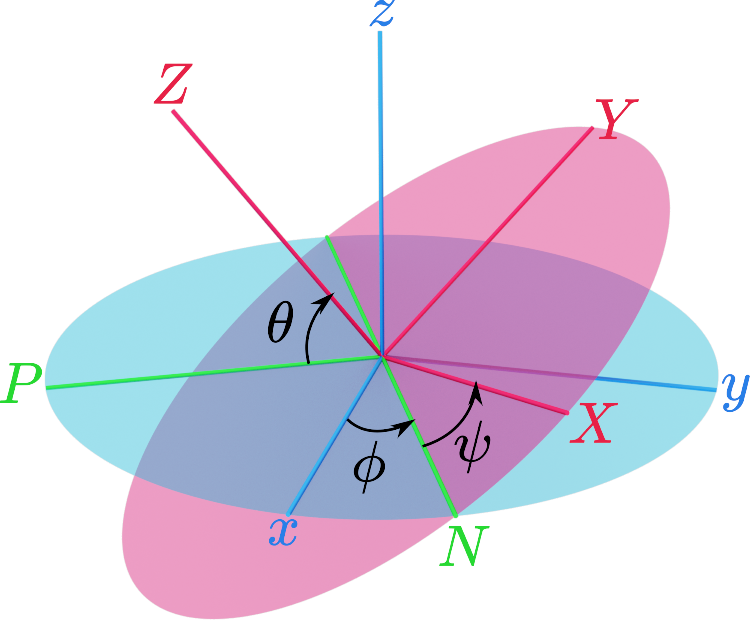
\includegraphics[width=0.5\textwidth]{eulerangles.pdf}
\fi
\end{center}

Although Euler angles are more straightforward to use than quaternions, they are also potentially subject to the ``gimbal lock'' problem:\\
\url{https://en.wikipedia.org/wiki/Gimbal_lock}\\
\noindent{}which arises whenever $\theta \simeq \pm 90^\circ$, including the common case when \emph{the simulated coordinates are near the reference coordinates}.
Therefore, a safe use of Euler angles as collective variables requires the use of restraints to avoid such singularities, such as done in reference~\cite{Fu2017} and in the \href{http://www.ks.uiuc.edu/Training/Tutorials/namd/PLB/tutorial-protein-ligand.pdf}{protein-ligand binding NAMD tutorial}.

The \texttt{eulerPhi} component accepts exactly the same options as \texttt{orientation}, and 
measures the rotation angle from the \textit{x} axis to the \textit{N} axis. This 
angle is expressed in degrees within the periodic range 
$[-180^{\circ}:180^{\circ}]$.

\begin{cvcoptions}
\item %
\dupkey{atoms}{\texttt{eulerPhi}}{colvar|rmsd|atoms}{\texttt{rmsd} 
component}
\item %
\dupkey{refPositions}{\texttt{eulerPhi}}{colvar|rmsd|refPositions}{\texttt{rmsd}
component}
\item %
\dupkey{refPositionsFile}{\texttt{eulerPhi}}{colvar|rmsd|refPositionsFile}{\texttt{rmsd}
component}
\cvnamebasedonly{
\item %

\dupkey{refPositionsCol}{\texttt{eulerPhi}}{colvar|rmsd|refPositionsCol}{\texttt{rmsd}
component}
\item %
	
\dupkey{refPositionsColValue}{\texttt{eulerPhi}}{colvar|rmsd|refPositionsColValue}{\texttt{rmsd}
 component}
}
\end{cvcoptions}


\cvsubsubsec{\texttt{eulerTheta}: Pitch angle from 
references coordinates.}{sec:cvc_eulerTheta}
\labelkey{colvar|eulerTheta}

This component accepts exactly the same options as \texttt{orientation}, and 
measures the rotation angle from the \textit{P} axis to the \textit{Z} axis. 
This angle is expressed in degrees within the range $[-90^{\circ}:90^{\circ}]$.

\textbf{Warning:} When this angle reaches $-90^{\circ}$ or $90^{\circ}$, the 
definition of orientation by euler angles suffers from the gimbal lock issue. 
You may need to apply a restraint to keep \texttt{eulerTheta} away from the 
singularities.

\begin{cvcoptions}
\item %
\dupkey{atoms}{\texttt{eulerTheta}}{colvar|rmsd|atoms}{\texttt{rmsd} 
	component}
\item %
\dupkey{refPositions}{\texttt{eulerTheta}}{colvar|rmsd|refPositions}{\texttt{rmsd}
	component}
\item %
\dupkey{refPositionsFile}{\texttt{eulerTheta}}{colvar|rmsd|refPositionsFile}{\texttt{rmsd}
	component}
\cvnamebasedonly{
\item %

\dupkey{refPositionsCol}{\texttt{eulerTheta}}{colvar|rmsd|refPositionsCol}{\texttt{rmsd}
	component}
\item %

\dupkey{refPositionsColValue}{\texttt{eulerTheta}}{colvar|rmsd|refPositionsColValue}{\texttt{rmsd}
	component}
}
\end{cvcoptions}


\cvsubsubsec{\texttt{eulerPsi}: Yaw angle from 
references coordinates.}{sec:cvc_eulerPsi}
\labelkey{colvar|eulerPsi}

This component accepts exactly the same options as \texttt{orientation}, and 
measures the rotation angle from the \textit{N} axis to the \textit{X} axis. 
This angle is expressed in degrees within the periodic range 
$[-180^{\circ}:180^{\circ}]$.

\begin{cvcoptions}
\item %
\dupkey{atoms}{\texttt{eulerPsi}}{colvar|rmsd|atoms}{\texttt{rmsd} 
	component}
\item %
\dupkey{refPositions}{\texttt{eulerPsi}}{colvar|rmsd|refPositions}{\texttt{rmsd}
	component}
\item %
\dupkey{refPositionsFile}{\texttt{eulerPsi}}{colvar|rmsd|refPositionsFile}{\texttt{rmsd}
	component}
\cvnamebasedonly{
\item %

\dupkey{refPositionsCol}{\texttt{eulerPsi}}{colvar|rmsd|refPositionsCol}{\texttt{rmsd}
	component}
\item %

\dupkey{refPositionsColValue}{\texttt{eulerPsi}}{colvar|rmsd|refPositionsColValue}{\texttt{rmsd}
	component}
}
\end{cvcoptions}


\cvnamebasedonly{

\cvsubsec{Protein structure descriptors}{sec:cvc_protein}

\cvsubsubsec{\texttt{alpha}: $\alpha$-helix content of a protein segment.}{sec:cvc_alpha}
\labelkey{colvar|alpha}

The block \texttt{alpha~\{...\}} defines the
parameters to calculate the helical content of a segment of protein
residues.  The $\alpha$-helical content across the $N+1$ residues
$N_{0}$ to $N_{0}+N$ is calculated by the formula:
\begin{eqnarray}
  \label{eq:colvars_alpha}
  {
    \alpha\left(
      \mathrm{C}_{\alpha}^{(N_{0})},
      \mathrm{O}^{(N_{0})},
      \mathrm{C}_{\alpha}^{(N_{0}+1)},
      \mathrm{O}^{(N_{0}+1)},
      \ldots
      \mathrm{N}^{(N_{0}+5)},
      \mathrm{C}_{\alpha}^{(N_{0}+5)},
      \mathrm{O}^{(N_{0}+5)},
      \ldots
      \mathrm{N}^{(N_{0}+N)},
      \mathrm{C}_{\alpha}^{(N_{0}+N)}
    \right)
  } \; = \; \; \; \; \\ \; \; \; \; {
    \nonumber
    \frac{1}{2(N-2)}
    \sum_{n=N_{0}}^{N_{0}+N-2}
    \mathrm{angf}\left(
        \mathrm{C}_{\alpha}^{(n)},
        \mathrm{C}_{\alpha}^{(n+1)},
        \mathrm{C}_{\alpha}^{(n+2)}\right)
  } \; + \; {
    \frac{1}{2(N-4)}
    \sum_{n=N_{0}}^{N_{0}+N-4}
    \mathrm{hbf}\left(
      \mathrm{O}^{(n)},
      \mathrm{N}^{(n+4)}\right) \mathrm{,}
  } \\
\end{eqnarray}
where the score function for the $\mathrm{C}_{\alpha} -
\mathrm{C}_{\alpha} - \mathrm{C}_{\alpha}$ angle is defined as:
\begin{equation}
  \label{eq:colvars_alpha_Calpha}
  {
    \mathrm{angf}\left(
      \mathrm{C}_{\alpha}^{(n)},
      \mathrm{C}_{\alpha}^{(n+1)},
      \mathrm{C}_{\alpha}^{(n+2)}\right)
  } \; = \; {
    \frac{1 - \left(\theta(
        \mathrm{C}_{\alpha}^{(n)},
        \mathrm{C}_{\alpha}^{(n+1)},
        \mathrm{C}_{\alpha}^{(n+2)}) -
        \theta_{0}\right)^{2} /
      \left(\Delta\theta_{\mathrm{tol}}\right)^{2}}{
      1 - \left(\theta(
        \mathrm{C}_{\alpha}^{(n)},
        \mathrm{C}_{\alpha}^{(n+1)},
        \mathrm{C}_{\alpha}^{(n+2)}) -
        \theta_{0}\right)^{4} /
      \left(\Delta\theta_{\mathrm{tol}}\right)^{4}} \mathrm{,}
  }
\end{equation}
and the score function for the $\mathrm{O}^{(n)} \leftrightarrow
\mathrm{N}^{(n+4)}$ hydrogen bond is defined through a \texttt{hBond}
colvar component on the same atoms.

\begin{cvcoptions}

\item %
  \labelkey{colvar|alpha|residueRange}
  \key
    {residueRange}{%
      \texttt{alpha}}{%
      Potential $\alpha$-helical residues}{%
    ``$<$Initial residue number$>$-$<$Final residue number$>$''}{%
    This option specifies the range of residues on which this
    component should be defined.  The Colvars module looks for the
    atoms within these residues named ``\texttt{CA}'', ``\texttt{N}''
    and ``\texttt{O}'', and raises an error if any of those atoms is
    not found.}

\item %
  \labelkey{colvar|alpha|psfSegID}
  \key
    {psfSegID}{%
    \texttt{alpha}}{%
    PSF segment identifier}{%
    string (max 4 characters)}{%
    This option sets the PSF segment identifier for the residues
    specified in \texttt{residueRange}.  This option is only required
    when PSF topologies are used.}


\item %
  \labelkey{colvar|alpha|hBondCoeff}
  \keydef
    {hBondCoeff}{%
    \texttt{alpha}}{%
    Coefficient for the hydrogen bond term}{%
    positive between 0 and 1}{%
    0.5}{%
    This number specifies the contribution to the total value from the
    hydrogen bond terms.  0 disables the hydrogen bond terms, 1
    disables the angle terms.}

\item %
  \labelkey{colvar|alpha|angleRef}
  \keydef
    {angleRef}{%
    \texttt{alpha}}{%
    Reference $\mathrm{C}_{\alpha} -
    \mathrm{C}_{\alpha} - \mathrm{C}_{\alpha}$ angle}{%
    positive decimal}{%
    88$^{\circ}$}{%
    This option sets the reference angle used in the score function
    (\ref{eq:colvars_alpha_Calpha}).}

\item %
  \labelkey{colvar|alpha|angleTol}
  \keydef
    {angleTol}{%
    \texttt{alpha}}{%
    Tolerance in the $\mathrm{C}_{\alpha} -
    \mathrm{C}_{\alpha} - \mathrm{C}_{\alpha}$ angle}{%
    positive decimal}{%
    15$^{\circ}$}{%
    This option sets the angle tolerance used in the score function
    (\ref{eq:colvars_alpha_Calpha}).}

\item %
  \labelkey{colvar|alpha|hBondCutoff}
  \keydef
    {hBondCutoff}{%
    \texttt{alpha}}{%
    Hydrogen bond cutoff}{%
    positive decimal}{%
    3.3~\AA{}}{%
    Equivalent to the \texttt{cutoff} option in the \texttt{hBond}
    component.}

\item %
  \labelkey{colvar|alpha|hBondExpNumer}
  \keydef
    {hBondExpNumer}{%
    \texttt{alpha}}{%
    Hydrogen bond numerator exponent}{%
    positive integer}{%
    6}{%
    Equivalent to the \texttt{expNumer} option in the \texttt{hBond}
    component.}

\item %
  \labelkey{colvar|alpha|hBondExpDenom}
  \keydef
    {hBondExpDenom}{%
    \texttt{alpha}}{%
    Hydrogen bond denominator exponent}{%
    positive integer}{%
    8}{%
    Equivalent to the \texttt{expDenom} option in the \texttt{hBond}
    component.}

\end{cvcoptions}

This component returns positive values, always comprised between 0
(lowest $\alpha$-helical score) and 1 (highest $\alpha$-helical
score).


\cvsubsubsec{\texttt{dihedralPC}: protein dihedral principal component}{sec:cvc_dihedralPC}
\labelkey{colvar|dihedralPC}

The block \texttt{dihedralPC~\{...\}} defines the
parameters to calculate the projection of backbone dihedral angles within
a protein segment onto a \emph{dihedral principal component}, following
the formalism of dihedral principal component analysis (dPCA) proposed by
Mu et al.\cite{Mu2005} and documented in detail by Altis et
al.\cite{Altis2007}.
Given a peptide or protein segment of $N$ residues, each with Ramachandran
angles $\phi_i$ and $\psi_i$, dPCA rests on a variance/covariance analysis
of the $4(N-1)$ variables $\cos(\psi_1), \sin(\psi_1), \cos(\phi_2), \sin(\phi_2)
\cdots \cos(\phi_N), \sin(\phi_N)$. Note that angles $\phi_1$ and $\psi_N$
have little impact on chain conformation, and are therefore discarded,
following the implementation of dPCA in the analysis software Carma.\cite{Glykos2006}

For a given principal component (eigenvector) of coefficients
$(k_i)_{1 \leq i \leq 4(N-1)}$,
the projection of the current backbone conformation is:
\begin{equation}
\xi = \sum_{n=1}^{N-1} k_{4n-3} \cos(\psi_n) + k_{4n-2} \sin (\psi_n)
+ k_{4n-1} \cos (\phi_{n+1}) + k_{4n} \sin(\phi_{n+1})
\end{equation}

\texttt{dihedralPC} expects the same parameters as the \texttt{alpha}
component for defining the relevant residues (\texttt{residueRange}
and \texttt{psfSegID}) in addition to the following:

\begin{cvcoptions}

\item %
  \dupkey{residueRange}{\texttt{dihedralPC}}{colvar|alpha|residueRange}{\texttt{alpha} component}

\item %
  \dupkey{psfSegID}{\texttt{dihedralPC}}{colvar|alpha|psfSegID}{\texttt{alpha} component}

\item %
  \key
    {vectorFile}{%
    \texttt{dihedralPC}}{%
    File containing dihedral PCA eigenvector(s)}{%
    file name}{%
    A text file containing the coefficients of dihedral PCA eigenvectors on the
    cosine and sine coordinates. The vectors should be arranged in columns,
    as in the files output by Carma.\cite{Glykos2006}}

\item %
  \key
    {vectorNumber}{%
    \texttt{dihedralPC}}{%
    File containing dihedralPCA eigenvector(s)}{%
    positive integer}{%
    Number of the eigenvector to be used for this component.}
\end{cvcoptions}

} % end of \cvnamebasedonly

\cvalchlambdaonly{

\cvsubsec{Alchemical variables for lambda-dynamics}{sec:cvc_alch}

\cvsubsubsec{\texttt{alchLambda}: alchemical lambda parameter.}{sec:cvc_alchlambda}
\labelkey{colvar|alchLambda}

The \texttt{alchLambda~\{\}} block defines a component returning the alchemical lambda parameter
of the back-end simulation in \MDENGINE{}, provided that it is enabled using the appropriate options
of \MDENGINE{}. This coordinate is obtained from the back-end at the beginning of a simulation, and
synchronized from Colvars to \MDENGINE{} at every time step. This enables lambda-dynamics simulations.
The \texttt{alchLambda} block itself takes no parameters, it should be left empty.
In contrast, the \texttt{colvar} block containing it should define the relevant extended-system parameters
to enable lambda dynamics, primarily \refkey{extendedMass}{colvar|extendedMass}:

\begin{cvexampleinput}
\-colvar~\{\\
\-~~name~lambda\\
\-~~extendedLagrangian~on\\
\-~~extendedMass~400\\
\-\\
\-~~alchLambda~\{~\#~Keep~the~line~break\\
\-~~\}\\
\-\}
\end{cvexampleinput}

\cvsubsubsec{\texttt{alchFlambda}: Force on the alchemical lambda parameter.}{sec:cvc_alchFlambda}
\labelkey{colvar|alchFlambda}

The \texttt{alchFlambda~\{\}} block defines a component returning the force exterted on the alchemical
lambda parameter of the back-end simulation in \MDENGINE{}, provided that it is enabled using the appropriate options
of \MDENGINE{}. This coordinate is obtained from the back-end at each time step of a simulation.
The \texttt{alchfLambda} block itself takes no parameters, it should be left empty.
} % end of \cvalchlambdaonly

\cvsubsec{Raw data: building blocks for custom functions}{sec:cvc_raw}

\cvsubsubsec{\texttt{cartesian}: vector of atomic Cartesian coordinates.}{sec:cvc_cartesian}
\labelkey{colvar|cartesian}

The \texttt{cartesian~\{...\}} block defines a component returning a flat vector containing
the Cartesian coordinates of all participating atoms, in the order
$(x_1, y_1, z_1, \cdots, x_n, y_n, z_n)$.

\begin{cvcoptions}
\item %
  \key
    {atoms}{%
    \texttt{cartesian}}{%
    Group of atoms}{%
    \hyperref[sec:colvar_atom_groups]{Atom group}}{%
    Defines the atoms whose coordinates make up the value of the component.
    If \texttt{rotateToReference}, \texttt{centerToReference}, or \texttt{centerToOrigin} are defined, coordinates
    are evaluated within the moving frame of reference.}
\end{cvcoptions}


\cvsubsubsec{\texttt{distancePairs}: set of pairwise distances between two groups.}{sec:cvc_distancePairs}
\labelkey{colvar|distancePairs}

The \texttt{distancePairs~\{...\}} block defines a $N_{\mathrm{1}}\times{}N_{\mathrm{2}}$-dimensional variable that includes all mutual distances between the atoms of two groups.
\ifdefined\cvscriptcallbacks{This can be useful, for example, to develop a new variable defined over two groups, by using the \texttt{scriptedFunction} feature.}\fi

\begin{cvcoptions}
\item %
  \dupkey{group1}{\texttt{distancePairs}}{colvar|distance|group1}{\texttt{distance} component}
\item %
  \simkey{group2}{\texttt{distancePairs}}{group1}
\end{cvcoptions}
This component returns a $N_{\mathrm{1}}\times{}N_{\mathrm{2}}$-dimensional vector of numbers, each ranging from $0$ to the largest possible distance within the chosen boundary conditions.


\cvsubsec{Geometric path collective variables}{sec:cvc_gpath}

The geometric path collective variables define the progress along a path, $s$, and the distance from the path, $z$. These CVs are proposed by Leines and Ensing\cite{Leines2012} , which differ from that\cite{Branduardi2007} proposed by Branduardi et al., and utilize a set of geometric algorithms. The path is defined as a series of frames in the atomic Cartesian coordinate space or the CV space. $s$ and $z$ are computed as

\begin{equation}
s = \frac{m}{M} \pm \frac{1}{2M} \left( \frac{\sqrt{(\mathbf{v}_1 \cdot \mathbf{v}_3)^2-|\mathbf{v}_3|^2 (|\mathbf{v}_1|^2 - |\mathbf{v}_2|^2)}-(\mathbf{v}_1 \cdot \mathbf{v}_3)}{|\mathbf{v}_3|^2} -1 \right)
\end{equation}

\begin{equation}
z = \sqrt{\left(\mathbf{v}_1 + \frac{1}{2}\left(\frac{\sqrt{(\mathbf{v}_1 \cdot \mathbf{v}_3)^2-|\mathbf{v}_3|^2 (|\mathbf{v}_1|^2 - |\mathbf{v}_2|^2)}-(\mathbf{v}_1 \cdot \mathbf{v}_3)}{|\mathbf{v}_3|^2} -1 \right)\mathbf{v}_4 \right)^2}
\end{equation}

where $\mathbf{v}_1 = \mathbf{s}_{m} - \mathbf{z} $ is the vector connecting the current position to the closest frame, $\mathbf{v}_2 = \mathbf{z} - \mathbf{s}_{m-1}$ is the vector connecting the second closest frame to the current position, $\mathbf{v}_3 = \mathbf{s}_{m+1} - \mathbf{s}_{m}$ is the vector connecting the closest frame to the third closest frame, and $\mathbf{v}_4 = \mathbf{s}_m - \mathbf{s}_{m-1}$ is the vector connecting the second closest frame to the closest frame. $m$ and $M$ are the current index of the closest frame and the total number of frames, respectively. If the current position is on the left of the closest reference frame, the $\pm$ in $s$ turns to the positive sign. Otherwise it turns to the negative sign.

The equations above assume: (i) the frames are equidistant and (ii) the second and the third closest frames are neighbouring to the closest frame. When these assumptions are not satisfied, this set of path CV should be used carefully.

\cvsubsubsec{\texttt{gspath}: progress along a path defined in atomic Cartesian coordinate space.}{sec:cvc_gspath}
\labelkey{colvar|gspath}

In the \texttt{gspath~\{...\}} and the \texttt{gzpath~\{...\}} block all vectors, namely $\mathbf{z}$ and $\mathbf{s}_{k}$ are defined in atomic Cartesian coordinate space. More specifically, $\mathbf{z} = \left[\mathbf{r}_{1}, \cdots, \mathbf{r}_{n}\right]$, where $\mathbf{r}_{i}$ is the $i$-th atom specified in the \texttt{atoms} block. $\mathbf{s}_{k} = \left[\mathbf{r}_{k,1}, \cdots, \mathbf{r}_{k,n}\right]$, where $\mathbf{r}_{k,i}$ means the $i$-th atom of the $k$-th reference frame.

\begin{cvcoptions}
\item %
  \key
    {atoms}{%
    \texttt{gspath} and \texttt{gzpath}}{%
    Group of atoms}{%
    \hyperref[sec:colvar_atom_groups]{Atom group}}{%
    Defines the atoms whose coordinates make up the value of the component.}

\item %
  \key
    {refPositionsCol}{%
    \texttt{gspath} and \texttt{gzpath}}{%
    PDB column containing atom flags}{%
    \texttt{O}, \texttt{B}, \texttt{X}, \texttt{Y}, or \texttt{Z}}{%
    If \texttt{refPositionsFileN} is a PDB file that contains all the atoms in the topology, this option may be provided to set which PDB field is used to flag the reference coordinates for \texttt{atoms}.}

\item %
  \key
    {refPositionsFileN}{%
    \texttt{gspath} and \texttt{gzpath}}{%
    File containing the reference positions for fitting}{%
    UNIX filename}{%
		The path is defined by multiple \texttt{refPositionsFile}s which are similiar to \texttt{refPositionsFile} in the \texttt{rmsd} CV. If your path consists of $10$ nodes, you can list the coordinate file (in PDB or XYZ format) from \texttt{refPositionsFile1} to \texttt{refPositionsFile10}.
    }

\item %
  \keydef
    {useSecondClosestFrame}{%
    \texttt{gspath} and \texttt{gzpath}}{%
    Define $\mathbf{s}_{m-1}$ as the second closest frame?}{%
    boolean}{%
    \texttt{on}}{%
    The definition assumes the second closest frame is neighbouring to the closest frame. This is not always true especially when the path is crooked. If this option is set to \texttt{on} (default), $\mathbf{s}_{m-1}$ is defined as the second closest frame. If this option is set to \texttt{off}, $\mathbf{s}_{m-1}$ is defined as the left or right neighbouring frame of the closest frame.
  }

\item %
  \keydef
    {useThirdClosestFrame}{%
    \texttt{gspath} and \texttt{gzpath}}{%
    Define $\mathbf{s}_{m+1}$ as the third closest frame?}{%
    boolean}{%
    \texttt{off}}{%
    The definition assumes the third closest frame is neighbouring to the closest frame. This is not always true especially when the path is crooked. If this option is set to \texttt{on}, $\mathbf{s}_{m+1}$ is defined as the third closest frame. If this option is set to \texttt{off} (default), $\mathbf{s}_{m+1}$ is defined as the left or right neighbouring frame of the closest frame.
  }

\item %
  \key
    {fittingAtoms}{%
    \texttt{gspath} and \texttt{gzpath}}{%
    The atoms that are used for alignment}{%
    Group of atoms}{%
		Before calculating $\mathbf{v}_1$, $\mathbf{v}_2$, $\mathbf{v}_3$ and $\mathbf{v}_4$, the current frame need to be aligned to the corresponding reference frames. This option specifies which atoms are used to do alignment.
    }

\end{cvcoptions}

\cvsubsubsec{\texttt{gzpath}: distance from a path defined in atomic Cartesian coordinate space.}{sec:cvc_gzpath}
\labelkey{colvar|gzpath}

\begin{cvcoptions}

\item %
  \keydef
    {useZsquare}{%
    \texttt{gzpath}}{%
    Compute $z^2$ instead of $z$}{%
    boolean}{%
    \texttt{off}}{%
    $z$ is not differentiable when it is zero. This implementation workarounds it by setting the derivative of $z$ to zero when $z = 0$. Another workaround is set this option to \texttt{on}, which computes $z^2$ instead of $z$, and then $z^2$ is differentiable when it is zero.
  }

\end{cvcoptions}

The usage of \texttt{gzpath} and \texttt{gspath} is illustrated below:

\begin{cvexampleinput}
colvar \{\\
\-~~\# Progress along the path\\
\-~~name gs\\
\-~~\# The path is defined by 5 reference frames (from string-00.pdb to string-04.pdb)\\
\-~~\# Use atomic coordinate from atoms 1, 2 and 3 to compute the path\\
\-~~gspath \{\\
\-~~~~atoms \{atomnumbers \{ 1 2 3 \}\}\\
\-~~~~refPositionsFile1 string-00.pdb\\
\-~~~~refPositionsFile2 string-01.pdb\\
\-~~~~refPositionsFile3 string-02.pdb\\
\-~~~~refPositionsFile4 string-03.pdb\\
\-~~~~refPositionsFile5 string-04.pdb\\
\-~~\}\\
\}\\
\noindent\ttfamily colvar \{\\
\-~~\# Distance from the path\\
\-~~name gz\\
\-~~\# The path is defined by 5 reference frames (from string-00.pdb to string-04.pdb)\\
\-~~\# Use atomic coordinate from atoms 1, 2 and 3 to compute the path\\
\-~~gzpath \{\\
\-~~~~atoms \{atomnumbers \{ 1 2 3 \}\}\\
\-~~~~refPositionsFile1 string-00.pdb\\
\-~~~~refPositionsFile2 string-01.pdb\\
\-~~~~refPositionsFile3 string-02.pdb\\
\-~~~~refPositionsFile4 string-03.pdb\\
\-~~~~refPositionsFile5 string-04.pdb\\
\-~~\}\\
\}
\end{cvexampleinput}


\cvsubsubsec{\texttt{linearCombination}: Helper CV to define a linear combination of other CVs}{sec:cvc_linearCombination}
\labelkey{colvar|linearCombination}

This is a helper CV which can be defined as a linear combination of other CVs. It maybe useful when you want to define the \texttt{gspathCV~\{...\}} and the \texttt{gzpathCV~\{...\}} as combinations of other CVs. Total forces (required by \refkey{ABF}{sec:colvarbias_abf_req}) of this CV are not available.

\cvleptononly{
\cvsubsubsec{\texttt{customColvar}: Helper CV to define a mathematical expression as CV from other CVs}{sec:cvc_customColvar}
\labelkey{colvar|customColvar}}

\cvleptononly{
This is a helper CV which can be defined as a mathematical expression (see \ref{sec:colvar_custom_function}) of other CVs by using \refkey{customFunction}{colvar|customFunction}. Currently only the scalar type of \refkey{customFunction}{colvar|customFunction} is supported. If \refkey{customFunction}{colvar|customFunction} is not provided, this component falls back to \refkey{linearCombination}{colvar|linearCombination}. It maybe useful when you want to define the \texttt{gspathCV~\{...\}}, the \texttt{gzpathCV~\{...\}} and \texttt{NeuralNetwork~\{...\}} as combinations of other CVs. Total forces (required by \refkey{ABF}{sec:colvarbias_abf_req}) of this CV are not available.
}

\cvsubsubsec{\texttt{gspathCV}: progress along a path defined in CV space.}{sec:cvc_gspathCV}
\labelkey{colvar|gspathCV}

In the \texttt{gspathCV~\{...\}} and the \texttt{gzpathCV~\{...\}} block all vectors, namely $\mathbf{z}$ and $\mathbf{s}_{k}$ are defined in CV space.  More specifically, $\mathbf{z} = \left[{\xi}_{1}, \cdots, {\xi}_{n}\right]$, where ${\xi}_{i}$ is the $i$-th CV. $\mathbf{s}_{k} = \left[{\xi}_{k,1}, \cdots, {\xi}_{k,n}\right]$, where ${\xi}_{k,i}$ means the $i$-th CV of the $k$-th reference frame. It should be note that these two CVs requires the \texttt{pathFile} option, which specifies a path file. Each line in the path file contains a set of space-seperated CV value of the reference frame. The sequence of reference frames matches the sequence of the lines.


\begin{cvcoptions}
\item %
  \keydef
    {useSecondClosestFrame}{%
    \texttt{gspathCV} and \texttt{gzpathCV}}{%
    Define $\mathbf{s}_{m-1}$ as the second closest frame?}{%
    boolean}{%
    \texttt{on}}{%
    The definition assumes the second closest frame is neighbouring to the closest frame. This is not always true especially when the path is crooked. If this option is set to \texttt{on} (default), $\mathbf{s}_{m-1}$ is defined as the second closest frame. If this option is set to \texttt{off}, $\mathbf{s}_{m-1}$ is defined as the left or right neighbouring frame of the closest frame.
  }

\item %
  \keydef
    {useThirdClosestFrame}{%
    \texttt{gspathCV} and \texttt{gzpathCV}}{%
    Define $\mathbf{s}_{m+1}$ as the third closest frame?}{%
    boolean}{%
    \texttt{off}}{%
    The definition assumes the third closest frame is neighbouring to the closest frame. This is not always true especially when the path is crooked. If this option is set to \texttt{on}, $\mathbf{s}_{m+1}$ is defined as the third closest frame. If this option is set to \texttt{off} (default), $\mathbf{s}_{m+1}$ is defined as the left or right neighbouring frame of the closest frame.
  }

\item %
  \key
    {pathFile}{%
    \texttt{gspathCV} and \texttt{gzpathCV}}{%
    The file name of the path file.}{%
    UNIX filename}{%
		Defines the nodes or images that constitutes the path in CV space. The CVs of an image are listed in a line of \texttt{pathFile} using space-seperated format. Lines from top to button in \texttt{pathFile} corresponds images from initial to last.
    }

\end{cvcoptions}

\cvsubsubsec{\texttt{gzpathCV}: distance from a path defined in CV space.}{sec:cvc_gzpathCV}
\labelkey{colvar|gzpathCV}

\begin{cvcoptions}

\item %
  \keydef
    {useZsquare}{%
    \texttt{gzpathCV}}{%
    Compute $z^2$ instead of $z$}{%
    boolean}{%
    \texttt{off}}{%
    $z$ is not differentiable when it is zero. This implementation workarounds it by setting the derivative of $z$ to zero when $z = 0$. Another workaround is set this option to \texttt{on}, which computes $z^2$ instead of $z$, and then $z^2$ is differentiable when it is zero.
  }

\end{cvcoptions}

The usage of \texttt{gzpathCV} and \texttt{gspathCV} is illustrated below:

\begin{cvexampleinput}
\-colvar \{\\
\-~~\# Progress along the path\\
\-~~name gs\\
\-~~\# Path defined by the CV space of two dihedral angles\\
\-~~gspathCV \{\\
\-~~~~pathFile ./path.txt\\
\-~~~~dihedral \{\\
\-~~~~~~name 001\\
\-~~~~~~group1 \{atomNumbers \{5\}\}\\
\-~~~~~~group2 \{atomNumbers \{7\}\}\\
\-~~~~~~group3 \{atomNumbers \{9\}\}\\
\-~~~~~~group4 \{atomNumbers \{15\}\}\\
\-~~~~\}\\
\-~~~~dihedral \{\\
\-~~~~~~name 002\\
\-~~~~~~group1 \{atomNumbers \{7\}\}\\
\-~~~~~~group2 \{atomNumbers \{9\}\}\\
\-~~~~~~group3 \{atomNumbers \{15\}\}\\
\-~~~~~~group4 \{atomNumbers \{17\}\}\\
\-~~~~\}\\
\-~~\}\\
\}\\
\\
\-colvar \{\\
\-~~\# Distance from the path\\
\-~~name gz\\
\-~~gzpathCV \{\\
\-~~~~pathFile ./path.txt\\
\-~~~~dihedral \{\\
\-~~~~~~name 001\\
\-~~~~~~group1 \{atomNumbers \{5\}\}\\
\-~~~~~~group2 \{atomNumbers \{7\}\}\\
\-~~~~~~group3 \{atomNumbers \{9\}\}\\
\-~~~~~~group4 \{atomNumbers \{15\}\}\\
\-~~~~\}\\
\-~~~~dihedral \{\\
\-~~~~~~name 002\\
\-~~~~~~group1 \{atomNumbers \{7\}\}\\
\-~~~~~~group2 \{atomNumbers \{9\}\}\\
\-~~~~~~group3 \{atomNumbers \{15\}\}\\
\-~~~~~~group4 \{atomNumbers \{17\}\}\\
\-~~~~\}\\
\-~~\}\\
\}
\end{cvexampleinput}


\cvsubsec{Arithmetic path collective variables}{sec:cvc_apathCV}

The arithmetic path collective variable in CV space uses a similar formula as 
the one proposed by Branduardi\cite{Branduardi2007} et al., except that it 
computes $s$ and $z$ in CV space instead of RMSDs in Cartesian space. Moreover, 
this implementation allows different coefficients for each CV components as 
described in \cite{Hovan2019}. Assuming a path is composed of $N$ reference 
frames and defined in an $M$-dimensional CV space, then the equations of $s$ 
and $z$ of the path are

\begin{equation}
s = \frac{1}{N-1}\frac{\sum_{i=0}^{N-1} i \exp\left(-\lambda\sum_{j=1}^{M} 
c_j^2 \left(x_j-x_{i,j}\right)^2\right)}{\sum_{i=0}^{N-1} 
\exp\left(-\lambda\sum_{j=1}^{M} c_j^2 \left(x_j-x_{i,j}\right)^2\right)}
\label{eq:apath_s}
\end{equation}

\begin{equation}
z = -\frac{1}{\lambda} \ln \left(\sum_{i=0}^{N-1} 
\exp\left(-\lambda\sum_{j=1}^{M} c_j^2 \left(x_j-x_{i,j}\right)^2 \right)\right)
\label{eq:apath_z}
\end{equation}
where $c_j$ is the coefficient(weight) of the $j$-th CV, $x_{i,j}$ is the value 
of $j$-th CV of $i$-th reference frame and $x_{j}$ is the value of $j$-th CV of 
current frame. $\lambda$ is a parameter to smooth the variation of $s$ and $z$. 
It should be noted that the index $i$ ranges from $0$ to $N-1$, and the 
definition of $s$ is normalized by $1/(N-1)$. Consequently, the scope of $s$ is 
$[0:1]$.

\cvsubsubsec{\texttt{aspathCV}: progress along a path defined in CV space.}{sec:cvc_aspathCV}

This colvar component computes the $s$ variable.

\labelkey{colvar|aspathCV}

\begin{cvcoptions}
\item %
  \keydef
    {weights}{%
    \texttt{aspathCV} and \texttt{azpathCV}}{%
    Coefficients of the collective variables}{%
    space-separated numbers in a \texttt{\{...\}} block}{%
    \texttt{\{1.0 ...\}}}{%
    Define the coefficients. The $j$-th value in the \texttt{\{...\}} block corresponds the $c_{j}$ in the equations.
  }

\item %
  \keydef
    {lambda}{%
    \texttt{aspathCV} and \texttt{azpathCV}}{%
    Smoothness of the variation of $s$ and $z$}{%
    decimal}{%
    inverse of the mean square displacements of successive reference frames}{%
    The value of $\lambda$ in the equations.
  }

\item %
  \key
    {pathFile}{%
    \texttt{aspathCV} and \texttt{azpathCV}}{%
    The file name of the path file.}{%
    UNIX filename}{%
		Defines the nodes or images that constitutes the path in CV space. The CVs of an image are listed in a line of \texttt{pathFile} using space-separated format. Lines from top to button in \texttt{pathFile} corresponds images from initial to last.
    }

\end{cvcoptions}

\cvsubsubsec{\texttt{azpathCV}: distance from a path defined in CV space.}{sec:cvc_azpathCV}

This colvar component computes the $z$ variable. Options are the same as in \ref{sec:cvc_aspathCV}.

The usage of \texttt{azpathCV} and \texttt{aspathCV} is illustrated below:

\begin{cvexampleinput}
colvar \{\\
\-~~\# Progress along the path\\
\-~~name as\\
\-~~\# Path defined by the CV space of two dihedral angles\\
\-~~aspathCV \{\\
\-~~~~pathFile ./path.txt\\
\-~~~~weights \{1.0 1.0\}\\
\-~~~~lambda 0.005\\
\-~~~~dihedral \{\\
\-~~~~~~name 001\\
\-~~~~~~group1 \{atomNumbers \{5\}\}\\
\-~~~~~~group2 \{atomNumbers \{7\}\}\\
\-~~~~~~group3 \{atomNumbers \{9\}\}\\
\-~~~~~~group4 \{atomNumbers \{15\}\}\\
\-~~~~\}\\
\-~~~~dihedral \{\\
\-~~~~~~name 002\\
\-~~~~~~group1 \{atomNumbers \{7\}\}\\
\-~~~~~~group2 \{atomNumbers \{9\}\}\\
\-~~~~~~group3 \{atomNumbers \{15\}\}\\
\-~~~~~~group4 \{atomNumbers \{17\}\}\\
\-~~~~\}\\
\-~~\}\\
\}\\
\\
colvar \{\\
\-~~\# Distance from the path\\
\-~~name az\\
\-~~azpathCV \{\\
\-~~~~pathFile ./path.txt\\
\-~~~~weights \{1.0 1.0\}\\
\-~~~~lambda 0.005\\
\-~~~~dihedral \{\\
\-~~~~~~name 001\\
\-~~~~~~group1 \{atomNumbers \{5\}\}\\
\-~~~~~~group2 \{atomNumbers \{7\}\}\\
\-~~~~~~group3 \{atomNumbers \{9\}\}\\
\-~~~~~~group4 \{atomNumbers \{15\}\}\\
\-~~~~\}\\
\-~~~~dihedral \{\\
\-~~~~~~name 002\\
\-~~~~~~group1 \{atomNumbers \{7\}\}\\
\-~~~~~~group2 \{atomNumbers \{9\}\}\\
\-~~~~~~group3 \{atomNumbers \{15\}\}\\
\-~~~~~~group4 \{atomNumbers \{17\}\}\\
\-~~~~\}\\
\-~~\}\\
\}
\end{cvexampleinput}


\ifdefined\cvvmdornamd{
\cvsubsubsec{Path collective variables in Cartesian coordinates}{sec:apath_scripted}

The path collective variables defined by Branduardi et al.~\cite{Branduardi2007}
are based on RMSDs in Cartesian coordinates.
Noting $d_i$ the RMSD between the current set of Cartesian coordinates and those of image number $i$ of the path:

\begin{equation}
s = \frac{1}{N-1} \frac{\sum_{i=1}^{N} (i-1) \exp\left(-\lambda d_i^2\right)}
{\sum_{i=1}^{N} \exp\left(-\lambda d_i^2\right)}
\end{equation}

\begin{equation}
z = -\frac{1}{\lambda} \ln \left(\sum_{i=1}^{N} \exp(-\lambda d_i^2)\right)
\end{equation}

where $\lambda$ is the smoothing parameter.


These coordinates are implemented as Tcl-scripted combinations of \texttt{rmsd} components.
The implementation is available as file \texttt{colvartools/pathCV.tcl}, and
an example is provided in file \texttt{examples/10\_pathCV.namd} of the Colvars public repository.
It implements an optimization procedure, whereby the distance to a given image is only calculated if its contribution
to the sum is larger than a user-defined \texttt{tolerance} parameter.
All distances are calculated every \texttt{freq} timesteps to update the list of nearby images.
}\fi

\cvsubsubsec{\texttt{aspath}: progress along a path defined in atomic Cartesian coordinate space.}{sec:cvc_aspath}
\labelkey{colvar|aspath}

This CV computes a special case of Eq. \ref{eq:apath_s}, where $x_j$ is the
$j$-th atomic position, $x_{i,j}$ is the $j$-th atomic position of the $i$-th
reference frame. The subtraction $x_j - x_{i,j}$ is actually calculated as
$\mathbf{x}_j - R_i\mathbf{x}_{i,j}$, where $\mathrm{R}_i$ is a 3x3 rotation
matrix that minimizes the RMSD between the current atomic positions of
simulation and the $i$-th reference frame. Bold $\mathbf{x}_j$ is used since
an atomic position is a vector.

\ifdefined\cvvmdornamd{
For NAMD and VMD users, this component can be regarded as an improved C++
implementation of the PCV progress component of the Tcl-scripted version
(see \ref{sec:apath_scripted}).
}\fi

\begin{cvcoptions}
\item %
  \key
    {atoms}{%
    \texttt{aspath} and \texttt{azpath}}{%
    Group of atoms}{%
    \hyperref[sec:colvar_atom_groups]{Atom group}}{%
    Defines the atoms whose coordinates make up the value of the component.}

\item %
  \key
    {refPositionsCol}{%
    \texttt{aspath} and \texttt{azpath}}{%
    PDB column containing atom flags}{%
    \texttt{O}, \texttt{B}, \texttt{X}, \texttt{Y}, or \texttt{Z}}{%
    If \texttt{refPositionsFileN} is a PDB file that contains all the atoms in the topology, this option may be provided to set which PDB field is used to flag the reference coordinates for \texttt{atoms}.}

\item %
  \key
    {refPositionsFileN}{%
    \texttt{aspath} and \texttt{azpath}}{%
    File containing the reference positions for fitting}{%
    UNIX filename}{%
		The path is defined by multiple \texttt{refPositionsFile}s which are similiar to \texttt{refPositionsFile} in the \texttt{rmsd} CV. If your path consists of $10$ nodes, you can list the coordinate file (in PDB or XYZ format) from \texttt{refPositionsFile1} to \texttt{refPositionsFile10}.
    }

\item %
  \key
    {fittingAtoms}{%
    \texttt{aspath} and \texttt{azpath}}{%
    The atoms that are used for alignment}{%
    Group of atoms}{%
		Before calculating $\mathbf{v}_1$, $\mathbf{v}_2$, $\mathbf{v}_3$ and $\mathbf{v}_4$, the current frame need to be aligned to the corresponding reference frames. This option specifies which atoms are used to do alignment.
    }

\end{cvcoptions}

\cvsubsubsec{\texttt{azpath}: distance from a path defined in atomic Cartesian coordinate space.}{sec:cvc_azpath}
\labelkey{colvar|azpath}

Similar to \refkey{aspath}{colvar|aspath}, this CV computes a special case of Eq.
\ref{eq:apath_z}, and shares the same options as \refkey{aspath}{colvar|aspath}.

The usage of \texttt{azpath} and \texttt{aspath} is illustrated below:

\begin{cvexampleinput}
colvar \{\\
\-~~\# Progress along the path\\
\-~~name as\\
\-~~\# The path is defined by 5 reference frames (from string-00.pdb to string-04.pdb)\\
\-~~\# Use atomic coordinate from atoms 1, 2 and 3 to compute the path\\
\-~~aspath \{\\
\-~~~~atoms \{atomnumbers \{ 1 2 3 \}\}\\
\-~~~~refPositionsFile1 string-00.pdb\\
\-~~~~refPositionsFile2 string-01.pdb\\
\-~~~~refPositionsFile3 string-02.pdb\\
\-~~~~refPositionsFile4 string-03.pdb\\
\-~~~~refPositionsFile5 string-04.pdb\\
\-~~\}\\
\}\\
\noindent\ttfamily colvar \{\\
\-~~\# Distance from the path\\
\-~~name az\\
\-~~\# The path is defined by 5 reference frames (from string-00.pdb to string-04.pdb)\\
\-~~\# Use atomic coordinate from atoms 1, 2 and 3 to compute the path\\
\-~~azpath \{\\
\-~~~~atoms \{atomnumbers \{ 1 2 3 \}\}\\
\-~~~~refPositionsFile1 string-00.pdb\\
\-~~~~refPositionsFile2 string-01.pdb\\
\-~~~~refPositionsFile3 string-02.pdb\\
\-~~~~refPositionsFile4 string-03.pdb\\
\-~~~~refPositionsFile5 string-04.pdb\\
\-~~\}\\
\}
\end{cvexampleinput}

\cvsubsec{Dense neural network in CV space (MLCV)}{sec:cvc_neuralNetwork}
\labelkey{colvar|NeuralNetwork}

This colvar component computes a non-linear combination of other scalar colvar components, where the transformation is defined by a dense neural network.\cite{Chen2022}
The network can be optimized using any framework, and its parameters are provided to Colvars in plain text files, as detailed below.
An example Python script to export the parameters of a TensorFlow model is provided in \texttt{colvartools/extract\_weights\_biases.py} in the Colvars source tree.

\begin{figure}[!ht]
	\centering
	\ifdefined\HCode{\HCode{<img class="neural_network" src="dense_nn.png" alt="Dense neural network">}}\else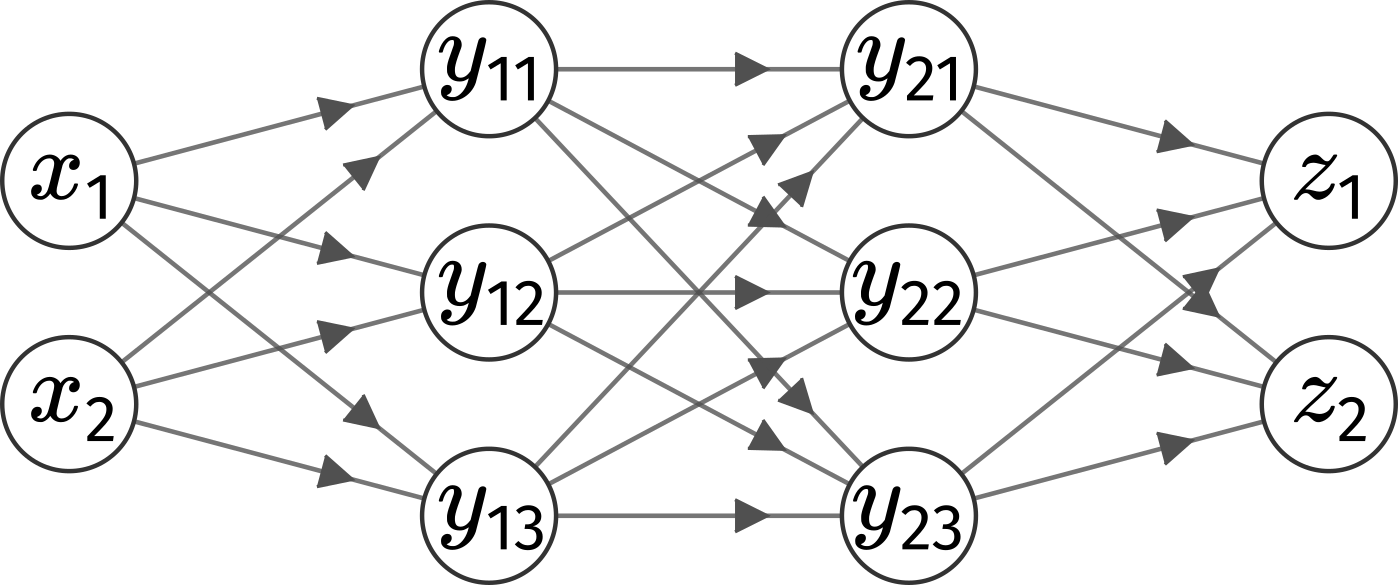
\includegraphics[width=9cm]{dense_nn}\fi
	\caption[Graphical representation of an example dense neural network.]{Graphical representation of an example dense neural network with two hidden layers $y_1$ and $y_2$. Both the input layer $x$ and the output layer $z$ have two nodes. The input nodes can be any existing scalar CVs.
	}
	\label{fig:dense_nn}
\end{figure}

The output of the $j$-th node of a $k$-th layer that has $N_k$ nodes is computed by

\begin{equation}
y_{k,j}=f_{k}\left(\sum_{i=1}^{N_{k-1}} w_{(k,j),(k-1,i)} y_{k-1,i} + b_{k,j}\right),
\end{equation}

where $f_{k}$ is the activation function of the $k$-th layer, $w_{(k,j),(k-1,i)}$ is the weight of $j$-th node with respect to the $i$-th output of previous layer, and $b_{k,j}$ is the bias of $j$-th node of $k$-th layer.


\begin{cvcoptions}

\item %
  \labelkey{colvar|NeuralNetwork|output_component}
  \key
  {output\_component}%
  {\texttt{NeuralNetwork}}%
  {The $j$-th node of the output or the last layer}%
  {integer starting from 0}%
  {The value of this option specifies the output node to be used as
   the value of this CV.}

\item %
  \labelkey{colvar|NeuralNetwork|layeri_WeightsFile}
  \key
  {layer$i$\_WeightsFile}%
  {\texttt{NeuralNetwork}}%
  {The weights from layer $i-1$ to layer $i$}%
  {UNIX filename}%
  {The letter $i$ in this option needs to be replaced with the indexing
   number starting from 1, for example, \texttt{layer1\_WeightsFile} and
   \texttt{layer2\_WeightsFile}. The value of this option specifies a
   plain text file containing the weights from layer $i-1$ to layer $i$.
   In the file, the number at $k$-th column and $l$-th row represents the
   weight from node $k$ at layer $i-1$ to node $l$ at layer $i$.}

\item %
  \labelkey{colvar|NeuralNetwork|layeri_BiasesFile}
  \key
  {layer$i$\_BiasesFile}%
  {\texttt{NeuralNetwork}}%
  {The biases from layer $i-1$ to layer $i$}%
  {UNIX filename}%
  {The letter $i$ in this option needs to be replaced with the indexing
   number starting from 1, for example, \texttt{layer1\_BiasesFile} and
   \texttt{layer2\_BiasesFile}. The value of this option specifies a plain
   text file containing the weights of layer $i$. The file should have
   only one column, where the number at $l$-th row represents the bias of
   node $l$ from layer $i-1$ to layer $i$.}

\item %
  \labelkey{colvar|NeuralNetwork|layeri_activation}
  \key
  {layer$i$\_activation}%
  {\texttt{NeuralNetwork}}%
  {The activation function from layer $i-1$ to layer $i$}%
  {\texttt{tanh}, \texttt{sigmoid}, \texttt{linear}, \texttt{relu}, \texttt{lrelu100}, \texttt{elu} }%
  {The letter $i$ in this option needs to be replaced with the indexing
   number starting from 1, for example, \texttt{layer1\_activation} and
   \texttt{layer2\_activation}. The activation function from layer $i-1$
   to layer $i$. Available choices are \texttt{tanh},
  \texttt{sigmoid}, \texttt{linear} (identity), \texttt{relu}, \texttt{lrelu100}
  (a leaky rely with coefficients $10^{-2}$ and 1), and \texttt{elu} (with coefficient 1).}

\item %
  \labelkey{colvar|NeuralNetwork|layeri_custom_activation}
  \key
  {layer$i$\_custom\_activation}%
  {\texttt{NeuralNetwork}}%
  {An alternative custom expression as the activation function
   from layer $i-1$ to layer $i$}%
  {string}%
  {Mathematical expression to define the activation function from layer $i-1$
   to layer $i$. The input value must be written as \texttt{x}. For example,
   the ELU activation function can be expressed as
   \texttt{select(step(x), alpha*(exp(x)-1), x)}.
   For details of the expression syntax, see \refkey{customFunction}{colvar|customFunction}.
   This option is mutually exclusive with
   \refkey{colvar|NeuralNetwork|layeri\_activation}.}

\end{cvcoptions}

An example of configuration using \texttt{NeuralNetwork} is shown below:

\bigskip
{%
% verbatim can't appear within commands
\noindent\ttfamily colvar \{\\
\-~~\# Define a neural network with 2 layers\\
\-~~\# The inputs are two torsion angles\\
\-~~\# and the first node at the output layer is used as the final CV\\
\-~~name nn\_output\_1\\
\-~~NeuralNetwork \{\\
\-~~~~output\_component 0\\
\-~~~~layer1\_WeightsFile      dense\_1\_weights.txt\\
\-~~~~layer1\_BiasesFile       dense\_1\_biases.txt\\
\-~~~~layer1\_activation       tanh\\
\-~~~~layer2\_WeightsFile      dense\_2\_weights.txt\\
\-~~~~layer2\_BiasesFile       dense\_2\_biases.txt\\
\-~~~~layer2\_activation       tanh\\
\-~~~~\# The component coefficient is used for normalization\\
\-~~~~componentCoeff 180.0\\
\-~~~~dihedral \{\\
\-~~~~~~name 001\\
\-~~~~~~\# normalization factor 1.0/180.0\\
\-~~~~~~componentCoeff 0.00555555555555555556\\
\-~~~~~~group1 \{atomNumbers \{5\}\}\\
\-~~~~~~group2 \{atomNumbers \{7\}\}\\
\-~~~~~~group3 \{atomNumbers \{9\}\}\\
\-~~~~~~group4 \{atomNumbers \{15\}\}\\
\-~~~~\}\\
\-~~~~dihedral \{\\
\-~~~~~~name 002\\
\-~~~~~~\# normalization factor 1.0/180.0\\
\-~~~~~~componentCoeff 0.00555555555555555556\\
\-~~~~~~group1 \{atomNumbers \{7\}\}\\
\-~~~~~~group2 \{atomNumbers \{9\}\}\\
\-~~~~~~group3 \{atomNumbers \{15\}\}\\
\-~~~~~~group4 \{atomNumbers \{17\}\}\\
\-~~~~\}\\
\-~~\}\\
\}}


\ifdefined\cvvmdornamd{

\cvsubsec{Volumetric map-based variables}{sec:cvc_volmaps}

Volumetric maps of the Cartesian coordinates, typically defined as mesh grid along the three Cartesian axes, may be used to define collective variables.
\cvnamdonly{In NAMD this feature implemented as an interface between Colvars and \href{https://www.ks.uiuc.edu/Research/namd/2.14/ug/node43.html}{GridForces}.}
Please cite \cite{Fiorin2020} when using this implementation of collective variables based on volumetric maps.

\cvsubsubsec{\texttt{mapTotal}: total value of a volumetric map}{sec:cvc_map_total}
\labelkey{colvar|mapTotal}

Given a function of the Cartesian coordinates $\phi(\mathbf{x}) = \phi(x, y, z)$, a \texttt{mapTotal} collective variable component $\Phi(\mathbf{X})$ is defined as the sum of the values of the function $\phi(\mathbf{x})$ evaluated at the coordinates of each atom, $\mathbf{x}_{i}$:
\begin{equation}
  \label{eq:cvc_map_total}
  \Phi\left(\mathbf{X}\right) = \sum_{i=1}^{N} w_i \phi\left(\mathbf{x}_{i}\right)
\end{equation}
\noindent{}where $w_i$ are weights assigned to each variable (1 by default).
This formulation allows, for example, to ``count'' the number of atoms within a region of space by using a positive-valued function $\phi\left(\mathbf{x}\right)$, such as for example the number of water molecules in a hydrophobic cavity \cite{Fiorin2020}.\\

Because the volumetric map itself and the atoms affected by it are defined externally to Colvars, this component has a very limited number of keywords.

\begin{cvcoptions}
\cvnamdonly{
\item %
  \labelkey{colvar|mapTotal|mapName}
  \key
    {mapName}{%
    \texttt{mapTotal}}{%
    Specify the name of the volumetric map to use as a colvar}{%
    string}{%
    The value of this option specifies the label of the volumetric map to use for this collective variable component.
    This label must identify a map already loaded in NAMD via \texttt{mGridForcePotFile}, and the corresponding value of \texttt{mGridForceScale} must be set to (0, 0, 0), so that its collective force is computed dynamically.
  }
}

\item %
  \labelkey{colvar|mapTotal|mapID}
  \key
    {mapID}{%
    \texttt{mapTotal}}{%
    Specify the numeric index of the volumetric map to use as a colvar}{%
    non-negative integer}{%
    The value of this option specifies the numeric index of the volumetric map to use for this collective variable component.
    The map referred to must be already loaded before using this option.
    \cvnamdonly{This option is mutually exclusive with \refkey{mapName}{colvar|mapTotal|mapName}; if the latter is given, the numeric ID is obtained internally from \MDENGINE{}.}
  }

\item %
  \labelkey{colvar|mapTotal|atoms}
  \key
    {atoms}{%
    \texttt{mapTotal}}{%
    Group of atoms defining this function}{%
    \hyperref[sec:colvar_atom_groups]{Atom group}}{%
    If defined, this option allows defining the set of atoms to be aligned onto the volumetric map following the syntax described in section \ref{sec:colvar_atom_groups}.
    This also allows, for instance, to express the volumetric map in a rotated frame of reference (see \ref{sec:colvar_atom_groups_ref_frame}).
    \cvvmdonly{In VMD, this definition is required, otherwise the \texttt{mapTotal} value is identically zero.}
    \cvnamdonly{In NAMD, this keyword is optional; unless a frame of reference other than the laboratory is needed, it is computationally much more efficient to select atoms via \href{https://www.ks.uiuc.edu/Research/namd/2.14/ug/node43.html}{GridForces} keywords.}
    }

\item %
  \labelkey{colvar|mapTotal|atomWeights}
  \keydef
    {atoms}{%
    \texttt{mapTotal}}{%
    Weights to assign to each atom}{%
    list of space-separated decimals}{%
    all weights equal to 1}{%
    If defined, the value of this option assigns weights $w_i$ to the individual atoms in a \texttt{mapTotal} variable.
    This option requires defining \texttt{atoms} explicitly, and the number of weights must match the number of atoms.
    }

\end{cvcoptions}

\cvnamdonly{
\noindent\textbf{Example: biasing the number of molecules inside a cavity using a volumetric map.}

Firstly, a volumetric map that has a value of 1 inside the cavity and 0 outside should be prepared.
A reasonable starting point may be obtained, for example, with VMD: using an existing trajectory where the cavity is occupied by solvent and a spatial selection that identifies all the molecules within the cavity, \texttt{volmap occupancy -allframes -combine max} computes the occupancy map as a step function (values 1 or 0), and \texttt{volutil -smooth \ldots} makes it a continuous map, suitable for use as a MD simulation bias.
A PDB file defining the selection (for example, where all water oxygens and ions have an occupancy of 1 and other atoms 0) is also prepared using VMD.
Both the map file and the atom selection file are then loaded via the \texttt{mGridForcePotFile} and related NAMD commands:

\begin{mdexampleinput}
  \-mGridForce yes\\
  \-mGridForcePotFile Cavity cavity.dx~~~\# OpenDX map file\\
  \-mGridForceFile Cavity water-sel.pdb~~\# PDB file used for atom selection\\
  \-mGridForceCol Cavity O~~~~~~~~~~~~~~~\# Use the occupancy column of the PDB file\\
  \-mGridForceChargeCol Cavity B~~~~~~~~~\# Use beta as ``charge'' (default: electric charge)\\
  \-mGridForceScale Cavity 0.0 0.0 0.0~~~\# Do not use GridForces for this map\\
\end{mdexampleinput}

The value of \texttt{mGridForceScale} is particularly important, because it determines the GridForces force constant for the ``Cavity'' map.
A non-zero value enables a conventional GridForces calculation, where the force constant remains fixed within each \texttt{run} command and the forces on the atoms depend only on their positions in space.
However, setting \texttt{mGridForceScale} to zero signals to NAMD that the force acting through the volumetric map may be computed dynamically, as part of a collective-variable biasing scheme.
To do so, the map labeled ``Cavity'' needs to be referred to in the Colvars configuration:\\

\begin{mdexampleinput}
  \-cv config "\\
  \-colvar \{\\
  \-\-~~name n\_waters\\
  \-\-~~mapTotal \{\\
  \-\-~~~~mapName Cavity  \# Same label as the GridForce map\\
  \-\-~~\}\\
  \-\}"
\end{mdexampleinput}


The variable ``\texttt{n\_waters}'' may then be used with any of the enhanced sampling methods available (\ref{sec:colvarbias}): new forces applied to it at each simulation step will be transmitted to the corresponding atoms within the same step.
} % \cvnamdonly{}


\cvsubsubsec{Multiple volumetric maps collective variables}{sec:cvc_multimap}

To study processes that involve changes in shape of a macromolecular aggregate (for example, deformations of lipid membranes) it is useful to define collective variables based on more than one volumetric map at a time, measuring the relative similarity with each map while still achieving correct thermodynamic sampling of each state.

This is achieved by combining multiple \texttt{mapTotal} components, each based on a differently-shaped volumetric map, into a single collective variable $\xi$.
To track transitions between states, the contribution of each map to $\xi$ should be discriminated from the others, for example by assigning to it a different weight.
The ``Multi-Map'' progress variable \cite{Fiorin2020} uses a weight sum of these components, using linearly-increasing weights:
\begin{equation}
  \label{eq:cvc_multi_map}
    \xi\left(\mathbf{X}\right) = \sum_{k=1}^{K} k \Phi_{k}\left(\mathbf{X}\right) = \sum_{k=1}^{K} k \sum_{i=1}^{N}\phi_{k}\left(\mathbf{x}_{i}\right)
\end{equation}
\noindent{}where $K$ is the number of maps employed and each $\Phi_k$ is a \texttt{mapTotal} component.

Here is a link to the \textbf{Multi-Map tutorial} page: \url{https://colvars.github.io/multi-map/multi-map.html}\\
An example configuration for illustration purposes is also included below.

\noindent\textbf{Example: transitions between macromolecular shapes using volumetric maps.}\\
A series of map files, each representing a different shape, is loaded into NAMD:\\
\begin{mdexampleinput}
  \-mGridForce yes\\
  \-for \{ set k 1 \} \{ \$k <= \$K \} \{ incr k \} \{\\
  \-~~mGridForcePotFile Shape\_\$k map\_\$k.dx~~~\# Density map of the k-th state\\
  \-~~mGridForceFile Shape\_\$k atoms.pdb~~~\# PDB file used for atom selection\\
  \-~~mGridForceCol Shape\_\$k O~~~\# Use the occupancy column of the PDB file atoms.pdb\\
  \-~~mGridForceChargeCol Shape\_\$k B~~~\# Use beta as ``charge'' (default: electric charge)\\
  \-~~mGridForceScale Shape\_\$k 0.0 0.0 0.0~~\# Do not use GridForces for this map\\
  \-\}
\end{mdexampleinput}

The GridForces maps thus loaded are then used to define the Multi-Map collective variable, with coefficients $\xi_k = k$ \cite{Fiorin2020}:\\
\begin{mdexampleinput}
  \-\# Collect the definition of all components into one string\\
  \-set components "\\
  \-for \{ set k 1 \} \{ \$k <= \$K \} \{ incr k \} \{\\
  \-~~set components "\$\{components\}\\
  \-~~mapTotal \{\\
  \-~~~~mapName Shape\_\$k\\
  \-~~~~componentCoeff \$k\\
  \-~~\}\\
  \-\}\\
  \-"\\
  \-\# Use this string to define the variable\\
  \-cv config "\\
  \-colvar \{\\
  \-\-~~name shapes\\
  \-\-~~\$\{components\}\\
  \-\}"
\end{mdexampleinput}

The above example illustrates a use case where a weighted sum (i.e.{} a linear combination) is used to define a single variable from multiple components.
Depending on the problem under study, non-linear functions may be more appropriate.
These may be defined a custom functions if implemented\cvleptononly{ (see \ref{sec:colvar_custom_function})}\cvscriptonly{, or scripted functions (see \ref{sec:colvar_scripted})}.

}\fi % \ifdefined\cvvmdornamd{}


\cvsubsec{Shared keywords for all components}{sec:cvc_common}

The following options can be used for any of the above colvar components in order to obtain a polynomial combination\ifdefined\cvscriptcallbacks{ or any user-supplied function provided by \refkey{scriptedFunction}{sec:cvc_superp}}\fi.
\begin{itemize}
\item %
  \keydef
    {name}{%
    any component}{%
    Name of this component}{%
    string}{%
    type of component + numeric id}{%
    The name is an unique case-sensitive string which allows the
    Colvars module to identify this component. 
    \ifdefined\cvscriptcallbacks{This is useful, for example, when combining multiple components via a \texttt{scriptedFunction}.}\fi
    \cvleptononly{It also defines the variable name representing the component's value in a \refkey{customFunction}{colvar|customFunction} expression.}}

\item %
  \keydef
    {scalable}{%
    any component}{%
    Attempt to calculate this component in parallel?}{%
    boolean}{%
    \texttt{on}, if available}{%
    If set to \texttt{on} (default), the Colvars module will attempt to calculate this component in parallel to reduce overhead.
    Whether this option is available depends on the type of component: currently supported are \texttt{distance}, \texttt{distanceZ}, \texttt{distanceXY}, \texttt{distanceVec}, \texttt{distanceDir}, \texttt{angle} and \texttt{dihedral}.
    This flag influences computational cost, but does not affect numerical results: therefore, it should only be turned off for debugging or testing purposes.
  }
\end{itemize}


\cvsubsec{Periodic components}{sec:cvc_periodic}

Certain components, such as \refkey{dihedral}{colvar|dihedral} or
\refkey{dihedral}{colvar|spinAngle}, compute angles that lie in a periodic interval between
$-180^\circ$ and $180^\circ$.  When computing pairwise distances between values of those angles
(e.g.\ for the sake of computing restraint potentials, or sampling PMFs), periodicity is taken into
account by following the minimum-image convention.

Additionally, several other components, such as \refkey{distanceZ}{colvar|distanceZ}, support
optional periodicity if this is provided in the configuration.

The following keywords can be used within periodic components\cvleptononly{, or within custom
  variables (\ref{sec:colvar_custom_function})}\cvscriptonly{, or wthin scripted variables
  \ref{sec:colvar_scripted}}).

\begin{itemize}
\item %
  \labelkey{colvar|cvc|period}
  \keydef
    {period}{%
    components with optional periodicity}{%
    Period of the component}{%
    positive decimal}{%
    0.0, unless otherwise stated}{%
    Setting this number enables the treatment of as
    a periodic component: by default, \texttt{distanceZ} is not
    considered periodic.  The keyword is supported, but irrelevant
    within \texttt{dihedral} or \texttt{spinAngle}, because their
    period is always 360~degrees.}

\item %
  \labelkey{colvar|cvc|wrapAround}
  \keydef
    {wrapAround}{%
    periodic components}{%
    Center of the wrapping interval for periodic variables}{%
    decimal}{%
    0.0}{%
    By default, values of the periodic components are centered around zero, ranging from $-P/2$ to $P/2$, where $P$ is the period.
    Setting this number centers the interval around this value.
    This can be useful for convenience of output, or to set the walls for a \texttt{harmonicWalls} in an order that would not otherwise be allowed.}
\end{itemize}

\emph{Note: using linear/polynomial combinations of periodic components (see \ref{sec:cvc_superp}), or other custom or scripted function may invalidate the periodicity.  Use such combinations carefully: estimate the range of possible values of each component in a given simulation, and make use of \texttt{wrapAround} to limit this problem whenever possible.}


\cvsubsec{Non-scalar components}{sec:cvc_non_scalar}

When one of the following components are used, the defined colvar returns a value that is not a scalar number:
\begin{itemize}
\item \texttt{distanceVec}: 3-dimensional vector of the distance
  between two groups;
\item \texttt{distanceDir}: 3-dimensional unit vector of the distance
  between two groups;
\item \texttt{orientation}: 4-dimensional unit quaternion representing
  the best-fit rotation from a set of reference coordinates.
\end{itemize}
The distance between two 3-dimensional unit vectors is computed as the
angle between them.  The distance between two quaternions is computed
as the angle between the two 4-dimensional unit vectors: because the
orientation represented by $\mathsf{q}$ is the same as the one
represented by $-\mathsf{q}$, distances between two quaternions are
computed considering the closest of the two symmetric images.

Non-scalar components carry the following restrictions:
\begin{itemize}
\item Calculation of total forces (\texttt{outputTotalForce} option)
  is currently not implemented.
\item Each colvar can only contain one non-scalar component.
\item Binning on a grid (\texttt{abf}, \texttt{histogram} and
  \texttt{metadynamics} with \texttt{useGrids} enabled) is currently
  not implemented for colvars based on such components.
\end{itemize}

\emph{Note: while these restrictions apply to individual colvars based
  on non-scalar components, no limit is set to the number of scalar
  colvars.  To compute multi-dimensional histograms and PMFs, use sets
  of scalar colvars of arbitrary size.}


\cvsubsubsec{Calculating total forces}{sec:cvc_sys_forces}
In addition to the restrictions due to the type of value computed (scalar or non-scalar),
a final restriction can arise when calculating total force
(\texttt{outputTotalForce} option or application of a \texttt{abf}
bias).  total forces are available currently only for the following
components: \texttt{distance}, \texttt{distanceZ},
\texttt{distanceXY}, \texttt{angle}, \texttt{dihedral}, \texttt{rmsd},
\texttt{eigenvector} and \texttt{gyration}.



\cvsubsec{Linear and polynomial combinations of components}{sec:cvc_superp}

To extend the set of possible definitions of colvars $\xi(\mathbf{r})$, multiple components
$q_i(\mathbf{r})$ can be summed with the formula:
\begin{equation}
  \label{eq:colvar_combination}
  \xi\left(\mathbf{r}\right) = \sum_i c_i [q_i(\mathbf{r})]^{n_i}
\end{equation}
where each component appears with a unique coefficient $c_i$ (1.0 by
default) the positive integer exponent $n_i$ (1 by default).

Any set of components can be combined within a colvar, provided that
they return the same type of values (scalar, unit vector, vector, or
quaternion).  By default, the colvar is the sum of its components.
Linear or polynomial combinations (following
equation~(\ref{eq:colvar_combination})) can be obtained by setting the
following parameters, which are common to all components:
\begin{itemize}
\item %
  \keydef
    {componentCoeff}{%
    any component}{%
    Coefficient of this component in the colvar}{%
    decimal}{%
    \texttt{1.0}}{%
    Defines the coefficient by which this component is multiplied
    (after being raised to \texttt{componentExp}) before being added
    to the sum.}

\item %
  \keydef
    {componentExp}{%
    any component}{%
    Exponent of this component in the colvar}{%
    integer}{%
    \texttt{1}}{%
    Defines the power at which the value of this component is raised
    before being added to the sum.  When this exponent is
    different than 1 (non-linear sum), total forces and the Jacobian
    force are not available, making the colvar unsuitable for ABF calculations
    (eABF remains possible).}
\end{itemize}

\textbf{Example:} To define the \emph{average} of a colvar across
different parts of the system, simply define within the same colvar
block a series of components of the same type (applied to different
atom groups), and assign to each component a \texttt{componentCoeff}
of $1/N$.


\cvleptononly{
\cvsubsec{Custom functions}{sec:colvar_custom_function}

Collective variables may be defined by specifying a custom function of multiple components, i.e.\ an analytical expression that is more general than the linear combinations described in \ref{sec:cvc_superp}.
Such expression is parsed and calculated by Lepton, the lightweight expression parser written by Peter Eastman (\url{https://simtk.org/projects/lepton}) that produces efficient evaluation routines for both the expression and its derivatives.
Although Lepton is generally available in most applications and builds where Colvars is included, it is best to check section~\ref{sec:compilation_notes} to confirm.


\begin{itemize}
\item %
   \labelkey{colvar|customFunction}
   \key
    {customFunction}{%
    \texttt{colvar}}{%
    Compute colvar as a custom function of its components}{%
    string}{%
    Mathematical expression to define the colvar as a closed-form function of its colvar components.
    See below for the detailed syntax of Lepton expressions.
    Multiple mentions of this keyword can be used to define a vector variable (as in the example below).}

\item %
  \keydef
    {customFunctionType}{%
    \texttt{colvar}}{%
    Type of value returned by the custom function}{%
    string}{%
    \texttt{scalar}}{%
    With this flag, the user may specify whether the
    colvar is a scalar or one of the following vector types: \texttt{vector3}
    (a 3D vector), \texttt{unit\_vector3} (a normalized 3D vector), or
    \texttt{unit\_quaternion} (a normalized quaternion), or \texttt{vector}.
    Note that the scalar and vector cases are not necessary, as they are detected automatically.}
\end{itemize}


The expression may use the collective variable components as variables, referred to by their user-defined \texttt{name}.
Scalar elements of vector components may be accessed by appending a 1-based index to their \texttt{name}, as in the example below.
When implementing generic functions of Cartesian coordinates rather
than functions of existing components, the \texttt{cartesian} component
may be particularly useful.
A scalar-valued custom variable may be manually defined as periodic by providing
the keyword \texttt{period}, and the optional keyword \texttt{wrapAround}, with the
same meaning as in periodic components (see \ref{sec:cvc_periodic} for details).
A vector variable may be defined by specifying the \texttt{customFunction} parameter several times: each expression defines one scalar element of the vector colvar, as in this example:

\begin{cvexampleinput}
\-colvar \{\\
\-~~name custom\\
\\
\-~~\# A 2-dimensional vector function of a scalar x and a 3-vector r\\
\-~~customFunction cos(x) * (r1 + r2 + r3)\\
\-~~customFunction sqrt(r1 * r2)\\
\\
\-~~distance \{\\
\-~~~~name x\\
\-~~~~group1 \{ atomNumbers 1 \}\\
\-~~~~group2 \{ atomNumbers 50 \}\\
\-~~\}\\
\-~~distanceVec \{\\
\-~~~~name r\\
\-~~~~group1 \{ atomNumbers 10 11 12 \}\\
\-~~~~group2 \{ atomNumbers  20 21 22 \}\\
\-~~\}\\
\}
\end{cvexampleinput}

Numeric constants may be given in either decimal or exponential form (e.g. 3.12e-2).
An expression may be followed by definitions for intermediate values that
appear in the expression, separated by semicolons.
For example, the expression:\\
\texttt{a\^{}2 + a*b + b\^{}2; a = a1 + a2; b = b1 + b2}\\
is exactly equivalent to:\\
\texttt{(a1 + a2)\^{}2 + (a1 + a2) * (b1 + b2) + (b1 + b2)\^{}2}.\\
The definition of an intermediate value may itself involve other intermediate values.
All uses of a value must appear \textit{before} that value's definition.

Lepton supports the usual arithmetic operators +, -, *, /, and \^{} (power), as well as the following functions:

\begin{center}
\begin{tabular}{|l|l|}
\hline
sqrt & Square root\\
exp & Exponential\\
log & Natural logarithm\\
erf & Error function\\
erfc & Complementary error function\\
\hline
sin & Sine (angle in radians)\\
cos & Cosine (angle in radians)\\
sec & Secant (angle in radians)\\
csc & Cosecant  (angle in radians)\\
tan & Tangent (angle in radians)\\
cot & Cotangent (angle in radians)\\
asin & Inverse sine (in radians)\\
acos & Inverse cosine (in radians)\\
atan & Inverse tangent (in radians)\\
atan2 & Two-argument inverse tangent (in radians)\\
\hline
sinh & Hyperbolic sine\\
cosh & Hyperbolic cosine\\
tanh & Hyperbolic tangent\\
\hline
abs & Absolute value\\
floor & Floor\\
ceil & Ceiling\\
min & Minimum of two values\\
max & Maximum of two values\\
delta & $\mathrm{delta}(x) = 1$ if $x=0$, 0 otherwise\\
step & $\mathrm{step}(x) = 0$ if $x<0$, 1 if $x>=0$\\
select & $\mathrm{select}(x, y, z) = z$ if $x=0$, $y$ otherwise\\
\hline
\end{tabular}
\end{center}
}


\ifdefined\cvscriptcallbacks{
\cvsubsec{Scripted functions}{sec:colvar_scripted}
When scripting is supported\cvnamdonly{ (default in NAMD)}\cvvmdonly{ (default in VMD)},
a colvar may be defined as a scripted function of its components,
rather than a linear or polynomial combination.
When implementing generic functions of Cartesian coordinates rather
than functions of existing components, the \texttt{cartesian} component
may be particularly useful.
A scalar-valued scripted variable may be manually defined as periodic by providing
the keyword \texttt{period}, and the optional keyword \texttt{wrapAround}, with the
same meaning as in periodic components (see \ref{sec:cvc_periodic} for details).

An example of elaborate scripted colvar is given in example 10, in the
form of path-based collective variables as defined by Branduardi et al\cite{Branduardi2007}
(Section~\ref{sec:apath_scripted}).

\begin{itemize}
 \item %
   \labelkey{colvar|scriptedFunction}
   \key
    {scriptedFunction}{%
    \texttt{colvar}}{%
    Compute colvar as a scripted function of its components}{%
    string}{%
    If this option is specified, the colvar will be computed as a
    scripted function of the values of its components.
    To that effect, the user should define two Tcl procedures:
    \texttt{calc\_$<$scriptedFunction$>$} and \texttt{calc\_$<$scriptedFunction$>$\_gradient},
    both accepting as many parameters as the colvar has components.
    Values of the components will be passed to those procedures in the
    order defined by their sorted \texttt{name} strings. Note that if all
    components are of the same type, their default names are sorted in the
    order in which they are defined, so that names need only be specified
    for combinations of components of different types.
    \texttt{calc\_$<$scriptedFunction$>$} should return one value of
    type $<$scriptedFunctionType$>$, corresponding to the colvar value.
    \texttt{calc\_$<$scriptedFunction$>$\_gradient} should return a Tcl list
    containing the derivatives of the function with respect to each
    component.
    If both the function and some of the components are vectors, the gradient
    is really a Jacobian matrix that should be passed as a linear vector in
    row-major order, i.e. for a function $f_i(x_j)$: $\nabla_x f_1 \nabla_x f_2 \cdots$.
  }

\item%
  \keydef
    {scriptedFunctionType}{%
    \texttt{colvar}}{%
    Type of value returned by the scripted colvar}{%
    string}{%
    \texttt{scalar}}{%
    If a colvar is defined as a scripted function, its type is not constrained by
    the types of its components. With this flag, the user may specify whether the
    colvar is a scalar or one of the following vector types: \texttt{vector3}
    (a 3D vector), \texttt{unit\_vector3} (a normalized 3D vector), or
    \texttt{unit\_quaternion} (a normalized quaternion), or \texttt{vector}
    (a vector whose size is specified by \texttt{scriptedFunctionVectorSize}).
    Non-scalar values should be passed as space-separated lists.}

 \item %
  \key
    {scriptedFunctionVectorSize}{%
    \texttt{colvar}}{%
    Dimension of the vector value of a scripted colvar}{%
    positive integer}{%
    This parameter is only valid when \texttt{scriptedFunctionType} is
    set to \texttt{vector}. It defines the vector length of the colvar value
    returned by the function.}
\end{itemize}
}\fi % \ifdefined\cvscriptcallbacks



\cvsubsec{Defining grid parameters for a colvar}{sec:colvar_grid_params}

Many algorithms require the definition of two boundaries and a bin width for each colvar, which are necessary to compute discrete ``states'' for a collective variable's otherwise continuous values.
The following keywords define these parameters for a specific variable, and will be used by all bias that refer to that variable unless otherwise specified.

\begin{itemize}

\item %
  \labelkey{colvar|lowerBoundary}
  \keydef
    {lowerBoundary}{%
    \texttt{colvar}}{%
    Lower boundary of the colvar}{%
    decimal}{%
    natural boundary of the function}{%
    Defines the lowest end of the interval of ``relevant'' values for the variable.
    This number can be, for example, a true physical boundary imposed by the choice of function (e.g.{} the \texttt{distance} function is always larger than zero): if this is the case, and only one function is used to define the variable, the default value of this number is set to the lowest end of the range of values of that function, if available (see Section~\ref{sec:cvc_list}).
    Alternatively, this value may be provided by the user, to represent for example the left-most point of a PMF calculation along this variable.
    In the latter case, it is the user's responsibility to either \emph{(a)} ensure the variable does not go significantly beyond the boundary (for example by adding a \texttt{harmonicWalls} restraint, \ref{sec:colvarbias_harmonic_walls}), or \emph{(b)} instruct the code that this is a true physical boundary by setting \refkey{hardLowerBoundary}{colvar|hardLowerBoundary}.
}

\item %
  \labelkey{colvar|upperBoundary} %
  \keydef
    {upperBoundary}{%
    \texttt{colvar}}{%
    Upper boundary of the colvar}{%
    decimal}{%
    natural boundary of the function}{%
    Similarly to \texttt{lowerBoundary}, defines the highest of the ``relevant'' values of the variable.}

\item %
  \labelkey{colvar|width}
  \keydef
    {width}{%
    \texttt{colvar}}{%
    grid spacing, or unit of the variable}{%
    positive decimal}{%
    1.0}{%
    This number defines the width of a discrete ``state'' for a collective variable, and is used by the many biasing methods to achieve different purposes.
    Histograms (\ref{sec:colvarbias_histogram}), ABF (\ref{sec:colvarbias_abf}) and metadynamics (\ref{sec:colvarbias_meta}) all use this number as the initial choice for the grid spacing along this variable.
    As a typical rule of thumb, \texttt{width} should be no larger than the standard deviation of the colvar in an unbiased simulation (to characterize a local free-energy minimum with at least two points).

    Further, many restraints such as harmonic potentials (\ref{sec:colvarbias_harmonic}), harmonic walls (\ref{sec:colvarbias_harmonic_walls}) and linear restraints (\ref{sec:colvarbias_linear}) also use this parameter to define the \emph{expected fluctuations} of the colvar, allowing to express the force constant in terms of this unit.
    This is most useful with multi-dimensional restraints acting on variables that have very different units (for examples, working with \lengthunit{} and degrees $^\circ$ simultaneously): a single force constant can be used for all, which is converted to the respective unit of each variable when forces are applied (the  are printed at initialization time.
  }

\item %
  \labelkey{colvar|hardLowerBoundary} %
  \keydef
    {hardLowerBoundary}{%
    \texttt{colvar}}{%
    Whether the lower boundary is the physical lower limit}{%
    boolean}{%
    provided by the component}{%
    When the colvar has a ``natural'' boundary (for example, a \texttt{distance} colvar cannot go below 0) this flag is automatically enabled.
    For more complex variable definitions, or when \refkey{lowerBoundary}{colvar|lowerBoundary} is provided directly by the user, it may be useful to set this flag explicitly.
    This option does not affect simulation results, but enables some internal optimizations by letting the code know that the variable is unable to cross the lower boundary, regardless of whether restraints are applied to it.}

\item %
  \labelkey{colvar|hardUpperBoundary} %
  \keydef
    {hardUpperBoundary}{%
    \texttt{colvar}}{%
    Whether the upper boundary is the physical upper limit of the colvar's values}{%
    boolean}{%
    provided by the component}{%
    Analogous to \texttt{hardLowerBoundary}.}

\item %
  \labelkey{colvar|expandBoundaries} %
  \keydef
    {expandBoundaries}{%
    \texttt{colvar}}{%
    Allow to expand the two boundaries if needed}{%
    boolean}{%
    \texttt{off}}{%
    If defined, \texttt{lowerBoundary} and \texttt{upperBoundary} may be automatically expanded to accommodate colvar values that do not fit in the initial range.
    Currently, this option is used by the metadynamics bias (\ref{sec:colvarbias_meta}) to keep all of its hills fully within the grid.
    Enabling this option does not affect any boundaries that are defined as ``hard'' (see above), or any boundaries that span the full period of a periodic colvar.}

\end{itemize}


\cvsubsec{Trajectory output}{sec:colvar_traj_output}

\begin{itemize}
\item %
  \keydef
    {outputValue}{%
    \texttt{colvar}}{%
    Output a trajectory for this colvar}{%
    boolean}{%
    \texttt{on}}{%
    If \texttt{colvarsTrajFrequency} is non-zero, the value of this
    colvar is written to the trajectory file every
    \texttt{colvarsTrajFrequency} steps in the column labeled
    ``$<$\texttt{name}$>$''.}

\item %
  \keydef
    {outputVelocity}{%
    \texttt{colvar}}{%
    Output a velocity trajectory for this colvar}{%
    boolean}{%
    \texttt{off}}{%
    If \texttt{colvarsTrajFrequency} is defined, the
    finite-difference calculated velocity of this colvar are written
    to the trajectory file under the label
    ``\texttt{v\_}$<$\texttt{name}$>$''.}

\item %
  \keydef
    {outputEnergy}{%
    \texttt{colvar}}{%
    Output an energy trajectory for this colvar}{%
    boolean}{%
    \texttt{off}}{%
    This option applies only to extended Lagrangian colvars. If
    \texttt{colvarsTrajFrequency} is defined, the kinetic energy of
    the extended degree and freedom and the potential energy of the
    restraining spring are are written to the trajectory file under
    the labels ``\texttt{Ek\_}$<$\texttt{name}$>$'' and
    ``\texttt{Ep\_}$<$\texttt{name}$>$''.}

\item %
  \labelkey{colvar|outputTotalForce}
  \keydef
    {outputTotalForce}{%
    \texttt{colvar}}{%
    Output a total force trajectory for this
    colvar}{%
    boolean}{%
    \texttt{off}}{%
    If \texttt{colvarsTrajFrequency} is defined, the total force on this
    colvar (i.e.~the projection of all atomic total forces
    onto this colvar --- see
    equation~(\ref{eq:gradient_vector}) in
    section~\ref{sec:colvarbias_abf}) are written to the trajectory
    file under the label ``\texttt{fs\_}$<$\texttt{name}$>$''.
    For extended Lagrangian colvars, the ``total force'' felt by the extended degree of freedom
    is simply the force from the harmonic spring.
    \cvnamdonly{Due to design constraints, the total force reported by NAMD to Colvars was computed at the previous simulation step.}
    \cvlammpsonly{This force includes all of the forces computed by the force field, as well as any forces by fixes defined prior to \texttt{fix colvars}.}
    \textbf{Note:} not all components support this option.  The
    physical unit for this force is \energyunit/\textit{(colvar unit)}.}

\item %
  \labelkey{colvar|outputAppliedForce}
  \keydef
    {outputAppliedForce}{%
    \texttt{colvar}}{%
    Output an applied force trajectory for this
    colvar}{%
    boolean}{%
    \texttt{off}}{%
    If \texttt{colvarsTrajFrequency} is defined, the total force
    applied on this colvar by Colvars biases are
    written to the trajectory under the label
    ``\texttt{fa\_}$<$\texttt{name}$>$''.
    For extended Lagrangian colvars, this force is actually applied to the
    extended degree of freedom rather than the geometric colvar itself.
    The physical unit for this
    force is \energyunit/\textit{(colvar unit)}.}

\end{itemize}


\cvsubsec{Extended Lagrangian}{sec:colvar_extended}

The following options enable extended-system
dynamics, where a colvar is coupled to an additional degree of freedom
(fictitious particle) by a harmonic spring.
This extended coordinate masks the colvar and replaces it transparently from
the perspective of biasing and analysis methods.
Biasing forces are then applied to the extended degree
of freedom, and the actual geometric colvar (function of Cartesian
coordinates) only feels the force from the harmonic spring.
This is particularly useful when combined with an \refkey{abf}{sec:colvarbias_abf} bias
to perform eABF simulations (\ref{sec:eABF}).

Note that for some biases (\refkey{harmonicWalls}{sec:colvarbias_harmonic_walls}, \refkey{histogram}{sec:colvarbias_histogram}),
this masking behavior is controlled by the keyword \refkey{bypassExtendedLagrangian}{colvarbias|bypassExtendedLagrangian}.
Specifically for \texttt{harmonicWalls}, the default behavior is to bypass extended Lagrangian
coordinates and act directly on the actual colvars.


\begin{itemize}
\item %
  \keydef
    {extendedLagrangian}{%
    \texttt{colvar}}{%
    Add extended degree of freedom}{%
    boolean}{%
    \texttt{off}}{%
    Adds a fictitious particle to be coupled to the colvar by a harmonic
    spring. The fictitious mass and the force constant of the coupling
    potential are derived from the parameters \texttt{extendedTimeConstant}
    and \texttt{extendedFluctuation}, described below. Biasing forces on the
    colvar are applied to this fictitious particle, rather than to the
    atoms directly.  This implements the extended Lagrangian formalism
    used in some metadynamics simulations~\cite{Iannuzzi2003}.
    \cvnamdonly{The energy associated with the extended degree of freedom is reported
    along with bias energies
    under the MISC title in NAMD's energy output}.}

\item %
  \key
    {extendedFluctuation}{%
    \texttt{colvar}}{%
    Standard deviation between the colvar and the fictitious
    particle (colvar unit)}{%
    positive decimal}{%
    Defines the spring stiffness for the \texttt{extendedLagrangian}
    mode, by setting the typical deviation between the colvar and the extended
    degree of freedom due to thermal fluctuation.
    The spring force constant is calculated internally as $k_B T / \sigma^2$,
    where $\sigma$ is the value of \texttt{extendedFluctuation}.}

\item %
  \keydef
    {extendedTimeConstant}{%
    \texttt{colvar}}{%
    Oscillation period of the fictitious particle (fs)}{%
    positive decimal}{%
    \texttt{200}}{%
    Defines the inertial mass of the fictitious particle, by setting the
    oscillation period of the harmonic oscillator formed by the fictitious
    particle and the spring. The period
    should be much larger than the MD time step to ensure accurate integration
    of the extended particle's equation of motion.
    The fictitious mass is calculated internally as $k_B T (\tau/2 \pi \sigma)^2$,
    where $\tau$ is the period and $\sigma$ is the typical fluctuation (see above).}

\cvalchlambdaonly{
\item %
  \labelkey{colvar|extendedMass}
  \key
    {extendedMass}{%
    \texttt{colvar}}{%
    Fictitious mass of the alchemical particle ([E]$\times$fs$^2$)}{%
    positive decimal}{%
    This parameter specifies the fictitious mass in the case of an alchemical
    variable used in lambda-dynamics (\refkey{alchLambda}{colvar|alchLambda}).
    Note that the dimension is not that of a usual mass. Its unit is the energy unit
    (\ref{sec:units}) times fs$^2$.
    }
}

\item %
  \keydef
    {extendedTemp}{%
    \texttt{colvar}}{%
    Temperature for the extended degree of freedom (K)}{%
    positive decimal}{%
    thermostat temperature}{%
    Temperature used for calculating the coupling force constant of the
    extended variable (see \texttt{extendedFluctuation}) and, if needed, as a
    target temperature for extended Langevin dynamics (see
    \texttt{extendedLangevinDamping}). This should normally be left at its
    default value.}

\item %
  \keydef
    {extendedLangevinDamping}{%
    \texttt{colvar}}{%
    Damping factor for extended Langevin dynamics
    (ps$^{-1}$)}{%
    positive decimal}{%
    \texttt{1.0}}{%
    If this is non-zero, the extended degree of freedom undergoes Langevin dynamics
    at temperature \texttt{extendedTemp}. The friction force is minus
    \texttt{extendedLangevinDamping} times the velocity. This is useful because
    the extended dynamics coordinate may heat up in the transient
    non-equilibrium regime of ABF. Use moderate damping values, to limit
    viscous friction (potentially slowing down diffusive sampling) and stochastic
    noise (increasing the variance of statistical measurements). In
    doubt, use the default value.}

\item %
\labelkey{colvar|reflectingLowerBoundary} %
\keydef
  {reflectingLowerBoundary}{%
  \texttt{colvar}}{%
  Whether the lower boundary reflects the extended Lagrangian particle}{%
  boolean}{%
  \texttt{off}}{%
  This turns the specified \refkey{lowerBoundary}{colvar|lowerBoundary} into a reflecting wall for the extended particle:
  upon collision, the particle is reflected with opposite momentum.}

\item %
\labelkey{colvar|reflectingUpperBoundary} %
\keydef
{reflectingUpperBoundary}{%
\texttt{colvar}}{%
Whether the upper boundary reflects the extended Lagrangian particle}{%
boolean}{%
\texttt{off}}{%
This turns the specified \refkey{upperBoundary}{colvar|upperBoundary} into a reflecting wall for the extended particle:
upon collision, the particle is reflected with opposite momentum.}
\end{itemize}


\cvsubsec{Multiple time-step variables}{sec:mts_colvar}

\begin{itemize}

  \item %
    \keydef
      {timeStepFactor}{%
      \texttt{colvar}}{%
      Compute this colvar once in a certain number of timesteps}{%
      positive integer}{%
      \texttt{1}}{%
      Instructs this colvar to activate at a time interval equal to the base (MD)
      timestep times \texttt{timeStepFactor}.\cite{Ferrarotti2015}
      At other time steps, the value of the
      variable is not updated, and no biasing forces are applied.
      Any forces exerted by biases are accumulated over the given time interval,
      then applied as an impulse at the next update.
      }
\end{itemize}

\cvsubsec{Backward-compatibility}{sec:colvar_compatibility}

\begin{itemize}

\item %
  \keydef
    {subtractAppliedForce}{%
    \texttt{colvar}}{%
    Do not include biasing forces in the total force for this colvar}{%
    boolean}{%
    \texttt{off}}{%
    If the colvar supports total force calculation (see \ref{sec:cvc_sys_forces}), all forces applied to this colvar by biases will be removed from the total force.
    This keyword allows to recover some of the ``system force'' calculation available in the Colvars module     before version 2016-08-10.
    Please note that removal of \emph{all} other external forces (including biasing forces applied to a         different colvar) is \emph{no longer supported}, due to changes in the underlying simulation engines (primarily NAMD).
    This option may be useful when continuing a previous simulation where the removal of external/applied forces is essential.
    \emph{For all new simulations, the use of this option is not recommended.}
}

\end{itemize}


\cvsubsec{Statistical analysis}{sec:colvar_acf}

Run-time calculations of statistical properties that depend explicitly on time can be performed for individual collective variables.
Currently, several types of time correlation functions, running averages and running standard deviations are implemented.
For run-time computation of histograms, please see the histogram bias (\ref{sec:colvarbias_histogram}).

\begin{itemize}

\item %
  \labelkey{colvar|corrFunc}
  \keydef
    {corrFunc}{%
    \texttt{colvar}}{%
    Calculate a time correlation function?}{%
    boolean}{%
    \texttt{off}}{%
    Whether or not a time correlaction function should be calculated
    for this colvar.}

\item %
  \key
    {corrFuncWithColvar}{%
    \texttt{colvar}}{%
    Colvar name for the correlation function}{%
    string}{%
    By default, the auto-correlation function (ACF) of this colvar,
    $\xi_{i}$, is calculated.  When this option is specified, the
    correlation function is calculated instead with another colvar,
    $\xi_{j}$, which must be of the same type (scalar, vector, or
    quaternion) as $\xi_{i}$.}

\item%
  \keydef
    {corrFuncType}{%
    \texttt{colvar}}{%
    Type of the correlation function}{%
    \texttt{velocity}, \texttt{coordinate} or
    \texttt{coordinate\_p2}}{%
    \texttt{velocity}}{%
    With \texttt{coordinate} or \texttt{velocity}, the correlation
    function $C_{i,j}(t)$~= $\left\langle \Pi\left(\xi_{i}(t_{0}),
        \xi_{j}(t_{0}+t)\right) \right\rangle$ is calculated between
    the variables $\xi_{i}$ and $\xi_{j}$, or their velocities.
    $\Pi(\xi_{i}, \xi_{j})$ is the scalar product when calculated
    between scalar or vector values, whereas for quaternions it is the
    cosine between the two corresponding rotation axes.  With
    \texttt{coordinate\_p2}, the second order Legendre polynomial,
    $(3\cos(\theta)^{2}-1)/2$, is used instead of the cosine.}

\item %
  \keydef
    {corrFuncNormalize}{%
    \texttt{colvar}}{%
    Normalize the time correlation function?}{%
    boolean}{%
    \texttt{on}}{%
    If enabled, the value of the correlation function at $t$~= 0
    is normalized to 1; otherwise, it equals to $\left\langle
      O\left(\xi_{i}, \xi_{j}\right) \right\rangle$.}

\item %
  \keydef
    {corrFuncLength}{%
    \texttt{colvar}}{%
    Length of the time correlation function}{%
    positive integer}{%
    \texttt{1000}}{%
    Length (in number of points) of the time correlation function.}

\item %
  \keydef
    {corrFuncStride}{%
    \texttt{colvar}}{%
    Stride of the time correlation function}{%
    positive integer}{%
    \texttt{1}}{%
    Number of steps between two values of the time correlation function.}

\item %
  \keydef
    {corrFuncOffset}{%
    \texttt{colvar}}{%
    Offset of the time correlation function}{%
    positive integer}{%
    \texttt{0}}{%
    The starting time (in number of steps) of the time correlation
    function (default: $t$~= 0).  \textbf{Note:} \emph{the value at $t$~= 0 is always
    used for the normalization}.}

\item %
  \keydef
    {corrFuncOutputFile}{%
    \texttt{colvar}}{%
    Output file for the time correlation function}{%
    UNIX filename}{%
    \outputName\texttt{.$<$name$>$.corrfunc.dat}}{%
    The time correlation function is saved in this file.}

\item %
  \labelkey{colvar|runAve}
  \keydef
    {runAve}{%
    \texttt{colvar}}{%
    Calculate the running average and standard deviation}{%
    boolean}{%
    \texttt{off}}{%
    Whether or not the running average and standard deviation should
    be calculated for this colvar.}

\item %
  \keydef
    {runAveLength}{%
    \texttt{colvar}}{%
    Length of the running average window}{%
    positive integer}{%
    \texttt{1000}}{%
    Length (in number of points) of the running average window.}

\item %
  \keydef
    {runAveStride}{%
    \texttt{colvar}}{%
    Stride of the running average window values}{%
    positive integer}{%
    \texttt{1}}{%
    Number of steps between two values within the running average window.}

\item %
  \keydef
    {runAveOutputFile}{%
    \texttt{colvar}}{%
    Output file for the running average and standard deviation}{%
    UNIX filename}{%
    \outputName\texttt{.$<$name$>$.runave.traj}}{%
    The running average and standard deviation are saved in this file.}

\end{itemize}


\cvsec{Selecting atoms}{sec:colvar_atom_groups}

To define collective variables, atoms are usually selected as groups.  Each group is defined using an identifying keyword that is unique in the context of the specific colvar component (e.g.~for a distance component, the two groups are identified by the \texttt{group1} and \texttt{group2} keywords).

The group's identifying keyword is followed by a brace-delimited block containing selection keywords and other parameters, one of which is \texttt{name}:
\begin{itemize}
\item \key
  {name}{%
  atom group}{%
  Unique name for the atom group}{%
  string}{%
  This parameter defines a globally unique name for this atom group, which can be referred to
  in the definition of other atom groups (including in other colvars) by invoking
  \texttt{atomsOfGroup} as a selection keyword.
  This has two benefits: (1) it can make the configuration shorter and more legible, and (2) several
  related atom groups can be defined using a common set of atoms, so that this selection can be
  changed in one place, keeping all related groups synchronized with the same atom set.}
\end{itemize}
Other keywords are documented in the following sections.

In the example below, the \texttt{gyration} component uses the identifying keyword \texttt{atoms} to define its associated group, which is defined based on the index group named ``\texttt{Protein-H}''.  Optionally, the group is also given the unique name ``\texttt{my\_protein}'', so that atom groups defined later in the Colvars configuration may refer to it.
\begin{cvexampleinput}
\-colvar~\{\\
\-~~name~rgyr\\
\-~~gyration~\{\\
\-~~~~atoms~\{\\
\-~~~~~~name~my\_protein\\
\-~~~~~~indexGroup~Protein-H\\
\-~~~~\}\\
\-~~\}\\
\-\}
\end{cvexampleinput}

\cvsubsec{Atom selection keywords}{sec:colvar_atom_groups_sel}

Selection keywords may be used individually or in combination with each other, and each can be repeated any number of times.
Selection is incremental: each keyword adds the corresponding atoms to the selection, so that different sets of atoms can be combined.
However, atoms included by multiple keywords are only counted once.
Below is an example configuration for an atom group called ``\texttt{atoms}''.
\textbf{Note: }\emph{this is an unusually varied combination of selection keywords, demonstrating how they can be combined together: most simulations only use one of them.}\\

\begin{cvexampleinput}
\-atoms \{\\
\\
\-~~\# add atoms 1 and 3 to this group (note: first atom in the system is 1)\\
\-~~atomNumbers \{ \\
\-~~~~1 3\\
\-~~\}\\
\\
\-~~\# add atoms starting from 20 up to and including 50\\
\-~~atomNumbersRange  20-50\\
\cvnamebasedonly{%
\-~~\# add all the atoms with occupancy 2 in the file atoms.pdb\\
\-~~atomsFile             atoms.pdb\\
\-~~atomsCol              O\\
\-~~atomsColValue         2.0\\
\\
\-~~\# add all the C-alphas within residues 11 to 20 of segments "PR1" and "PR2"\\
\-~~psfSegID              PR1 PR2\\
\-~~atomNameResidueRange  CA 11-20\\
\-~~atomNameResidueRange  CA 11-20\\
}
\-~~\# add index group (requires a .ndx file to be provided globally)\\
\-~~indexGroup Water\\
\}
\end{cvexampleinput}


The resulting selection includes atoms 1 and 3, those between 20 and 50,\cvnamebasedonly{ the $\mathrm{C}_{\alpha}$ atoms between residues 11 and 20 of the two segments \texttt{PR1} and \texttt{PR2},} and those in the index group called ``Water''.
The indices of this group are read from the file provided by the global keyword \refkey{indexFile}{Colvars-global|indexFile}.

\cvvmdonly{In the current version, the Colvars module does not manipulate VMD atom selections directly: however, these can be converted to atom groups within the Colvars configuration string, using selection keywords such as \texttt{atomNumbers}.}
The complete list of selection keywords available in \MDENGINE{} is:

\begin{itemize}

\item %
  \key
    {atomNumbers}{%
    atom group}{%
    List of atom numbers}{%
    space-separated list of positive integers}{%
    This option adds to the group all the atoms whose numbers are in
    the list.  \emph{The number of the first atom in the system is 1: to convert from a VMD selection, use ``atomselect get serial''.}
  }

\item %
  \key
    {indexGroup}{%
    atom group}{%
    Name of index group to be used (GROMACS format)}{%
    string}{%
    If the name of an index file has been provided by \texttt{indexFile}, this option allows to select one index group from that file: the atoms from that index group will be used to define the current group.}

\item %
  \key
    {atomsOfGroup}{%
    atom group}{%
    Name of group defined previously}{%
    string}{%
    Refers to a group defined previously using its user-defined \texttt{name}.
    This adds all atoms of that named group to the current group.}

\item %
  \key
    {atomNumbersRange}{%
    atom group}{%
    Atoms within a number range}{%
    $<$Starting number$>$-$<$Ending number$>$}{%
    This option includes in the group all atoms whose numbers are within the range specified.  \emph{The number of the first atom in the system is 1.}
  }

\cvnamebasedonly{
\item %
  \key
    {atomNameResidueRange}{%
    atom group}{%
    Named atoms within a range of residue numbers}{%
    $<$Atom name$>$ $<$Starting residue$>$-$<$Ending residue$>$}{%
    This option adds to the group all the atoms with the provided
    name, within residues in the given range.}

\item %
  \key
    {psfSegID}{%
    atom group}{%
    PSF segment identifier}{%
    space-separated list of strings (max 4 characters)}{%
    This option sets the PSF segment identifier for
    \texttt{atomNameResidueRange}.  Multiple values may be provided,
    which correspond to multiple instances of
    \texttt{atomNameResidueRange}, in order of their occurrence.
    This option is only necessary if a PSF topology file is used.}

\item %
  \labelkey{atom-group|atomsFile}%
  \key%
    {atomsFile}{%
    atom group}{%
    PDB file name for atom selection}{%
    UNIX filename}{%
    This option selects atoms from the PDB file provided and adds them
    to the group according to numerical flags in the column
    \texttt{atomsCol}.  \textbf{Note:} \emph{the sequence of atoms in the PDB file
    provided must match that in the system's topology}.}

\item %
  \labelkey{atom-group|atomsCol}%
  \key%
    {atomsCol}{%
    atom group}{%
    PDB column to use for atom selection flags}{%
    \texttt{O}, \texttt{B}, \texttt{X}, \texttt{Y}, or \texttt{Z}}{%
    This option specifies which PDB column in \texttt{atomsFile} is used to determine which atoms are to be included in the group.
  }

\item %
  \labelkey{atom-group|atomsColValue}%
  \key%
    {atomsColValue}{%
    atom group}{%
    Atom selection flag in the PDB column}{%
    positive decimal}{%
    If defined, this value in \texttt{atomsCol} identifies atoms in \texttt{atomsFile} that are included in the group.
    If undefined, all atoms with a non-zero value in \texttt{atomsCol} are included.}
}

\item %
  \key
    {dummyAtom}{%
    atom group}{%
    Dummy atom position (\lengthunit)}{%
    \texttt{(x, y, z)} triplet}{%
    Instead of selecting any atom, this option makes the group a virtual particle at a fixed position in space.  This is useful e.g.~to replace a group's center of geometry with a user-defined position.}

\end{itemize}

\cvsubsec{Moving frame of reference.}{sec:colvar_atom_groups_ref_frame}

The following options define an automatic calculation of an optimal translation (\texttt{centerToReference}) or optimal rotation (\texttt{rotateToReference}), that superimposes the positions of this group to a provided set of reference coordinates.
Alternately, \texttt{centerToOrigin} applies a translation to place the geometric center of the group at (0, 0, 0).
This can allow, for example, to effectively remove from certain colvars the effects of molecular tumbling and of diffusion.
Given the set of atomic positions $\mathbf{x}_{i}$, the colvar $\xi$ can be defined on a set of roto-translated positions $\mathbf{x}_{i}' = R(\mathbf{x}_{i} - \mathbf{x}^{\mathrm{C}}) + \mathbf{x}^{\mathrm{ref}}$.
$\mathbf{x}^{\mathrm{C}}$ is the geometric center of the $\mathbf{x}_{i}$, $R$ is the optimal rotation matrix to the reference positions and $\mathbf{x}^{\mathrm{ref}}$ is the geometric center of the reference positions.

Components that are defined based on pairwise distances are naturally invariant under global roto-translations.
Other components are instead affected by global rotations or translations: however, they can be made invariant if they are expressed in the frame of reference of a chosen group of atoms, using the \texttt{centerToReference} and \texttt{rotateToReference} options.
Finally, a few components are defined by convention using a roto-translated frame (e.g. the minimal RMSD): for these components, \texttt{centerToReference} and \texttt{rotateToReference} are enabled by default.
In typical applications, the default settings result in the expected behavior.

\paragraph*{Warning on rotating frames of reference and periodic boundary conditions.}
\texttt{rotateToReference} affects coordinates that depend on minimum-image distances in periodic boundary conditions (PBC).
After rotation of the coordinates, the periodic cell vectors become irrelevant: the rotated system is effectively non-periodic.
A safe way to handle this is to ensure that the relevant inter-group distance vectors remain smaller than the half-size of the periodic cell.
If this is not desirable, one should avoid the rotating frame of reference, and apply orientational restraints to the reference group instead, in order to keep the orientation of the reference group consistent with the orientation of the periodic cell.

\paragraph*{Warning on rotating frames of reference and ABF.}
Note that \texttt{centerToReference} and \texttt{rotateToReference} may affect the Jacobian derivative of colvar components in a way that is not taken into account by default.
Be careful when using these options in ABF simulations or when using total force values.

\begin{itemize}

\item %
  \keydef
    {centerToReference}{%
    atom group}{%
    Implicitly remove translations for this group}{%
    boolean}{%
    \texttt{off}}{%
    If this option is \texttt{on}, the center of geometry of the group will be aligned with that of the reference positions provided by \cvnamebasedonly{either} \texttt{refPositions} or \texttt{refPositionsFile}.
    Colvar components will only have access to the aligned positions.
\textbf{Note}: unless otherwise specified, \texttt{rmsd} and \texttt{eigenvector} set this option to \texttt{on} \emph{by default}.
}

\item %
  \keydef
    {centerToOrigin}{%
    atom group}{%
    Implicitly remove translations for this group by keeping its center at the origin}{%
    boolean}{%
    \texttt{off}}{%
    This option implies \texttt{centerToReference}.
    If this option is \texttt{on}, coordinates from the group will be translated so that the center of geometry of the group remains at (0, 0, 0), except if 
    \texttt{fittingGroup} is enabled.
    In that case, the translation applied is the translation that brings the center of geometry of the fitting group to (0, 0, 0).
}

\item %
  \keydef
    {rotateToReference}{%
    atom group}{%
    Implicitly remove rotations for this group}{%
    boolean}{%
    \texttt{off}}{%
    If this option is \texttt{on}, the coordinates of this group will be optimally superimposed to the reference positions provided by \cvnamebasedonly{either} \texttt{refPositions} or \texttt{refPositionsFile}.
    The rotation will be performed around the center of geometry if \texttt{centerToReference} is \texttt{on}, or around the origin otherwise.
    The algorithm used is the same employed by the \texttt{orientation} colvar component~\cite{Coutsias2004}.
    Forces applied to the atoms of this group will also be implicitly rotated back to the original frame.
    \textbf{Note}: unless otherwise specified, \texttt{rmsd} and \texttt{eigenvector} set this option to \texttt{on} \emph{by default}.
}

\item %
  \labelkey{atom-group|refPositions}
  \key%
    {refPositions}{%
    atom group}{%
    Reference positions for fitting (\lengthunit)}{%
    space-separated list of \texttt{(x, y, z)} triplets}{%
    \label{key:colvars:atom_group:refPositions}
    This option provides a list of reference coordinates for \texttt{centerToReference} and/or \texttt{rotateToReference}, and is mutually exclusive with \texttt{refPositionsFile}.
    If only \texttt{centerToReference} is \texttt{on}, the list may contain a single (x, y, z) triplet; if also \texttt{rotateToReference} is \texttt{on}, the list should be as long as the atom group, and \emph{its order must match the order in which atoms were defined}.
}

\item %
  \labelkey{atom-group|refPositionsFile}
  \key%
    {refPositionsFile}{%
    atom group}{%
    File containing the reference positions for fitting}{%
    UNIX filename}{%
    \label{key:colvars:atom_group:refPositionsFile}
    This option provides a list of reference coordinates for \texttt{centerToReference} and/or \texttt{rotateToReference}, and is mutually exclusive with \texttt{refPositions}.
    The acceptable file format is XYZ (\ref{sec:colvars_xyz_format}), which is read in double precision.
    \cvnamebasedonly{Alternatively, a PDB file may be read (see \ref{sec:colvars_pdb_format}) using \MDENGINE{}'s reader; however, due to the constraints of the PDB format \emph{PDB files are discouraged if the precision of the reference coordinates is a concern}}.
}


\cvnamebasedonly{
\item %
  \labelkey{atom-group|refPositionsCol} %
  \key%
    {refPositionsCol}{%
    atom group}{%
    PDB column containing atom flags}{%
    \texttt{O}, \texttt{B}, \texttt{X}, \texttt{Y}, or \texttt{Z}}{%
    Like \texttt{atomsCol} for \texttt{atomsFile}, indicates which column to use to identify the atoms in \texttt{refPositionsFile} (if this is a PDB file).}

\item %
  \labelkey{atom-group|refPositionsColValue} %
  \key%
    {refPositionsColValue}{%
    atom group}{%
    Atom selection flag in the PDB column}{%
    positive decimal}{%
    Analogous to \texttt{atomsColValue}, but applied to \texttt{refPositionsCol}.}
}

\item %
  \labelkey{atom-group|fittingGroup} %
  \keydef%
    {fittingGroup}{%
    atom group}{%
    Use an alternate set of atoms to define the roto-translation}{%
    \hyperref[sec:colvar_atom_groups]{Atom group}}{%
    This atom group itself}{%
    If either \texttt{centerToReference} or \texttt{rotateToReference} is defined, this keyword defines an alternate atom group to calculate the optimal roto-translation.
    Use this option to define a continuous rotation if the structure of the group involved changes significantly (a typical symptom would be the message ``Warning: discontinuous rotation!'').
    \textbf{Performance considerations:} note that enabling this option will result in projecting each of the atomic gradients of the colvar (e.g.{} the RMSD) onto each the gradients of the roto-translation, which may be a computationally expensive operation: see the closely related \refkey{enableFitGradients}{atom-group|enableFitGradients} for details.%
}

\end{itemize}

\cvnamebasedonly{
    The following example illustrates the use of \texttt{fittingGroup} as part of a Distance to Bound Configuration (DBC)
    coordinate for use in ligand restraints for binding affinity calculations.\cite{Salari2018}
    The group called ``\texttt{atoms}'' describes coordinates of a ligand's atoms, expressed in a moving frame of
    reference tied to a binding site (here within a protein).
    An optimal roto-translation is calculated automatically by fitting the C$_{\alpha}$ trace of the rest of the protein onto the coordinates provided by a PDB file.
    To define a DBC coordinate, this atom group would be used within an \refkey{rmsd}{sec:cvc_rmsd} function.

\begin{cvexampleinput}
\-\# Example: defining a group "atoms" (the ligand) whose coordinates are expressed \\
\# in a roto-translated frame of reference defined by a second group (the receptor)\\
atoms \{\\
\\
\-~~atomNumbers 1 2 3 4 5 6 7 \# atoms of the ligand (1-based)\\
\\
\-~~centerToReference yes\\
\-~~rotateToReference yes\\
\-~~fittingGroup \{\\
\-~~~~\# define the frame by fitting alpha carbon atoms\\
\-~~~~\# in 2 protein segments close to the site\\
\-~~~~psfSegID              PROT PROT\\
\-~~~~atomNameResidueRange  CA 1-40\\
\-~~~~atomNameResidueRange  CA 59-100\\
\-~~\} \\
\-~~refPositionsFile all.pdb  \# can be the entire system\\
\}
\end{cvexampleinput}
}

The following options have default values appropriate for the vast majority of applications, and are only provided to support rare, special cases.
\begin{itemize}

\item %
  \labelkey{atom-group|enableFitGradients} %
  \keydef%
    {enableFitGradients}{%
    atom group}{%
    Include the roto-translational contribution to colvar gradients}{%
    boolean}{%
    \texttt{on}}{%
    When either \texttt{centerToReference} or \texttt{rotateToReference} is on,
    the gradients of some colvars include terms proportional to
    $\partial{}R/\partial\mathbf{x}_{i}$ (rotational gradients) and
    $\partial\mathbf{x}^{\mathrm{C}}/\partial\mathbf{x}_{i}$ (translational gradients).
    By default, these terms are calculated and included in the total gradients;
    if this option is set to \texttt{off}, they are neglected.
    In the case of a minimum RMSD component, this flag is automatically disabled because the contributions of those derivatives to the gradients cancel out; other types of variable will require projecting each of the gradients of the variable onto each of the gradients of the roto-translation (i.e.{} a $O(N^2)$ loop).
    When \refkey{fittingGroup}{atom-group|fittingGroup} is enabled, the computation is a $O(N\times{}M)$ loop for all variables, including RMSDs.
}

\end{itemize}


\cvsubsec{Treatment of periodic boundary conditions.}{sec:colvar_atom_groups_wrapping}

In simulations with periodic boundary conditions (PBCs), Colvars computes all distances between two points following the nearest-image convention, using PBC parameters provided by \MDENGINE.
However, many common variables rely on a consistent definition of the center of mass or geometry of a group of atoms.
This requires the use of \emph{unwrapped} coordinates, which are not subject to ``jumps'' when they diffuse across periodic boundaries.

\cvnamdonly{
 When PBCs are defined, NAMD maintains
  the coordinates of all the atoms within a molecule contiguous to
  each other (i.e.\ there are no spurious ``jumps'' in the molecular
  bonds).  However, this condition may fail if the group spans
  different molecules.  In that case, writing the NAMD output and restart files
  using \texttt{wrapAll} or \texttt{wrapWater} could produce wrong results
  when a simulation run is continued from a previous one.
  The user should then determine, according to which
  type of colvars are being calculated, whether \texttt{wrapAll} or
  \texttt{wrapWater} can be enabled while ensuring that the input coordinates for each
  run contain all atom groups in one piece.
}

\cvlammpsonly{
LAMMPS controls the internal availability of unwrapped coordinates using the \texttt{unwrap} keyword in \ref{sec:colvars_mdengine_parameters}, which defaults to \texttt{yes}.
The user should determine whether it is appropriate to maintain the default value of \texttt{unwrap}, depending on the specifics of each system.
}

\cvgromacsonly{
Internally, GROMACS wraps individual atom coordinates into a single periodic cell, which may break the calculation of some variables if their atom groups become split across PBCs.
To prevent this, Colvars unwraps coordinates throughout the simulation, by assuming that each atom group is intact in the initial coordinates, and canceling any later jumps across the periodic box.
This information is propagated across restarts using a checkpoint (\texttt{cpt}) file.

Whenever preparing a new simulation input with \texttt{gmx grompp}, users should provide input coordinates such that the atoms involved in collective variables will not be artificially moved across the boundary conditions, but occupy their relevant positions relative to each other -- usually the nearest ones.
Unwrapped coordinates are communicated between replicas when GROMACS is used for replica-exchange simulations. Thus, Colvars is compatible with native replica-exchange in GROMACS.
}

In general, internal coordinate wrapping by \MDENGINE{} does not affect the calculation of colvars if each atom group satisfies one or more of the following:
\begin{enumerate}
  \item[\emph{i)}] it is composed by only one atom;
  \item[\emph{ii)}] it is used by a colvar component which does not make use of its center of geometry, but only of pairwise distances (\texttt{distanceInv}, \texttt{coordNum}, \texttt{hBond}, \texttt{alpha}, \texttt{dihedralPC});
  \item[\emph{iii)}]  it is used by a colvar component that ignores the ill-defined Cartesian components of its center of mass (such as the $x$ and $y$ components of a membrane's center of mass modeled with \texttt{distanceZ})\cvnamdonly{;
  \item[\emph{iv)}] it has all of its atoms within the same molecular fragment%
}.
\end{enumerate}
\cvvmdonly{If none of these conditions are met, wrapping may affect the calculation of collective variables: a possible solution is to use \texttt{pbc wrap} or \texttt{pbc unwrap} (or the alternative \texttt{qwrap} or \texttt{qunwrap}: \url{https://github.com/jhenin/qwrap}) prior to processing a trajectory with the Colvars module.}


\cvsubsec{Performance of a Colvars calculation based on group size.}{sec:colvar_atom_groups_scaling}

In simulations performed with MD simulation engines such as GROMACS, LAMMPS or NAMD, the computation of energy and forces is distributed (i.e., parallelized) over multiple nodes, as well as over the CPU/GPU cores of each node.
When Colvars is enabled, atomic coordinates are collected on a single CPU core, where collective variables and their biases are computed.
This means that in the case of simulations that are already being run over large numbers of nodes, or inside a GPU, a Colvars calculation may produce a significant overhead.
This overhead comes from the combined cost of two operation: transmitting atomic coordinates, and computing functions of the same.
\cvnamdonly{The latency-tolerant design and dynamic load balancing of NAMD may alleviate both factors, but a noticeable performance impact may be observed.}

Performance can be improved in multiple ways:

\begin{itemize}

\item As a general rule, the size of atom groups should be kept relatively small (up to a few thousands of atoms, depending on the size of the entire system in comparison).
  For example, restraining a protein through a RMSD colvar defined over all of its atoms is only marginally different than one defined over only the $\alpha$ carbon atoms, but the difference in computational cost is much higher.
To gain an estimate of the computational cost of a specific Colvars configuration, one may use a test calculation of the same colvar in VMD (hint: use the \texttt{time} Tcl command to measure the cost of running \texttt{cv update}).

\item The calculation of variables, components and biases can be distributed over the processor cores of the node where the Colvars module is executed.
  Currently, an equal weight is assigned to each colvar, or to each component of those colvars that include more than one component.
  The performance of simulations that use many colvars or components is improved automatically.
  For simulations that use a single large colvar, it may be advisable to partition it in multiple components, which will be then distributed across the available cores.
  \cvnamdonly{In NAMD, this feature is enabled in all binaries compiled using SMP builds of Charm++ with the CkLoop extension (including ``multicore'' builds).}
  \cvlammpsonly{In LAMMPS, this feature is supported automatically when LAMMPS is compiled with OpenMP support.}
  \cvgromacsonly{In GROMACS, this feature is supported automatically when GROMACS is compiled with OpenMP support.}
  The messages ``SMP parallelism is available'' or ``SMP parallelism is enabled'', printed by Colvars at initialization time, indicate the availability or status of this feature\cvvmdonly{ (will be supported in a future release of VMD)}.
  If available, the option is turned on by default, but may be disabled using the keyword \refkey{smp}{Colvars-global|smp} if required for debugging or troubleshooting.

\cvnamdonly{
  % Use the following command to identify them:
  % grep -B10 'provide(f_cvc_com_based' * |grep '\:\:'|grep '(std::string const &conf)'
\item NAMD also offers a parallelized calculation of the centers of mass of groups of atoms.
  This option is on by default for all components that are simple functions of centers of mass, and is controlled by the keyword \refkey{scalable}{sec:cvc_common}.
  When supported, the message ``Will enable scalable calculation for group \ldots'' is printed for each group.
}

\end{itemize}


\cvsec{Biasing and analysis methods}{sec:colvarbias}

A biasing or analysis method can be applied to existing collective variables by using the following configuration:

\begin{cvexampleinput}

\-$<$biastype$>$~\{\\
\-~~name~$<$name$>$ \\
\-~~colvars~$<$xi1$>$~$<$xi2$>$~...\\
\-~~$<$parameters$>$\\
\}
\end{cvexampleinput}

\noindent{}The keyword \texttt{$<$biastype$>$} indicates the method of choice.
There can be multiple instances of the same method, e.g.{} using multiple \texttt{harmonic} blocks allows defining multiple restraints.

All biasing and analysis methods implemented recognize the following options:
\begin{itemize}

\item %
  \labelkey{colvarbias|name}
  \keydef
    {name}{%
    colvar bias}{%
    Identifier for the bias}{%
    string}{%
    \texttt{$<$type of bias$><$bias index$>$}}{%
    This string is used to identify the bias or analysis method in the output, and to name some output files.
    \textbf{Tip:} although a unique name is assigned automatically, \emph{you are strongly encouraged to give a name to a bias that you may want to analyze later}.  For example, processing a trajectory file (sec.~\ref{sec:colvars_traj_format}) containing a harmonic restraint is much simpler with a clearly identifiable name, like ``\texttt{smd}'' for a moving harmonic restraint or ``\texttt{us}'' for a static one.
  }

\item %
  \labelkey{colvarbias|colvars}
  \key
    {colvars}{%
    colvar bias}{%
    Collective variables involved}{%
    space-separated list of colvar names}{%
    This option selects by name all the variables to which this bias or analysis will be applied.}

\item %
  \labelkey{colvarbias|outputEnergy}
  \keydef
    {outputEnergy}{%
    colvar bias}{%
    Write the current bias energy to the trajectory file}{%
    boolean}{%
    \texttt{off}}{%
    If this option is chosen and \texttt{colvarsTrajFrequency} is not zero, the current value of the biasing energy will be written to the trajectory file during the simulation.
    \cvnamdonly{The total energy of all Colvars biases is also reported by NAMD, as part of the MISC title.}
}

\item %
  \labelkey{colvarbias|outputFreq}
  \keydef{outputFreq}{%
    colvar bias}{%
    Frequency (number of steps) at which output files are written}{%
    positive integer}{%
    \refkey{colvarsRestartFrequency}{Colvars-global|colvarsRestartFrequency}}{%
    If this bias produces aggregated data that needs to be written to disk (for example, a PMF), this number specifies the number of steps after which these data are written to files.
    A value of zero disables writing files for this bias during the simulation (except for \refkey{outputEnergy}{colvarbias|outputEnergy}, which is controlled by \refkey{colvarsTrajFrequency}{Colvars-global|colvarsTrajFrequency}).
    All output files are also written at the end of a simulation run, regardless of the value of this number.
    \cvvmdonly{In VMD, this option has no effect.}}

\item %
  \labelkey{colvarbias|bypassExtendedLagrangian}
  \keydef
    {bypassExtendedLagrangian}{%
    colvar bias}{%
    Apply bias to actual colvars, bypassing extended coordinates}{%
    boolean}{%
    \texttt{off}}{%
    This option is implemented by the \refkey{harmonicWalls}{sec:colvarbias_harmonic_walls} and
    \refkey{histogram}{sec:colvarbias_histogram} biases.
    It is only relevant if the bias is applied to one or several extended-Lagrangian colvars (\ref{sec:colvar_extended}),
    for example within an eABF (\ref{sec:eABF}) simulation.
    Usually, biases use the value of the extended coordinate as a proxy for the actual colvar, and their biasing forces are applied to the extended coordinates as well.
    If \texttt{bypassExtendedLagrangian} is enabled, the bias behaves as if there were no extended coordinates, and accesses the value of the underlying colvars, applying any biasing forces along the gradients of those variables.}

\item %
  \labelkey{colvarbias|stepZeroData}
  \keydef
    {stepZeroData}{%
    colvar bias}{%
    Accumulate data starting at step 0 of a simulation run}{%
    boolean}{%
    \texttt{off}}{%
    This option is meaningful for biases that record and accumulate data during a simulation, such as ABF (\ref{sec:colvarbias_abf}), metadynamics (\ref{sec:colvarbias_meta}), histograms (\ref{sec:colvarbias_histogram}) and in general any bias that accumulates free-energy samples with thermodynamic integration, or TI (\ref{sec:colvarbias_ti}).
    % TODO: unclear how to handle ALB at the moment
    When this option is disabled (default), data will only be recorded into the bias after the first coordinate update: this is generally the correct choice in simulation runs.
    Biasing energy and forces will always be computed for all active biases, regardless of this option.
    \cvnamdonly{Note that in some cases the bias may require data from previous simulation steps: for example, TI requires total atomic forces (see \refkey{outputTotalForce}{colvar|outputTotalForce}) which are only available at the following step in NAMD; turning on this flag in those cases will raise an error.}
  }

\item %
  \labelkey{colvarbias|scaledBiasingForce}
  \keydef{scaledBiasingForce}{colvar bias}{Scale biasing force by a factor in an external histogram}{boolean}{\texttt{off}}{%
    If this option is set to \texttt{on}, the biasing force at each step will be scaled by a factor provided in the grid of an external histogram. The histogram file is provided by \texttt{scaledBiasingForceFactorsGrid}. It ought to be noted that if the variables are not in any grids of the histogram, the scaling factor is 1.0.
  }

\item %
  \labelkey{colvarbias|scaledBiasingForceFactorsGrid}
  \key{scaledBiasingForceFactorsGrid}{colvar bias}{A histogram file with the scaling factor of biasing force in each bin}{string}{%
    If \texttt{scaledBiasingForce} is set to \texttt{on}, this option accepts the filename of the histogram file that contains the scaling factors.
    The histogram file is expected to be in ``multicolumn'' format (\ref{sec:colvar_multicolumn_grid}), similar to the low-dimensional the PMF files written by \texttt{metadynamics} and \texttt{ABF}.
  }

\end{itemize}


\cvsubsec{Thermodynamic integration}{sec:colvarbias_ti}

The methods implemented here provide a variety of estimators of conformational free-energies.
These are carried out at run-time, or with the use of post-processing tools over the generated output files.
The specifics of each estimator are discussed in the documentation of each biasing or analysis method.

A special case is the traditional thermodynamic integration (TI) method, used for example to compute potentials of mean force (PMFs).
Most types of restraints (\ref{sec:colvarbias_harmonic}, \ref{sec:colvarbias_harmonic_walls}, \ref{sec:colvarbias_linear}, ...) as well as metadynamics (\ref{sec:colvarbias_meta}) can optionally use TI alongside their own estimator, based on the keywords documented below.

\begin{itemize}

\item %
  \labelkey{colvarbias|writeTIPMF}
  \keydef
    {writeTIPMF}{%
    colvar bias}{%
    Write the PMF computed by thermodynamic integration}{%
    boolean}{%
    \texttt{off}}{%
    If the bias is applied to a variable that supports the calculation of total forces (see \refkey{outputTotalForce}{sec:colvar} and \ref{sec:cvc_sys_forces}), this option allows calculating the corresponding PMF by thermodynamic integration, and writing it to the file \outputName{}\texttt{.$<$name$>$.ti.pmf}, where \texttt{$<$name$>$} is the name of the bias and the contents of the file are in multicolumn text format (\ref{sec:colvar_multicolumn_grid}).
    The total force includes the forces applied to the variable by all bias, except those from this bias itself.
    If any bias applies time-dependent forces besides the one using this option, an error is raised.
}


\item %
  \labelkey{colvarbias|writeTISamples}
  \keydef
    {writeTISamples}{%
    colvar bias}{%
    Write the free-energy gradient samples}{%
    boolean}{%
    \texttt{off}}{%
    This option allows to compute total forces for use with thermodynamic integration as done by the keyword \refkey{writeTIPMF}{sec:colvarbias}.
    The names of the files containing the variables' histogram and mean thermodynamic forces are \outputName\texttt{.$<$name$>$.ti.count} and \outputName\texttt{.$<$name$>$.ti.force}, respectively: these can be used by \texttt{abf\_integrate} (see \ref{sec:colvarbias_abf_post}) or similar utility.
    Note that because the \texttt{.force} file contains mean forces instead of free-energy gradients, \texttt{abf\_integrate $<$filename$>$ -s -1.0} should be used.
    This option is on by default when \texttt{writeTIPMF} is on, but can be enabled separately if the bias is applied to more than one variable, making not possible the direct integration of the PMF at runtime.
    If any bias applies time-dependent forces besides the one using this option, an error is raised.
}

\end{itemize}

In adaptive biasing force (ABF) (\ref{sec:colvarbias_abf}) the above keywords are not recognized, because their functionality is either included already (conventional ABF) or not available (extended-system ABF).



\cvsubsec{Adaptive Biasing Force}{sec:colvarbias_abf}

For a full description of the Adaptive Biasing Force method, see
reference~\cite{Darve2008}. For details about this implementation,
see references~\cite{Henin2004} and \cite{Henin2010}. \textbf{When
publishing research that makes use of this functionality, please cite
references~\cite{Darve2008} and \cite{Henin2010}.}

An alternate usage of this feature is the application of custom
tabulated biasing potentials to one or more colvars. See
\texttt{inputPrefix} and \texttt{updateBias} below.

Combining ABF with the extended Lagrangian feature (\ref{sec:colvar_extended})
of the variables produces the extended-system ABF variant of the method
(\ref{sec:eABF}).

ABF is based on the thermodynamic integration (TI) scheme for
computing free energy profiles. The free energy as a function
of a set of collective variables $\bm{\xi}=(\xi_{i})_{i\in[1,n]}$
is defined from the canonical distribution of $\bm{\xi}$, ${\mathcal P}(\bm{\xi})$:

\begin{equation}
  \label{eq:free}
  A\left(\bm{\xi}\right) = -\frac{1}{\beta} \ln {\mathcal P}(\bm{\xi}) + A_0
\end{equation}

In the TI formalism, the free energy is obtained from its gradient,
which is generally calculated in the form of the average of a force
$\bm{F}_\xi$ exerted on $\bm{\xi}$, taken over an iso-$\bm{\xi}$ surface:

\begin{equation}
  \label{eq:gradient}
  \bm{\nabla}_\xi A\left(\bm{\xi}\right) = \left\langle -\bm{F}_\xi \right\rangle_{\bm{\xi}}
\end{equation}

Several formulae that take the form of~(\ref{eq:gradient}) have been
proposed.  This implementation relies partly on the classic
formulation~\cite{Carter1989}, and partly on a more versatile scheme
originating in a work by Ruiz-Montero et al.~\cite{Ruiz-Montero1997},
generalized by den Otter~\cite{denOtter2000} and extended to multiple
variables by Ciccotti et al.~\cite{Ciccotti2005}.  Consider a system
subject to constraints of the form $\sigma_{k}(\vx) = 0$.  Let
$(\bm{v}_{i})_{i\in[1,n]}$ be arbitrarily chosen vector fields
($\mathbb{R}^{3N}\rightarrow\mathbb{R}^{3N}$) verifying, for all $i$,
$j$, and $k$:

\begin{eqnarray}
\label{eq:ortho_gradient}
\bm{v}_{i} \cdot \gradx \xi_{j}    & = & \delta_{ij}\\
\label{eq:ortho_constraints}
\bm{v}_{i} \cdot \gradx \sigma_{k} & = & 0
\end{eqnarray}

then the following holds~\cite{Ciccotti2005}:

\begin{equation}
\label{eq:gradient_vector}
\frac{\partial A}{\partial \xi_{i}} = \left\langle \bm{v}_{i} \cdot \gradx V
- k_B T \gradx \cdot \bm{v}_{i} \right\rangle_{\bm{\xi}}
\end{equation}

where $V$ is the potential energy function.
$\bm{v}_{i}$ can be interpreted as the direction along which the force
acting on variable $\xi_{i}$ is measured, whereas the second term in the
average corresponds to the geometric entropy contribution that appears
as a Jacobian correction in the classic formalism~\cite{Carter1989}.
Condition~(\ref{eq:ortho_gradient}) states that the direction along
which the total force on $\xi_{i}$ is measured is orthogonal to the
gradient of $\xi_{j}$, which means that the force measured on $\xi_{i}$
does not act on $\xi_{j}$.

Equation~(\ref{eq:ortho_constraints}) implies that constraint forces
are orthogonal to the directions along which the free energy gradient is
measured, so that the measurement is effectively performed on unconstrained
degrees of freedom.
\cvnamdonly{In NAMD, constraints are typically applied to the lengths of
bonds involving hydrogen atoms, for example in TIP3P water molecules (parameter \texttt{rigidBonds}).}

In the framework of ABF,
${\bf F}_\xi$ is accumulated in bins of finite size $\delta \xi$,
thereby providing an estimate of the free energy gradient
according to equation~({\ref{eq:gradient}}).
The biasing force applied along the collective variables
to overcome free energy barriers is calculated as:

\begin{equation}
  \label{eq:abf}
  {\bf F}^{\rm ABF} = \alpha(N_\xi) \times \gradx \widetilde A(\bm{\xi})
\end{equation}

where $\gradx \widetilde A$ denotes the current estimate of the
free energy gradient at the current point $\bm{\xi}$ in the collective
variable subspace, and $\alpha(N_\xi)$ is a scaling factor that is ramped
from 0 to 1 as the local number of samples $N_\xi$ increases
to prevent non-equilibrium effects in the early phase of the simulation,
when the gradient estimate has a large variance.
See the \refkey{fullSamples}{abf|fullSamples} parameter below for details.

As sampling of the phase space proceeds, the estimate
$\gradx \widetilde A$ is progressively refined. The biasing
force introduced in the equations of motion guarantees that in
the bin centered around $\bm{\xi}$,
the forces acting along the selected collective variables average
to zero over time. Eventually, as the underlying free energy surface is canceled
by the adaptive bias, evolution of the system along $\bm{\xi}$
is governed mainly by diffusion.
Although this implementation of ABF can in principle be used in
arbitrary dimension, a higher-dimension collective variable space is likely
to be difficult to sample and visualize.
Most commonly, the number of variables is one or two, sometimes three.


\cvsubsubsec{ABF requirements on collective variables}{sec:colvarbias_abf_req}

The following conditions must be met for an ABF simulation to be possible and
to produce an accurate estimate of the free energy profile.
Note that these requirements do not apply when using the extended-system
ABF method (\ref{sec:eABF}).

\begin{enumerate}
 \item \emph{Only linear combinations} of colvar components can be used in ABF calculations.
 \item \emph{Availability of total forces} is necessary. The following colvar components
can be used in ABF calculations:
\texttt{distance}, \texttt{distance\_xy}, \texttt{distance\_z}, \texttt{angle},
\texttt{dihedral}, \texttt{gyration},  \texttt{rmsd} and \texttt{eigenvector}.
Atom groups may not be replaced by dummy atoms, unless they are excluded
from the force measurement by specifying \texttt{oneSiteTotalForce}, if available.
 \item \emph{Mutual orthogonality of colvars}. In a multidimensional ABF calculation,
equation~(\ref{eq:ortho_gradient}) must be satisfied for any two colvars $\xi_{i}$ and $\xi_{j}$.
Various cases fulfill this orthogonality condition:
\begin{itemize}
 \item $\xi_{i}$ and $\xi_{j}$ are based on non-overlapping sets of atoms.
 \item atoms involved in the force measurement on $\xi_{i}$ do not participate in
the definition of $\xi_{j}$. This can be obtained using the option \texttt{oneSiteTotalForce}
of the \texttt{distance}, \texttt{angle}, and \texttt{dihedral} components
(example: Ramachandran angles $\phi$, $\psi$).
 \item $\xi_{i}$ and $\xi_{j}$ are orthogonal by construction. Useful cases are the sum and
difference of two components, or \texttt{distance\_z} and \texttt{distance\_xy} using the same axis.
\end{itemize}
 \item \emph{Mutual orthogonality of components}: when several components are combined into a colvar,
it is assumed that their vectors $\bm{v}_{i}$ (equation~(\ref{eq:gradient_vector}))
are mutually orthogonal. The cases described for colvars in the previous paragraph apply.
% (example: difference of distances).
 \item \emph{Orthogonality of colvars and constraints}: equation~\ref{eq:ortho_constraints} can
be satisfied in two simple ways, if either no constrained atoms are involved in the force measurement
(see point 3 above) or pairs of atoms joined by a constrained bond are part of an \textit{atom group}
which only intervenes through its center (center of mass or geometric center) in the force measurement.
In the latter case, the contributions of the two atoms to the left-hand side of equation~\ref{eq:ortho_constraints}
cancel out. For example, all atoms of a rigid TIP3P water molecule can safely be included in an atom
group used in a \texttt{distance} component.
\end{enumerate}


\cvsubsubsec{Parameters for ABF}{sec:colvarbias_abf_params}

ABF depends on parameters from each collective variable to define the grid on which free energy gradients are computed: see \ref{sec:colvar_grid_params} for detauls.
Other parameters to control the ABF runtime can be set in the ABF configuration block:

\begin{itemize}

\item \dupkey{name}{\texttt{abf}}{sec:colvarbias}{biasing and analysis methods}
\item \dupkey{colvars}{\texttt{abf}}{sec:colvarbias}{biasing and analysis methods}
\item \dupkey{outputEnergy}{\texttt{abf}}{sec:colvarbias}{biasing and analysis methods}
\item \dupkey{outputFreq}{\texttt{abf}}{colvarbias|outputFreq}{biasing and analysis methods}
\item \dupkey{stepZeroData}{\texttt{abf}}{sec:colvarbias}{biasing and analysis methods}

\item %
  \labelkey{abf|fullSamples}
  \keydef{fullSamples}{\texttt{abf}}{%
    Number of samples in a bin prior to full application of the ABF}
  {positive integer}
  {200}
  {To avoid non-equilibrium effects due to large fluctuations of the force exerted along the
   colvars, it is recommended to apply a biasing force only after a the estimate has started
   converging. If \texttt{fullSamples} is non-zero, the applied biasing force is scaled by a factor
   $\alpha(N_\xi)$ between 0 and 1.
   If the number of samples $N_\xi$ in the current bin is higher than \texttt{fullSamples},
   the factor is one. If it is less than \texttt{minSamples} (by default, half of \texttt{fullSamples}),
   the factor is zero and no bias is applied.
   Between those two thresholds, the factor follows a linear ramp from
   0 to 1: $\alpha(N_\xi) = (N_\xi - \mathrm{minSamples}) / (\mathrm{fullSamples} - \mathrm{minSamples})$.}


\item \keydef{minSamples}{\texttt{abf}}{%
   Number of samples in a bin prior to application of the ABF}
 {positive integer}
 {fullSamples / 2}
 {See \refkey{fullSamples}{abf|fullSamples}.}


\item \keydef{maxForce}{\texttt{abf}}{%
    Maximum magnitude of the ABF force}
  {positive decimals (one per colvar)}
  {disabled}
  {This option enforces a cap on the magnitude of the biasing force effectively applied
   by this ABF bias on each colvar. This can be useful in the presence of singularities
   in the PMF such as hard walls, where the discretization of the average force becomes
   very inaccurate, causing the colvar's diffusion to get ``stuck'' at the singularity.
   To enable this cap, provide one non-negative value for each colvar. The unit of force
   is \energyunit/\textit{(colvar unit)}.}

\item \keydef{hideJacobian}{\texttt{abf}}{%
    Remove geometric entropy term from calculated
    free energy gradient?}
  {boolean}
  {\texttt{no}}
  {In a few special cases, most notably distance-based variables, an alternate definition of
    the potential of mean force is traditionally used, which excludes the Jacobian
    term describing the effect of geometric entropy on the distribution of the variable.
    This results, for example, in particle-particle potentials of mean force being flat
    at large separations.
    The Jacobian term is exactly represented in equation~(\ref{eq:gradient_vector}) by the second term
    of the average, $ - k_B T \gradx \cdot \bm{v}_{i} $.
    Enabling the \texttt{hideJacobian} option causes the output data to follow the traditional
    potential of mean force convention,
    by omitting this contribution from the measured free energy gradients.
    To ensure uniform sampling despite the incomplete description of the free energy, an
    additional biasing force that counteracts the Jacobian force is applied internally by the
    colvar.
    \textbf{Warning:} using this option without detailed knowledge of the terms of equation~(\ref{eq:gradient_vector}) is \emph{not recommended}.
    \textbf{Warning:} a bug affecting Colvars version until October 2020 leads to this term to be subtracted twice in the PMFs reported by conventional ABF.
    The bug does not affect the simulated trajectory, and the correct PMF can be recovered by adding back the term manually.
    Other than conventional ABF, the PMFs computed by other sampling methods were never affected.}

\item \keydef{historyFreq}{\texttt{abf}}{%
    Frequency (in timesteps) at which ABF history files are
  accumulated}
  {positive integer}
  {0}
  {If this number is non-zero, the free energy gradient estimate and sampling histogram
    (and the PMF in one-dimensional calculations) are written to files on disk at
    the given time interval. History file names use the same prefix as output files, with
    ``\texttt{.hist}'' appended (\outputName\texttt{.hist.pmf}).
  \texttt{historyFreq} must be a multiple of \refkey{outputFreq}{colvarbias|outputFreq}.}

\item %
  \labelkey{abf|inputPrefix}
  \key{inputPrefix}{\texttt{abf}}{%
    Filename prefix for reading ABF data}
  {list of strings}
  {If this parameter is set, for each item in the list, ABF tries to read
    a gradient and a sampling files named \texttt{$<$inputPrefix$>$.grad}
    and \texttt{$<$inputPrefix$>$.count}. This is done at
    startup and sets the initial state of the ABF algorithm.
    The data from all provided files is combined appropriately.
    Also, the grid definition (min and max values, width) need not be the same
    that for the current run. This command is useful to piece together
    data from simulations in different regions of collective variable space,
    or change the colvar boundary values and widths. Note that it is not
    recommended to use it to switch to a smaller width, as that will leave
    some bins empty in the finer data grid.
    This option is NOT compatible with reading the data from a restart file\cvnamdonly{ (\texttt{colvarsInput} option of the NAMD config file)}\cvvmdonly{ (\texttt{cv load} command)}\cvlammpsonly{ (\texttt{input} keyword of the \texttt{fix ID group-ID colvars} command)}.}

\item \keydef{applyBias}{\texttt{abf}}{%
    Apply the ABF bias?}
  {boolean}
  {\texttt{yes}}
  { If this is set to no, the calculation proceeds normally but the adaptive
    biasing force is not applied. Data is still collected to compute
    the free energy gradient. This is mostly intended for testing purposes, and should
    not be used in routine simulations.
  }

\item \keydef{updateBias}{\texttt{abf}}{%
    Update the ABF bias?}
  {boolean}
  {\texttt{yes}}
  { If this is set to no, the initial biasing force (e.g. read from a restart file or
    through \texttt{inputPrefix}) is not updated during the simulation.
    As a result, a constant bias is applied. This can be used to apply a custom, tabulated
    biasing potential to any combination of colvars. To that effect, one should prepare
    a gradient file containing the gradient of the potential to be applied (negative
    of the bias force), and a count file containing only values greater than
    \refkey{fullSamples}{abf|fullSamples}. These files must match the grid parameters of the colvars.
  }
\end{itemize}

\cvnamdonly{
\cvsubsubsec{Multiple-walker ABF}{sec:colvarbias_abf_shared}
\label{sec:mw-ABF}

This implements the multiple-walker ABF scheme described in \cite{Minoukadeh2010}. The reference for this
implementation is \cite{Comer2014c}.
This feature requires that \MDENGINE be compiled and executed with multiple-replica
support.

If \refkey{shared}{abf|shared} is enabled, the total force samples will be synchronized among all replicas
at intervals defined by \refkey{sharedFreq}{abf|sharedFreq}.
Each replica maintains a separate buffer of total force samples that determine the biasing force.
Every \refkey{sharedFreq}{abf|sharedFreq} steps, the replicas communicate the samples that have been gathered since the last synchronization time, ensuring all replicas apply a similar biasing force.
Thus, it is as if total force samples among all replicas are gathered in a single shared buffer.
Shared ABF allows all replicas to benefit from the sampling done by other replicas and can lead to faster convergence of the biasing force.

An implementation of the selection mechanism described in \cite{Comer2014c} is provided as a set of Tcl scripts in \texttt{colvartools/mwABF\_selection.tcl} in the Colvars repository.
Compared with the initial implementation, the current implementation supports selection on sets of up to 3 colvars.
To reduce noise, samples can be counted in a hybercube around the current bin (see Tcl script for details).
A set of example NAMD inputs can be found in the \texttt{namd/tests/library/multiple\_walker\_abf} directory.


\paragraph{Output files of multiple-walker ABF.}
In multiple-walker ABF runs, each walker now outputs gradient and count files containing only data collected locally (this is a change in version 2024-01-06).
In addition, the first walker outputs the collected data using the common prefix, with an additional \texttt{".all"} string (i.e. file names ending with \texttt{".all.count"}, \texttt{".all.grad"} etc.).


\begin{itemize}
\item
  \labelkey{abf|shared}
  \keydef{shared}{\texttt{abf}}{%
    Apply multiple-walker ABF, sharing force samples among the replicas?}
  {boolean}
  {\texttt{no}}
  {
    Enable sharing of ABF data between replicas, in a multi-replica simulation.
  }

\item
  \labelkey{abf|sharedFreq}
  \keydef{sharedFreq}{\texttt{abf}}{%
    Frequency (in timesteps) at which force samples are synchronized among the replicas}
  {positive integer or zero}
  {\refkey{outputFreq}{colvarbias|outputFreq}}
  {
    Every \texttt{sharedFreq} steps, the replicas communicate the samples that have been gathered since the last synchronization time.
    Because this forces the replicas to synchronize, small values of this parameter may slightly reduce the overall throughput, especially on systems with unequal performance.
  }
\end{itemize}
}

\cvsubsubsec{Output files}{sec:colvarbias_abf_output}

The ABF bias produces the following files, all in multicolumn text format (\ref{sec:colvar_multicolumn_grid}):
\begin{itemize}
\item \outputName\texttt{.grad}: current estimate of the free energy gradient (grid),
  in multicolumn;
\item \outputName\texttt{.count}: histogram of samples collected, on the same grid;
\item \outputName\texttt{.pmf}: integrated free energy profile or PMF (for dimension 1, and dimension 2 or 3).
\end{itemize}

Also in the case of one-dimensional calculations, the ABF bias can report its current energy via \texttt{outputEnergy}; in higher dimensions, such computation is not implemented and the energy reported is zero.

If several ABF biases are defined concurrently, their name is inserted to produce
unique filenames for output, as in \outputName\texttt{.abf1.grad}.
This should not be done routinely and could lead to meaningless results:
only do it if you know what you are doing!

If the colvar space has been partitioned into sections (\emph{windows}) in which independent
ABF simulations have been run, the resulting data can be merged using the
\texttt{inputPrefix} option described above (a run of 0 steps is enough).



\cvsubsubsec{Multidimensional free energy surfaces}{sec:colvarbias_abf_post}

The ABF method only produces an estimate of the free energy \emph{gradient}.
The free energy surface itself can be computed depending on the value of \texttt{integrate} and related options.

\begin{itemize}
  \item \keydef{integrate}{\texttt{abf}}{%
  Integrate free energy surface from ABF gradients (dim < 3)}
{boolean}
{\texttt{yes}}
{
  This option, active by default when the dimension of the colvar space is 3 or less, enables the calculation of an integrated free energy surface every time ABF output files are written.
  In dimension 2 or 3, integration is performed by solving a Poisson equation:~\cite{Henin2021}
  \begin{equation}
   \nabla^2 A_t = \nabla \cdot G_t
  \end{equation}
  wehere $G_t$ is the estimated gradient at time $t$, and $A_t$ is corresponding free energy surface.
  The free energy surface is written under the file name \texttt{<outputName>.pmf},
  in a plain text format (see \ref{sec:colvar_multicolumn_grid}) that can be read by most data plotting
  and analysis programs (e.g.{} Gnuplot).
  Periodic boundary conditions are applied to periodic coordinates, and Neumann boundary
  conditions otherwise (imposed free energy gradient at the boundary of the domain).
  The grid used for free energy discretization is extended by one point along
  non-periodic coordinates, but not along periodic coordinates. See ref.~\cite{Henin2021}
  for details.
}

\item \keydef{integrateTol}{\texttt{abf}}{%
Tolerance for free energy integration}
{positive decimal}
{1e-6}
{
  The conjugate gradients algorithm used to integrate the free energy surface
  is stopped when the RMS error reaches \texttt{integrateTol}.
}


\item \keydef{integrateMaxIterations}{\texttt{abf}}{%
Maximum iterations for free energy integration}
{integer}
{10000}
{
  The conjugate gradients algorithm used to integrate the free energy surface
  is stopped when the number of iterations reaches \texttt{integrateMaxIterations},
  unless the RMS error has reached \texttt{integrateTol} before.
}
\end{itemize}


In dimension 4 or greater, integrating the discretized gradient becomes non-trivial. The
standalone utility \texttt{abf\_integrate} is provided to perform that task.
Because 4D ABF calculations are uncommon, \textbf{this tool is practically deprecated} by
the Poisson integration described above.

\texttt{abf\_integrate} reads the gradient data and uses it to perform a Monte-Carlo (M-C)
simulation in discretized collective variable space (specifically, on the same grid
used by ABF to discretize the free energy gradient).
By default, a history-dependent bias (similar in spirit to metadynamics) is used:
at each M-C step, the bias at the current position is incremented by a preset amount
(the \emph{hill height}).
Upon convergence, this bias counteracts optimally the underlying gradient;
it is negated to obtain the estimate of the free energy surface.

\texttt{abf\_integrate} is invoked using the command-line:\\
{\small \noindent\ttfamily
abf\_integrate <gradient\_file> [-n <nsteps>] [-t <temp>] [-m (0|1)] [-h <hill\_height>] [-f <factor>]
}

The gradient file name is provided first, followed by other parameters in any order.
They are described below, with their default value in square brackets:
\begin{itemize}
\setlength{\itemsep}{0pt}
\item \texttt{-n}: number of M-C steps to be performed; by default, a minimal number of
steps is chosen based on the size of the grid, and the integration runs until a convergence
criterion is satisfied (based on the RMSD between the target gradient and the real PMF gradient)
\item \texttt{-t}: temperature for M-C sampling; expects kcal/mol as energy unit (unrelated to the simulation temperature)
  [500~K]
\item \texttt{-s}: scaling factor for the gradients; when using a histogram of total forces obtained from \refkey{outputTotalForce}{colvar|outputTotalForce} or the \texttt{.force} file written by \refkey{writeTISamples}{colvarbias|writeTISamples}, a scaling factor of -1 should be used [1.0]
\item \texttt{-m}: use metadynamics-like biased sampling? (0 = false) [1]
\item \texttt{-h}: increment for the history-dependent bias (``hill height'') [0.01~kcal/mol]
\item \texttt{-f}: if non-zero, this factor is used to scale the increment stepwise in the
  second half of the M-C sampling to refine the free energy estimate [0.5]
\end{itemize}

Using the default values of all parameters should give reasonable results in most cases.

\bigskip
\texttt{abf\_integrate} produces the following output files:
\begin{itemize}
\setlength{\itemsep}{0pt}
\item \texttt{<gradient\_file>.pmf}: computed free energy surface
\item \texttt{<gradient\_file>.histo}: histogram of M-C sampling (not
usable in a straightforward way if the history-dependent bias has been applied)
\item \texttt{<gradient\_file>.est}: estimated gradient of the calculated free energy surface
(from finite differences)
\item \texttt{<gradient\_file>.dev}: deviation between the user-provided numerical gradient
and the actual gradient of the calculated free energy surface. The RMS norm of this vector
field is used as a convergence criterion and output periodically during integration.
\end{itemize}

\textbf{Note:} Typically, the ``deviation'' vector field does not
vanish as the integration converges. This happens because the
numerical estimate of the gradient does not exactly derive from a
potential, due to numerical approximations used to obtain it (finite
sampling and discretization on a grid). See Ref.\cite{Henin2021} for details.



\cvsubsec{Extended-system Adaptive Biasing Force (eABF)}{sec:ecolvarbias_abf_extended}
\label{sec:eABF}

Extended-system ABF (eABF) is a variant of ABF (\ref{sec:colvarbias_abf})
where the bias is not applied
directly to the collective variable, but to an extended coordinate  (``fictitious variable'')
$\lambda$ that evolves dynamically according to Newtonian or Langevin dynamics.
Such an extended coordinate is enabled for a given colvar using the
\texttt{extendedLagrangian} and associated keywords (\ref{sec:colvar_extended}).
The theory of eABF and the present implementation are documented in detail
in reference~\cite{Lesage2017}.

Defining an ABF bias on a colvar wherein the \texttt{extendedLagrangian} option
is active will perform eABF automatically; there is no dedicated option.

The extended variable $\lambda$ is coupled to the colvar $z=\xi(q)$ by the harmonic potential
$(k/2) (z - \lambda)^2$.
Under eABF dynamics, the adaptive bias on $\lambda$ is
the running estimate of the average spring force:
\begin{equation}
F^{\mathrm{bias}}(\lambda^{*}) = \left\langle k(\lambda{} - z) \right\rangle_{\lambda^{*}}
\end{equation}
where the angle brackets indicate a canonical average conditioned by $\lambda=\lambda^*$.
At long simulation times, eABF produces a flat histogram of the extended variable $\lambda$,
and a flattened histogram of $\xi$, whose exact shape depends on the strength of the coupling
as defined by \texttt{extendedFluctuation} in the colvar.
Coupling should be somewhat loose for faster exploration and convergence, but strong
enough that the bias does help overcome barriers along the colvar $\xi$.\cite{Lesage2017}
Distribution of the colvar may be assessed by plotting its histogram, which
is written to the \outputName\texttt{.zcount} file in every eABF simulation.
Note that a \texttt{histogram} bias (\ref{sec:colvarbias_histogram})
applied to an extended-Lagrangian colvar
will access the extended degree of freedom $\lambda$, not the original colvar $\xi$;
however, the joint histogram may be explicitly requested by listing the name of the
colvar twice in a row within the \texttt{colvars} parameter of the \texttt{histogram} block.

The eABF PMF is that of the coordinate $\lambda$, it is not exactly the free energy profile of $\xi$.
That quantity can be calculated based on \cvnamdonly{either} the CZAR
estimator\cvnamdonly{ or the Zheng/Yang estimator}.


\cvsubsubsec{CZAR estimator of the free energy}{sec:colvarbias_ti_ext_czar}

The \emph{corrected z-averaged restraint} (CZAR) estimator
is described in detail in reference~\cite{Lesage2017}.
It is computed automatically in eABF simulations,
regardless of the number of colvars involved.
Note that ABF may also be applied on a combination of extended and non-extended
colvars; in that case, CZAR still provides an unbiased estimate of the free energy gradient.

CZAR estimates the free energy gradient as:
\begin{equation}
A'(z) = - \frac{1}{\beta} \frac{d\ln  \tilde \rho (z)}{dz}  + k (\langle\lambda\rangle_z - z).
\label{eq:czar}
\end{equation}
where $z=\xi(q)$ is the colvar, $\lambda$ is the extended variable harmonically
coupled to $z$ with a force constant $k$, and $\tilde\rho (z)$ is the observed
distribution (histogram) of $z$, affected by the eABF bias.

Parameters for the CZAR estimator are:
\begin{itemize}
 \item \keydef{CZARestimator}{\texttt{abf}}{%
Calculate CZAR estimator of the free energy?}
  {boolean}
  {\texttt{yes}}
{This option is only available when ABF is performed on extended-Lagrangian colvars.
When enabled, it triggers calculation of the free energy following the CZAR estimator.}

 \item \keydef{writeCZARwindowFile}{\texttt{abf}}{%
Write internal data from CZAR to a separate file?}
  {boolean}
  {\texttt{no}}
{When this option is enabled, eABF simulations will write a file containing the
$z$-averaged restraint force under the name \outputName\texttt{.zgrad}.
The same information is always included in the colvars state file, which is sufficient
for restarting an eABF simulation.
These separate file is only useful when joining adjacent windows from a stratified
eABF simulation, either to continue the simulation in a broader window or to
compute a CZAR estimate of the PMF over the full range of the coordinate(s).
\textbf{Important warning.} Unbiased free-energy estimators from eABF dynamics rely
on some form of sampling histogram. When running stratified (windowed) calculations
this histogram becomes discontinuous, and as a result the free energy gradient estimated
by CZAR is inaccurate at the window boundary, resulting in visible "blips" in the PMF.
As a workaround, we recommend manually replacing the two
free energy gradient values at the boundary, either with the ABF values from .grad files
(accurate in the limit of tight coupling), or with values interpolated for the neighboring
values of the CZAR gradient.
}
\end{itemize}

Similar to ABF, the CZAR estimator produces two output files in multicolumn text format (\ref{sec:colvar_multicolumn_grid}):
\begin{itemize}
\item \outputName\texttt{.czar.grad}: current estimate of the free energy gradient (grid),
  in multicolumn;
\item \outputName\texttt{.czar.pmf}: only for one-dimensional calculations, integrated
  free energy profile or PMF.
\end{itemize}
The sampling histogram associated with the CZAR estimator is the $z$-histogram,
which is written in the file \outputName\texttt{.zcount}.

\cvnamdonly{
\cvsubsubsec{Zheng/Yang estimator of the free energy}{sec:colvarbias_ti_ext_zheng_yang}
\noindent
This feature has been contributed to NAMD by the following authors:

\begin{quote}
   Haohao Fu and Christophe Chipot                                                               \\[0.4cm]
   Laboratoire International Associ\'e
   Centre National de la Recherche Scientifique et University of Illinois at Urbana--Champaign,   \\
   Unit\'e Mixte de Recherche No. 7565, Universit\'e de Lorraine,                                \\
   B.P. 70239, 54506 Vand\oe uvre-lès-Nancy cedex, France
\end{quote}

\copyright~2016, {\sc Centre National de la Recherche Scientifique}
\medskip

This implementation is fully documented in \cite{Fu2016}.
The Zheng and Yang estimator \cite{Zheng2012} is based on Umbrella Integration~\cite{Kastner2005}.
The free energy gradient is estimated as :

\begin{equation}
A'(\xi^*) =
\frac{\displaystyle \sum_{\lambda} N(\xi^*, \lambda)
\left[
\frac{(\xi^* - \langle\xi\rangle_{\lambda})}{\beta \sigma_{\lambda}^2} - k (\xi^* - \lambda)
\right]}
{\displaystyle \sum_{\lambda} N(\xi^*, \lambda)}
\label{eq:ZhengYang}
\end{equation}
where $\xi$ is the colvar, $\lambda$ is the extended variable harmonically
coupled to $\xi$ with a force constant $k$,
$N(\xi, \lambda)$ is the number of samples collected in a
$(\xi, \lambda)$ bin, which is assumed to be a Gaussian function
of $\xi$ with mean $\langle\xi\rangle_{\lambda}$ and standard deviation
$\sigma_{\lambda}$.

The estimator is enabled through the following option:
\begin{itemize}
\item \keydef{UIestimator}{\texttt{abf}}{%
Calculate UI estimator of the free energy?}
  {boolean}
  {\texttt{no}}
{This option is only available when ABF is performed on extended-Lagrangian colvars.
When enabled, it triggers calculation of the free energy following the UI estimator.}
\end{itemize}

\paragraph*{Usage for multiple--replica eABF.}
The eABF algorithm can be associated with a multiple--walker strategy \cite{Minoukadeh2010,Comer2014c} (\ref{sec:mw-ABF}).
To run a multiple--replica eABF simulation, start a multiple-replica
NAMD run (option \texttt{+replicas}) and set {\tt shared on} in the Colvars config file to enable
the multiple--walker ABF algorithm.
It should be noted that in contrast with classical MW--ABF simulations,
the output files of an MW--eABF simulation only show the free energy estimate of
the corresponding replica.

One can merge the results, using
{\ttfamily ./eabf.tcl -mergemwabf [merged\_filename] [eabf\_output1] [eabf\_output2] ...},
e.g.,
{\ttfamily ./eabf.tcl -mergemwabf merge.eabf eabf.0.UI eabf.1.UI eabf.2.UI eabf.3.UI}.

If one runs an ABF--based calculation, breaking the reaction pathway
into several non--overlapping windows, one can use
{\ttfamily ./eabf.tcl -mergesplitwindow [merged\_fileprefix] [eabf\_output] [eabf\_output2] ...}
to merge the data accrued in these non--overlapping windows.
This option can be utilized in both eABF and classical ABF simulations, e.g.,
{\ttfamily ./eabf.tcl -mergesplitwindow merge window0.czar window1.czar window2.czar window3.czar},
{\ttfamily ./eabf.tcl -mergesplitwindow merge window0.UI window1.UI window2.UI window3.UI} or
{\ttfamily ./eabf.tcl -mergesplitwindow merge abf0 abf1 abf2 abf3}.
}


\cvsubsec{Metadynamics}{sec:colvarbias_meta}

The metadynamics method uses a history-dependent potential \cite{Laio2002} that generalizes to any type of colvars the conformational flooding \cite{Grubmuller1995} and local elevation \cite{Huber1994} methods,  originally formulated to use as colvars the principal components of a covariance matrix or a set of dihedral  angles, respectively.
The metadynamics potential on the colvars $\bm{\xi} = (\xi_{1}, \xi_{2}, \ldots, \xi_{N_{\mathrm{cv}}})$ is defined as:
\begin{equation}
  \label{eq:colvars_meta_pot}
  V_{\mathrm{meta}}\left(\bm{\xi}\left(t\right)\right) \; = \; {
    \sum_{t' = \delta{}t, \\ 2\delta{}t, \\ \ldots}^{t'<t} W \: {
      \prod_{i = 1}^{N_{\mathrm{cv}}}
      \exp\left(-\frac{(\xi_{i}(t)-\xi_{i}(t'))^{2}}{2\sigma_{\xi_{i}}^{2}}\right)
    }
  }\mathrm{,}
\end{equation}
where $V_{\mathrm{meta}}$ is the history-dependent potential acting on the \emph{current} values of the colvars $\bm{\xi}$, and depends only parametrically on the \emph{previous} values of the colvars.
$V_{\mathrm{meta}}$ is constructed as a sum of $N_{\mathrm{cv}}$-dimensional repulsive Gaussian ``hills'', whose height is a chosen energy constant $W$, and whose centers are the previously explored configurations $\left(\bm{\xi}(\delta{}t), \bm{\xi}(2\delta{}t), \ldots\right)$.

During the simulation, the system evolves towards the nearest minimum of the ``effective'' potential of mean force $\tilde{A}(\bm{\xi})$, which is the sum of the ``real'' underlying potential of mean force $A(\bm{\xi})$  and the the metadynamics potential, $V_{\mathrm{meta}}(\bm{\xi})$.
Therefore, at any given time the probability of observing the configuration $\bm{\xi^{*}}$ is proportional to $\exp\left(-\tilde{A}(\bm{\xi^{*}})/\kappa_{\mathrm{B}}T\right)$: this is also the probability that a new Gaussian ``hill'' is added at that configuration.
If the simulation is run for a sufficiently long time, each local minimum is canceled out by the sum of the Gaussian ``hills''.
At that stage the ``effective'' potential of mean force $\tilde{A}(\bm{\xi})$ is constant, and $-V_{\mathrm{meta}}(\bm{\xi})$ is an estimator of the ``real'' potential of mean force $A(\bm{\xi})$,  save for an additive constant:
\begin{equation}
  \label{eq:colvars_meta_fes}
  A(\bm{\xi}) \; \simeq \; {
    -V_{\mathrm{meta}}(\bm{\xi}) + K
  }
\end{equation}

Such estimate of the free energy can be provided by enabling \texttt{writeFreeEnergyFile}.
Assuming that the set of collective variables includes all relevant degrees of freedom, the predicted error of the estimate is a simple function of the correlation times of the colvars $\tau_{\xi_{i}}$, and of the user-defined parameters $W$, $\sigma_{\xi_{i}}$ and $\delta{}t$ \cite{Bussi2006}.
In typical applications, a good rule of thumb can be to choose the ratio $W/\delta{}t$ much smaller than $\kappa_{\mathrm{B}}T/\tau_{\bm{\xi}}$, where $\tau_{\bm{\xi}}$ is the longest among $\bm{\xi}$'s correlation times: $\sigma_{\xi_{i}}$ then dictates the resolution of the calculated PMF.

If the metadynamics parameters are chosen correctly, after an equilibration time, $t_{e}$, the estimator provided
by eq. \ref{eq:colvars_meta_fes} oscillates on time around the ``real'' free energy, thereby a better estimate of the latter can be obtained as the time average of the bias potential after $t_{e}$ \cite{Marinelli2009,Crespo2010}:
\begin{equation}
  \label{eq:colvars_meta_fes_av}
  A\left(\bm{\xi}\right) \; = \; {-\frac{1}{t_{tot}-t_{e}} \int_{t_{e}}^{t_{tot}} {
    V_{\mathrm{meta}}(\bm{\xi},t)dt}
  }
\end{equation}
where $t_{e}$ is the time after which the bias potential grows (approximately) evenly during the simulation and $t_{tot}$ is the total simulation time. The free energy calculated according to eq.~\ref{eq:colvars_meta_fes_av} can thus be obtained averaging on time multiple time-dependent free energy estimates, that can be printed out through the keyword \texttt{keepFreeEnergyFiles}. An alternative is to obtain the free energy profiles by summing the hills added during the simulation; the hills trajectory can be printed out by enabling the option \texttt{writeHillsTrajectory}.


\cvsubsubsec{Treatment of the PMF boundaries}{sec:colvarbias_meta_boundaries}

In typical scenarios the Gaussian hills of a metadynamics potential are interpolated and summed together onto a grid, which is much more efficient than computing each hill independently at every step (the keyword \refkey{useGrids}{metadynamics|useGrids} is \texttt{on} by default).
This numerical approximation typically yields negligible errors in the resulting PMF \cite{Fiorin2013}.
However, due to the finite thickness of the Gaussian function, the metadynamics potential would suddenly vanish each time a variable exceeds its grid boundaries.

To avoid such discontinuity the Colvars metadynamics code will keep an explicit copy of each hill that straddles a grid's boundary, and will use it to compute metadynamics forces outside the grid.
This measure is taken to protect the accuracy and stability of a metadynamics simulation, except in cases of ``natural'' boundaries (for example, the $[0:180]$ interval of an \texttt{angle} colvar) or when the flags \refkey{hardLowerBoundary}{colvar|hardLowerBoundary} and \refkey{hardUpperBoundary}{colvar|hardUpperBoundary} are explicitly set by the user.
Unfortunately, processing explicit hills alongside the potential and force grids could easily become inefficient, slowing down the simulation and increasing the state file's size.

In general, it is a good idea to \emph{define a repulsive potential to avoid hills from coming too close to the grid's boundaries}, for example as a \texttt{harmonicWalls} restraint (see \ref{sec:colvarbias_harmonic_walls}).\\

\noindent\textbf{Example:} Using harmonic walls to protect the grid's boundaries.
\begin{cvexampleinput}
\-colvar \{\\
\-\-~~name r\\
\-\-~~distance \{ ... \}\\
\-\-~~upperBoundary 15.0\\
\-\-~~width 0.2\\
\-\}\\
\\
\-metadynamics \{\\
\-\-~~name meta\_r\\
\-\-~~colvars r\\
\-\-~~hillWeight 0.001\\
\-\-~~hillWidth 2.0\\
\-\}\\
\\
\-harmonicWalls \{\\
\-\-~~name wall\_r\\
\-\-~~colvars r\\
\-\-~~upperWalls 13.0\\
\-\-~~upperWallConstant 2.0\\
\-\}
\end{cvexampleinput}

In the colvar \texttt{r}, the \texttt{distance} function used has a \texttt{lowerBoundary} automatically set to 0 by default, thus the keyword \texttt{lowerBoundary} itself is not mandatory and \texttt{hardLowerBoundary} is set to \texttt{yes} internally.
However, \texttt{upperBoundary} does not have such a ``natural'' choice of value.
The metadynamics potential \texttt{meta\_r} will individually process any hill whose center is too close to the \texttt{upperBoundary}, more precisely within fewer grid points than 6 times the Gaussian $\sigma$ parameter plus one.
It goes without saying that if the colvar \texttt{r} represents a distance between two freely-moving molecules, it will cross this ``threshold'' rather frequently.

In this example, where the value of \texttt{hillWidth} ($2\sigma$) amounts to 2 grid points, the threshold is 6+1 = 7 grid points away from \texttt{upperBoundary}.
In explicit units, the \texttt{width} of $r$ is $w_r =$ 0.2~\AA, and the threshold is 15.0 - 7$\times$0.2 = 13.6~\AA.

The \texttt{wall\_r} restraint included in the example prevents this: the position of its \texttt{upperWall} is 13~\AA{}, i.e.{} 3 grid points below the buffer's threshold (13.6~\AA).
For the chosen value of \texttt{upperWallConstant}, the energy of the \texttt{wall\_r} bias at \texttt{r} = $r_{\mathrm{upper}}$ = 13.6~\AA{} is:
\begin{equation*}
  E^* = \frac{1}{2} \- k \left(\frac{r - r_{\mathrm{upper}}}{w_r}\right)^2 = \frac{1}{2} \- 2.0 \left(-3\right)^2 = 9~\mathrm{kcal/mol}
\end{equation*}
which results in a relative probability $\exp(-E^*/\kappa_{\mathrm{B}}T) \simeq$ $3\times{}10^{-7}$ that \texttt{r} crosses the threshold.
The probability that \texttt{r} exceeds \texttt{upperBoundary}, which is further away, has also become vanishingly small.
At that point, you may want to set \texttt{hardUpperBoundary} to \texttt{yes} for \texttt{r}, and let \texttt{meta\_r} know that no special treatment near the grid's boundaries will be needed.

\emph{What is the impact of the wall restraint onto the PMF?} Not a very complicated one: the PMF reconstructed by metadynamics will simply show a sharp increase in free-energy where the wall potential kicks in (\texttt{r}~$>$ 13~\AA{}).
You may then choose between using the PMF only up until that point and discard the rest, or subtracting the energy of the \texttt{harmonicWalls} restraint from the PMF itself.
Keep in mind, however, that the statistical convergence of metadynamics may be less accurate where the wall potential is strong.

In summary, although it would be simpler to set the wall's position \texttt{upperWall} and the grid's boundary \texttt{upperBoundary} to the same number, the finite width of the Gaussian hills calls for setting the former strictly within the latter.


\cvsubsubsec{Required metadynamics keywords}{sec:colvarbias_meta_basics}

To enable a metadynamics-based calculation, a \texttt{metadynamics \{...\}} block must be included in the Colvars configuration file.

By default, metadynamics bias energy and forces will be recorded onto a grid, the parameters of which can be defined within the definition of each \texttt{colvar}, as described in \ref{sec:colvar_grid_params}.

Other required keywords will be specified within the \texttt{metadynamics} block: these are \refkey{colvars}{colvarbias|colvars} (the names of the variables involved), \refkey{hillWeight}{metadynamics|hillWeight} (the weight parameter $W$), and the widths $2\sigma$ of the Gaussian hills in each dimension that can be given either as the single dimensionless parameter \refkey{hillWidth}{metadynamics|hillWidth}, or explicitly for each colvar with \refkey{gaussianSigmas}{metadynamics|gaussianSigmas}.

\begin{itemize}

\item \dupkey{name}{\texttt{metadynamics}}{sec:colvarbias}{biasing and analysis methods}
\item \dupkey{colvars}{\texttt{metadynamics}}{sec:colvarbias}{biasing and analysis methods}
\item \dupkey{outputEnergy}{\texttt{metadynamics}}{sec:colvarbias}{biasing and analysis methods}
\item \dupkey{outputFreq}{\texttt{metadynamics}}{colvarbias|outputFreq}{biasing and analysis methods}
\item \dupkey{writeTIPMF}{\texttt{metadynamics}}{sec:colvarbias}{biasing and analysis methods}
\item \dupkey{writeTISamples}{\texttt{metadynamics}}{sec:colvarbias}{biasing and analysis methods}
\item \dupkey{stepZeroData}{\texttt{metadynamics}}{sec:colvarbias}{biasing and analysis methods}

\item %
  \labelkey{metadynamics|hillWeight}
  \key
    {hillWeight}{%
    \texttt{metadynamics}}{%
    Height of each hill (\energyunit)}{%
    positive decimal}{%
    This option sets the height $W$ of the Gaussian hills that are added during this run.
    Lower values provide more accurate sampling of the system's degrees of freedom at the price of longer simulation times to complete a PMF calculation based on metadynamics.}

\item %
  \labelkey{metadynamics|hillWidth}
  \key
    {hillWidth}{%
    \texttt{metadynamics}}{%
    Width $2\sigma$ of a Gaussian hill, measured in number of grid points}{%
    positive decimal}{%
    This keyword sets the Gaussian width $2\sigma_{\xi_{i}}$ for all colvars, expressed in \emph{number of grid points}, with the grid spacing along each colvar $\xi$ determined by the respective value of \refkey{width}{colvar|width}.
    Values between 1 and 3 are recommended for this option: smaller numbers will fail to adequately interpolate each Gaussian function \cite{Fiorin2013}, while larger values may be unable to account for steep free-energy gradients.
    The values of each half-width $\sigma_{\xi_{i}}$ in the physical units of $\xi_{i}$ are also printed by \MDENGINE{} at initialization time; alternatively, they may be set explicitly via \refkey{gaussianSigmas}{metadynamics|gaussianSigmas}.
    }

\item %
  \labelkey{metadynamics|gaussianSigmas}
  \key
    {gaussianSigmas}{%
    \texttt{metadynamics}}{%
    Half-widths $\sigma$ of the Gaussian hill (one for each colvar)}{%
    space-separated list of decimals}{%
    This option sets the parameters $\sigma_{\xi_i}$ of the Gaussian hills along each colvar $\xi_i$, expressed in \emph{the same unit of $\xi_i$}.
    No restrictions are placed on each value, but a warning will be printed if \refkey{useGrids}{metadynamics|useGrids} is \texttt{on} and the Gaussian width $2\sigma_{\xi_i}$ is smaller than the corresponding grid spacing, $\mathtt{width}({\xi_i})$.
    If not given, default values will be computed from the dimensionless number \refkey{hillWidth}{metadynamics|hillWidth}.
    }

\item %
  \labelkey{metadynamics|newHillFrequency}
  \keydef
    {newHillFrequency}{%
    \texttt{metadynamics}}{%
    Frequency of hill creation}{%
    positive integer}{%
    \texttt{1000}}{%
    This option sets the number of steps after which a new Gaussian hill is added to the metadynamics potential.
    The product of this number and the integration time-step defines the parameter $\delta{}t$ in eq.~\ref{eq:colvars_meta_pot}.
    Higher values provide more accurate statistical sampling, at the price of longer simulation times to complete a PMF calculation.
    \cvvmdonly{When analyzing data from a previous simulation in VMD, the metadynamics potential does not need to be updated, and it is useful to set this number to 0.}}

\end{itemize}


\cvsubsubsec{Output files}{sec:colvarbias_meta_output}

When interpolating grids are enabled (default behavior), the PMF is written by default every \texttt{colvarsRestartFrequency} steps to the file \outputName\texttt{.pmf} in multicolumn text format (\ref{sec:colvar_multicolumn_grid}).
The following two options allow to disable or control this behavior and to track statistical convergence:

\begin{itemize}

\item %
  \keydef
    {writeFreeEnergyFile}{%
    \texttt{metadynamics}}{%
    Periodically write the PMF for visualization}{%
    boolean}{%
    \texttt{on}}{%
    When \texttt{useGrids} and this option are \texttt{on}, the PMF is written every \refkey{outputFreq}{colvarbias|outputFreq} steps.}

\item %
  \keydef
    {keepFreeEnergyFiles}{%
    \texttt{metadynamics}}{%
    Keep all the PMF files}{%
    boolean}{%
    \texttt{off}}{%
    When \texttt{writeFreeEnergyFile} and this option are \texttt{on}, the step number is included in the file name, thus generating a series of PMF files.
    Activating this option can be useful to follow more closely the convergence of the simulation, by comparing PMFs separated by short times.}

\item %
  \labelkey{metadynamics|writeHillsTrajectory}
  \keydef
    {writeHillsTrajectory}{%
    \texttt{metadynamics}}{%
    Write a log of new hills}{%
    boolean}{%
    \texttt{off}}{%
    If this option is \texttt{on}, a file containing the Gaussian hills written by the \texttt{metadynamics} bias, with the name:\\
    ``\outputName\texttt{.colvars.$<$name$>$.hills.traj}'',\\
    which can be useful to post-process the time series of the Gassian hills.
    Each line is written every \texttt{newHillFrequency}, regardless of the value of \refkey{outputFreq}{colvarbias|outputFreq}.
    When \texttt{multipleReplicas} is \texttt{on}, its name is changed to:\\
    ``\outputName\texttt{.colvars.$<$name$>$.$<$replicaID$>$.hills.traj}''.\\
    The columns of this file are the centers of the hills, $\xi_{i}(t')$, followed by the half-widths, $\sigma_{\xi_{i}}$, and the weight, $W$.
    \textbf{Note:} prior to version 2020-02-24, the full-width $2\sigma$ of the Gaussian was reported in lieu of $\sigma$.
    }

\end{itemize}


\cvsubsubsec{Performance optimization}{sec:colvarbias_meta_performance}
The following options control the computational cost of metadynamics calculations, but do not affect results.
Default values are chosen to minimize such cost with no loss of accuracy.

\begin{itemize}

\item %
  \labelkey{metadynamics|useGrids}
  \keydef
    {useGrids}{%
    \texttt{metadynamics}}{%
    Interpolate the hills with grids}{%
    boolean}{%
    \texttt{on}}{%
    This option discretizes all hills for improved performance,
    accumulating their energy and their gradients on two separate grids
    of equal spacing.  Grids are defined by the values of
    \texttt{lowerBoundary}, \texttt{upperBoundary} and \texttt{width}
    for each colvar.  Currently, this option is implemented for all
    types of variables except the non-scalar types (\texttt{distanceDir}
    or \texttt{orientation}).  If \texttt{expandBoundaries} is defined
    in one of the colvars, grids are automatically expanded along the
    direction of that colvar.}

\item %
  \keydef
    {rebinGrids}{%
    \texttt{metadynamics}}{%
    Recompute the grids when reading a state
    file}{%
    boolean}{%
    \texttt{off}}{%
    When restarting from a state file, the grid's parameters (boundaries
    and widths) saved in the state file override those in the
    configuration file.  Enabling this option forces the grids to match
    those in the current configuration file.}

\item %
  \keydef
    {keepHills}{%
    \texttt{metadynamics}}{%
    Write each individual hill to the state
    file}{%
    boolean}{%
    \texttt{off}}{%
    When \texttt{useGrids} and this option are \texttt{on}, all hills
    are saved to the state file in their analytic form, alongside their
    grids.  This makes it possible to later use exact analytic Gaussians
    for \texttt{rebinGrids}.  To only keep track of the history of the
    added hills, \texttt{writeHillsTrajectory} is preferable.}

\end{itemize}


\cvsubsubsec{Ensemble-Biased Metadynamics}{sec:colvarbias_ebmeta}

The ensemble-biased metadynamics (EBMetaD) approach \cite{Marinelli2015} is designed to reproduce a target probability distribution along selected collective variables.
Standard metadynamics can be seen as a special case of EBMetaD with a flat distribution as target.
This is achieved by weighing the Gaussian functions used in the metadynamics approach by the inverse of the target probability distribution:
\begin{equation}
  \label{eq:colvars_ebmeta_pot}
  V_{\mathrm{EBmetaD}}\left(\bm{\xi}\left(t\right)\right) \; = \; {
    \sum_{t' = \delta{}t, \\ 2\delta{}t, \\ \ldots}^{t'<t} \frac{W}{\exp\left(S_{\rho}\right)\rho_{exp}(\bm{\xi}(t'))} \: {
      \prod_{i = 1}^{N_{\mathrm{cv}}}
      \exp\left(-\frac{(\xi_{i}(t)-\xi_{i}(t'))^{2}}{2\sigma_{\xi_{i}}^{2}}\right)
    }
  }\mathrm{,}
\end{equation}
where $\rho_{exp}(\bm{\xi})$ is the target probability distribution and $S_{\rho} = - \int  \rho_{exp}(\bm{\xi}) \log \rho_{exp}(\bm{\xi})  \, \mathrm{d}\bm{\xi}$ its corresponding differential entropy.
The method is designed so that during the simulation the resulting distribution of the collective variable $\bm{\xi}$ converges to $\rho_{exp}(\bm{\xi})$.
A practical application of EBMetaD is to reproduce an ``experimental'' probability distribution, for example the distance distribution between spectroscopic labels inferred from F\"orster resonance energy transfer (FRET) or double electron-electron resonance (DEER) experiments \cite{Marinelli2015}.

The PMF along $\xi$ can be estimated from the bias potential and the target ditribution \cite{Marinelli2015}:
\begin{equation}
  \label{eq:colvars_ebmeta_fes}
  A(\bm{\xi}) \; \simeq \; {
    -V_{\mathrm{EBmetaD}}(\bm{\xi}) - \kappa_{\mathrm{B}}T \log \rho_{exp}(\bm{\xi})
  }
\end{equation}
and obtained by enabling \texttt{writeFreeEnergyFile}.
Similarly to eq.{} \ref{eq:colvars_meta_fes_av}, a more accurate estimate of the free energy can be obtained by averaging (after an equilibration time) multiple time-dependent free energy estimates (see \texttt{keepFreeEnergyFiles}).

The following additional options define the configuration for the ensemble-biased metadynamics approach:
\begin{itemize}
\item %
  \labelkey{metadynamics|ebMeta}
  \keydef
    {ebMeta}{%
    \texttt{metadynamics}}{%
    Perform ensemble-biased metadynamics}{%
    boolean}{%
    \texttt{off}}{%
    If enabled, this flag activates the ensemble-biased metadynamics as
    described by Marinelli et al.\cite{Marinelli2015}. The target distribution file,
    \texttt{targetdistfile}, is then required. The keywords \texttt{lowerBoundary}, \texttt{upperBoundary}
    and \texttt{width} for the respective variables are also needed to set the binning (grid) of the target distribution file.}

\item %
  \labelkey{metadynamics|targetDistFile}
  \key
    {targetDistFile}{%
    \texttt{metadynamics}}{%
    Target probability distribution file for ensemble-biased metadynamics}{%
    multicolumn text file}{%
    This file provides the target probability distribution, $\rho_{exp}(\bm{\xi})$, reported in eq.{} \ref{eq:colvars_ebmeta_pot}. The latter distribution must be a tabulated function provided in a multicolumn text format (see \ref{sec:colvar_multicolumn_grid}).
    The provided distribution is then normalized.
  }

\item %
  \key
    {ebMetaEquilSteps}{%
    \texttt{metadynamics}}{%
    Number of equilibration steps for ensemble-biased metadynamics}{%
    positive integer}{%
    The EBMetaD approach may introduce large hills in regions with small values of the target probability distribution (eq.{} \ref{eq:colvars_ebmeta_pot}).
    This happens, for example, if the probability distribution sampled by a conventional molecular dynamics simulation is significantly different from the target distribution.
    This may lead to instabilities at the beginning of the simulation related to large biasing forces.
    In this case, it is useful to introduce an equilibration stage in which the bias potential gradually switches from standard metadynamics (eq.{} \ref{eq:colvars_meta_pot}) to EBmetaD (eq.{} \ref{eq:colvars_ebmeta_pot}) as $\lambda V_{\mathrm{meta}}(\bm{\xi})+(1-\lambda)V_{\mathrm{EBmetaD}}(\bm{\xi})$, where $\lambda=(\mathtt{ebMetaEquilSteps}-\mathtt{step})/\mathtt{ebMetaEquilSteps}$ and \texttt{step} is the current simulation step number.}

\item %
  \key
    {targetDistMinVal}{%
    \texttt{metadynamics}}{%
    Minimum value of the target distribution in reference to its \texttt{maximum value}}{%
    positive decimal}{%
    It is useful to set a minimum value of the target probability distribution to avoid values of the latter that are nearly zero, leading to very large hills.
    This parameter sets the minimum value of the target probability distribution that is expressed as a fraction of its \texttt{maximum value}: \texttt{minimum value = }
    \texttt{maximum value}\texttt{ X }\texttt{targetDistMinVal}. This implies that 0 \texttt{<} \texttt{targetDistMinVal} \texttt{<} 1 and its default value is set to 1/1000000.
    To avoid divisions by zero (see eq.{} \ref{eq:colvars_ebmeta_pot}), if \texttt{targetDistMinVal} is set as zero, values of $\rho_{exp}$ equal to zero are replaced by the
    smallest positive value read in the same file.
}

\end{itemize}

As with standard metadynamics, multidimensional probability distributions can be targeted using a single \texttt{metadynamics} block using multiple \texttt{colvars} and a multidimensional target distribution file (see \ref{sec:colvar_multicolumn_grid}).
Instead, multiple probability distributions on different variables can be targeted separately in the same simulation by introducing multiple \texttt{metadynamics} blocks with the \texttt{ebMeta} option.
\\

\noindent\textbf{Example:} EBmetaD configuration for a single variable.
\begin{cvexampleinput}
\-colvar \{\\
\-\-~~name r \\
\-\-~~distance \{\\
\-\-~~~~group1 \{ atomNumbers 991 992 \}\\
\-\-~~~~group2 \{ atomNumbers 1762 1763 \}\\
\-\-~~\}\\
\-\-~~upperBoundary  100.0 \\
\-\-~~width            0.1 \\
\-\}\\
\\
\-metadynamics \{\\
\-\-~~name              ebmeta\\
\-\-~~colvars           r\\
\-\-~~hillWeight        0.01\\
\-\-~~hillWidth         3.0\\
\-\-~~ebMeta            on\\
\-\-~~targetDistFile    targetdist1.dat\\
\-\-~~ebMetaEquilSteps  500000\\
\-\}
\end{cvexampleinput}

\noindent{}where \texttt{targetdist1.dat} is a text file in ``multicolumn'' format (\ref{sec:colvar_multicolumn_grid}) with the same \texttt{width} as the variable \texttt{r} (0.1 in this case):\\
\begin{tabular}{l l l l l l}
\\
\# & \texttt{1} & & & & \\
\# & \texttt{0.0} & \texttt{0.1} & \texttt{1000} & \texttt{0} \\
\\
& \texttt{ 0.05} & \texttt{0.0012} \\
& \texttt{ 0.15} & \texttt{0.0014} \\
& \ldots & \ldots\\
& \texttt{99.95} &  \texttt{0.0010} \\
\\
\end{tabular}

\textbf{Tip:} Besides setting a meaningful value for \texttt{targetDistMinVal}, the exploration of unphysically low values of the target distribution (which would lead to very large hills and possibly numerical instabilities) can be also prevented by restricting sampling to a given interval, using e.g.{} \texttt{harmonicWalls} restraint (\ref{sec:colvarbias_harmonic_walls}).




\cvsubsubsec{Well-tempered metadynamics}{sec:colvarbias_well_tempered}
The following options define the configuration for the ``well-tempered'' metadynamics approach \cite{Barducci2008}:

\begin{itemize}
\item %
  \keydef
    {wellTempered}{%
    \texttt{metadynamics}}{%
    Perform well-tempered metadynamics}{%
    boolean}{%
    \texttt{off}}{%
    If enabled, this flag causes well-tempered metadynamics as
    described by Barducci et al.\cite{Barducci2008}
    to be performed, rather than standard metadynamics.  The parameter
    \texttt{biasTemperature} is then required.
    This feature was contributed by Li Li (Luthey-Schulten group, Department of Chemistry, UIUC).}

\item %
  \key
    {biasTemperature}{%
    \texttt{metadynamics}}{%
    Temperature bias for well-tempered metadynamics}{%
    positive decimal}{%
    When running metadynamics in the long time limit, collective variable space is sampled to a modified
    temperature $T+\Delta T$.  In conventional metadynamics, the temperature ``boost'' $\Delta T$ would
    constantly increases with time.  Instead, in well-tempered metadynamics $\Delta T$ must be defined by the
    user via \texttt{biasTemperature}.  The written PMF includes the
    scaling factor $(T+\Delta T)/\Delta T$ \cite{Barducci2008}.  A careful choice of $\Delta T$ determines the
    sampling and convergence rate, and is hence crucial to the success of a well-tempered metadynamics
    simulation.}
\end{itemize}


\cvsubsubsec{Multiple-walker metadynamics}{sec:colvarbias_meta_mr}
Metadynamics calculations can be performed concurrently by multiple replicas that share a common history.
This variant of the method is called multiple-walker metadynamics \cite{Raiteri2006}: the Gaussian hills of all replicas are periodically combined into a single biasing potential, intended to converge to a single PMF.

In the implementation here described~\cite{Fiorin2013}, replicas communicate through files.
This arrangement allows launching the replicas either (1) as a bundle (i.e.{} a single job in a cluster's queueing system) or (2) as fully independent runs (i.e.{} as separate jobs for the queueing system).
One advantage of the use case (1) is that an identical Colvars configuration can be used for all replicas (otherwise, \texttt{replicaID} needs to be manually set to a different string for each replica).
However, the use case (2) is less demanding in terms of high-performance computing resources: a typical scenario would be a computer cluster (including virtual servers from a cloud provider) where not all nodes are connected to each other at high speed, and thus each replica runs on a small group of nodes or a single node.

Whichever way the replicas are started (coupled or not), a shared filesystem is needed so that each replica can read the files created by the others: paths to these files are stored in the shared file \texttt{replicasRegistry}.
This file, and those listed in it, are read every \texttt{replicaUpdateFrequency} steps.
Each time the Colvars state file is written (for example, \texttt{colvarsRestartFrequency} steps), the file named:\\
\outputName\texttt{.colvars.}\emph{name}\texttt{.}\emph{replicaID}\texttt{.state}\\
is written as well; this file contains only the state of the metadynamics bias, which the other replicas will read in turn.
In between the times when this file is modified/replaced, new hills are also temporarily written to the file named:\\
\outputName\texttt{.colvars.}\emph{name}\texttt{.}\emph{replicaID}\texttt{.hills}\\
Both files are only used for communication, and may be deleted after the replica begins writing files with a new \outputName.\\

\noindent\textbf{Example:} Multiple-walker metadynamics with file-based communication.\\
\begin{cvexampleinput}
\-metadynamics \{\\
\-\-~~name mymtd\\
\-\-~~colvars x\\
\-\-~~hillWeight 0.001\\
\-\-~~newHillFrequency 1000\\
\-\-~~hillWidth 3.0\\
\-\-~~\\
\-\-~~multipleReplicas       on\\
\-\-~~replicasRegistry       /shared-folder/mymtd-replicas.txt\\
\-\-~~replicaUpdateFrequency 50000  \# Best if larger than newHillFrequency\\
\-\}
\end{cvexampleinput}

The following are the multiple-walkers related options:

\begin{itemize}

\item %
  \keydef
    {multipleReplicas}{%
    \texttt{metadynamics}}{%
    Enable multiple-walker metadynamics}{%
    boolean}{%
    \texttt{off}}{%
    This option turns on multiple-walker communication between replicas. }

\item %
  \key
    {replicasRegistry}{%
    \texttt{metadynamics}}{%
    Multiple replicas database file}{%
    UNIX filename}{%
    If \texttt{multipleReplicas} is \texttt{on}, this option sets the path to the replicas' shared database file.
    It is best to use an absolute path (especially when running individual replicas in separate folders).
  }

\item %
  \key
    {replicaUpdateFrequency}{%
    \texttt{metadynamics}}{%
    How often hills are shared between replicas}{%
    positive integer}{%
    If \texttt{multipleReplicas} is \texttt{on}, this option sets the number of steps after which each replica tries to read the other replicas' files.
    On a networked file system, it is best to use a number of steps that corresponds to at least a minute of wall time.
  }

\item %
  \keydef
    {replicaID}{%
    \texttt{metadynamics}}{%
    Set the identifier for this replica (required only for independent jobs)}{%
    string}{%
    replica index (only if MPI\cvnamdonly{or Charm++} is used)}{%
    If \texttt{multipleReplicas} is \texttt{on}, this option sets a unique identifier for this replicas.
    Specifying this option is thus only required when the replicas are launched as independent computations:
    when the replicas share a common parallel communication framework (i.e.\ they are all launched together as a single message-passing computation via MPI\cvnamdonly{or Charm++}) the default value of this keyword is the replica's numeric index (zero-based).
}

\item %
  \keydef
    {writePartialFreeEnergyFile}{%
    \texttt{metadynamics}}{%
    Periodically write the contribution to the
    PMF from this replica}{%
    boolean}{%
    \texttt{off}}{%
    If \texttt{multipleReplicas} is \texttt{on}, enabling this option produces  an additional file \outputName\texttt{.partial.pmf}, which can be useful to monitor the contribution of each replica to the total PMF (which is written to the file \outputName\texttt{.pmf}).
    \textbf{Note:} the name of this file is chosen for consistency and convenience, \emph{but its content is not a PMF} and it is not expected to converge, even if the total PMF does.
}

\end{itemize}



\cvsubsec{Harmonic restraints}{sec:colvarbias_harmonic}

The harmonic biasing method may be used to enforce fixed or moving restraints,
including variants of Steered and Targeted MD. Within energy minimization
runs, it allows for restrained minimization, e.g. to calculate relaxed potential
energy surfaces. In the context of the Colvars module,
harmonic potentials are meant according to their textbook definition:
\begin{equation}
  \label{eq:colvarbias_harmonic}
  V\left(\xi\right) = \frac{1}{2} k \left(\frac{\xi - \xi_0}{w_{\xi}}\right)^2
\end{equation}
There are two noteworthy aspects of this expression:
\begin{enumerate}
\item Because the \emph{standard coefficient of $1/2$} of the harmonic potential is included, this expression differs from harmonic bond and angle potentials historically used in common force fields, where the factor was typically omitted resulting in a non-standard definition of the force constant.
\item The variable $\xi$ is not only centered at $\xi_0$, but is also \emph{scaled by its characteristic length scale} $w_{\xi}$ (keyword \refkey{width}{colvar|width}).
  The resulting dimensionless variable $z = (\xi - \xi_0)/w_{\xi}$ is typically easier to treat numerically: for example, when the forces typically experienced by $\xi$ are much smaller than $k/w_{\xi}$ and $k$ is chosen equal to $\kappa_{\mathrm{B}}T$ (thermal energy), the resulting probability distribution of $z$ is approximately a Gaussian with mean equal to 0 and standard deviation equal to 1.

  This property can be used for setting the force constant in umbrella-sampling ensemble runs: if the restraint centers are chosen in increments of $w_{\xi}$, the resulting distributions of $\xi$ are most often optimally overlapped.
  In regions where the underlying free-energy landscape induces highly skewed distributions of $\xi$, additional windows may be added as needed, with spacings finer than $w_{\xi}$.
\end{enumerate}

Beyond one dimension, the use of a scaled harmonic potential also allows a standard definition of a multi-dimensional restraint with a unified force constant:
\begin{equation}
  \label{eq:colvarbias_harmonic_multi}
  V\left(\xi_{1}, \ldots, \xi_{M}\right) = \frac{1}{2} k \sum_{i=1}^{M} \left(\frac{\xi_{i} - \xi_0}{w_{\xi}}\right)^2
\end{equation}

If one-dimensional or homogeneous multi-dimensional restraints are defined, and there are no other uses for the parameter $w_{\xi}$, \texttt{width} \emph{can be left at its default value of $1$}.

A harmonic restraint is defined by a \texttt{harmonic~\{...\}} block, which may contain the following keywords:
\begin{itemize}

\item \dupkey{name}{\texttt{harmonic}}{sec:colvarbias}{biasing and analysis methods}
\item \dupkey{colvars}{\texttt{harmonic}}{sec:colvarbias}{biasing and analysis methods}
\item \dupkey{outputEnergy}{\texttt{harmonic}}{sec:colvarbias}{biasing and analysis methods}
\item \dupkey{writeTIPMF}{\texttt{harmonic}}{sec:colvarbias}{biasing and analysis methods}
\item \dupkey{writeTISamples}{\texttt{harmonic}}{sec:colvarbias}{biasing and analysis methods}
\item \dupkey{stepZeroData}{\texttt{harmonic}}{sec:colvarbias}{biasing and analysis methods}

\item %
  \labelkey{harmonic|forceConstant}
  \keydef
    {forceConstant}{%
    \texttt{harmonic}}{%
    Scaled force constant (\energyunit)}{%
    positive decimal}{%
    \texttt{1.0}}{%
    This option defines a \emph{scaled} force constant $k$ for the harmonic potential (eq.~\ref{eq:colvarbias_harmonic_multi}).
    To ensure consistency for multidimensional restraints, it is divided internally by the square of the specific \texttt{width} of each variable (which is 1 by default).
    This makes all values effectively dimensionless and of commensurate size.
    For instance, if this force constant is set to the thermal energy $\kappa_{\mathrm{B}}T$ (equal to $RT$ if molar units are used), then the amplitude of the thermal fluctuations of each variable $\xi$ will be on the order of its \texttt{width}, $w_{\xi}$.
    This can be used to estimate the optimal spacing of umbrella-sampling windows (under the assumption that the force constant is larger than the curvature of the underlying free energy).
    \emph{The values of the actual force constants $k/w_{\xi}^2$ are always printed when the restraint is defined.}
  }

\item %
  \labelkey{harmonic|centers}
  \key
    {centers}{%
    \texttt{harmonic}}{%
    Initial harmonic restraint centers}{%
    space-separated list of colvar values}{%
    The centers (equilibrium values) of the restraint, $\xi_{0}$, are entered here.
    The number of values must be the number of requested colvars.
    Each value is a decimal number if the corresponding colvar returns
    a scalar, a ``\texttt{(x, y, z)}'' triplet if it returns a unit
    vector or a vector, and a ``\texttt{(q0, q1, q2, q3)}'' quadruplet
    if it returns a rotational quaternion.  If a colvar has
    periodicities or symmetries, its closest image to the restraint
    center is considered when calculating the harmonic potential.}
\end{itemize}

\textbf{Tip:} A complex set of restraints can be applied to a system,
by defining several colvars, and applying one or more harmonic
restraints to different groups of colvars.  In some cases, dozens of
colvars can be defined, but their value may not be relevant: to
limit the size of the colvars trajectory file, it
may be wise to disable \texttt{outputValue} for such ``ancillary''
variables, and leave it enabled only for ``relevant'' ones.


\cvsubsubsec{Moving restraints: steered molecular dynamics}{sec:colvarbias_smd}

The following options allow to change gradually the centers of the harmonic restraints during a simulations.
When the centers are changed continuously, a steered MD in a collective variable space is carried out.

\begin{itemize}

\item %
  \key
    {targetCenters}{%
    \texttt{harmonic}}{%
    Steer the restraint centers towards these
    targets}{%
    space-separated list of colvar values}{%
    When defined, the current \texttt{centers} will be moved towards
    these values during the simulation.
    By default, the centers are moved over a total of
    \texttt{targetNumSteps} steps by a linear interpolation, in the
    spirit of Steered MD.
    If \texttt{targetNumStages} is set to a nonzero value, the
    change is performed in discrete stages, lasting \texttt{targetNumSteps}
    steps \emph{each}. This second mode may be used to sample successive
    windows in the context
    of an Umbrella Sampling simulation.
    When continuing a simulation
    run, the \texttt{centers} specified in the configuration file
    \texttt{$<$colvarsConfig$>$} are overridden by those saved in
    the restart file \texttt{$<$colvarsInput$>$}.
    To perform Steered MD in an arbitrary space of colvars, it is sufficient
    to use this option and enable \texttt{outputAccumulatedWork} and/or
    \texttt{outputAppliedForce} within each of the colvars involved.}

\item %
  \key
    {targetNumSteps}{%
    \texttt{harmonic}}{%
    Number of steps for steering}{%
    positive integer}{%
    In single-stage (continuous) transformations, defines the number of MD
    steps required to move the restraint centers (or force constant)
    towards the values specified with \texttt{targetCenters} or
    \texttt{targetForceConstant}.
    After the target values have been reached, the centers (resp. force
    constant) are kept fixed. In multi-stage transformations, this sets the
    number of MD steps \emph{per stage}.}

\item %
  \keydef
    {outputCenters}{%
    \texttt{harmonic}}{%
    Write the current centers to the trajectory file}{%
    boolean}{%
    \texttt{off}}{%
    If this option is chosen and  \texttt{colvarsTrajFrequency} is not zero, the positions of the restraint centers will be written to the trajectory file during the simulation.
    This option allows to conveniently extract the PMF from the Colvars trajectory files in a steered MD calculation.
}

\end{itemize}

\textbf{Note on restarting moving restraint simulations:} Information
about the current step and stage of a simulation with moving restraints
is stored in the restart file (state file). Thus, such simulations can
be run in several chunks, and restarted directly using the same colvars
configuration file. In case of a restart, the values of parameters such
as \texttt{targetCenters}, \texttt{targetNumSteps}, etc. should not be
changed manually.


\cvsubsubsec{Moving restraints: umbrella sampling}{sec:colvarbias_us}

The centers of the harmonic restraints can also be changed in discrete stages: in this cases a one-dimensional umbrella sampling simulation is performed.
The sampling windows in simulation are calculated in sequence.
The colvars trajectory file may then be used both to evaluate the correlation times between consecutive windows, and to calculate the frequency distribution of the colvar of interest in each window.
Furthermore, frequency distributions on a predefined grid can be automatically obtained by using the \texttt{histogram} bias (see \ref{sec:colvarbias_histogram}).

To activate an umbrella sampling simulation, the same keywords as in the previous section can be used, with the addition of the following:
\begin{itemize}

\item %
  \keydef
    {targetNumStages}{%
    \texttt{harmonic}}{%
    Number of stages for steering}{%
    non-negative integer}{%
    \texttt{0}}{%
    If non-zero, sets the number of stages in which the restraint centers
    or force constant are changed to their target values. If zero, the change
    is continuous. Each stage lasts \texttt{targetNumSteps} MD steps.
    To sample both ends of the transformation, the simulation
    should be run for \texttt{targetNumSteps} $\times$ (\texttt{targetNumStages} + 1).}

\end{itemize}


\cvsubsubsec{Changing force constant}{sec:colvarbias_force_k_ti}

The force constant of the harmonic restraint may also be changed to equilibrate \cite{Deng2009}.

\begin{itemize}

\item %
  \labelkey{harmonic|targetForceConstant}
  \key
    {targetForceConstant}{%
    \texttt{harmonic}}{%
    Change the force constant towards this value}{%
    positive decimal}{%
    When defined, the current \texttt{forceConstant} will be moved towards
    this value during the simulation. Time evolution of the force constant
    is dictated by the \texttt{lambdaExponent} parameter (see below).
    By default, the force constant is changed smoothly over a total of
    \texttt{targetNumSteps} steps. This is useful to introduce or
    remove restraints in a progressive manner.
    If \texttt{targetNumStages} is set to a nonzero value, the
    change is performed in discrete stages, lasting \texttt{targetNumSteps}
    steps \emph{each}. This second mode may be used to compute the
    conformational free energy change associated with the restraint, within
    the FEP or TI formalisms. For convenience, the code provides an estimate
    of the free energy derivative for use in TI, with the format:\\
    {\ttfamily{}colvars:   Lambda= ***.** dA/dLambda= ***.**}\\
     A more complete free energy
    calculation (particularly with regard to convergence analysis),
    while not handled by the Colvars module, can be performed by post-processing
    the colvars trajectory, if \texttt{colvarsTrajFrequency} is set to a
    suitably small value. It should be noted, however, that restraint
    free energy calculations may be handled more efficiently by an
    indirect route, through the
    determination of a PMF for the restrained coordinate.\cite{Deng2009}}

\item %
  \keydef
    {lambdaExponent}{%
      \texttt{harmonic}}{%
      Exponent in the time-dependence of the force constant}{%
      decimal equal to or greater than 1.0}{%
    \texttt{1.0}}{%
    Sets the exponent, $\alpha$, in the function used to vary the force
    constant as a function of time. The force is varied according to a
    coupling parameter $\lambda$, raised to the power $\alpha$:
    $ k_\lambda = k_0 + \lambda^\alpha (k_1 - k_0)$, where $k_0$,
    $k_\lambda$, and $k_1$ are the initial, current, and final values
    of the force constant. The parameter $\lambda$ evolves linearly from
    0 to 1, either smoothly, or in \texttt{targetNumStages} equally spaced
    discrete stages, or according to an arbitrary schedule set with
    \texttt{lambdaSchedule}.
    When the initial value of the force constant is zero,
    an exponent greater than 1.0 distributes the effects of introducing the
    restraint more smoothly over time than a linear dependence, and
    ensures that there is no singularity in the derivative of the
    restraint free energy with respect to lambda. A value of 4 has
    been found to give good results in some tests.
    To remove the restraint over time rather than introduce it, use the
    \texttt{decoupling} option.}

    \item %
    \keydef
    {decoupling}{%
      \texttt{harmonic}}{%
      Perform a restraint decoupling transformation}{%
      boolean}{%
    \texttt{off}}{%
    When this option is enabled, the restraint is decoupled by changing the force constant
    from \texttt{forceConstant} to 0.0 over the course of the simulation, as specified
    by \texttt{targetNumSteps} and, optionally, \texttt{targetNumStages}.
    The force constant is then varied as:
    $ k_\lambda = (1 - \lambda)^\alpha k$,
    where $\alpha$ is the value of \texttt{lambdaExponent}.
    Setting \texttt{lambdaExponent} to a value greater than 1 (e.g. 4) ensures a smoother
    dependence of the energy on $\lambda$ around $k_\lambda = 0$.}

\item %
  \key
    {targetEquilSteps}{%
    \texttt{harmonic}}{%
    Number of steps discarded from TI estimate}{%
    positive integer}{%
    Defines the number of steps within each stage that are considered
    equilibration and discarded from the restraint free energy derivative
    estimate reported reported in the output.}

\item %
  \key
    {lambdaSchedule}{%
    \texttt{harmonic}}{%
    Schedule of lambda-points for changing force constant}{%
    list of real numbers between 0 and 1}{%
    If specified together with targetForceConstant, sets the sequence of
    discrete $\lambda$ values that will be used for different stages.
  }

\end{itemize}


\cvsubsec{Computing the work of a changing restraint}{sec:colvarbias_acc_work}

If the restraint centers or force constant are changed continuosly (\texttt{targetNumStages} undefined) it is possible to record the net work performed by the changing restraint:
\begin{itemize}
\item %
  \keydef
    {outputAccumulatedWork}{%
    \texttt{harmonic}}{%
    Write the accumulated work of the changing restraint to the Colvars trajectory file}{%
    boolean}{%
    \texttt{off}}{%
    If \texttt{targetCenters} or \texttt{targetForceConstant} are defined and this option is enabled, the accumulated work from the beginning of the simulation will be written to the trajectory file (\texttt{colvarsTrajFrequency} must be non-zero).
    When the simulation is continued from a state file, the previously accumulated work is included in the integral.
    This option allows to conveniently extract the estimated PMF of a steered MD calculation (when \texttt{targetCenters} is used), or of other simulation protocols.
}
\end{itemize}


\cvsubsec{Harmonic wall restraints}{sec:colvarbias_harmonic_walls}

The \texttt{harmonicWalls~\{...\}} bias is closely related to the harmonic bias (see \ref{sec:colvarbias_harmonic}), with the following two differences: \emph{(i)} instead of a center a \emph{lower wall} and/or an \emph{upper wall} are defined, outside of which the bias implements a half-harmonic potential;
\begin{equation}
  \label{eq:colvarbias_harmonic_walls}
  V\left(\xi\right) = \left\{
    \begin{array}{l l}
      \frac{1}{2} k \left(\frac{\xi - \xi_{\mathrm{upper}}}{w_{\xi}}\right)^2 & \mathrm{if }\ \xi > \xi_{\mathrm{upper}} \\
      0 & \mathrm{if }\ \xi_{\mathrm{lower}} \leq \xi \leq \xi_{\mathrm{upper}} \\
      \frac{1}{2} k \left(\frac{\xi - \xi_{\mathrm{lower}}}{w_{\xi}}\right)^2 & \mathrm{if }\ \xi < \xi_{\mathrm{lower}}
    \end{array}
  \right.
\end{equation}
where $\xi_{\mathrm{lower}}$ and $\xi_{\mathrm{upper}}$ are the lower and upper wall thresholds, respectively; \emph{(ii)} because an interval between two walls is defined, only scalar variables can be used (but any number of variables can be defined, and the wall bias is intrinsically multi-dimensional).\\

\textbf{Note:} this bias replaces the keywords \texttt{lowerWall}, \texttt{lowerWallConstant}, \texttt{upperWall} and \texttt{upperWallConstant} defined in the \texttt{colvar} context.
Those keywords are deprecated.

The \texttt{harmonicWalls} bias implements the following options:
\begin{itemize}
\item \dupkey{name}{\texttt{harmonicWalls}}{sec:colvarbias}{biasing and analysis methods}
\item \dupkey{colvars}{\texttt{harmonicWalls}}{sec:colvarbias}{biasing and analysis methods}
\item \dupkey{outputEnergy}{\texttt{harmonicWalls}}{sec:colvarbias}{biasing and analysis methods}
\item \dupkey{writeTIPMF}{\texttt{harmonicWalls}}{sec:colvarbias}{biasing and analysis methods}
\item \dupkey{writeTISamples}{\texttt{harmonicWalls}}{sec:colvarbias}{biasing and analysis methods}
\item \dupkey{stepZeroData}{\texttt{harmonicWalls}}{sec:colvarbias}{biasing and analysis methods}

\item %
  \key
    {lowerWalls}{%
    \texttt{colvar}}{%
    Position of the lower wall(s)}{%
    Space-separated list of decimals}{%
    Defines the values $\xi_{\mathrm{lower}}$ below which a confining restraint on the colvar is applied to each colvar $\xi$.}

\item %
  \key
    {upperWalls}{%
    \texttt{colvar}}{%
    Position of the upper wall(s)}{%
    Space-separated list of decimals}{%
    Defines the values $\xi_{\mathrm{upper}}$ above which a confining restraint on the colvar is applied to each colvar $\xi$.}

\item \dupkey{forceConstant}{\texttt{harmonicWalls}}{sec:colvarbias_harmonic}{Harmonic restraints}

\item %
  \keydef
    {lowerWallConstant}{%
    \texttt{harmonicWalls}}{%
    Force constant for the lower wall}{%
    positive decimal}{%
    \texttt{forceConstant}}{%
    When both sets of walls are defined (lower and upper), this keyword allows setting different force constants for them.
    As with \texttt{forceConstant}, the specified constant is divided internally by the square of the specific \texttt{width} of each variable (see also the equivalent keyword for the harmonic restraint, \refkey{forceConstant}{harmonic|forceConstant}).
    The force constant reported in the output as ``$k$'', and used in the change of force constant scheme, is the geometric mean of \texttt{upperWallConstant} and \texttt{upperWallConstant}.
  }

\item %
  \simkey{upperWallConstant}{\texttt{harmonicWalls}}{lowerWallConstant}

\item \dupkey{targetForceConstant}{\texttt{harmonicWalls}}{sec:colvarbias_harmonic}{harmonic restraints}

\item %
  \key
    {targetForceConstant}{%
    \texttt{harmonicWalls}}{%
    Change the force constant(s) towards this value}{%
    positive decimal}{%
    This keyword allows changing either one or both of the wall force constants over time.
    In the case that \texttt{lowerWallConstant} and \texttt{upperWallConstant} have the same value, the behavior of this keyword is identical to the corresponding keyword in the \texttt{harmonic} restraint; otherwise, the change schedule is applied to the geometric mean of the two constant.
    When only one set of walls is defined (\texttt{lowerWall} or \texttt{upperWalls}), only the respective force constant is changed.
    \textbf{Note:} if only one of the two force constants is meant to change over time, it is possible to use two instances of \texttt{harmonicWalls}, and apply the changing schedule only to one of them.
  }

\item \dupkey{targetNumSteps}{\texttt{harmonicWalls}}{sec:colvarbias_harmonic}{harmonic restraints}
\item \dupkey{lambdaExponent}{\texttt{harmonicWalls}}{sec:colvarbias_harmonic}{harmonic restraints}
\item \dupkey{targetEquilSteps}{\texttt{harmonicWalls}}{sec:colvarbias_harmonic}{harmonic restraints}
\item \dupkey{targetNumStages}{\texttt{harmonicWalls}}{sec:colvarbias_harmonic}{harmonic restraints}
\item \dupkey{lambdaSchedule}{\texttt{harmonicWalls}}{sec:colvarbias_harmonic}{harmonic restraints}
\item \dupkey{outputAccumulatedWork}{\texttt{harmonicWalls}}{sec:colvarbias_harmonic}{harmonic restraints}

\item %
  \labelkey{harmonicWalls|bypassExtendedLagrangian}
  \keydef
    {bypassExtendedLagrangian}{%
    \texttt{harmonicWalls}}{%
    Apply bias to actual colvars, bypassing extended coordinates}{%
    boolean}{%
    \texttt{on}}{%
    This option behaves as \refkey{bypassExtendedLagrangian}{colvarbias|bypassExtendedLagrangian} for other biases,
    but \textbf{it defaults to \texttt{on}, unlike in the general case}.
    Thus, by default, the \texttt{harmonicWalls} bias applies to the actual colvars, so that the distribution of the colvar between the walls is unaffected by the bias, which then applies a flat-bottom potential \emph{as a function of the colvar value}. This bias will affect the extended coordinate distribution near the walls.
    If \texttt{bypassExtendedLagrangian} is disabled, \texttt{harmonicWalls} applies a flat-bottom potential \emph{as a function of the extended coordinate}. Conversely, this bias will then modify the distribution of the actual colvar value near the walls.}

\end{itemize}

\noindent\textbf{Example 1:} harmonic walls for one variable with two different force constants.
\begin{cvexampleinput}
\-harmonicWalls \{\\
\-\-~~name  mywalls\\
\-\-~~colvars    dist\\
\-\-~~lowerWalls  22.0 \\
\-\-~~upperWalls  38.0 \\
\-\-~~lowerWallConstant  2.0 \\
\-\-~~upperWallConstant 10.0 \\
\-\}
\end{cvexampleinput}

\noindent\textbf{Example 2:} harmonic walls for two variables with a single force constant.
\begin{cvexampleinput}
\-harmonicWalls \{\\
\-\-~~name  mywalls\\
\-\-~~colvars       phi    psi\\
\-\-~~lowerWalls -180.0    0.0\\
\-\-~~upperWalls    0.0  180.0\\
\-\-~~forceConstant 5.0 \\
\-\}
\end{cvexampleinput}


\cvsubsec{Linear restraints}{sec:colvarbias_linear}

The \texttt{linear} keyword defines a linear potential:
\begin{equation}
  \label{eq:colvarbias_linear}
  V\left(\xi\right) = k \left(\frac{\xi - \xi_0}{w_{\xi}}\right)
\end{equation}
\noindent{}whose force is simply given by the constant $k/w_\xi$ itself:
\begin{equation}
  \label{eq:colvarbias_linear_force}
  f(\xi) = k/w_\xi
\end{equation}
\noindent{}This type of bias is therefore most useful in situations where a \emph{constant force} is desired.  As all other restraints, it can be defined on one or more CVs, with each contribution added to the total potential and the parameters $w_\xi$ determining the relative magnitude for each.

\noindent\textbf{Example:} A possible use case of the \texttt{linear} bias is mimicking a constant electric field acting on a specific particle, or the center of mass of many particles.  In the following example, a linear restraint is applied on a \texttt{distanceZ} variable (\ref{sec:cvc_distanceZ}), generating a constant force parallel to the Z axis of magnitude 5~\energyunit/\lengthunit{}:
\begin{cvexampleinput}
\-colvar~\{\\
\-~~name~z\\
\-~~distanceZ~\{\\
\-~~~~...\\
\-~~\}\\
\-\}\\
\-\\
\-linear~\{\\
\-~~colvars~z\\
\-~~forceConstant~5.0\\
\-~~centers~0.0\\
\}
\end{cvexampleinput}

\cvnamdonly{
\noindent\textbf{Example 2:} Another possible use case of a linear restraint is when the variable itself is a function with well-defined minima or maxima, i.e.{} the CV itself is a restraint function, whose strength is given by the chosen $k$.  For example, consider a \texttt{mapTotal} variable (\ref{sec:cvc_map_total}), constructed from a 3D density map whose minima and maxima are 0 and 1, and loaded into \href{https://www.ks.uiuc.edu/Research/namd/2.14/ug/node43.html}{GridForces}.  The following configuration produces an energy minimum of 10~\energyunit/\lengthunit{} for each atom, located at the maxima of the map.  This type of restraint is similar to the MDFF protocol, but it also allows to evaluate the biasing energy introduced in the simulation:
\begin{cvexampleinput}
\-colvar~\{\\
\-~~name~densitymap\\
\-~~mapTotal~\{\\
\-~~~~...\\
\-~~\}\\
\-\}\\
\-\\
\-linear~\{\\
\-~~colvars~z\\
\-~~forceConstant~-10.0\\
\-~~centers~0.0\\
\}
\end{cvexampleinput}
}

Another useful application of a linear restraint is to enforce experimental constraints in a simulation, with a lower non-equilibrium work than e.g.\ harmonic restraints \cite{Pitera2012}. There is generally a unique strength of bias for each CV center, which means you must know the bias force constant specifically for the center of the CV.  This force constant may be found by using experiment directed simulation described in section \ref{sec:colvarbias_alb}.

\begin{itemize}

\item \dupkey{name}{\texttt{linear}}{sec:colvarbias}{biasing and analysis methods}
\item \dupkey{colvars}{\texttt{linear}}{sec:colvarbias}{biasing and analysis methods}
\item \dupkey{outputEnergy}{\texttt{linear}}{sec:colvarbias}{biasing and analysis methods}
% No TI, no stepZeroData


\item %
  \keydef
    {forceConstant}{%
    \texttt{linear}}{%
    Scaled force constant (\energyunit)}{%
    Decimal}{%
    \texttt{1.0}}{%
    This option defines a \emph{scaled} force constant $k$ for the linear bias. 
    To ensure consistency for multidimensional restraints, it is divided internally by the specific \texttt{width} of each variable (which is 1 by default), so that all variables are effectively dimensionless and of commensurate size.
    \emph{The values of $k/w_{\xi}$ are always printed when the restraint is defined.}
}

\item %
  \key
    {centers}{%
    \texttt{linear}}{%
    Initial linear restraint centers}{%
    space-separated list of colvar values}{%
    These are analogous to the \refkey{centers}{harmonic|centers} keyword of the harmonic restraint.
    Although they do not affect dynamics, they are here necessary to ensure a well-defined energy for the linear bias.}

\item \dupkey{writeTIPMF}{\texttt{linear}}{sec:colvarbias}{biasing and analysis methods}
\item \dupkey{writeTISamples}{\texttt{linear}}{sec:colvarbias}{biasing and analysis methods}

\item \dupkey{targetForceConstant}{\texttt{linear}}{sec:colvarbias_harmonic}{Harmonic restraints}
\item \dupkey{targetNumSteps}{\texttt{linear}}{sec:colvarbias_harmonic}{Harmonic restraints}
\item \dupkey{lambdaExponent}{\texttt{linear}}{sec:colvarbias_harmonic}{Harmonic restraints}
\item \dupkey{targetEquilSteps}{\texttt{linear}}{sec:colvarbias_harmonic}{Harmonic restraints}
\item \dupkey{targetNumStages}{\texttt{linear}}{sec:colvarbias_harmonic}{Harmonic restraints}
\item \dupkey{lambdaSchedule}{\texttt{linear}}{sec:colvarbias_harmonic}{Harmonic restraints}
\item \dupkey{outputAccumulatedWork}{\texttt{linear}}{sec:colvarbias_harmonic}{Harmonic restraints}

\end{itemize}

\cvsubsec{Adaptive Linear Bias/Experiment Directed Simulation}{sec:colvarbias_alb}

Experiment directed simulation applies a linear bias with a changing
force constant. Please cite White and Voth \cite{White2014} when
using this feature. As opposed to that reference, the force constant here is scaled
by the \texttt{width} corresponding to the biased colvar. In White and
Voth, each force constant is scaled by the colvars set center. The
bias converges to a linear bias, after which it will be the minimal
possible bias. You may also stop the simulation, take the median of
the force constants (ForceConst) found in the colvars trajectory file,
and then apply a linear bias with that constant. All the notes about
units described in sections \ref{sec:colvarbias_linear}
and \ref{sec:colvarbias_harmonic} apply here as well. {\bf This is not
a valid simulation of any particular statistical ensemble and is only
an optimization algorithm until the bias has converged}.

\begin{itemize}

\item \dupkey{name}{\texttt{alb}}{sec:colvarbias}{biasing and analysis methods}
\item \dupkey{colvars}{\texttt{alb}}{sec:colvarbias}{biasing and analysis methods}
%\item \dupkey{outputEnergy}{\texttt{alb}}{sec:colvarbias}{biasing and analysis methods}

\item %
      \key{centers}{\texttt{alb}}{%
      Collective variable centers}{%
      space-separated list of colvar values}{%
      The desired center (equilibrium values) which will be sought during the
      adaptive linear biasing.
    The number of values must be the number of requested colvars.
    Each value is a decimal number if the corresponding colvar returns
    a scalar, a ``\texttt{(x, y, z)}'' triplet if it returns a unit
    vector or a vector, and a ``\texttt{q0, q1, q2, q3)}'' quadruplet
    if it returns a rotational quaternion.  If a colvar has
    periodicities or symmetries, its closest image to the restraint
    center is considered when calculating the linear potential.}
\item %
      \key{updateFrequency}{\texttt{alb}}{%
      The duration of updates}{An integer}{%
      This is, $N$, the number of simulation steps to use for each update to the bias.
      This determines how long the system requires to equilibrate
      after a change in force constant ($N/2$), how long statistics
      are collected for an iteration ($N/2$), and how quickly energy is
      added to the system (at most, $A/2N$, where $A$ is the \texttt{forceRange}). Until the force
      constant has converged, the method as described is an
      optimization procedure and not an integration of a particular
      statistical ensemble. It is important that each step should be
      uncorrelated from the last so that iterations are independent.
      Therefore, $N$ should be at least twice the autocorrelation time
      of the collective variable. The system should also be able to
      dissipate energy as fast as $N/2$, which can be done by adjusting
      thermostat parameters. Practically, $N$ has been tested successfully at
      significantly shorter than the autocorrelation time of the
      collective variables being biased and still converge correctly.}

\item %
      \keydef{forceRange}{\texttt{alb}}{%
      The expected range of the force constant in units of energy}{A space-separated list of decimal numbers}{%
      3 $k_b T$}{%
      This is largest magnitude of the force constant which one expects. If this parameter is
      too low, the simulation will not converge. If it is too high the
      simulation will waste time exploring values that are too
      large. A value of 3 $k_bT$ has worked well in the systems presented
      as a first choice. This parameter is dynamically adjusted over
      the course of a simulation. The benefit is that a bad guess for
      the forceRange can be corrected. However, this can lead to
      large amounts of energy being added over time to the system. To
      prevent this dynamic update, add \texttt{hardForceRange yes}
      as a parameter}
\item %
      \key{rateMax}{\texttt{alb}}{%
      The maximum rate of change of force constant}{%
      A list of space-separated real numbers}{%
      This optional parameter controls
      how much energy is added to the system from this bias.  Tuning
      this separately from the \texttt{updateFrequency}
      and \texttt{forceRange} can allow for large bias changes but
      with a low \texttt{rateMax} prevents large energy changes that
      can lead to instability in the simulation.}

\end{itemize}


\cvsubsec{Multidimensional histograms}{sec:colvarbias_histogram}

The \texttt{histogram} feature is used to record the distribution of a set of collective variables in the form of a N-dimensional histogram.  Defining such a histogram is generally useful for analysis purposes, but it has no effect on the simulation.

\noindent\textbf{Example 1:} the two-dimensional histogram of a distance and an angle can be generated using the configuration below.  The histogram code requires that each variable is a scalar number that is confined within a pre-defined interval.  The interval's boundaries may be specified by hand (e.g.{} through \refkey{lowerBoundary}{colvar|lowerBoundary} and \refkey{upperBoundary}{colvar|upperBoundary} in the variable definition), or auto-detected based on the type of function.  In this example, the lower boundary for the distance variable ``\texttt{r}'' is automatically set to zero, and interval for the three-body angle ``\texttt{theta}'' is $0^\circ$ and $180^\circ$: however, that an upper boundary for the distance ``\texttt{r}'' still needs to be specified manually.  The grid spacings for the two variables are $0.2$~\lengthunit and $3.0^\circ$, respectively.
% Note: a three-body angle is used to support NAMD users, because the
% init_as_periodic_angle() function was added after the NAMD 2.14 release.
\begin{cvexampleinput}
\-colvar~\{\\
\-\-~~name~r\\
\-\-~~width~0.2\\
\-\-~~upperBoundary~20.0\\
\-\-~~distance~\{~...~\}\\
\-\}\\
\\
\-colvar~\{\\
\-\-~~name~theta\\
\-\-~~width~3.0\\
\-\-~~dihedral~\{~...~\}\\
\-\}\\
\\
\-histogram~\{\\
\-\-~~name~hist2d\\
\-\-~~colvars~r~theta\\
\-\}\\
\end{cvexampleinput}

\noindent\textbf{Example 2:} This example is similar to the previous one, but with the important difference that the parameters for the histogram's grid are defined \emph{explicitly} for this histogram instance.  Therefore, this histogram's grid may differ from the one defined from parameters embedded in the \texttt{colvar~\{~...~\}} block (for example, narrower intervals and finer grid spacings may be selected).
\begin{cvexampleinput}
\-colvar~\{\\
\-\-~~name~r\\
\-\-~~upperBoundary~20.0\\
\-\-~~distance~\{~...~\}\\
\-\}\\
\\
\-colvar~\{\\
\-\-~~name~theta\\
\-\-~~dihedral~\{~...~\}\\
\-\}\\
\\
\-histogram~\{\\
\-\-~~name~hist2d\\
\-\-~~colvars~r~theta\\
\-\-~~histogramGrid~\{\\
\-\-~~~~widths~~0.1~1.0\\
\-\-~~~~lowerBoundaries~~~2.0~30.0\\
\-\-~~~~upperBoundaries~~10.0~90.0\\
\-\-~~\}\\
\-\}\\
\end{cvexampleinput}


The standard keywords below are used to control the histogram's computation and to select the variables that are sampled.  See also \ref{sec:colvarbias_histogram_grid} for keywords used to define the grid, \ref{sec:colvarbias_histogram_output} for output parameters and \ref{sec:colvarbias_histogram_vectors} for more advanced keywords.

\begin{itemize}

\item \dupkey{name}{\texttt{histogram}}{sec:colvarbias}{biasing and analysis methods}
\item \dupkey{colvars}{\texttt{histogram}}{sec:colvarbias}{biasing and analysis methods}
% \item \dupkey{outputEnergy}{\texttt{histogram}}{sec:colvarbias}{biasing and analysis methods}
\item \dupkey{stepZeroData}{\texttt{histogram}}{sec:colvarbias}{biasing and analysis methods}

\end{itemize}


\cvsubsubsec{Defining grids for multidimensional histograms}{sec:colvarbias_histogram_grid}

Grid parameters for the histogram may be provided at the level of the individual variables, or via a dedicated configuration block \texttt{histogramGrid \{ \ldots \}} inside the configuration of this \texttt{histogram}.
The options supported \emph{inside this block} are:

\begin{itemize}

\item %
  \key{%
    lowerBoundaries}{%
    \texttt{histogramGrid}}{%
    Lower boundaries of the grid}{%
    list of space-separated decimals}{%
    This option defines the lower boundaries of the grid, overriding any values defined by the \texttt{lowerBoundary} keyword of each colvar.
    Note that when \texttt{gatherVectorColvars} is \texttt{on}, each vector variable is automatically treated as a scalar, and a single value should be provided for it.
  }
\item %
  \simkey{upperBoundaries}{\texttt{histogramGrid}}{lowerBoundaries}
\item %
  \simkey{widths}{\texttt{histogramGrid}}{lowerBoundaries}
\end{itemize}


\cvsubsubsec{Output options for multi-dimensional histograms}{sec:colvarbias_histogram_output}

The accumulated histogram is written in the Colvars state file, allowing for its accumulation across continued runs.  Additionally, the following files are written depending on the histogram's dimensionality:

\begin{itemize}

\item \dupkey{outputFreq}{\texttt{histogram}}{sec:colvarbias}{biasing and analysis methods}

\item %
  \keydef{%
    outputFile}{%
    \texttt{histogram}}{%
    Write the histogram to a file}{%
    UNIX filename}{%
    \outputName\texttt{.$<$name$>$.dat}}{%
    Name of the file containing histogram data (multicolumn format, see~\ref{sec:colvar_multicolumn_grid}), which is written every \refkey{outputFreq}{colvarbias|outputFreq} steps.
    If \texttt{outputFile} is set to \texttt{none}, the file is not written.
  }

\item %
  \keydef{%
    outputFileDX}{%
    \texttt{histogram}}{%
    Write the histogram to a file}{%
    UNIX filename}{%
    \outputName\texttt{.$<$name$>$.dx}}{%
    Name of the file containing histogram data (OpenDX format), which is written every \refkey{outputFreq}{colvarbias|outputFreq} steps.
    For the special case of 3 variables, VMD may be used to visualize this file.
    This file is written by default if the dimension is 3 or more (you cannot visualize it easily for dimensions 4 and above, but the DX format is still more compact than the multicolumn format).
    If \texttt{outputFileDX} is set to \texttt{none}, the file is not written.
}

\cvsubsubsec{Histogramming vector variables}{sec:colvarbias_histogram_vectors}

\item %
  \keydef{%
    gatherVectorColvars}{%
    \texttt{histogram}}{%
    Treat vector variables as multiple observations of a scalar variable?}{%
    UNIX filename}{%
    \texttt{off}}{%
    When this is set to \texttt{on}, the components of a multi-dimensional colvar (e.g.~one based on \texttt{cartesian}, \texttt{distancePairs}\ifdefined\cvscriptcallbacks{, or a vector of scalar numbers given by \texttt{scriptedFunction}}\fi) are treated as multiple observations of a scalar variable.
    This results in the histogram being accumulated multiple times for each simulation step\cvvmdonly{ or iteration of \texttt{cv update}}).
    When multiple vector variables are included in \texttt{histogram}, these must have the same length because their components are accumulated together.
    For example, if $\xi$, $\lambda$ and $\tau$ are three variables of dimensions 5, 5 and 1, respectively, for each iteration 5 triplets $(\xi_{i},\lambda_{i},\tau)$ ($i = 1, \ldots 5$) are accumulated into a 3-dimensional histogram.
  }

\item %
  \keydef{%
    weights}{%
    \texttt{histogram}}{%
    Relative contributions of each vector component to the histogram}{%
    list of space-separated decimals}{%
    all weights equal to 1}{%
    When \texttt{gatherVectorColvars} is \texttt{on}, the components of each multi-dimensional colvar are accumulated with a different weight.
    For example, if $x$ and $y$ are two distinct \texttt{cartesian} variables defined on the same group of atoms, the corresponding 2D histogram can be weighted on a per-atom basis\cvvmdonly{: to compute an electron density map, it is possible to use \texttt{weights [\${sel} get atomicnumber]}} in the definition of \texttt{histogram}.
  }
\end{itemize}


As with any other biasing and analysis method, when a histogram is applied to
an extended-system colvar (\ref{sec:colvar_extended}), it accesses the value
of the extended coordinate rather than that of the actual colvar.
This can be overridden by enabling the \refkey{bypassExtendedLagrangian}{colvarbias|bypassExtendedLagrangian} option.
A \emph{joint histogram} of the actual colvar and the extended coordinate
may be collected by specifying the colvar name twice in a row
in the \texttt{colvars} parameter (e.g. \texttt{colvars myColvar myColvar}): the first instance will be understood as the
actual colvar, and the second, as the extended coordinate.

\begin{itemize}
  \item \dupkey{bypassExtendedLagrangian}{\texttt{histogram}}{colvarbias|bypassExtendedLagrangian}{biasing and analysis methods}
\end{itemize}


\cvnamdonly{
\cvsubsec{Reweighted free-energy landscapes from accelerated MD}{sec:reweighted_fel_from_aMD}

The \texttt{reweightaMD} can be used to build reweighted free-energy landscapes of a set of collective variables on-the-fly from accelerated molecular dynamics (aMD)\cite{hamelberg2004} and Gaussian aMD (GaMD)\cite{Miao2015}. More specifically, it collects the boost potential, $\Delta V(\mathbf{X})$, and computes the corresponding free-energies:
\begin{equation}\label{eq:amd-reweighting}
	A\left(\xi\right)=-\frac{1}{\beta}\ln\langle\exp\lbrace\beta\Delta V(\mathbf{X})\delta[\xi(\mathbf{X})-\xi]\rbrace\rangle,
\end{equation}
where $\beta$ is $1/k_{B}T$. If the distribution of $\Delta V(\mathbf{X})\delta[\xi(\mathbf{X})-\xi]$ is assumed to be near Gaussian, the equation above can be approximated by the cumulant expansion:
\begin{equation}\label{eq:cumulant-expansion}
	A\left(\xi\right)=-C_1(\xi)-\frac{1}{2}\beta C_2(\xi),
\end{equation}
where $C_1(\xi)$ and $C_2(\xi)$ are the average and the variance of $\Delta V(\mathbf{X})\delta[\xi(\mathbf{X})-\xi]$, respectively. It should be noted that this implementation is initially intended for the combination of aMD/GaMD with other CV-based methods such as eABF\cite{Chen2021}, where the term associated with the biasing distribution $\tilde{\rho}(\xi)$, namely $-\frac{1}{\beta}\ln\tilde{\rho}(\xi)$, is included, so users are expected to add the output from Eq.~(\ref{eq:amd-reweighting}) or (\ref{eq:cumulant-expansion}) with those from CZAR (see Eq.~(\ref{eq:czar})) \cite{Lesage2017} directly. Consequently, in Eq.~(\ref{eq:amd-reweighting}) and (\ref{eq:cumulant-expansion}) the term $-\frac{1}{\beta}\ln\tilde{\rho}(\xi)$ is not included. Therefore, if users want to perform just aMD/GaMD simulations with this on-the-fly reweighting implementation, the term $-\frac{1}{\beta}\ln\tilde{\rho}(\xi)$ should be manually computed by post-processing.

Currently, in all MD engines that Colvars supports, only NAMD implements aMD/GaMD, so this component is basically exclusive to NAMD.

The list of options is as follows:
\begin{itemize}
	
\item \dupkey{name}{\texttt{histogram}}{sec:colvarbias}{biasing and analysis methods}
\item \dupkey{colvars}{\texttt{histogram}}{sec:colvarbias}{biasing and analysis methods}
\item \dupkey{outputFreq}{\texttt{histogram}}{sec:colvarbias}{biasing and analysis methods}
\item \dupkey{outputFile}{\texttt{histogram}}{sec:colvarbias}{biasing and analysis methods}
\item \dupkey{historyFreq}{\texttt{abf}}{sec:colvarbias_abf}{biasing and analysis methods}

\item %
\keydef{%
	CollectAfterSteps}{%
	\texttt{reweightaMD}}{%
	Collect the histogram after a specified number of simulation steps}{%
	positive integer}{%
	0}{%
	Start to populate the histogram after a specified number of step. This feature is useful to skip the preparation steps in GaMD simulations.
}

\item %
\keydef{%
	CumulantExpansion}{%
	\texttt{reweightaMD}}{%
	Enable the cumulant expansion estimator}{%
	boolean}{%
	\texttt{yes}}{%
	If this option is set to \texttt{yes}, the cumulant expansion in Eq.~(\ref{eq:cumulant-expansion}) will be used. The output file have a suffix of \texttt{.cumulant.*}.
}

\item %
\keydef{%
	writePMFGradients}{%
	\texttt{reweightaMD}}{%
	Calculate the numerical gradients of Eq.~(\ref{eq:amd-reweighting}) and (\ref{eq:cumulant-expansion})}{%
	boolean}{%
	\texttt{yes}}{%
	If this option is set to \texttt{yes}, the numerical gradients Eq.~(\ref{eq:amd-reweighting}) and (\ref{eq:cumulant-expansion}) with respect to $\xi$ are calculated. This option is generally used when $\xi$ is stratified into windows, and the corresponding free-energies are required to merge afterwards.
}

\end{itemize}
}


\cvsubsec{Probability distribution-restraints}{sec:colvarbias_restraint_histogram}

The \texttt{histogramRestraint} bias implements a continuous potential of many variables (or of a single high-dimensional variable) aimed at reproducing a one-dimensional statistical distribution that is provided by the user.
The $M$ variables $(\xi_{1}, \ldots, \xi_{M})$ are interpreted as multiple observations of a random variable $\xi$ with unknown probability distribution.
The potential is minimized when the histogram $h(\xi)$, estimated as a sum of Gaussian functions centered at $(\xi_{1}, \ldots, \xi_{M})$, is equal to the reference histogram $h_{0}(\xi)$:
\begin{equation}
  \label{eq:colvarbias_restraint_histogram}
  V\left(\xi_{1}, \ldots, \xi_{M}\right) = \frac{1}{2} k \int\left(h(\xi)-h_{0}(\xi)\right)^2 \mathrm{d}\xi
\end{equation}
\begin{equation}
  \label{eq:colvarbias_restraint_histogram_gaussian}
  h\left(\xi\right) = \frac{1}{M\sqrt{2\pi\sigma^2}} \sum_{i=1}^{M} \exp\left(-\frac{(\xi-\xi_{i})^2}{2\sigma^2}\right)
\end{equation}
When used in combination with a \texttt{distancePairs} multi-dimensional variable, this bias implements the refinement algorithm against ESR/DEER experiments published by Shen \emph{et al} \cite{Shen2015}.

This bias behaves similarly to the \texttt{histogram} bias with the \texttt{gatherVectorColvars} option, with the important difference that \emph{all} variables are gathered, resulting in a one-dimensional histogram.
Future versions will include support for multi-dimensional histograms.

The list of options is as follows:
\begin{itemize}

\item \dupkey{name}{\texttt{histogramRestraint}}{sec:colvarbias}{biasing and analysis methods}
\item \dupkey{colvars}{\texttt{histogramRestraint}}{sec:colvarbias}{biasing and analysis methods}
\item \dupkey{outputEnergy}{\texttt{histogramRestraint}}{sec:colvarbias}{biasing and analysis methods}

\item %
  \key
    {lowerBoundary}{%
    \texttt{histogramRestraint}}{%
    Lower boundary of the colvar grid}{%
    decimal}{%
    Defines the lowest end of the interval where the reference distribution $h_{0}(\xi)$ is defined.
    Exactly one value must be provided, because only one-dimensional histograms are supported by the current version.
  }

\item %
  \simkey{upperBoundary}{\texttt{histogramRestraint}}{lowerBoundary}

\item %
  \key
  {width}{%
    \texttt{histogramRestraint}}{%
    Width of the colvar grid}{%
    positive decimal}{%
    Defines the spacing of the grid where the reference distribution $h_{0}(\xi)$ is defined.
  }

\item %
  \keydef
  {gaussianSigma}{%
    \texttt{histogramRestraint}}{%
    Standard deviation of the approximating Gaussian}{%
    positive decimal}{%
    2 $\times$ \texttt{width}}{%
    Defines the parameter $\sigma$ in eq.~\ref{eq:colvarbias_restraint_histogram_gaussian}.
  }

\item %
  \keydef
    {forceConstant}{%
    \texttt{histogramRestraint}}{%
    Force constant (\energyunit)}{%
    positive decimal}{%
    \texttt{1.0}}{%
    Defines the parameter $k$ in eq.~\ref{eq:colvarbias_restraint_histogram}.
  }

\item %
  \key
  {refHistogram}{%
    \texttt{histogramRestraint}}{%
    Reference histogram $h_{0}(\xi)$}{%
    space-separated list of $M$ positive decimals}{%
    Provides the values of $h_{0}(\xi)$ consecutively.
    The mid-point convention is used, i.e.~the first point that should be included is for $\xi$ = \texttt{lowerBoundary}+\texttt{width}/2.
    If the integral of $h_{0}(\xi)$ is not normalized to 1, $h_{0}(\xi)$ is rescaled automatically before use.
  }

\item %
  \key
  {refHistogramFile}{%
    \texttt{histogramRestraint}}{%
    Reference histogram $h_{0}(\xi)$}{%
    UNIX file name}{%
    Provides the values of $h_{0}(\xi)$ as contents of the corresponding file (mutually exclusive with \texttt{refHistogram}).
    The format is that of a text file, with each line containing the space-separated values of $\xi$ and $h_{0}(\xi)$.
    The same numerical conventions as \texttt{refHistogram} are used.
  }

\item %
  \keydef
    {writeHistogram}{%
    \texttt{metadynamics}}{%
    Periodically write the instantaneous histogram $h(\xi)$}{%
    boolean}{%
    \texttt{off}}{%
    If \texttt{on}, the histogram $h(\xi)$ is written every \texttt{colvarsRestartFrequency} steps to a file with the name \outputName\texttt{.$<$name$>$.hist.dat}}{%
    This is useful to diagnose the convergence of $h(\xi)$ against $h_{0}(\xi)$.
  }

\end{itemize}


\ifdefined\cvscriptcallbacks{
\cvsubsec{Defining scripted biases}{sec:scripted_biases}

Rather than using the biasing methods described above, it is possible to apply biases
provided at run time as a Tcl script\cvnamdonly{, in the spirit of \texttt{TclForces}}.
\cvvmdonly{This option, also available in NAMD, can be useful to test a new algorithm to be used in a MD simulation.}

\begin{itemize}

\item %
  \labelkey{Colvars-global|scriptedColvarForces}
  \keydef
    {scriptedColvarForces}{%
    global}{%
    Enable custom, scripted forces on colvars }{%
    boolean}{%
    \texttt{off}}{%
    If this flag is enabled, a Tcl procedure named \texttt{calc\_colvar\_forces}
    accepting one parameter should be defined by the user. It is executed
    at each timestep, with the current step number as parameter, between the
    calculation of colvars and the application of bias forces.
    This procedure may use the \texttt{cv} command to access the values of colvars (e.g.{} \texttt{cv colvar xi value}), apply forces on them (\texttt{cv colvar xi addforce \$F}) or add energy to the simulation system (\texttt{cv addenergy \$E}), effectively defining custom collective variable biases.}
\end{itemize}


\cvsubsec{Performance of scripted biases}{sec:cv_scripting_opt}

If concurrent computation over multiple threads is available (this is indicated by the message ``SMP parallelism is available.'' printed at initialization time), it is useful to take advantage of the scripting interface to combine many components, all computed in parallel, into a single variable.

The default SMP schedule is the following:
\begin{enumerate}
\item distribute the computation of all components across available threads;
\item on a single thread, collect the results of multi-component variables using polynomial combinations (see \ref{sec:cvc_superp})\cvleptononly{, or custom functions (see \ref{sec:colvar_custom_function})}\cvscriptonly{, or scripted functions (see \ref{sec:colvar_scripted})};
\item distribute the computation of all biases across available threads;
\item compute on a single thread any scripted biases implemented via the keyword \refkey{scriptedColvarForces}{Colvars-global|scriptedColvarForces}.
\item communicate on a single thread forces to \MDENGINE{}.
\end{enumerate}

The following options allow to fine-tune this schedule:
\begin{itemize}
\item %
  \keydef
    {scriptingAfterBiases}{%
    global}{%
    Scripted colvar forces need updated biases?}{%
    boolean}{%
    \texttt{on}}{%
    This flag specifies that the \texttt{calc\_colvar\_forces} procedure (last step in the list above) is executed only after all biases have been updated (next-to-last step)
    For example, this allows using the energy of a restraint bias, or the force applied on a colvar,
    to calculate additional scripted forces, such as boundary constraints.
    When this flag is set to \texttt{off}, it is assumed that only the values of the variables
    (but not the energy of the biases or applied forces) will be used by \texttt{calc\_colvar\_forces}:
    this can be used to schedule the calculation of scripted forces and biases concurrently
    to increase performance.}
\end{itemize}

}\fi % \ifdefined\cvscriptcallbacks


\ifdefined\cvvmdornamd{
\cvsec{Tcl command-line interface: list of commands}{sec:cvscript_cmdline}
This section lists all the commands used in \MDENGINE{} to control the behavior of the Colvars module from within a run script.

\cvsubsec{Commands to manage the Colvars module}{sec:cvscript_cmdline_cv}
\begin{mdexampleinput}{}
\texttt{\textbf{cv addenergy <E>}}
\\
\-~~~~\texttt{Add an energy to the MD engine (no effect in VMD)}
\\
\-~~~~\texttt{\textbf{Parameters}}
\\
\-~~~~\texttt{E : float - Amount of energy to add}
\end{mdexampleinput}
\begin{mdexampleinput}{}
\texttt{\textbf{cv config <conf>}}
\\
\-~~~~\texttt{Read configuration from the given string}
\\
\-~~~~\texttt{\textbf{Parameters}}
\\
\-~~~~\texttt{conf : string - Configuration string}
\end{mdexampleinput}
\begin{mdexampleinput}{}
\texttt{\textbf{cv configfile <conf\_file>}}
\\
\-~~~~\texttt{Read configuration from a file}
\\
\-~~~~\texttt{\textbf{Parameters}}
\\
\-~~~~\texttt{conf\_file : string - Path to configuration file}
\end{mdexampleinput}
\begin{mdexampleinput}{}
\texttt{\textbf{cv delete}}
\\
\-~~~~\texttt{Delete this Colvars module instance (VMD only)}
\end{mdexampleinput}
\begin{mdexampleinput}{}
\texttt{\textbf{cv featurereport}}
\\
\-~~~~\texttt{Return a summary of Colvars features used so far and their citations}
\\
\-~~~~\texttt{\textbf{Returns}}
\\
\-~~~~\texttt{report : string - Feature report and citations}
\end{mdexampleinput}
\begin{mdexampleinput}{}
\texttt{\textbf{cv frame [frame]}}
\\
\-~~~~\texttt{Get or set current frame number (VMD only)}
\\
\-~~~~\texttt{\textbf{Parameters}}
\\
\-~~~~\texttt{frame : integer - Frame number (optional)}
\\
\-~~~~\texttt{\textbf{Returns}}
\\
\-~~~~\texttt{frame : integer - Frame number}
\end{mdexampleinput}
\begin{mdexampleinput}{}
\texttt{\textbf{cv getatomappliedforces}}
\\
\-~~~~\texttt{Get the list of forces applied by Colvars to atoms}
\\
\-~~~~\texttt{\textbf{Returns}}
\\
\-~~~~\texttt{forces : array of arrays of floats - Atomic forces}
\end{mdexampleinput}
\begin{mdexampleinput}{}
\texttt{\textbf{cv getatomappliedforcesmax}}
\\
\-~~~~\texttt{Get the maximum norm of forces applied by Colvars to atoms}
\\
\-~~~~\texttt{\textbf{Returns}}
\\
\-~~~~\texttt{force : float - Maximum atomic force}
\end{mdexampleinput}
\begin{mdexampleinput}{}
\texttt{\textbf{cv getatomappliedforcesmaxid}}
\\
\-~~~~\texttt{Get the atom ID with the largest applied force}
\\
\-~~~~\texttt{\textbf{Returns}}
\\
\-~~~~\texttt{id : int - ID of the atom with the maximum atomic force}
\end{mdexampleinput}
\begin{mdexampleinput}{}
\texttt{\textbf{cv getatomappliedforcesrms}}
\\
\-~~~~\texttt{Get the root-mean-square norm of forces applied by Colvars to atoms}
\\
\-~~~~\texttt{\textbf{Returns}}
\\
\-~~~~\texttt{force : float - RMS atomic force}
\end{mdexampleinput}
\begin{mdexampleinput}{}
\texttt{\textbf{cv resetatomappliedforces}}
\\
\-~~~~\texttt{Reset forces applied by Colvars to atoms}
\end{mdexampleinput}
\begin{mdexampleinput}{}
\texttt{\textbf{cv getatomids}}
\\
\-~~~~\texttt{Get the list of indices of atoms used in Colvars}
\\
\-~~~~\texttt{\textbf{Returns}}
\\
\-~~~~\texttt{indices : array of ints - Atom indices}
\end{mdexampleinput}
\begin{mdexampleinput}{}
\texttt{\textbf{cv getatomcharges}}
\\
\-~~~~\texttt{Get the list of charges of atoms used in Colvars}
\\
\-~~~~\texttt{\textbf{Returns}}
\\
\-~~~~\texttt{charges : array of floats - Atomic charges}
\end{mdexampleinput}
\begin{mdexampleinput}{}
\texttt{\textbf{cv getatommasses}}
\\
\-~~~~\texttt{Get the list of masses of atoms used in Colvars}
\\
\-~~~~\texttt{\textbf{Returns}}
\\
\-~~~~\texttt{masses : array of floats - Atomic masses}
\end{mdexampleinput}
\begin{mdexampleinput}{}
\texttt{\textbf{cv getatompositions}}
\\
\-~~~~\texttt{Get the list of cached positions of atoms used in Colvars}
\\
\-~~~~\texttt{\textbf{Returns}}
\\
\-~~~~\texttt{positions : array of arrays of floats - Atomic positions}
\end{mdexampleinput}
\begin{mdexampleinput}{}
\texttt{\textbf{cv getatomtotalforces}}
\\
\-~~~~\texttt{Get the list of cached total forces of atoms used in Colvars}
\\
\-~~~~\texttt{\textbf{Returns}}
\\
\-~~~~\texttt{forces : array of arrays of floats - Atomic total foces}
\end{mdexampleinput}
\begin{mdexampleinput}{}
\texttt{\textbf{cv getconfig}}
\\
\-~~~~\texttt{Get the module's configuration string read so far}
\\
\-~~~~\texttt{\textbf{Returns}}
\\
\-~~~~\texttt{conf : string - Current configuration string}
\end{mdexampleinput}
\begin{mdexampleinput}{}
\texttt{\textbf{cv getenergy}}
\\
\-~~~~\texttt{Get the current Colvars energy}
\\
\-~~~~\texttt{\textbf{Returns}}
\\
\-~~~~\texttt{E : float - Amount of energy (internal units)}
\end{mdexampleinput}
\begin{mdexampleinput}{}
\texttt{\textbf{cv getnumactiveatomgroups}}
\\
\-~~~~\texttt{Get the number of atom groups that currently have positive ref counts}
\\
\-~~~~\texttt{\textbf{Returns}}
\\
\-~~~~\texttt{count : integer - Total number of atom groups}
\end{mdexampleinput}
\begin{mdexampleinput}{}
\texttt{\textbf{cv getnumactiveatoms}}
\\
\-~~~~\texttt{Get the number of atoms that currently have positive ref counts}
\\
\-~~~~\texttt{\textbf{Returns}}
\\
\-~~~~\texttt{count : integer - Total number of atoms}
\end{mdexampleinput}
\begin{mdexampleinput}{}
\texttt{\textbf{cv getnumatoms}}
\\
\-~~~~\texttt{Get the number of requested atoms, including those not in use now}
\\
\-~~~~\texttt{\textbf{Returns}}
\\
\-~~~~\texttt{count : integer - Total number of atoms}
\end{mdexampleinput}
\begin{mdexampleinput}{}
\texttt{\textbf{cv getstepabsolute}}
\\
\-~~~~\texttt{Get the current step number of the simulation (including restarts)}
\\
\-~~~~\texttt{\textbf{Returns}}
\\
\-~~~~\texttt{step : int - Absolute step number}
\end{mdexampleinput}
\begin{mdexampleinput}{}
\texttt{\textbf{cv getsteprelative}}
\\
\-~~~~\texttt{Get the current step number from the start of this job}
\\
\-~~~~\texttt{\textbf{Returns}}
\\
\-~~~~\texttt{step : int - Relative step number}
\end{mdexampleinput}
\begin{mdexampleinput}{}
\texttt{\textbf{cv help [command]}}
\\
\-~~~~\texttt{Get the help string of the Colvars scripting interface}
\\
\-~~~~\texttt{\textbf{Parameters}}
\\
\-~~~~\texttt{command : string - Get the help string of this specific command (optional)}
\\
\-~~~~\texttt{\textbf{Returns}}
\\
\-~~~~\texttt{help : string - Help string}
\end{mdexampleinput}
\begin{mdexampleinput}{}
\texttt{\textbf{cv languageversion}}
\\
\-~~~~\texttt{Get the C++ language version number}
\\
\-~~~~\texttt{\textbf{Returns}}
\\
\-~~~~\texttt{version : string - C++ language version}
\end{mdexampleinput}
\begin{mdexampleinput}{}
\texttt{\textbf{cv list [param]}}
\\
\-~~~~\texttt{Return a list of all variables or biases}
\\
\-~~~~\texttt{\textbf{Parameters}}
\\
\-~~~~\texttt{param : string - "colvars" or "biases"; default is "colvars" (optional)}
\\
\-~~~~\texttt{\textbf{Returns}}
\\
\-~~~~\texttt{list : sequence of strings - List of elements}
\end{mdexampleinput}
\begin{mdexampleinput}{}
\texttt{\textbf{cv listcommands}}
\\
\-~~~~\texttt{Get the list of script functions, prefixed with "cv\_", "colvar\_" or "bias\_"}
\\
\-~~~~\texttt{\textbf{Returns}}
\\
\-~~~~\texttt{list : sequence of strings - List of commands}
\end{mdexampleinput}
\begin{mdexampleinput}{}
\texttt{\textbf{cv listindexfiles}}
\\
\-~~~~\texttt{Get a list of the index files loaded in this session}
\\
\-~~~~\texttt{\textbf{Returns}}
\\
\-~~~~\texttt{list : sequence of strings - List of index file names}
\end{mdexampleinput}
\begin{mdexampleinput}{}
\texttt{\textbf{cv listinputfiles}}
\\
\-~~~~\texttt{Get a list of all input/configuration files loaded in this session}
\\
\-~~~~\texttt{\textbf{Returns}}
\\
\-~~~~\texttt{list : sequence of strings - List of file names}
\end{mdexampleinput}
\begin{mdexampleinput}{}
\texttt{\textbf{cv load <prefix>}}
\\
\-~~~~\texttt{Load data from a state file into all matching colvars and biases}
\\
\-~~~~\texttt{\textbf{Parameters}}
\\
\-~~~~\texttt{prefix : string - Path to existing state file or input prefix}
\end{mdexampleinput}
\begin{mdexampleinput}{}
\texttt{\textbf{cv loadfromstring <buffer>}}
\\
\-~~~~\texttt{Load state data from a string into all matching colvars and biases}
\\
\-~~~~\texttt{\textbf{Parameters}}
\\
\-~~~~\texttt{buffer : string - String buffer containing the state information}
\end{mdexampleinput}
\begin{mdexampleinput}{}
\texttt{\textbf{cv molid [molid]}}
\\
\-~~~~\texttt{Get or set the molecule ID on which Colvars is defined (VMD only)}
\\
\-~~~~\texttt{\textbf{Parameters}}
\\
\-~~~~\texttt{molid : integer - New molecule ID; -1 means undefined (optional)}
\\
\-~~~~\texttt{\textbf{Returns}}
\\
\-~~~~\texttt{molid : integer - Current molecule ID}
\end{mdexampleinput}
\begin{mdexampleinput}{}
\texttt{\textbf{cv printframe}}
\\
\-~~~~\texttt{Return the values that would be written to colvars.traj}
\\
\-~~~~\texttt{\textbf{Returns}}
\\
\-~~~~\texttt{values : string - The values}
\end{mdexampleinput}
\begin{mdexampleinput}{}
\texttt{\textbf{cv printframelabels}}
\\
\-~~~~\texttt{Return the labels that would be written to colvars.traj}
\\
\-~~~~\texttt{\textbf{Returns}}
\\
\-~~~~\texttt{Labels : string - The labels}
\end{mdexampleinput}
\begin{mdexampleinput}{}
\texttt{\textbf{cv reset}}
\\
\-~~~~\texttt{Delete all internal configuration}
\end{mdexampleinput}
\begin{mdexampleinput}{}
\texttt{\textbf{cv resetindexgroups}}
\\
\-~~~~\texttt{Clear the index groups loaded so far, allowing to replace them}
\end{mdexampleinput}
\begin{mdexampleinput}{}
\texttt{\textbf{cv save <prefix>}}
\\
\-~~~~\texttt{Save the current state to a restart file with the given prefix}
\\
\-~~~~\texttt{\textbf{Parameters}}
\\
\-~~~~\texttt{prefix : string - Output prefix (trailing ".colvars.state" gets removed)}
\end{mdexampleinput}
\begin{mdexampleinput}{}
\texttt{\textbf{cv savetostring}}
\\
\-~~~~\texttt{Write the Colvars state to a string and return it}
\\
\-~~~~\texttt{\textbf{Returns}}
\\
\-~~~~\texttt{state : string - The saved state}
\end{mdexampleinput}
\begin{mdexampleinput}{}
\texttt{\textbf{cv outputprefix [prefix]}}
\\
\-~~~~\texttt{Get/set the prefix for all output files}
\\
\-~~~~\texttt{\textbf{Parameters}}
\\
\-~~~~\texttt{prefix : string - Output prefix (trailing ".colvars.state" gets removed) (optional)}
\end{mdexampleinput}
\begin{mdexampleinput}{}
\texttt{\textbf{cv targettemperature [T]}}
\\
\-~~~~\texttt{Get/set target temperature, overriding internally what the MD engine reports}
\\
\-~~~~\texttt{\textbf{Parameters}}
\\
\-~~~~\texttt{T : float - New target temperature in K (internal use) (optional)}
\\
\-~~~~\texttt{\textbf{Returns}}
\\
\-~~~~\texttt{T : float - Current target temperature in K}
\end{mdexampleinput}
\begin{mdexampleinput}{}
\texttt{\textbf{cv timestep [dt]}}
\\
\-~~~~\texttt{Get/set integration timestep, overriding internally what the MD engine reports}
\\
\-~~~~\texttt{\textbf{Parameters}}
\\
\-~~~~\texttt{dt : float - New integration timestep in MD engine units (optional)}
\\
\-~~~~\texttt{\textbf{Returns}}
\\
\-~~~~\texttt{dt : float - Current integration timestep in MD engine units}
\end{mdexampleinput}
\begin{mdexampleinput}{}
\texttt{\textbf{cv units [units]}}
\\
\-~~~~\texttt{Get or set the current Colvars unit system}
\\
\-~~~~\texttt{\textbf{Parameters}}
\\
\-~~~~\texttt{units : string - The new unit system (optional)}
\\
\-~~~~\texttt{\textbf{Returns}}
\\
\-~~~~\texttt{units : string - The current unit system}
\end{mdexampleinput}
\begin{mdexampleinput}{}
\texttt{\textbf{cv update}}
\\
\-~~~~\texttt{Recalculate colvars and biases}
\end{mdexampleinput}
\begin{mdexampleinput}{}
\texttt{\textbf{cv version}}
\\
\-~~~~\texttt{Get the Colvars Module version string}
\\
\-~~~~\texttt{\textbf{Returns}}
\\
\-~~~~\texttt{version : string - Colvars version}
\end{mdexampleinput}
\cvsubsec{Commands to manage individual collective variables}{sec:cvscript_cmdline_colvar}
\begin{mdexampleinput}{}
\texttt{\textbf{cv colvar name addforce <force>}}
\\
\-~~~~\texttt{Apply the given force onto this colvar (no effects outside run)}
\\
\-~~~~\texttt{\textbf{Parameters}}
\\
\-~~~~\texttt{force : float or array - Applied force; must match colvar dimensionality}
\\
\-~~~~\texttt{\textbf{Returns}}
\\
\-~~~~\texttt{force : float or array - Applied force; matches colvar dimensionality}
\end{mdexampleinput}
\begin{mdexampleinput}{}
\texttt{\textbf{cv colvar name communicateforces}}
\\
\-~~~~\texttt{Communicate bias forces from this colvar to atoms}
\end{mdexampleinput}
\begin{mdexampleinput}{}
\texttt{\textbf{cv colvar name cvcflags <flags>}}
\\
\-~~~~\texttt{Enable or disable individual components by setting their active flags}
\\
\-~~~~\texttt{\textbf{Parameters}}
\\
\-~~~~\texttt{flags : integer array - Zero/nonzero value disables/enables the CVC}
\end{mdexampleinput}
\begin{mdexampleinput}{}
\texttt{\textbf{cv colvar name delete}}
\\
\-~~~~\texttt{Delete this colvar, along with all biases that depend on it}
\end{mdexampleinput}
\begin{mdexampleinput}{}
\texttt{\textbf{cv colvar name get <feature>}}
\\
\-~~~~\texttt{Get the value of the given feature for this colvar}
\\
\-~~~~\texttt{\textbf{Parameters}}
\\
\-~~~~\texttt{feature : string - Name of the feature}
\\
\-~~~~\texttt{\textbf{Returns}}
\\
\-~~~~\texttt{state : 1/0 - State of the given feature}
\end{mdexampleinput}
\begin{mdexampleinput}{}
\texttt{\textbf{cv colvar name getappliedforce}}
\\
\-~~~~\texttt{Return the total of the forces applied to this colvar}
\\
\-~~~~\texttt{\textbf{Returns}}
\\
\-~~~~\texttt{force : float - Applied force; matches the colvar dimensionality}
\end{mdexampleinput}
\begin{mdexampleinput}{}
\texttt{\textbf{cv colvar name resetbiasforce}}
\\
\-~~~~\texttt{Return the total of the forces applied to this colvar}
\end{mdexampleinput}
\begin{mdexampleinput}{}
\texttt{\textbf{cv colvar name getatomgroups}}
\\
\-~~~~\texttt{Return the atom indices used by this colvar as a list of lists}
\\
\-~~~~\texttt{\textbf{Returns}}
\\
\-~~~~\texttt{groups : array of arrays of ints - Atom indices}
\end{mdexampleinput}
\begin{mdexampleinput}{}
\texttt{\textbf{cv colvar name getatomids}}
\\
\-~~~~\texttt{Return the list of atom indices used by this colvar}
\\
\-~~~~\texttt{\textbf{Returns}}
\\
\-~~~~\texttt{indices : array of ints - Atom indices}
\end{mdexampleinput}
\begin{mdexampleinput}{}
\texttt{\textbf{cv colvar name getconfig}}
\\
\-~~~~\texttt{Return the configuration string of this colvar}
\\
\-~~~~\texttt{\textbf{Returns}}
\\
\-~~~~\texttt{conf : string - Current configuration string}
\end{mdexampleinput}
\begin{mdexampleinput}{}
\texttt{\textbf{cv colvar name getgradients}}
\\
\-~~~~\texttt{Return the atomic gradients of this colvar}
\\
\-~~~~\texttt{\textbf{Returns}}
\\
\-~~~~\texttt{gradients : array of arrays of floats - Atomic gradients}
\end{mdexampleinput}
\begin{mdexampleinput}{}
\texttt{\textbf{cv colvar name gettotalforce}}
\\
\-~~~~\texttt{Return the sum of internal and external forces to this colvar}
\\
\-~~~~\texttt{\textbf{Returns}}
\\
\-~~~~\texttt{force : float - Total force; matches the colvar dimensionality}
\end{mdexampleinput}
\begin{mdexampleinput}{}
\texttt{\textbf{cv colvar name getvolmapids}}
\\
\-~~~~\texttt{Return the list of volumetric map indices used by this colvar}
\end{mdexampleinput}
\begin{mdexampleinput}{}
\texttt{\textbf{cv colvar name help [command]}}
\\
\-~~~~\texttt{Get a help summary or the help string of one colvar subcommand}
\\
\-~~~~\texttt{\textbf{Parameters}}
\\
\-~~~~\texttt{command : string - Get the help string of this specific command (optional)}
\\
\-~~~~\texttt{\textbf{Returns}}
\\
\-~~~~\texttt{help : string - Help string}
\end{mdexampleinput}
\begin{mdexampleinput}{}
\texttt{\textbf{cv colvar name modifycvcs <confs>}}
\\
\-~~~~\texttt{Modify configuration of individual components by passing string arguments}
\\
\-~~~~\texttt{\textbf{Parameters}}
\\
\-~~~~\texttt{confs : sequence of strings - New configurations; empty strings are skipped}
\end{mdexampleinput}
\begin{mdexampleinput}{}
\texttt{\textbf{cv colvar name run\_ave}}
\\
\-~~~~\texttt{Get the current running average of the value of this colvar}
\\
\-~~~~\texttt{\textbf{Returns}}
\\
\-~~~~\texttt{value : float or array - Averaged value; matches the colvar dimensionality}
\end{mdexampleinput}
\begin{mdexampleinput}{}
\texttt{\textbf{cv colvar name set <feature> <value>}}
\\
\-~~~~\texttt{Set the given feature of this colvar to a new value}
\\
\-~~~~\texttt{\textbf{Parameters}}
\\
\-~~~~\texttt{feature : string - Name of the feature}
\\
\-~~~~\texttt{value : string - String representation of the new feature value}
\end{mdexampleinput}
\begin{mdexampleinput}{}
\texttt{\textbf{cv colvar name state}}
\\
\-~~~~\texttt{Print a string representation of the feature state of this colvar}
\\
\-~~~~\texttt{\textbf{Returns}}
\\
\-~~~~\texttt{state : string - The feature state}
\end{mdexampleinput}
\begin{mdexampleinput}{}
\texttt{\textbf{cv colvar name type}}
\\
\-~~~~\texttt{Get the type description of this colvar}
\\
\-~~~~\texttt{\textbf{Returns}}
\\
\-~~~~\texttt{type : string - Type description}
\end{mdexampleinput}
\begin{mdexampleinput}{}
\texttt{\textbf{cv colvar name update}}
\\
\-~~~~\texttt{Recompute this colvar and return its up-to-date value}
\\
\-~~~~\texttt{\textbf{Returns}}
\\
\-~~~~\texttt{value : float or array - Current value; matches the colvar dimensionality}
\end{mdexampleinput}
\begin{mdexampleinput}{}
\texttt{\textbf{cv colvar name value}}
\\
\-~~~~\texttt{Get the current value of this colvar}
\\
\-~~~~\texttt{\textbf{Returns}}
\\
\-~~~~\texttt{value : float or array - Current value; matches the colvar dimensionality}
\end{mdexampleinput}
\begin{mdexampleinput}{}
\texttt{\textbf{cv colvar name width}}
\\
\-~~~~\texttt{Get the width of this colvar}
\\
\-~~~~\texttt{\textbf{Returns}}
\\
\-~~~~\texttt{width : float - Value of the width}
\end{mdexampleinput}
\cvsubsec{Commands to manage individual biases}{sec:cvscript_cmdline_bias}
\begin{mdexampleinput}{}
\texttt{\textbf{cv bias name bin}}
\\
\-~~~~\texttt{Get the current grid bin index (flattened if more than 1d)}
\\
\-~~~~\texttt{\textbf{Returns}}
\\
\-~~~~\texttt{bin : integer - Bin index}
\end{mdexampleinput}
\begin{mdexampleinput}{}
\texttt{\textbf{cv bias name bincount [index]}}
\\
\-~~~~\texttt{Get the number of samples at the given grid bin (1D ABF only for now)}
\\
\-~~~~\texttt{\textbf{Parameters}}
\\
\-~~~~\texttt{index : integer - Grid index; defaults to current bin (optional)}
\\
\-~~~~\texttt{\textbf{Returns}}
\\
\-~~~~\texttt{samples : integer - Number of samples}
\end{mdexampleinput}
\begin{mdexampleinput}{}
\texttt{\textbf{cv bias name local\_sample\_count [radius]}}
\\
\-~~~~\texttt{Get the number of samples around the current binsamples : integer - Number of samples}
\\
\-~~~~\texttt{\textbf{Parameters}}
\\
\-~~~~\texttt{radius : integer - Sum over radius bins around current bin (optional)}
\end{mdexampleinput}
\begin{mdexampleinput}{}
\texttt{\textbf{cv bias name binnum}}
\\
\-~~~~\texttt{Get the total number of grid points of this bias (1D ABF only for now)}
\\
\-~~~~\texttt{\textbf{Returns}}
\\
\-~~~~\texttt{Bins : integer - Number of grid points}
\end{mdexampleinput}
\begin{mdexampleinput}{}
\texttt{\textbf{cv bias name delete}}
\\
\-~~~~\texttt{Delete this bias}
\end{mdexampleinput}
\begin{mdexampleinput}{}
\texttt{\textbf{cv bias name energy}}
\\
\-~~~~\texttt{Get the current energy of this bias}
\\
\-~~~~\texttt{\textbf{Returns}}
\\
\-~~~~\texttt{E : float - Energy value}
\end{mdexampleinput}
\begin{mdexampleinput}{}
\texttt{\textbf{cv bias name get <feature>}}
\\
\-~~~~\texttt{Get the value of the given feature for this bias}
\\
\-~~~~\texttt{\textbf{Parameters}}
\\
\-~~~~\texttt{feature : string - Name of the feature}
\\
\-~~~~\texttt{\textbf{Returns}}
\\
\-~~~~\texttt{state : 1/0 - State of the given feature}
\end{mdexampleinput}
\begin{mdexampleinput}{}
\texttt{\textbf{cv bias name getconfig}}
\\
\-~~~~\texttt{Return the configuration string of this bias}
\\
\-~~~~\texttt{\textbf{Returns}}
\\
\-~~~~\texttt{conf : string - Current configuration string}
\end{mdexampleinput}
\begin{mdexampleinput}{}
\texttt{\textbf{cv bias name help [command]}}
\\
\-~~~~\texttt{Get a help summary or the help string of one bias subcommand}
\\
\-~~~~\texttt{\textbf{Parameters}}
\\
\-~~~~\texttt{command : string - Get the help string of this specific command (optional)}
\\
\-~~~~\texttt{\textbf{Returns}}
\\
\-~~~~\texttt{help : string - Help string}
\end{mdexampleinput}
\begin{mdexampleinput}{}
\texttt{\textbf{cv bias name load <prefix>}}
\\
\-~~~~\texttt{Load data into this bias}
\\
\-~~~~\texttt{\textbf{Parameters}}
\\
\-~~~~\texttt{prefix : string - Read from a file with this name or prefix}
\end{mdexampleinput}
\begin{mdexampleinput}{}
\texttt{\textbf{cv bias name loadfromstring <buffer>}}
\\
\-~~~~\texttt{Load state data into this bias from a string}
\\
\-~~~~\texttt{\textbf{Parameters}}
\\
\-~~~~\texttt{buffer : string - String buffer containing the state information}
\end{mdexampleinput}
\begin{mdexampleinput}{}
\texttt{\textbf{cv bias name save <prefix>}}
\\
\-~~~~\texttt{Save data from this bias into a file with the given prefix}
\\
\-~~~~\texttt{\textbf{Parameters}}
\\
\-~~~~\texttt{prefix : string - Prefix for the state file of this bias}
\end{mdexampleinput}
\begin{mdexampleinput}{}
\texttt{\textbf{cv bias name savetostring}}
\\
\-~~~~\texttt{Save data from this bias into a string and return it}
\\
\-~~~~\texttt{\textbf{Returns}}
\\
\-~~~~\texttt{state : string - The bias state}
\end{mdexampleinput}
\begin{mdexampleinput}{}
\texttt{\textbf{cv bias name writeoutput <prefix>}}
\\
\-~~~~\texttt{Write output data into files with the given prefix}
\\
\-~~~~\texttt{\textbf{Parameters}}
\\
\-~~~~\texttt{prefix : string - Prefix for the output files of this bias}
\end{mdexampleinput}
\begin{mdexampleinput}{}
\texttt{\textbf{cv bias name set <feature> <value>}}
\\
\-~~~~\texttt{Set the given feature of this bias to a new value}
\\
\-~~~~\texttt{\textbf{Parameters}}
\\
\-~~~~\texttt{feature : string - Name of the feature}
\\
\-~~~~\texttt{value : string - String representation of the new feature value}
\end{mdexampleinput}
\begin{mdexampleinput}{}
\texttt{\textbf{cv bias name share}}
\\
\-~~~~\texttt{Share bias information with other replicas (multiple-walker scheme)}
\end{mdexampleinput}
\begin{mdexampleinput}{}
\texttt{\textbf{cv bias name state}}
\\
\-~~~~\texttt{Print a string representation of the feature state of this bias}
\\
\-~~~~\texttt{\textbf{Returns}}
\\
\-~~~~\texttt{state : string - String representation of the bias features}
\end{mdexampleinput}
\begin{mdexampleinput}{}
\texttt{\textbf{cv bias name type}}
\\
\-~~~~\texttt{Print the type of this bias object}
\\
\-~~~~\texttt{\textbf{Returns}}
\\
\-~~~~\texttt{type : string - Type of this bias object (e.g. metadynamics)}
\end{mdexampleinput}
\begin{mdexampleinput}{}
\texttt{\textbf{cv bias name update}}
\\
\-~~~~\texttt{Recompute this bias and return its up-to-date energy}
\\
\-~~~~\texttt{\textbf{Returns}}
\\
\-~~~~\texttt{E : float - Energy value}
\end{mdexampleinput}

}\fi


\cvlammpsonly{
\cvsec{\texttt{fix\_modify} command-line interface: list of commands}{sec:cvscript_cmdline}
This section lists all the commands used in \MDENGINE{} to control the behavior of the Colvars module from within a run script using the \texttt{fix\_modify} command.

\cvsubsec{Commands to manage the Colvars module}{sec:cvscript_cmdline_cv}
\begin{mdexampleinput}{}
\texttt{\textbf{fix\_modify Colvars addenergy <E>}}
\\
\-~~~~\texttt{Add an energy to the MD engine (no effect in VMD)}
\\
\-~~~~\texttt{\textbf{Parameters}}
\\
\-~~~~\texttt{E : float - Amount of energy to add}
\end{mdexampleinput}
\begin{mdexampleinput}{}
\texttt{\textbf{fix\_modify Colvars config <conf>}}
\\
\-~~~~\texttt{Read configuration from the given string}
\\
\-~~~~\texttt{\textbf{Parameters}}
\\
\-~~~~\texttt{conf : string - Configuration string}
\end{mdexampleinput}
\begin{mdexampleinput}{}
\texttt{\textbf{fix\_modify Colvars configfile <conf\_file>}}
\\
\-~~~~\texttt{Read configuration from a file}
\\
\-~~~~\texttt{\textbf{Parameters}}
\\
\-~~~~\texttt{conf\_file : string - Path to configuration file}
\end{mdexampleinput}
\begin{mdexampleinput}{}
\texttt{\textbf{fix\_modify Colvars delete}}
\\
\-~~~~\texttt{Delete this Colvars module instance (VMD only)}
\end{mdexampleinput}
\begin{mdexampleinput}{}
\texttt{\textbf{fix\_modify Colvars featurereport}}
\\
\-~~~~\texttt{Return a summary of Colvars features used so far and their citations}
\\
\-~~~~\texttt{\textbf{Returns}}
\\
\-~~~~\texttt{report : string - Feature report and citations}
\end{mdexampleinput}
\begin{mdexampleinput}{}
\texttt{\textbf{fix\_modify Colvars frame [frame]}}
\\
\-~~~~\texttt{Get or set current frame number (VMD only)}
\\
\-~~~~\texttt{\textbf{Parameters}}
\\
\-~~~~\texttt{frame : integer - Frame number (optional)}
\\
\-~~~~\texttt{\textbf{Returns}}
\\
\-~~~~\texttt{frame : integer - Frame number}
\end{mdexampleinput}
\begin{mdexampleinput}{}
\texttt{\textbf{fix\_modify Colvars getatomappliedforces}}
\\
\-~~~~\texttt{Get the list of forces applied by Colvars to atoms}
\\
\-~~~~\texttt{\textbf{Returns}}
\\
\-~~~~\texttt{forces : array of arrays of floats - Atomic forces}
\end{mdexampleinput}
\begin{mdexampleinput}{}
\texttt{\textbf{fix\_modify Colvars getatomappliedforcesmax}}
\\
\-~~~~\texttt{Get the maximum norm of forces applied by Colvars to atoms}
\\
\-~~~~\texttt{\textbf{Returns}}
\\
\-~~~~\texttt{force : float - Maximum atomic force}
\end{mdexampleinput}
\begin{mdexampleinput}{}
\texttt{\textbf{fix\_modify Colvars getatomappliedforcesmaxid}}
\\
\-~~~~\texttt{Get the atom ID with the largest applied force}
\\
\-~~~~\texttt{\textbf{Returns}}
\\
\-~~~~\texttt{id : int - ID of the atom with the maximum atomic force}
\end{mdexampleinput}
\begin{mdexampleinput}{}
\texttt{\textbf{fix\_modify Colvars getatomappliedforcesrms}}
\\
\-~~~~\texttt{Get the root-mean-square norm of forces applied by Colvars to atoms}
\\
\-~~~~\texttt{\textbf{Returns}}
\\
\-~~~~\texttt{force : float - RMS atomic force}
\end{mdexampleinput}
\begin{mdexampleinput}{}
\texttt{\textbf{fix\_modify Colvars resetatomappliedforces}}
\\
\-~~~~\texttt{Reset forces applied by Colvars to atoms}
\end{mdexampleinput}
\begin{mdexampleinput}{}
\texttt{\textbf{fix\_modify Colvars getatomids}}
\\
\-~~~~\texttt{Get the list of indices of atoms used in Colvars}
\\
\-~~~~\texttt{\textbf{Returns}}
\\
\-~~~~\texttt{indices : array of ints - Atom indices}
\end{mdexampleinput}
\begin{mdexampleinput}{}
\texttt{\textbf{fix\_modify Colvars getatomcharges}}
\\
\-~~~~\texttt{Get the list of charges of atoms used in Colvars}
\\
\-~~~~\texttt{\textbf{Returns}}
\\
\-~~~~\texttt{charges : array of floats - Atomic charges}
\end{mdexampleinput}
\begin{mdexampleinput}{}
\texttt{\textbf{fix\_modify Colvars getatommasses}}
\\
\-~~~~\texttt{Get the list of masses of atoms used in Colvars}
\\
\-~~~~\texttt{\textbf{Returns}}
\\
\-~~~~\texttt{masses : array of floats - Atomic masses}
\end{mdexampleinput}
\begin{mdexampleinput}{}
\texttt{\textbf{fix\_modify Colvars getatompositions}}
\\
\-~~~~\texttt{Get the list of cached positions of atoms used in Colvars}
\\
\-~~~~\texttt{\textbf{Returns}}
\\
\-~~~~\texttt{positions : array of arrays of floats - Atomic positions}
\end{mdexampleinput}
\begin{mdexampleinput}{}
\texttt{\textbf{fix\_modify Colvars getatomtotalforces}}
\\
\-~~~~\texttt{Get the list of cached total forces of atoms used in Colvars}
\\
\-~~~~\texttt{\textbf{Returns}}
\\
\-~~~~\texttt{forces : array of arrays of floats - Atomic total foces}
\end{mdexampleinput}
\begin{mdexampleinput}{}
\texttt{\textbf{fix\_modify Colvars getconfig}}
\\
\-~~~~\texttt{Get the module's configuration string read so far}
\\
\-~~~~\texttt{\textbf{Returns}}
\\
\-~~~~\texttt{conf : string - Current configuration string}
\end{mdexampleinput}
\begin{mdexampleinput}{}
\texttt{\textbf{fix\_modify Colvars getenergy}}
\\
\-~~~~\texttt{Get the current Colvars energy}
\\
\-~~~~\texttt{\textbf{Returns}}
\\
\-~~~~\texttt{E : float - Amount of energy (internal units)}
\end{mdexampleinput}
\begin{mdexampleinput}{}
\texttt{\textbf{fix\_modify Colvars getnumactiveatomgroups}}
\\
\-~~~~\texttt{Get the number of atom groups that currently have positive ref counts}
\\
\-~~~~\texttt{\textbf{Returns}}
\\
\-~~~~\texttt{count : integer - Total number of atom groups}
\end{mdexampleinput}
\begin{mdexampleinput}{}
\texttt{\textbf{fix\_modify Colvars getnumactiveatoms}}
\\
\-~~~~\texttt{Get the number of atoms that currently have positive ref counts}
\\
\-~~~~\texttt{\textbf{Returns}}
\\
\-~~~~\texttt{count : integer - Total number of atoms}
\end{mdexampleinput}
\begin{mdexampleinput}{}
\texttt{\textbf{fix\_modify Colvars getnumatoms}}
\\
\-~~~~\texttt{Get the number of requested atoms, including those not in use now}
\\
\-~~~~\texttt{\textbf{Returns}}
\\
\-~~~~\texttt{count : integer - Total number of atoms}
\end{mdexampleinput}
\begin{mdexampleinput}{}
\texttt{\textbf{fix\_modify Colvars getstepabsolute}}
\\
\-~~~~\texttt{Get the current step number of the simulation (including restarts)}
\\
\-~~~~\texttt{\textbf{Returns}}
\\
\-~~~~\texttt{step : int - Absolute step number}
\end{mdexampleinput}
\begin{mdexampleinput}{}
\texttt{\textbf{fix\_modify Colvars getsteprelative}}
\\
\-~~~~\texttt{Get the current step number from the start of this job}
\\
\-~~~~\texttt{\textbf{Returns}}
\\
\-~~~~\texttt{step : int - Relative step number}
\end{mdexampleinput}
\begin{mdexampleinput}{}
\texttt{\textbf{fix\_modify Colvars help [command]}}
\\
\-~~~~\texttt{Get the help string of the Colvars scripting interface}
\\
\-~~~~\texttt{\textbf{Parameters}}
\\
\-~~~~\texttt{command : string - Get the help string of this specific command (optional)}
\\
\-~~~~\texttt{\textbf{Returns}}
\\
\-~~~~\texttt{help : string - Help string}
\end{mdexampleinput}
\begin{mdexampleinput}{}
\texttt{\textbf{fix\_modify Colvars languageversion}}
\\
\-~~~~\texttt{Get the C++ language version number}
\\
\-~~~~\texttt{\textbf{Returns}}
\\
\-~~~~\texttt{version : string - C++ language version}
\end{mdexampleinput}
\begin{mdexampleinput}{}
\texttt{\textbf{fix\_modify Colvars list [param]}}
\\
\-~~~~\texttt{Return a list of all variables or biases}
\\
\-~~~~\texttt{\textbf{Parameters}}
\\
\-~~~~\texttt{param : string - "colvars" or "biases"; default is "colvars" (optional)}
\\
\-~~~~\texttt{\textbf{Returns}}
\\
\-~~~~\texttt{list : sequence of strings - List of elements}
\end{mdexampleinput}
\begin{mdexampleinput}{}
\texttt{\textbf{fix\_modify Colvars listcommands}}
\\
\-~~~~\texttt{Get the list of script functions, prefixed with "cv\_", "colvar\_" or "bias\_"}
\\
\-~~~~\texttt{\textbf{Returns}}
\\
\-~~~~\texttt{list : sequence of strings - List of commands}
\end{mdexampleinput}
\begin{mdexampleinput}{}
\texttt{\textbf{fix\_modify Colvars listindexfiles}}
\\
\-~~~~\texttt{Get a list of the index files loaded in this session}
\end{mdexampleinput}
\begin{mdexampleinput}{}
\texttt{\textbf{fix\_modify Colvars load <prefix>}}
\\
\-~~~~\texttt{Load data from a state file into all matching colvars and biases}
\\
\-~~~~\texttt{\textbf{Parameters}}
\\
\-~~~~\texttt{prefix : string - Path to existing state file or input prefix}
\end{mdexampleinput}
\begin{mdexampleinput}{}
\texttt{\textbf{fix\_modify Colvars loadfromstring <buffer>}}
\\
\-~~~~\texttt{Load state data from a string into all matching colvars and biases}
\\
\-~~~~\texttt{\textbf{Parameters}}
\\
\-~~~~\texttt{buffer : string - String buffer containing the state information}
\end{mdexampleinput}
\begin{mdexampleinput}{}
\texttt{\textbf{fix\_modify Colvars molid [molid]}}
\\
\-~~~~\texttt{Get or set the molecule ID on which Colvars is defined (VMD only)}
\\
\-~~~~\texttt{\textbf{Parameters}}
\\
\-~~~~\texttt{molid : integer - New molecule ID; -1 means undefined (optional)}
\\
\-~~~~\texttt{\textbf{Returns}}
\\
\-~~~~\texttt{molid : integer - Current molecule ID}
\end{mdexampleinput}
\begin{mdexampleinput}{}
\texttt{\textbf{fix\_modify Colvars printframe}}
\\
\-~~~~\texttt{Return the values that would be written to colvars.traj}
\\
\-~~~~\texttt{\textbf{Returns}}
\\
\-~~~~\texttt{values : string - The values}
\end{mdexampleinput}
\begin{mdexampleinput}{}
\texttt{\textbf{fix\_modify Colvars printframelabels}}
\\
\-~~~~\texttt{Return the labels that would be written to colvars.traj}
\\
\-~~~~\texttt{\textbf{Returns}}
\\
\-~~~~\texttt{Labels : string - The labels}
\end{mdexampleinput}
\begin{mdexampleinput}{}
\texttt{\textbf{fix\_modify Colvars reset}}
\\
\-~~~~\texttt{Delete all internal configuration}
\end{mdexampleinput}
\begin{mdexampleinput}{}
\texttt{\textbf{fix\_modify Colvars resetindexgroups}}
\\
\-~~~~\texttt{Clear the index groups loaded so far, allowing to replace them}
\end{mdexampleinput}
\begin{mdexampleinput}{}
\texttt{\textbf{fix\_modify Colvars save <prefix>}}
\\
\-~~~~\texttt{Change the prefix of all output files and save them}
\\
\-~~~~\texttt{\textbf{Parameters}}
\\
\-~~~~\texttt{prefix : string - Output prefix with trailing ".colvars.state" gets removed)}
\end{mdexampleinput}
\begin{mdexampleinput}{}
\texttt{\textbf{fix\_modify Colvars savetostring}}
\\
\-~~~~\texttt{Write the Colvars state to a string and return it}
\\
\-~~~~\texttt{\textbf{Returns}}
\\
\-~~~~\texttt{state : string - The saved state}
\end{mdexampleinput}
\begin{mdexampleinput}{}
\texttt{\textbf{fix\_modify Colvars targettemperature [T]}}
\\
\-~~~~\texttt{Get/set target temperature, overriding internally what the MD engine reports}
\\
\-~~~~\texttt{\textbf{Parameters}}
\\
\-~~~~\texttt{T : float - New target temperature in K (internal use) (optional)}
\\
\-~~~~\texttt{\textbf{Returns}}
\\
\-~~~~\texttt{T : float - Current target temperature in K}
\end{mdexampleinput}
\begin{mdexampleinput}{}
\texttt{\textbf{fix\_modify Colvars timestep [dt]}}
\\
\-~~~~\texttt{Get/set integration timestep, overriding internally what the MD engine reports}
\\
\-~~~~\texttt{\textbf{Parameters}}
\\
\-~~~~\texttt{dt : float - New integration timestep in MD engine units (optional)}
\\
\-~~~~\texttt{\textbf{Returns}}
\\
\-~~~~\texttt{dt : float - Current integration timestep in MD engine units}
\end{mdexampleinput}
\begin{mdexampleinput}{}
\texttt{\textbf{fix\_modify Colvars units [units]}}
\\
\-~~~~\texttt{Get or set the current Colvars unit system}
\\
\-~~~~\texttt{\textbf{Parameters}}
\\
\-~~~~\texttt{units : string - The new unit system (optional)}
\\
\-~~~~\texttt{\textbf{Returns}}
\\
\-~~~~\texttt{units : string - The current unit system}
\end{mdexampleinput}
\begin{mdexampleinput}{}
\texttt{\textbf{fix\_modify Colvars update}}
\\
\-~~~~\texttt{Recalculate colvars and biases}
\end{mdexampleinput}
\begin{mdexampleinput}{}
\texttt{\textbf{fix\_modify Colvars version}}
\\
\-~~~~\texttt{Get the Colvars Module version string}
\\
\-~~~~\texttt{\textbf{Returns}}
\\
\-~~~~\texttt{version : string - Colvars version}
\end{mdexampleinput}
\cvsubsec{Commands to manage individual collective variables}{sec:cvscript_cmdline_colvar}
\begin{mdexampleinput}{}
\texttt{\textbf{fix\_modify Colvars colvar name addforce <force>}}
\\
\-~~~~\texttt{Apply the given force onto this colvar (no effects outside run)}
\\
\-~~~~\texttt{\textbf{Parameters}}
\\
\-~~~~\texttt{force : float or array - Applied force; must match colvar dimensionality}
\\
\-~~~~\texttt{\textbf{Returns}}
\\
\-~~~~\texttt{force : float or array - Applied force; matches colvar dimensionality}
\end{mdexampleinput}
\begin{mdexampleinput}{}
\texttt{\textbf{fix\_modify Colvars colvar name communicateforces}}
\\
\-~~~~\texttt{Communicate bias forces from this colvar to atoms}
\end{mdexampleinput}
\begin{mdexampleinput}{}
\texttt{\textbf{fix\_modify Colvars colvar name cvcflags <flags>}}
\\
\-~~~~\texttt{Enable or disable individual components by setting their active flags}
\\
\-~~~~\texttt{\textbf{Parameters}}
\\
\-~~~~\texttt{flags : integer array - Zero/nonzero value disables/enables the CVC}
\end{mdexampleinput}
\begin{mdexampleinput}{}
\texttt{\textbf{fix\_modify Colvars colvar name delete}}
\\
\-~~~~\texttt{Delete this colvar, along with all biases that depend on it}
\end{mdexampleinput}
\begin{mdexampleinput}{}
\texttt{\textbf{fix\_modify Colvars colvar name get <feature>}}
\\
\-~~~~\texttt{Get the value of the given feature for this colvar}
\\
\-~~~~\texttt{\textbf{Parameters}}
\\
\-~~~~\texttt{feature : string - Name of the feature}
\\
\-~~~~\texttt{\textbf{Returns}}
\\
\-~~~~\texttt{state : 1/0 - State of the given feature}
\end{mdexampleinput}
\begin{mdexampleinput}{}
\texttt{\textbf{fix\_modify Colvars colvar name getappliedforce}}
\\
\-~~~~\texttt{Return the total of the forces applied to this colvar}
\\
\-~~~~\texttt{\textbf{Returns}}
\\
\-~~~~\texttt{force : float - Applied force; matches the colvar dimensionality}
\end{mdexampleinput}
\begin{mdexampleinput}{}
\texttt{\textbf{fix\_modify Colvars colvar name resetbiasforce}}
\\
\-~~~~\texttt{Return the total of the forces applied to this colvar}
\end{mdexampleinput}
\begin{mdexampleinput}{}
\texttt{\textbf{fix\_modify Colvars colvar name getatomgroups}}
\\
\-~~~~\texttt{Return the atom indices used by this colvar as a list of lists}
\\
\-~~~~\texttt{\textbf{Returns}}
\\
\-~~~~\texttt{groups : array of arrays of ints - Atom indices}
\end{mdexampleinput}
\begin{mdexampleinput}{}
\texttt{\textbf{fix\_modify Colvars colvar name getatomids}}
\\
\-~~~~\texttt{Return the list of atom indices used by this colvar}
\\
\-~~~~\texttt{\textbf{Returns}}
\\
\-~~~~\texttt{indices : array of ints - Atom indices}
\end{mdexampleinput}
\begin{mdexampleinput}{}
\texttt{\textbf{fix\_modify Colvars colvar name getconfig}}
\\
\-~~~~\texttt{Return the configuration string of this colvar}
\\
\-~~~~\texttt{\textbf{Returns}}
\\
\-~~~~\texttt{conf : string - Current configuration string}
\end{mdexampleinput}
\begin{mdexampleinput}{}
\texttt{\textbf{fix\_modify Colvars colvar name getgradients}}
\\
\-~~~~\texttt{Return the atomic gradients of this colvar}
\\
\-~~~~\texttt{\textbf{Returns}}
\\
\-~~~~\texttt{gradients : array of arrays of floats - Atomic gradients}
\end{mdexampleinput}
\begin{mdexampleinput}{}
\texttt{\textbf{fix\_modify Colvars colvar name gettotalforce}}
\\
\-~~~~\texttt{Return the sum of internal and external forces to this colvar}
\\
\-~~~~\texttt{\textbf{Returns}}
\\
\-~~~~\texttt{force : float - Total force; matches the colvar dimensionality}
\end{mdexampleinput}
\begin{mdexampleinput}{}
\texttt{\textbf{fix\_modify Colvars colvar name getvolmapids}}
\\
\-~~~~\texttt{Return the list of volumetric map indices used by this colvar}
\end{mdexampleinput}
\begin{mdexampleinput}{}
\texttt{\textbf{fix\_modify Colvars colvar name help [command]}}
\\
\-~~~~\texttt{Get a help summary or the help string of one colvar subcommand}
\\
\-~~~~\texttt{\textbf{Parameters}}
\\
\-~~~~\texttt{command : string - Get the help string of this specific command (optional)}
\\
\-~~~~\texttt{\textbf{Returns}}
\\
\-~~~~\texttt{help : string - Help string}
\end{mdexampleinput}
\begin{mdexampleinput}{}
\texttt{\textbf{fix\_modify Colvars colvar name modifycvcs <confs>}}
\\
\-~~~~\texttt{Modify configuration of individual components by passing string arguments}
\\
\-~~~~\texttt{\textbf{Parameters}}
\\
\-~~~~\texttt{confs : sequence of strings - New configurations; empty strings are skipped}
\end{mdexampleinput}
\begin{mdexampleinput}{}
\texttt{\textbf{fix\_modify Colvars colvar name run\_ave}}
\\
\-~~~~\texttt{Get the current running average of the value of this colvar}
\\
\-~~~~\texttt{\textbf{Returns}}
\\
\-~~~~\texttt{value : float or array - Averaged value; matches the colvar dimensionality}
\end{mdexampleinput}
\begin{mdexampleinput}{}
\texttt{\textbf{fix\_modify Colvars colvar name set <feature> <value>}}
\\
\-~~~~\texttt{Set the given feature of this colvar to a new value}
\\
\-~~~~\texttt{\textbf{Parameters}}
\\
\-~~~~\texttt{feature : string - Name of the feature}
\\
\-~~~~\texttt{value : string - String representation of the new feature value}
\end{mdexampleinput}
\begin{mdexampleinput}{}
\texttt{\textbf{fix\_modify Colvars colvar name state}}
\\
\-~~~~\texttt{Print a string representation of the feature state of this colvar}
\\
\-~~~~\texttt{\textbf{Returns}}
\\
\-~~~~\texttt{state : string - The feature state}
\end{mdexampleinput}
\begin{mdexampleinput}{}
\texttt{\textbf{fix\_modify Colvars colvar name type}}
\\
\-~~~~\texttt{Get the type description of this colvar}
\\
\-~~~~\texttt{\textbf{Returns}}
\\
\-~~~~\texttt{type : string - Type description}
\end{mdexampleinput}
\begin{mdexampleinput}{}
\texttt{\textbf{fix\_modify Colvars colvar name update}}
\\
\-~~~~\texttt{Recompute this colvar and return its up-to-date value}
\\
\-~~~~\texttt{\textbf{Returns}}
\\
\-~~~~\texttt{value : float or array - Current value; matches the colvar dimensionality}
\end{mdexampleinput}
\begin{mdexampleinput}{}
\texttt{\textbf{fix\_modify Colvars colvar name value}}
\\
\-~~~~\texttt{Get the current value of this colvar}
\\
\-~~~~\texttt{\textbf{Returns}}
\\
\-~~~~\texttt{value : float or array - Current value; matches the colvar dimensionality}
\end{mdexampleinput}
\begin{mdexampleinput}{}
\texttt{\textbf{fix\_modify Colvars colvar name width}}
\\
\-~~~~\texttt{Get the width of this colvar}
\\
\-~~~~\texttt{\textbf{Returns}}
\\
\-~~~~\texttt{width : float - Value of the width}
\end{mdexampleinput}
\cvsubsec{Commands to manage individual biases}{sec:cvscript_cmdline_bias}
\begin{mdexampleinput}{}
\texttt{\textbf{fix\_modify Colvars bias name bin}}
\\
\-~~~~\texttt{Get the current grid bin index (1D ABF only for now)}
\\
\-~~~~\texttt{\textbf{Returns}}
\\
\-~~~~\texttt{bin : integer - Bin index}
\end{mdexampleinput}
\begin{mdexampleinput}{}
\texttt{\textbf{fix\_modify Colvars bias name bincount [index]}}
\\
\-~~~~\texttt{Get the number of samples at the given grid bin (1D ABF only for now)}
\\
\-~~~~\texttt{\textbf{Parameters}}
\\
\-~~~~\texttt{index : integer - Grid index; defaults to current bin (optional)}
\\
\-~~~~\texttt{\textbf{Returns}}
\\
\-~~~~\texttt{samples : integer - Number of samples}
\end{mdexampleinput}
\begin{mdexampleinput}{}
\texttt{\textbf{fix\_modify Colvars bias name binnum}}
\\
\-~~~~\texttt{Get the total number of grid points of this bias (1D ABF only for now)}
\\
\-~~~~\texttt{\textbf{Returns}}
\\
\-~~~~\texttt{Bins : integer - Number of grid points}
\end{mdexampleinput}
\begin{mdexampleinput}{}
\texttt{\textbf{fix\_modify Colvars bias name delete}}
\\
\-~~~~\texttt{Delete this bias}
\end{mdexampleinput}
\begin{mdexampleinput}{}
\texttt{\textbf{fix\_modify Colvars bias name energy}}
\\
\-~~~~\texttt{Get the current energy of this bias}
\\
\-~~~~\texttt{\textbf{Returns}}
\\
\-~~~~\texttt{E : float - Energy value}
\end{mdexampleinput}
\begin{mdexampleinput}{}
\texttt{\textbf{fix\_modify Colvars bias name get <feature>}}
\\
\-~~~~\texttt{Get the value of the given feature for this bias}
\\
\-~~~~\texttt{\textbf{Parameters}}
\\
\-~~~~\texttt{feature : string - Name of the feature}
\\
\-~~~~\texttt{\textbf{Returns}}
\\
\-~~~~\texttt{state : 1/0 - State of the given feature}
\end{mdexampleinput}
\begin{mdexampleinput}{}
\texttt{\textbf{fix\_modify Colvars bias name getconfig}}
\\
\-~~~~\texttt{Return the configuration string of this bias}
\\
\-~~~~\texttt{\textbf{Returns}}
\\
\-~~~~\texttt{conf : string - Current configuration string}
\end{mdexampleinput}
\begin{mdexampleinput}{}
\texttt{\textbf{fix\_modify Colvars bias name help [command]}}
\\
\-~~~~\texttt{Get a help summary or the help string of one bias subcommand}
\\
\-~~~~\texttt{\textbf{Parameters}}
\\
\-~~~~\texttt{command : string - Get the help string of this specific command (optional)}
\\
\-~~~~\texttt{\textbf{Returns}}
\\
\-~~~~\texttt{help : string - Help string}
\end{mdexampleinput}
\begin{mdexampleinput}{}
\texttt{\textbf{fix\_modify Colvars bias name load <prefix>}}
\\
\-~~~~\texttt{Load data into this bias}
\\
\-~~~~\texttt{\textbf{Parameters}}
\\
\-~~~~\texttt{prefix : string - Read from a file with this name or prefix}
\end{mdexampleinput}
\begin{mdexampleinput}{}
\texttt{\textbf{fix\_modify Colvars bias name loadfromstring <buffer>}}
\\
\-~~~~\texttt{Load state data into this bias from a string}
\\
\-~~~~\texttt{\textbf{Parameters}}
\\
\-~~~~\texttt{buffer : string - String buffer containing the state information}
\end{mdexampleinput}
\begin{mdexampleinput}{}
\texttt{\textbf{fix\_modify Colvars bias name save <prefix>}}
\\
\-~~~~\texttt{Save data from this bias into a file with the given prefix}
\\
\-~~~~\texttt{\textbf{Parameters}}
\\
\-~~~~\texttt{prefix : string - Prefix for the state file of this bias}
\end{mdexampleinput}
\begin{mdexampleinput}{}
\texttt{\textbf{fix\_modify Colvars bias name savetostring}}
\\
\-~~~~\texttt{Save data from this bias into a string and return it}
\\
\-~~~~\texttt{\textbf{Returns}}
\\
\-~~~~\texttt{state : string - The bias state}
\end{mdexampleinput}
\begin{mdexampleinput}{}
\texttt{\textbf{fix\_modify Colvars bias name set <feature> <value>}}
\\
\-~~~~\texttt{Set the given feature of this bias to a new value}
\\
\-~~~~\texttt{\textbf{Parameters}}
\\
\-~~~~\texttt{feature : string - Name of the feature}
\\
\-~~~~\texttt{value : string - String representation of the new feature value}
\end{mdexampleinput}
\begin{mdexampleinput}{}
\texttt{\textbf{fix\_modify Colvars bias name share}}
\\
\-~~~~\texttt{Share bias information with other replicas (multiple-walker scheme)}
\end{mdexampleinput}
\begin{mdexampleinput}{}
\texttt{\textbf{fix\_modify Colvars bias name state}}
\\
\-~~~~\texttt{Print a string representation of the feature state of this bias}
\\
\-~~~~\texttt{\textbf{Returns}}
\\
\-~~~~\texttt{state : string - String representation of the bias features}
\end{mdexampleinput}
\begin{mdexampleinput}{}
\texttt{\textbf{fix\_modify Colvars bias name type}}
\\
\-~~~~\texttt{Print the type of this bias object}
\\
\-~~~~\texttt{\textbf{Returns}}
\\
\-~~~~\texttt{type : string - Type of this bias object (e.g. metadynamics)}
\end{mdexampleinput}
\begin{mdexampleinput}{}
\texttt{\textbf{fix\_modify Colvars bias name update}}
\\
\-~~~~\texttt{Recompute this bias and return its up-to-date energy}
\\
\-~~~~\texttt{\textbf{Returns}}
\\
\-~~~~\texttt{E : float - Energy value}
\end{mdexampleinput}

}


\cvsec{Syntax changes from older versions}{sec:colvars_config_changes}

The following is a list of syntax changes in Colvars since its first release.
Many of the older keywords are still recognized by the current code, thanks to specific compatibility code.
\emph{This is not a list of new features:} its primary purpose is to make you aware of those improvements that affect the use of old configuration files with new versions of the code.

\noindent\textbf{Note:} if you are using any of the NAMD and VMD tutorials:\\
\url{https://www.ks.uiuc.edu/Training/Tutorials/}\\
please be aware that \emph{several of these tutorials are not actively maintained}: for those cases, this list will help you reconcile any inconsistencies.

\begin{itemize}

\item \textbf{Colvars version 2016-06-09 or later \cvnamdonly{(NAMD version 2.12b1 or later)}\cvvmdonly{(VMD version 1.9.3 or later)}\cvlammpsonly{(LAMMPS version 15Sep2016 or later)}.}\\
  The legacy keyword \texttt{refPositionsGroup} has been renamed \refkey{fittingGroup}{atom-group|fittingGroup} for clarity (the legacy version is still supported).

\item \textbf{Colvars version 2016-08-10 or later \cvnamdonly{(NAMD version 2.12b1 or later)}\cvvmdonly{(VMD version 1.9.3 or later)}\cvlammpsonly{(LAMMPS version 15Sep2016 or later)}.}\\
  ``System forces'' have been replaced by ``total forces'' (see for example \refkey{outputTotalForce}{colvar|outputTotalForce}).
  See the following page for more information:\\
  \url{https://colvars.github.io/README-totalforce.html}

\item \textbf{Colvars version 2017-01-09 or later \cvnamdonly{(NAMD version 2.13b1 or later)}\cvvmdonly{(VMD version 1.9.4 or later)}\cvlammpsonly{(LAMMPS version 10Mar2017 or later)}.}\\
  A new type of restraint, \texttt{harmonicWalls} (see~\ref{sec:colvarbias_harmonic_walls}), replaces and improves upon the legacy keywords \texttt{lowerWall} and \texttt{upperWall}: these are still supported as short-hands.

\item \textbf{Colvars version 2018-11-15 or later \cvnamdonly{(NAMD version 2.14b1 or later)}\cvvmdonly{(VMD version 1.9.4 or later)}\cvlammpsonly{(LAMMPS version 23Nov2018 or later)}.}\\
  The global \texttt{analysis} keyword has been discontinued: specific analysis tasks are controlled directly by the keywords \refkey{corrFunc}{colvar|corrFunc} and \refkey{runAve}{colvar|runAve}, which continue to remain \texttt{off} by default.

\item \textbf{Colvars version 2020-02-25 or later\cvnamdonly{ (NAMD version 2.14b1 or later)}\cvvmdonly{ (VMD version 1.9.4 or later)}.}\\
  The parameter \refkey{hillWidth}{metadynamics|hillWidth}, expressing the Gaussian width $2\sigma$ in relative units (number of grid points), does not have a default value any more.
  A new alternative parameter \refkey{gaussianSigmas}{metadynamics|gaussianSigmas} allows setting the $\sigma$ parameters explicitly for each variable if needed.\\
  Furthermore, to facilitate the use of other analysis tools such as for example \texttt{sum\_hills}:\\
\url{https://www.plumed.org/doc-v2.6/user-doc/html/sum_hills.html}\\
  the format of the file written by \refkey{writeHillsTrajectory}{metadynamics|writeHillsTrajectory} has also been changed to use $\sigma$ instead of $2\sigma$.
  This change does not affect how the biasing potential is written in the state file, or the simulated trajectory.

\item \textbf{Colvars version 2020-02-25 or later\cvnamdonly{ (NAMD version 2.14b1 or later)}\cvvmdonly{ (VMD version 1.9.4 or later)}.}\\
  The legacy keywords \texttt{lowerWall} and \texttt{upperWall} of a \texttt{colvar} definition block do not have default values any longer, and need to be set explicitly, preferably as part of the \texttt{harmonicWalls} restraint.
  When using an ABF bias, it is recommended to set the two walls equal to \refkey{lowerBoundary}{colvar|lowerBoundary} and \refkey{upperBoundary}{colvar|upperBoundary}, respectively.
  When using a metadynamics bias, it is recommended to set the two walls strictly \emph{within} \refkey{lowerBoundary}{colvar|lowerBoundary} and \refkey{upperBoundary}{colvar|upperBoundary}; see \ref{sec:colvarbias_meta_boundaries} for details.

\item \textbf{Colvars version 2020-11-09 or later.}\\
  The legacy keyword \texttt{disableForces} for atom groups is now deprecated and will be discontinued in a future release.
  Atom groups now have an automated way to save computation if forces are not used, and enabling this option otherwise would lead to incorrect behavior.

\end{itemize}


\cvsec{Compilation notes}{sec:compilation_notes}

The Colvars module is typically built using the recipes of each supported software package: for this reason, no installation instructions are needed, and the vast majority of the features described in this manual are supported in the most common builds of each package.

This section lists the few cases where the choice of compilation settings affects the availability features in the Colvars module.

\begin{itemize}

\item Scripting commands using the Tcl language (\url{https://www.tcl.tk}) are supported in VMD, NAMD, and Tinker-HP.  All precompiled builds of NAMD and VMD include Tcl, and it is highly recommended to enable Tcl support in any custom build, using precompiled Tcl libraries from the UIUC website.

\item The Lepton library (\url{https://simtk.org/projects/lepton}) used to implement the \texttt{customFunction} feature is currently included only in NAMD (always on), in LAMMPS (on by default) and in the Colvars-patched GROMACS releases (but currently, not in the standard releases).  For VMD, a \href{https://github.com/giacomofiorin/vmd-patches}{patch} that allows to link Lepton is available.

\item Colvars requires the C++11 language standard or higher, which is either supported (VMD) or required (GROMACS, LAMMPS, NAMD) by all the engines.  However, many of the VMD official builds are produced on very old architectures, where C++11 features are disabled at build time, thus limiting functionality.  For details please see:\\
  \url{https://colvars.github.io/README-c++11.html}
\end{itemize}

% Emacs
% Local Variables:
% fill-column: 100
% End:
